\documentclass[12pt]{ruthesis}
\usepackage{import}
\usepackage{amsmath}
\usepackage{amssymb}
\usepackage{braket}
\usepackage{latexsym}
\usepackage{float}
\usepackage{graphics}
\usepackage{multirow}
\usepackage{slashed}
\usepackage{epsfig,epsf,rotating}
\usepackage{subfigure}
\usepackage{epsf}
\usepackage{theorem}
\usepackage{indentfirst}
\usepackage{color}
\usepackage{bm}
\usepackage{pdfpages}
\usepackage{adjustbox}
\usepackage[showframe=false]{geometry}
\usepackage{changepage}
\usepackage{longtable}
\usepackage[onehalfspacing]{setspace}               
\usepackage[T1]{fontenc}                            
\usepackage[utf8, latin1]{inputenc}                 
\usepackage{graphicx}
\usepackage{cite}
\usepackage{notoccite}
\usepackage[section]{placeins}

\graphicspath{ {./plots/} {./../Research/SUSY/2019/} }
\newtheorem{proposition}{Proposition}

\setcounter{secnumdepth}{3} %numbering for subsubsections

\title{Search for Top Squark via All-Hadronic Decay Channels with Heavy Object Tagging}
\ctitle{Search for Top Squark via All-Hadronic Decay Channels with Heavy Object Tagging}
\author{Matthew Cavenaugh Kilpatrick}
\department{Physics and Astronomy}
\school{Rice University}
\degree{Doctor of Philosophy}

\committee {
        Karl Ecklund, Chair \\
        Associate Professor of Physics and Astronomy \and
        Paul Padley \\
        Professor of Physics and Astronomy \and
        David Scott\\
        Noah Harding Professor
}

\address{Houston, Texas}
\donemonth{October} \doneyear{2019} \makeindex
\begin{document}

  \begin{frontmatter}
   \pagenumbering{roman}
%   \makecover
   \maketitle
   \thispagestyle{empty}
\begin{abstract}
A search for the top squark from direct production via the all-hadronic decay channel is performed on 136.7 $\text{fb}^{-1}$ at a center-of-mass energy of 13 TeV from Run 2 of the LHC. Events are categorized into exclusive regions designed to optimize the different search topologies of the analysis. The analysis concentrates on identifying heavy objects such as top quarks and W boson, from their decays using a custom tagger for resolved tops and multivariate methods for others. A low $\Delta m$ spectra is enhanced using the soft $b$ quark jet transverse momentum which is typical of signal in a boosted regime with initial-state radiation. We then provide exclusion limits for each signal in the simplified models with multiple decay products.
\end{abstract}



   %\include{ack}
   \tableofcontents
   \listoffigures
   \listoftables
%   \include{ded}
  \end{frontmatter}
\pagenumbering{arabic}

\linespacing{1.5}

\newcommand*{\dphisr}{\ensuremath{\Delta\phi(t_{1,2}, \slashed{E}_{T})}}

\newcommand*{\srootb}{\ensuremath{\frac{S}{\sqrt{B}}}}

\newcommand*{\ttbar}{\ensuremath{t\bar{t}}}

\newcommand*{\met}{\ensuremath{\slashed{E}_{T}}}

\newcommand*{\ptisr}{p_{T}(ISR)}

\newcommand*{\nt}{N_{t}}

\newcommand*{\nsv}{N_{SV}}

\newcommand*{\nw}{N_{W}}

\newcommand*{\nj}{N_{j}}

\newcommand*{\nb}{N_{b}}

\newcommand*{\nrt}{N_{res}}

\newcommand*{\ptbonetwo}{p_{T}(b_{12})}

\newcommand*{\ptb}{p_{T}(b)}

\newcommand*{\dm}{\Deltam}

\newcommand*{\mtb}{M_{T}(b_{1,2},\met)}

\chapter{Introduction}
\label{ch:Intro}

The Standard Model (SM) is a robust framework that allows for accurate predictions of processes involving the interactions of elementary particles. It has been developed over the course of many decades, which involved many additions such as three generations of quarks and leptons and the combination of Electromagnetism and the Weak force into a single theory. Unfortunately, we have evidence that is not explained by the SM and has eluded physicists for many years. We intend to do a search for a potential particle beyond the current SM.

\section{Motivation}
\label{sec:Motivation}

Through various methods of experiment, we have seen that the current knowledge of elementary particles in the SM do not explain all of the known matter in the universe. Due to galactic velocity rotational curves we can deduce that the mass of galaxies must be much more than the visible matter that can be measured. This "dark matter" must act quite weakly with the three forces of the SM, but can still be quite important for gravitational effects. There are many theories beyond the SM that can explain these effects, but we will concentrate on Supersymmetry (SUSY) because of the potential for a dark matter candidate, a solution to the Hierarchy problem, and a potential Grand Unified Theory (GUT).

SUSY allows for every fermion to have a bosonic partner, and vice-versa, which has all of the same quantum numbers except for a difference of $\frac{1}{2}$-integer spin. We know that since it has not yet been found that the theory must be a broken symmetry, such that the masses of the SUSY partners must have a higher mass than the SM particle. One of the main aspects of SUSY, is the conservation of $R$-parity, which implies the existence of a Lightest Supersymmetric Particle (LSP). This LSP could be a potential dark matter candidate since it is stable and weakly interacting. 

The Hierarchy problem is due to the loop interactions of massive quarks with the Higgs boson. This coupling causes a quadratic divergence of the Higgs mass, $m_H$, and can only be renormalized by fine tuning the coupling parameters. A potential solution is the coupling of an additional bosonic particle to the quarks. This additional coupling allows for a cancellation of quadratic divergence into a logarithmic divergence, which is then renormalizable by the normal methods. This can renormalize the mass of the Higgs boson to the known value of $m_H=125.18$ \GeV{} that was discovered in 2012. Finally, SUSY also allows for a mechanism for a potential GUT. The additional superpartners allow for the three forces of the SM to converge at a large energy scale of the order $10^{16}$ GeV. We now need to develop a search strategy to try and detect these potential SUSY particles.

\section{Search}
\label{sec:search}

There are many possible searches for SUSY particles. In the Minimal Supersymmetric Standard Model (MSSM), it can be determined that the lightest squark that can be produced at the Large Hadron Collider (LHC) is the stop, \st{}, which will then decay into SM particles and the LSP.  We are developing an all-hadronic search to find the \st{} which will be as inclusive as possible, so we will include all possible decay modes to get additional limits or possible detection. 

Due to the all hadronic aspect of the decay, the main backgrounds are caused by, a lost lepton due to a lepton passing the kinematic cuts of the detector, \Znunu{} background where the missing energy is caused by the neutrinos escaping the detector, Quantum Chromodynamics (QCD) background which can be caused by the mis-measurement of jets in the event, and a rare background caused by many different types of processes which are estimated by a three lepton method of identification. We have developed 183 search regions to look for the top squark, \st{}. This is then used to get a statistical estimation of the limits on the cross-section for each of the processes that we are interested in searching. In the following chapters, we will: look into the derivation of the SM and motivations for SUSY; provide a description of the Compact Muon Solenoid (CMS) detector and the various subdetectors; next the description of the object selection and search strategy for the analysis; the methods of each individual background are described; and the description and analysis of the results and limits. 


\chapter{Supersymmetry and the Standard Model}
\label{ch:SUSY}

The fundamental theory of particle physics, known as the SM, can predict interactions between the fundamental particles in our universe. With these predictions we can look for and confirm these processes, but there are some aspects of the universe that have not yet been explained. In this Chapter, we will analyze the SM, look at some specific shortcomings, and introduce supersymmetry as a possible solution.

\section{The Standard Model}
\label{sec:SM}

After decades of theoretical and experimental research the SM has been developed into a theory that explains the Electromagnetic (EM), Strong, and Weak forces. The SM has not yet been able to include Gravity within the theory. With the robust theoretical and experimental methods used in the SM, we have discovered new elementary particles and predicted others. 

\subsection{The Fundamental Particles}

 All matter can be explained by three kinds of elementary particles: leptons, quarks, and gauge bosons. Each of these can be distinguished by various quantum properties. The leptons and quarks are fermions, which are particles that have half-integer spin. Leptons are particles that only interact with the EM and Weak force, while quarks interact with all three forces of the SM. The gauge bosons are the force carriers for each respective force and have integer spin. 
 
 There are three generations of leptons and quarks which are differentiated by a charge $\pm e$, the charge of an electron, and the mass of the respective lepton. Leptons have three different charged particles: electron $(e)$, muon $(\mu)$, and tau $(\tau)$, with each charged particle having a corresponding neutrino $(\nu)$ of the same flavor, see Fig. \ref{SMParticles}. Quarks are also separated into three generations of doublets, the down-type $(-\frac{1}{3}e)$: down $(d)$, strange $(s)$, and bottom $(b)$ and up-type $(\frac{2}{3}e)$: up $(u)$, charm $(c)$, and top $(t)$, see fig \ref{SMParticles}. Each of the quarks has a color associated with it which is analogous to an electric charge, except there are three color charges: red, blue, and green.  

\begin{figure}
 	\centering
	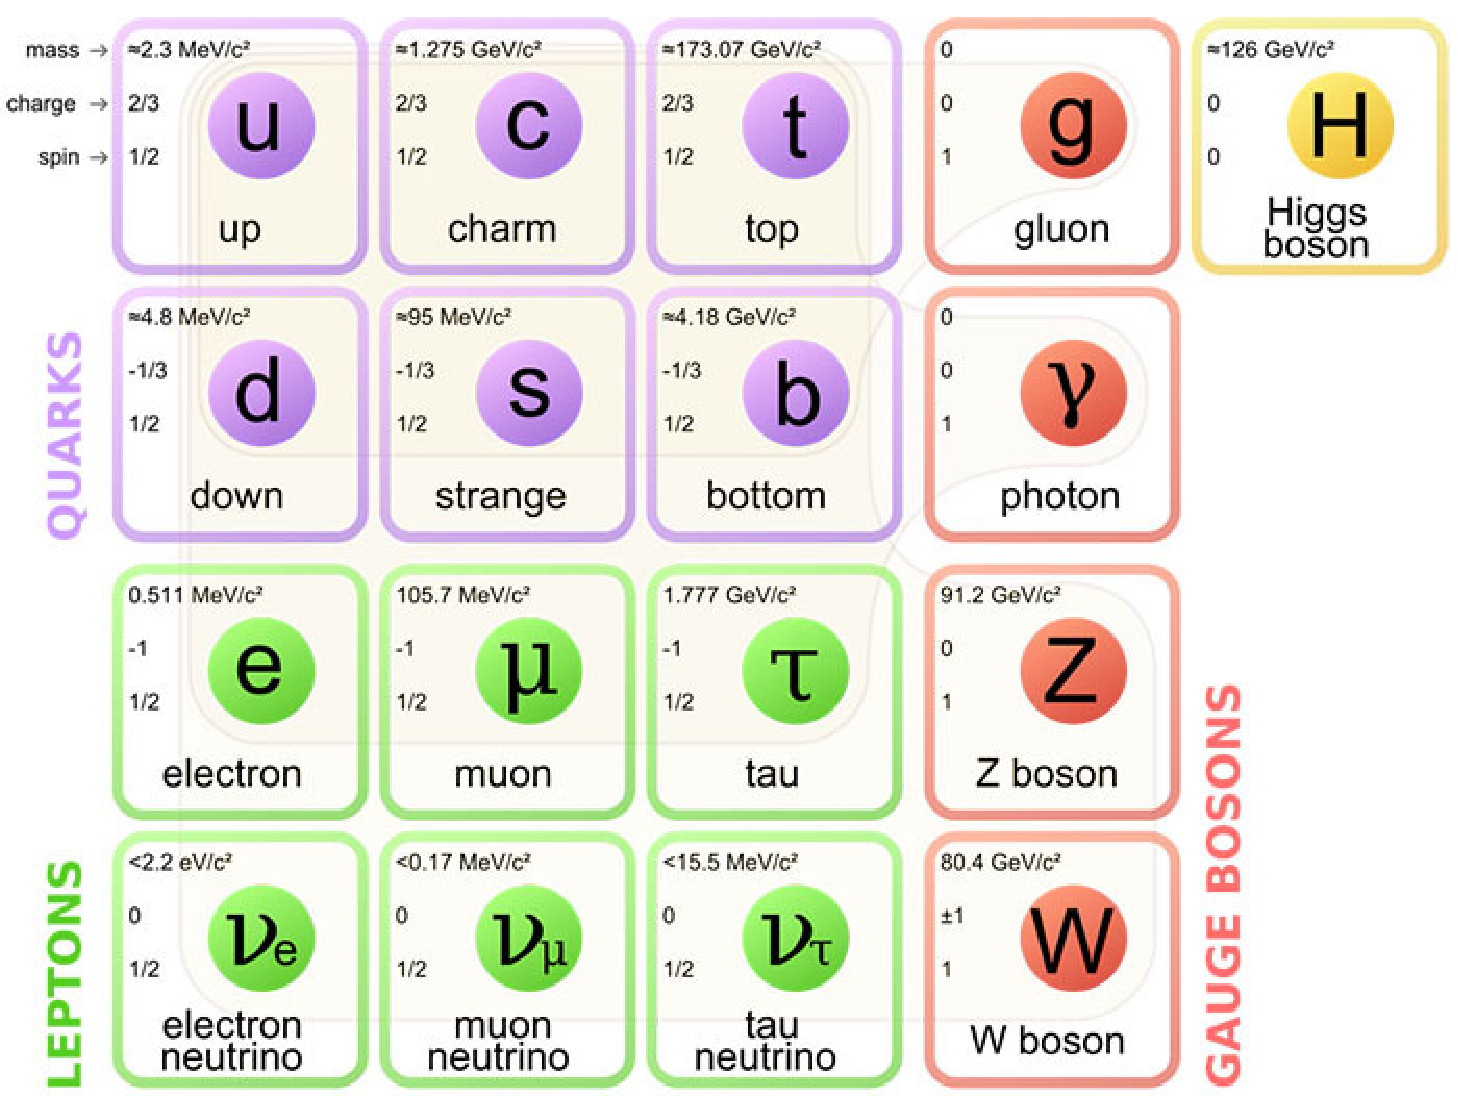
\includegraphics[width=0.75\textwidth]{StandardModel.pdf}
 	\caption[Standard Model particles]{The fundamental particles of the Standard Model. There are three generations of quarks and leptons. Along with the five bosons, where four of them relate to the interactions of the three forces included in the SM: Electromagnetism, the Weak force, and the Strong force and the final being the Higgs boson.}
 	\label{SMParticles} 
\end{figure}
 
 \subsection{Quantum Field Theory}
 \label{QFT}
 
 The interactions of all these particle fields are described by quantized fields whose operators describe the creation and annihilation of particles. Each of the particle fields of the SM have a corresponding gauge boson which is described by a quantized gauge field, see Fig. \ref{SMParticles}. The most well-known particle field is the EM field and its interactions. In order to write a concise theory of the particles in the SM, the symmetry and conservation laws of the SM can be derived by starting with Noether's Theorem.
 
 \subsection{Noether's Theorem}
 
 Noether's theorem states,"to each symmetry of a local Lagrangian, there corresponds a conserved current" \cite{peskin_introduction_1995}. This can be done by allowing for an infinitesimal symmetry variation. Requiring the Lagrangian to be invariant under $\phi(x)\rightarrow\phi^\prime(x)=\phi(x)+\alpha\Delta\phi(x)$, where $\alpha$ is infinitesimal real parameter and $\Delta\phi$ is a deformation to the field, up to a 4-divergence, the Lagrangian transforms as,
 \begin{equation}\label{LagrangeFluctuation}
 \mathcal{L}(x)\rightarrow\mathcal{L}(x)+\alpha\partial_\mu\mathcal{J}^\mu(x),
 \end{equation}
 where $\mathcal{J}^\mu$ is a current. If we apply the Euler-Lagrange equation,
 \begin{equation}
 \partial_\mu(\frac{\partial\mathcal{L}}{\partial(\partial_\mu\phi)})-\frac{\partial\mathcal{L}}{\partial\phi}=0,
 \end{equation}
 to Eqn. \ref{LagrangeFluctuation} with the addition of the fluctuation of the particle field. After some simplification we get a conserved current \cite{halzen_quarks_1984, peskin_introduction_1995},
 \begin{equation}
 \begin{split}
 \partial_\mu j^\mu(x)&=0, \text{ where}\\
 j^\mu(x)&=\frac{\partial\mathcal{L}}{\partial(\partial_\mu\phi)}\Delta\phi-\mathcal{J}^\mu
 \end{split}.
 \end{equation} We see from the above equation that the current $j^\mu(x)$ of the Lagrangian is conserved. Now let's apply this to the particle fields of the SM.
 
 \subsection{Quantum Electrodynamics (QED)}
 
 First, we start with the assumption that the wave function $\psi(x)$ should transform as,
 \begin{equation}\label{U1gauge}
 \psi(x)\rightarrow e^{i\alpha(x)}\psi(x),
 \end{equation}
 where $\alpha(x)$ has an arbitrary dependence on space and time. 
 If one were to include this into the Lagrangian for a spin-$1/2$ particle in a vacuum,
 \begin{equation}\label{DiracLag}
\mathcal{L}_{QED}^{vac}=i\overline{\psi}\gamma^\mu\partial_\mu\psi-m\overline{\psi}\psi
\end{equation}
 where the $\gamma^\mu$ are the Dirac matrices, $\partial_\mu$ is the partial derivative, $\overline{\psi}$ is the hermitian conjugate of the wave function $\psi$, and $m$ is the mass of the particle. As a small aside, the bilinear quantities $\overline{\psi}(4\times4)\psi$ have certain properties under Lorentz transformations when the $4\times4$ matrix is a $\gamma$-matrices. These are of the form,
\begin{equation} \label{gammaMatrix}
\gamma^0=
\begin{bmatrix}
\boldsymbol{I} & 0 \\
0 & -\boldsymbol{I}
\end{bmatrix},
\boldsymbol{\gamma}=
\begin{bmatrix}
0 & \boldsymbol{\sigma} \\
-\boldsymbol{\sigma} & 0
\end{bmatrix},
\gamma^5=
\begin{bmatrix}
0 & \boldsymbol{I} \\
\boldsymbol{I} & 0
\end{bmatrix},
\end{equation}
where the $\boldsymbol{I}$ is the identity matrix and $\boldsymbol{\sigma}$ are the Dirac matrices. We can combine the first two parts of Eqn. \ref{gammaMatrix} and write it compactly as $\gamma^\mu$ where $\mu=0,1,2, \text{and }3$. The possible interesting quantities of the above transformations are shown in Table \ref{Transformations}.

\begin{table}
\centering
\begin{tabular}{|c|c|c|c|}
\hline
Type & Form & Components & Space Inversion \\
\hline
\hline
 Scalar &  $\overline{\psi}\psi$ &  1 & $+$ under $P$ \\
 Vector & $\overline{\psi}\gamma^\mu\psi$ & 4 & Space compts.: $-$ under $P$ \\
 Tensor & $\overline{\psi}\sigma^{\mu\nu}\psi$ & 6 &  \\
 Axial Vector & $\overline{\psi}\gamma^5\gamma^\mu\psi$ & 4 & Space compts.: $+$ under $P$ \\
 Pseudoscalar & $\overline{\psi}\gamma^5\psi$ & 1 & $-$ under $P$ \\
 \hline
\end{tabular}
\caption[Fermion Currents]{A table showing all forms of the fermion currents. These can be symmetric under parity transformation in all or some components.}
\label{Transformations}
\end{table}

To allow for the field to be invariant, we must include a derivative, $D_\mu$, that is covariant under phase transformations,
 \begin{equation}\label{QEDCovariantD}
 D_\mu\equiv\partial_\mu-ieA_\mu.
 \end{equation}
 The covariant derivative includes the vector field $A_\mu$ which must also transform as,
  \begin{equation}\label{PhotonField}
 A_\mu\rightarrow A_\mu+\frac{1}{e}\partial_\mu\alpha.
 \end{equation}
 So after requiring that there be a local gauge transformation, we were forced to introduce a vector field $A_\mu$, called the gauge field, which couples to Dirac particles in the same way as the photon field. We will think of this new field as the real photon field, which means we need to add a kinematic energy portion to the Lagrangian. This kinematic term will be invariant under Eqn. \ref{PhotonField}, which leads us to the final representation of the QED Lagrangian which can be written down concisely as, 
\begin{equation}\label{LagrangianQED}
\mathcal{L}_{QED}=\overline{\psi}(i\gamma^\mu\partial_\mu-m)\psi+e\overline{\psi}\gamma^{\mu}A_{\mu}\psi-\frac{1}{4}F^{\mu\nu}F_{\mu\nu},
\end{equation}
where $A_{\mu}$ is the EM field operator and $F^{\mu\nu}$ is the EM field tensor. This Lagrangian describes the interactions between spin-$1/2$ charged particles and the $U(1)$ EM force. Each of the parts of this equation is Lorentz invariant which allows this to be true in all reference frames. 

\begin{figure}
 	\centering
	\includegraphics[width=0.75\textwidth]{QEDRules.png}
 	\caption[QED Feynman Diagrams]{The possible Feynman diagrams in QED. The $e$ can be replaced with any spin-$1/2$ charged particle. We see that the electron and photon can propagate freely in space or a vertex with one photon and a particle-antiparticle pair is allowed.}
 	\label{QEDRules} 
\end{figure}

From the QED Lagrangian Eqn. \ref{LagrangianQED}, we see that particles that interact electromagnetically can interact with the photon. This can be shown as a Feynman diagram, see Fig. \ref{QEDRules}, which has a vertex interaction with a photon and a particle-antiparticle pair. These, and the inclusion of freely moving particles, are the basic types of Feynman diagrams for QED. 

\subsection{Quantum Chromodynamics}

Let's now transition from the description of the $U(1)$ EM field to the $SU(3)$ Quantum Chromodynamic (QCD) field and the transformation of quark fields. A quark in a vacuum is described by,
\begin{equation}\label{LagrangianQCDVacuum}
\mathcal{L}_{QCD}^{vac}=\overline{q}_j(i\gamma^\mu\partial\mu-m)q_j,
\end{equation}
where $q_1, q_2,$ and $q_3$ are quark fields with three possible color charges. From this we want to require that the field is again invariant under another local phase transformation such as,
\begin{equation}
q(x)\rightarrow Uq(x)\equiv e^{i\alpha_a(x)T_a}q(x),
\end{equation}
where $U$ is a $3\times3$ unitary matrix, $T_a$ with $a=1,\ldots,8$ are a set of linearly independent traceless $3\times3$ matrices, and $\alpha_a$ are the group parameters. Since the generators $T_a$ do not necessarily commute with each other, we can see that it is a non-Abelian transformation and the commutator can be represented as,
\begin{equation}
[T_a, T_b]=if_{abc}T_c,
\end{equation}
where $f_{abc}$ are constants. 

We need to impose $SU(3)$ local gauge invariance on Eqn. \ref{LagrangianQCDVacuum}, to allow for the following phase transformations,
\begin{equation}
\begin{split}
& q(x)\rightarrow(1+i\alpha_a(x)T_a)q(x), \\
& \partial_\mu q\rightarrow(1+i\alpha_aT_a)\partial_\mu q+iT_aq\partial_\mu\alpha_a.
\end{split}
\end{equation}
From this is seems straight forward that we can proceed in exactly the same manner as QED, which is to add a transformation to the derivative,
\begin{equation}
D_\mu=\partial_\mu+ig_Q T_aG_\mu^a,
\end{equation}
where the field $G_\mu^a$, which are the gluons, transforms as, 
\begin{equation}
G_\mu^a\rightarrow G_\mu^a-\frac{1}{g_Q}\partial_\mu\alpha_a,
\end{equation}
where $g_Q$ is the coupling strength of QCD interactions. This will give us a similar Lagrangian to the QED one described above, but this is not sufficient for a non-Abelian gauge transformation and it does not produce a gauge-invariant Lagrangian. One final transformation is required for the $G_\mu^a$ fields, 
\begin{equation}\label{QCDGaugeTransform}
G_\mu^a\rightarrow G_\mu^a-\frac{1}{g_Q}\partial_\mu\alpha_a-f_{abc}\alpha_b G_\mu^c.
\end{equation}

\begin{figure}[!htb]
	\minipage{0.4\textwidth}
	  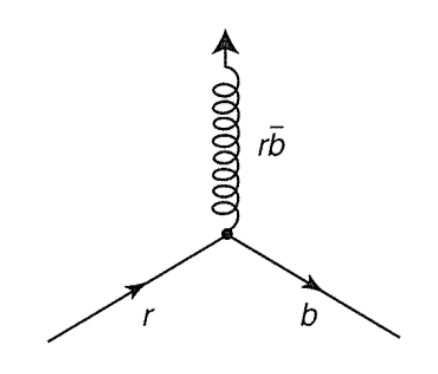
\includegraphics[width=\linewidth]{QCDQuarkRules.png}
	\endminipage\hfill
	\minipage{0.5\textwidth}
	  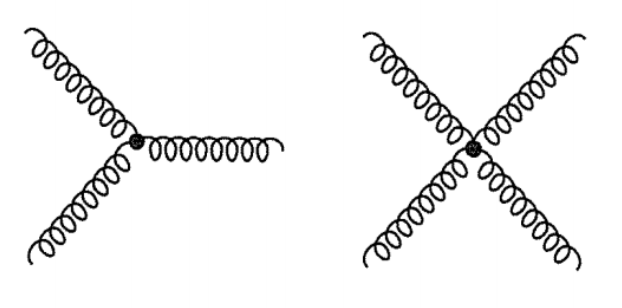
\includegraphics[width=\linewidth]{QCDGluonRules.png}
	\endminipage\hfill
	\caption[QCD Feynman Diagrams]{The possible Feynman diagrams in QCD where each vertex needs to conserve color charge. Here is just an example of a red-blue vertex. QCD also includes a 3- and 4-vertex with gluons.}
 	\label{QCDRules} 
\end{figure}

This finally gives us a gauge invariant kinetic energy term for all the $G_\mu^a$ fields and thus we can write the QCD interactions as,
\begin{equation}\label{LagrangianQCD}
\mathcal{L}_{QCD}=\overline{q}(i\gamma^\mu\partial_\mu-m)q-g_Q(\overline{q}\gamma^\mu T_a q)G^a_\mu-\frac{1}{4}G^a_{\mu\nu}G_a^{\mu\nu}.
\end{equation}
From the QCD Lagrangian Eqn. \ref{LagrangianQCD}, we can see that it includes all of the same interactions we showed for QED, but also includes a $SU(3)$ interaction due to the quark-gluon interactions with a certain color charge, see Fig. \ref{QCDRules}. However, QCD also included a 3- and 4-vertex interaction between the gluons, which arises due to the non-Abelian nature of the force. From this, it is easy to tell that QCD is a much more complicated theory. We seem to be missing a vital part of the SM, specifically a theory for the Weakly interacting processes which is mediated by the massive bosons, \W{} and \Z{} from Fig. \ref{SMParticles}. 

\subsection{Weak Force}
\label{WeakForce}

The Weak force is responsible for nuclear decay. The Weak force has an interaction of the type $\frac{1}{2}\gamma^\mu(1-\gamma^5)$, so it is a $V-A$ interaction with $SU(2)$ symmetry. From this, we can conclude that it violates Parity (P). Parity is a transformation from $(x, y, z)\rightarrow(-x,-y,-z)$ or space inversion. Since it violates Parity, the next step is to consider a conservation of $CP$, where $C$ is charge conjugation (particle-to-antiparticle). 

Now the Weak force is mediated by two vector bosons, \W{} and \Z, see Fig. \ref{SMParticles}. These are unlike the other forces because these vector bosons have a large mass of $m_\W=80.379\pm0.012$ GeV and $m_Z=91.1876\pm0.0021$ GeV. The \W{} boson is a charged particle and interacts with many nuclear decays. 

\begin{figure}
 	\centering
	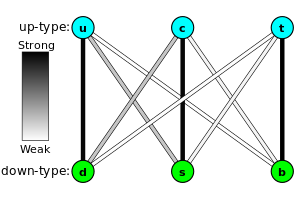
\includegraphics[width=0.5\textwidth]{Quark_weak_interactions.png}
 	\caption[CKM Matrix Couplings]{A grammatical representation to show the couplings for Weak interactions, known as the Cabibbo-Kobayashi-Maskawa Matrix. }
 	\label{CKMInteractions} 
\end{figure}

The \W{} boson interacts very interestingly for quarks in the SM. There is a mixing of flavors of quarks for particles. They will mix partners between up-type and down-type particles, see Fig. \ref{CKMInteractions} \cite{kobayashi_cp-violation_1973}. The interactions for the generalized three generations of quarks is known as the Cabibbo-Kobayashi-Maskawa (CKM) matrix,
\begin{equation}\label{CKM}
\begin{bmatrix}
d' \\
s' \\
b' \\
\end{bmatrix} =
\begin{bmatrix}
V_{ud} & V_{us} & V_{ub} \\
V_{cd} & V_{cs} & V_{cb} \\
V_{td} & V_{ts} & V_{tb} \\
\end{bmatrix}
\begin{bmatrix}
d \\
s \\
b \\
\end{bmatrix},
\end{equation}
where for example, $V_{ud}$ is the coupling of $u$ to $d$ which is exactly $(d\rightarrow u+W^-)$. This matrix can be reduced to a form which has three generalized Cabibbo angles $(\theta_{12},\theta_{23},\theta_{13})$ and a phase factor $(\delta)$. The coupling between the third generation does not mix with the other two generations. For the moment, we can only determine these values from experimentation. 

\begin{figure}[!htb]
	\minipage{0.4\textwidth}
	  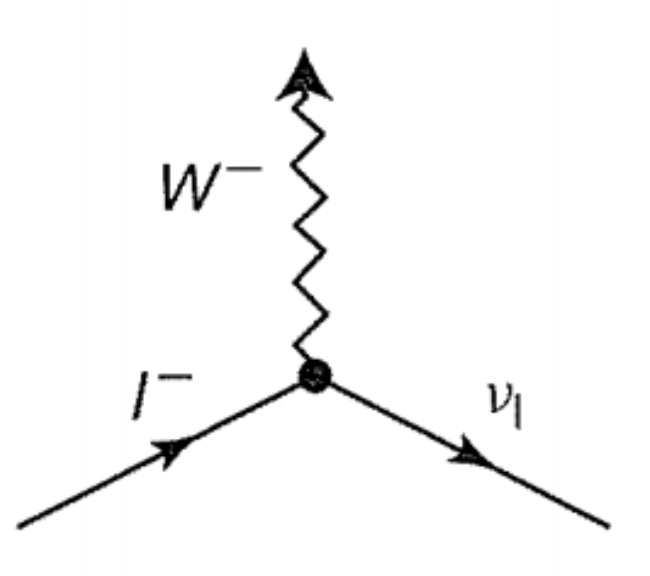
\includegraphics[width=\linewidth]{Wboson_interactions.png}
	\endminipage\hfill
	\minipage{0.4\textwidth}
	  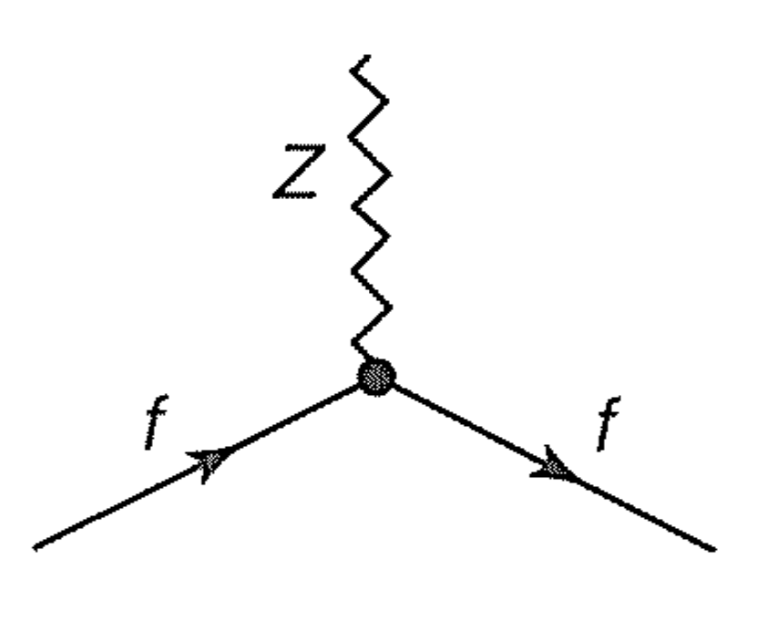
\includegraphics[width=\linewidth]{Zboson_interaction.png}
	\endminipage\hfill
	\caption[Weak Feynman Diagrams]{Feynman diagram for Neutral Weak interaction and the charged Weak current.}
 	\label{WeakRules} 
\end{figure}

The \Z{} boson is known as the neutral current. This boson mediates forces between particles and their respective antiparticles, see Fig. \ref{ZbosonInteraction}. This interaction for the neutral weak force is $\gamma^\mu(c_V^f-c_A^f\gamma^5)$ which is quite similar to the charged weak interaction, but differs by the constants $c_V^f$ and $c_A^f$. The Weak interactions are shown in Fig. \ref{WeakRules}. We see the charged \W{} boson interacts with the charged leptons and their respective neutrinos or allows for flavor changing interactions with quarks. Even though the neutral \Z{} boson interacts with a $V-A$ interaction we can still replace the $\gamma$ in any QED Feynman diagram with a \Z{}.

\subsection{The Electroweak Lagrangian}

The simplest group for the Electroweak interaction is $SU(2)_L\times U(1)_Y$, which will give the left-handed interactions in doublets with the addition of massive gauge bosons \W{} and \Z{} with a massless photon. We first consider the free Lagrangian,
\begin{equation}\label{WeakL}
\mathcal{L}=\overline{\psi}_j\gamma^\mu\psi_j,
\end{equation}
where $j$ is the fermion wave function. We are not including the mass parameter because it would cause the left and right-handed parts to mix.  This is assumed to transform under the global invariant,
\begin{equation}\label{WeakGlobal}
\begin{split}
\chi_L\rightarrow\chi'_L&=e^{i\frac{\tau_a}{2}\alpha^a(x)+i\beta(x)Y}\chi_L, \\
\psi_R\rightarrow\psi'_R&=e^{i\beta(x)Y}\psi_R
\end{split}
\end{equation}
where the transformation $e^{i\frac{\tau_a}{2}\alpha^a(x)}$ with $a = 1, 2, 3$ is the $SU(2)_L$ transformation and only acts on the left-handed doublet. The next step is to require that the Lagrangian is invariant under local $SU(2)_L\times U(1)_Y$. We allow for the following covariant derivatives,
\begin{equation}
\begin{split}
D_\mu\psi_1&=[\partial_\mu-ig_W\frac{\tau_a}{2}W_\mu^a-ig_W^\prime y_1 B_\mu]\psi_1 \\
D_\mu\psi_2&=[\partial_\mu-ig_W^\prime y_2 B_\mu]\psi_2 \\
D_\mu\psi_3&=[\partial_\mu-ig_W^\prime y_3 B_\mu]\psi_3 \\
\end{split},
\end{equation}
where $g_W$ and $g_W^{\prime}$ are the Weak force coupling constants while $W_\mu^a$ and $B_\mu$ are four gauge bosons and can be the possible candidates for $\W^\pm$, $Z$ and $\gamma$. 

 Just like the above descriptions, the fields need to transform along with the wave functions and derivatives. These transformations are,
\begin{equation}
\begin{split}
B_\mu\rightarrow&B^\prime_\mu=B_\mu+\frac{1}{g_W^\prime}\partial_\mu\beta(x) \\
W\mu\rightarrow&W^\prime_\mu=U_L W_\mu U^\dagger_L-\frac{1}{g_W}\partial_\mu U_L U_L^\dagger \\
\end{split},
\end{equation}
where $U_L=e^{i\frac{\tau_a}{2}\alpha^a(x)}$. These transformations are similar to the QED and QCD transformation. If we include all of these invariant transformations in the free Weak Lagrangian Eqn. \ref{WeakL}, we get a free invariant Lagrangian, but this does not allow us to include a mass term for the fermions. Therefore, it is not a viable procedure to include the Electroweak interactions into the model. In order to do this we must include the Higgs Mechanism.

\subsection{The Higgs Mechanism}\label{HiggsMechanism}

We are interested in the spontaneous symmetry breaking of a local $SU(2)$ group. Specifically, the following Lagrangian,
\begin{equation}\label{HiggsLagrangian}
\mathcal{L}=(\partial_\mu\phi)^\dagger(\partial^\mu\phi)-\mu^2\phi^\dagger\phi-\lambda(\phi^\dagger\phi)^2,
\end{equation}
with $\phi$ being a $SU(2)$ doublet of complex scalar fields,
\begin{equation}
\phi=\frac{1}{2}
\begin{bmatrix}
\phi_1+i\phi_2 \\
\phi_3+i\phi_4
\end{bmatrix},
\end{equation} 
and is invariant under global $SU(2)$ phase transformations $\phi\rightarrow e^{i\alpha_a\tau_a/2}\phi$. To allow for local invariance, we first allow for a covariant derivative,
\begin{equation}
D_\mu=\partial_\mu+ig_W \frac{\tau_a}{2}W_\mu^a,
\end{equation}
where we now have three gauge fields, $W_\mu^a$. If we assume an infinitesimal gauge transformation for the $SU(2)$ doublet $\phi(x)\rightarrow\phi'(x)=(1 +i\frac{\tau_a}{2}\alpha^a(x))\phi(x)$, then the gauge fields will transform as,
\begin{equation}\label{HiggVectorTransform}
W^a_\mu\rightarrow W^a_\mu-\frac{1}{g_W}\partial_\mu\alpha_a-f_{abc}\alpha_bW^c_\mu.
\end{equation}

You can see that Eqn. \ref{HiggVectorTransform} is similar to Eqn. \ref{QCDGaugeTransform} where we have replaced the QCD gauge field with the three gauge fields $W_\mu^a$. If we include these locally invariant transformations into the above $SU(2)$ Lagrangian we get,
\begin{equation}\label{WeakLagrangian}
\mathcal{L}=(\partial_\mu\phi+ig_W\frac{1}{2}\tau_{a}W^{a}_\mu\phi)^\dagger(\partial^\mu\phi+ig_W\frac{1}{2}\tau_{a}W^{a\mu}\phi)-\mu^2\phi^\dagger\phi+\lambda(\phi^\dagger\phi)^2-\frac{1}{4}W^{a}_{\mu\nu}W^{a\mu\nu},
\end{equation}
where the gauge field kinetic term has been included at the end. The most interesting regions of this Lagrangian is when $\mu^2<0$ and $\lambda>0$, and the potential has a minimum at $\phi^\dagger\phi=-\frac{\mu^2}{2\lambda}$. With this, we will expand the potential around the minimum and require that,
\begin{equation}
\phi_1=\phi_2=\phi_4=0, \phi_3^2=-\frac{\mu^2}{2\lambda}\equiv v^2.
\end{equation}
This is the spontaneous symmetry breaking of the $SU(2)$ symmetry, because of this we are able to substitute an expansion for the field,
\begin{equation}
\phi=\sqrt{\frac{1}{2}}
\begin{bmatrix}
0 \\
v+h(x)
\end{bmatrix},
\end{equation}
with this specific transformation of the $SU(2)$ doublet and the simplification of Eqn. \ref{WeakLagrangian}, the only remaining field is $h(x)$ which is referred to as the Higgs field. This is what is known as the Higgs Mechanism for a $SU(2)$ symmetry. 

\subsection{Electroweak} \label{EMWeak}

We want to include the Higgs Mechanism into the weak isospin and weak hypercharge, $SU(2)_L\times U(1)_Y$, transformations of electroweak interactions. Weak isospin and hypercharge is defined as $I_3=\frac{1}{2}(n_u-n_d)$ and $Y\equiv B+S$, respectfully, where $n_u,n_d$ is the number of up or down quarks, $B$ is the baryon number, and $S$ is the strangeness. The weak isospin triplet for weak currents can be written down using Eqn. \ref{WeakLagrangian}, 
\begin{equation}\label{WeakIsospinCurrent}
J_\mu^i(x)=\overline{\chi}_L\gamma_\mu\frac{1}{2}\tau_i\chi_L, \text{ with } i=1,2,3.
\end{equation}
Since this is a current we can calculate the charge by integrating all of space, $T^i=\int J_0^i(x)d^3x$, which will give us the generators of the $SU(2)_L$ symmetry $[T^i,T^j]=i\epsilon_{ijk}T^k$. Weak hypercharge, $Y$, is then defined by $Q=T^3+\frac{Y}{2}$ where $Q$ is the charge and $T^3$ is the third component of the weak isospin. The weak hypercharge is the conserved quantity of the $U(1)_Y$ symmetry. 

First, we need to include the coupling of the Weak current $J^a_\mu$ and the gauge field $W^{a\mu}$ such that,
\begin{equation}
-ig_WJ^a_\mu W^{a\mu}=-ig_W\overline{\chi}_L\gamma_\mu T^aW^{a\mu}\chi_L,
\end{equation}
which is the basic interaction for the $SU(2)_L$ symmetry. In this basic interaction, we can see that the electric charge that we know from EM is a combination of the Weak isospin and hypercharge and the gauge bosons mix to produce the massless photon that couples to the electric charge. There are three additional massive bosons, one neutral and two charged, that couple to the other combinations of Weak isospin and hypercharge. Then, we also need to include the weak hypercharge current with the fourth vector boson $B^\mu$,
\begin{equation}
-i\frac{g_W^{\prime}}{2}j_\mu^YB^\mu=-ig_W^{\prime}\overline{\psi}\gamma_\mu\frac{Y}{2}\psi B^\mu, 
\end{equation}
where the operators $T^a$ and $Y$ are generators for the $SU(2)_L$ and $U(1)_Y$ gauge transformations, respectively. Now we combine the two symmetries with the transformations of the left and right hand components of $\psi$ and from this we can write down the contributions of the two gauge fields $W_\mu^3$ and $B_\mu$ and the missing angle $\theta_W$ to find the interactions of the two neutral currents. The physical fields are thus,
\begin{equation}
-ig_WJ_\mu^3W^{3\mu}-i\frac{g_W^{\prime}}{2}j_\mu^YB^\mu=-iej_\mu^{em}A^\mu-\frac{ie}{sin\theta_Wcos\theta_W}[J_\mu^3-sin^2\theta_Wj_\mu^{em}]Z^\mu.
\end{equation}

From this we can write down the Electroweak Lagrangian, for any fermion that interacts with the field. Moreover, we can formulate the Higgs mechanism, such that we can calculate the theoretical masses of the gauge bosons and fermions as, 
\begin{equation}
\begin{split}
& M_\W=\frac{1}{2}vg_W \\
& M_\Z=\frac{1}{2}v\sqrt{g_W^2+g_W^{\prime 2}}.
\end{split}
\end{equation}
However, these masses cannot be predicted since they depend on the values from the chosen Higgs field. 

\subsection{The Standard Model Lagrangian}

With the inclusion of the Higgs mechanism and the formulation of a local gauge invariant Lagrangian for the Electroweak and QCD fields, we have the complete SM Lagrangian as,
\begin{equation}\label{SMLagrangian}
\begin{split}
\mathcal{L}=&-\frac{1}{4}W^a_{\mu\nu}W^{a\mu\nu}-\frac{1}{4}B_{\mu\nu}B^{\mu\nu}-\frac{1}{4}G^a_{\mu\nu}G_a^{\mu\nu} \\
&+\overline{L}\gamma^\mu(i\partial_\mu-g_{W}\frac{1}{2}\tau^{a}W^{a}_{\mu}-g^{\prime}_{W}\frac{Y}{2}B_\mu-g_{Q}T_{b}G^{b}_{\mu})L \\
&+\overline{R}\gamma^\mu(i\partial_\mu-g^{\prime}_{W}\frac{Y}{2}B_\mu-g_{Q}T_{b}G^{b}_{\mu})R \\
&+\lvert(i\partial_\mu-g_{W}\frac{1}{2}\tau^{a}W^{a}_\mu-g^{\prime}_{W}\frac{Y}{2}B_\mu)\phi\lvert^2-V(\phi) \\
&-(G_1\overline{L}\phi R+G_2\overline{L}\phi_cR+\text{hermitian conjugate}),
\end{split}
\end{equation}
where the first terms are the kinetic energies and self-interactions of the $\W^\pm,\Z, g, \text{and } \gamma$ bosons. The second and third terms are the kinetic energies and interactions of the leptons and quarks with the $\W^\pm,\Z, g, \text{and } \gamma$ bosons where $L$ is a left-handed fermion doublet and $R$ is a right-handed fermion singlet. The fourth term is the $\W^\pm,\Z,\gamma$ and Higgs masses and couplings. The final term is the lepton and quark masses and couplings to the Higgs field.  

\section{Fundamental Problems in the Standard Model}
\label{sec:SMIssues}

The SM is able to accurately and precisely describe many facets of the universe, whether it comes to predicting the existence of a sixth quark or the confirmation of $g - 2$ for the muon to 9 orders of magnitude. Unfortunately, there are some evidence of matter or interactions that cannot be described, such as dark matter, the Hierarchy problem, and a possible GUT. Let's look into each of these further.

\subsection{Dark Matter}
The main motivation for Dark Matter is the difference between the visible matter and the measurable matter in the universe. This has most notably been seen in the radial velocities of stars in galaxies. In a galaxy which is solely made up of visible matter, or matter that interacts with light, the radial velocity of stars should decrease as $1/\sqrt{r}$ the further away it is from the galactic nuclei, although measurements show the velocity becoming constant as a function of radius.

A study of this was on the galaxy NGC 1560, where the measured galactic velocity curve provided a result that was 400 times large than the visible matter in the cluster \cite{broeils_mass_1992}.  To reproduce these features in models, the mass of the galaxy must be significantly more than what is seen. This implies some unseen dark matter, that still interacts with the gravitational field, but not with the EM field. The neutrino could be a potential dark matter candidate due to the fact that it interacts weakly with matter and is abundant in the universe. However, the mass, which is nonzero, can only explain a small fraction of the dark matter in the universe where we have limits derived by high-redshift galaxies \cite{bertone_dark_2005}.

\begin{figure}
 	\centering
	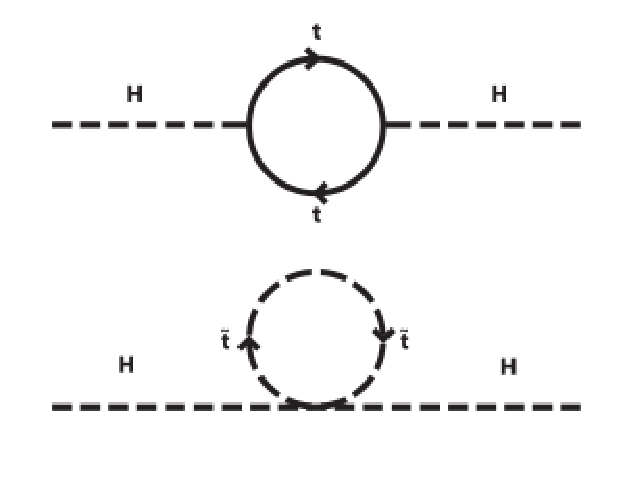
\includegraphics[width=0.5\textwidth]{Hierarchy.pdf}
 	\caption[Hierarchy Problem Loop Correction]{The loop corrections to the Higgs boson interacting with a top quark and its superpartner, the top squark. This is a next-to-leading order (NLO) correction to the Higgs boson mass.}
 	\label{HiggsMass} 
\end{figure}

\subsection{Hierarchy Problem} 
The Higgs boson is a beautiful solution to electroweak symmetry breaking, gives a method for particles to acquire mass, see Sec. \ref{HiggsMechanism},  and was discovered to have a measured mass of $m_{H}=125.18\pm0.16$ GeV \cite{chatrchyan_observation_2012}, \cite{aad_observation_2012}, \cite{chatrchyan_observation_2013}, \cite{atlas_collaboration_combined_2015}. This value, however, is not predictable with the SM, but can be constrained and leads to some inconsistencies when you include loop corrections. Since the Higgs boson is strongly coupled to particles with large masses, the dominant loop correction is due to interactions with the $t$ quark. These higher order loop corrections to the Higgs mass, $m_H^2$, caused by the fermionic $t$ loop, see Fig \ref{HiggsMass}, are,
\begin{equation} \label{HiggsDivergence}
\Delta m_{H}^{2}=-\frac{|\lambda_{t}|^{2}}{8\pi^{2}}\Lambda_{UV}^{2}+\cdot\cdot\cdot,
\end{equation}
where $\lambda_f$ is the vertex factor for the respective fermion and $\Lambda_{UV}$ is the ultraviolet momentum cutoff. The Higgs boson loop corrections are highly dependent on all virtual and real particles that couple to the Higgs field. We can see the corrections from Eqn. \ref{HiggsDivergence} from the $t$ quark will cause a large divergence. 

The quadratic divergence of the Higgs mass then requires a fine tuning of the parameters $\lambda_f$ to solve the divergence. This means the only way for the SM to reconcile this unfortunate fact is to have a relatively lucky cancellation of very large numbers of order $10^{32}$ with equally small numbers. Fortunately, if we add the contribution of a bosonic partner of the fermion the Higgs loop corrections reduce to \cite{martin_supersymmetry_1997},
\begin{equation}
\Delta m_{H}^{2}=\frac{\lambda_{S}}{16\pi^{2}}[\Lambda_{UV}^{2} - 2m_{S}^{2}ln(\Lambda_{UV}/m_{S})+\cdot\cdot\cdot].
\label{HiggsRenormalization}
\end{equation}
With the introduction of a scalar partner to the $t$, there is a logarithmic divergence to the Higgs boson mass and it can be renormalized through the normal methods.

\subsection{Grand Unified Theory}

The SM is able to accurately describe three of the fundamental sources at typical energy scales, 1 to $10^{4}$ GeV, but ideally the forces would be able to merge into a single force at higher energies. This has not been directly observed, but many theories, such as SUSY, can give a GUT that can allow for a common gauge coupling and a simpler theory overall \cite{martin_supersymmetry_1997}.

At standard energies for particle physics experiments the difference in the strength of each force is quite noticeable. But it has been shown that in the SM the strengths of each force are dependent on the energy scale. SUSY could also explain the running coupling constant for QCD interaction. It would be ideal if they converge to a single force at large energies, such as $10^{16}$ GeV. In Fig. \ref{GUT}, we see the extrapolated energy scales of the forces in the SM shown as the dotted line. These unfortunately, do not meet at a single point to become one force, but if we include SUSY into the model we get a nice convergence between the forces \cite{martin_supersymmetry_1997}.

\begin{figure}
 	\centering
	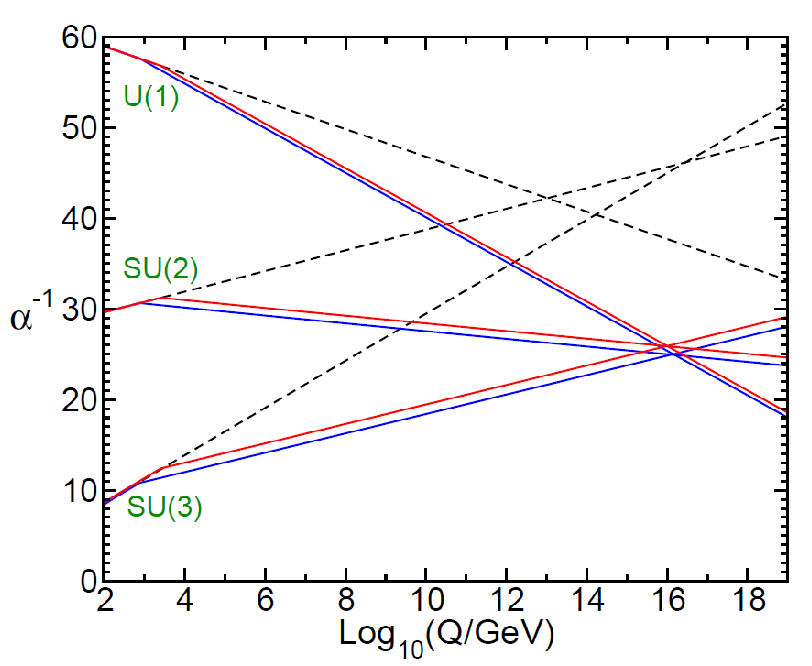
\includegraphics[width=0.5\textwidth]{GUTRenormalization.png}
 	\caption[GUT Force Energy Dependence]{The energy dependence of the inverse gauge coupling of each force in the SM (dashed line) and the MSSM (solid lines). The MSSM gives two thresholds for the sparticle mass 750 GeV and 2.5 TeV.}
 	\label{GUT} 
\end{figure}

\section{Supersymmetry}\label{sec:SUSY}

We have seen from the above three problems that there is still more to learn about the universe, such as dark matter and the hierarchy problem. SUSY \cite{ramond_dual_1971, volkov_possible_1972, wess_supergauge_1974, fayet_supergauge_1975, barbieri_gauge_1982, chamseddine_locally_1982, hall_supergravity_1983, kane_study_1994, noauthor_natural_nodate} also has the ability to be a potential GUT. We saw from the Hierarchy problem that the addition of a bosonic partner to a fermion will allow for the loop corrections to be renormalizable without fine tuning. Fortunately, some theories have allowed for such a problem to be solved. Namely, the theory of SUSY, which essentially states that each particle in the SM has a superpartner that has only the spin changed, that every fermion has a bosonic partner that has all the same quantum numbers except the spins differ by $1/2$, and vice-versa.

\begin{figure}
 	\centering
	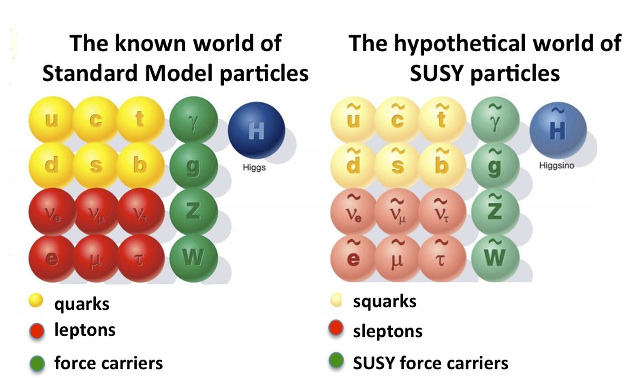
\includegraphics[width=0.75\textwidth]{SM-SUSY-diagram.jpg}
 	\caption[Supersymmetry and Standard Model Particles]{The corresponding SUSY particles which are partners to the SM particles.}
 	\label{SUSYParticles} 
\end{figure}

The partners to the fermions are denoted with a 's' in front of the name to notify that it is the scalar form of the particle and the partners to the bosons have an 'ino' attached at the end, such as photino, gluino, wino, and Higgsino. So, for the partners to the fermionic particles in the standard model we have: sup $(\widetilde{u})$, sdown $(\widetilde{d})$, scharm $(\widetilde{c})$, sstrange $(\widetilde{s})$, stop $(\st)$, and sbottom $(\widetilde{b})$ for the squarks and selectron $(\widetilde{e})$, smuon $(\widetilde{\mu})$, and stau $(\widetilde{\tau})$ for the charged sleptons. The partners to the neutrinos, which are always left-handed if you neglect the minimal masses, are sneutrinos $(\widetilde{\nu}_e, \widetilde{\nu}_\mu, \widetilde{\nu}_\tau)$, where we have one for each flavor of lepton, see Fig. \ref{SUSYParticles}. 

If the SUSY was unbroken, the superpartners would have exactly the same properties as the SM pairs except their spin. This would cause a massless photino or a $m_{\widetilde{e}}=0.511$ keV selectron. These particles would certainly have been detected at this point, which leads us to think that SUSY is a broken symmetry where all the superpartners have a mass that is significantly higher than their SM partners. 

\subsection{Supermultiplets and Chirality}
\label{subsec:chiral}

A supermultiplet is any symmetry where the number of bosonic degrees of freedom and fermionic degrees of freedom are equal, $n_B=n_F$. The simplest  way to achieve this is to have a combination of a single Weyl fermion, which is a chiral representation of the fermion and has two spin helicity states, $n_F=2$, and two real scalars with each having $n_B=1$. It becomes convenient for the mathematics to combine the two real scalars into one complex scalar field. Now the combination of a complex scalar field and a Weyl fermion is known as a chiral supermultiplet. 

\subsection{Minimal Supersymmetric Standard Model}
\label{sec:MSSM}

We have discussed how the fermions transform under the rules of SUSY, but how do the scalar field mediators translate into this new framework. First, we look at the Higgs boson. We know that there is not only one chiral supermultiplet. If there was only one in the electroweak gauge symmetry, with a Higgsino of spin-$1/2$, we would not have the anomaly cancellation of the traces, $Tr[T^2_3Y]\neq0$ and $Tr[Y^3]\neq0$, where $T_3$ is the third component of weak isospin and $Y$ is the weak hypercharge. In the SM, the traces of these for the fermions are already satisfied. So we must include two chiral supermultiplets of the Higgsino, with $Y=\pm\frac{1}{2}$, see Table \ref{ChiralSMultiplets}. 

It turns out that this is also necessary for the Higgsino field to give mass to different particles in the SM. A Higgs boson with $Y=1/2$ has the Yukawa couplings that allow it to interact with the up-type quarks $(u, c, t)$. Only a Higgs boson with $Y=-1/2$ has the correct Yukawa couplings to interact with the down-type quarks $(d, s, b)$ and the charged leptons $(e, \mu, \tau)$.

\begin{table}
 	\centering
	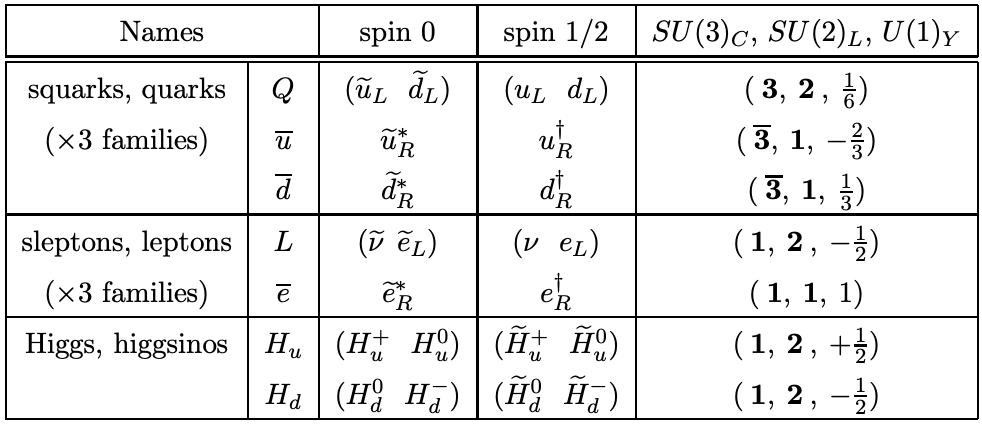
\includegraphics[width=0.7\textwidth]{ChiralSupermultiplets.png}
 	\caption[Chiral supermultiplets for fermions and bosons]{The chiral supermultiplets of the MSSM. Spin-0 fields are complex scalars and spin-$1/2$ fields are left-handed two component Weyl fermions \cite{martin_supersymmetry_1997}.}
 	\label{ChiralSMultiplets} 
\end{table}

\begin{table}
 	\centering
	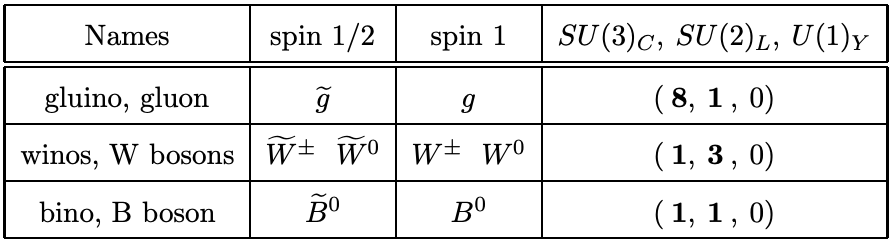
\includegraphics[width=0.7\textwidth]{GaugeSupermultiplets.png}
 	\caption[Chiral supermultiplets for gauge bosons]{The chiral supermultiplets of the MSSM \cite{martin_supersymmetry_1997}.}
 	\label{GaugeSMultiplets} 
\end{table}

The SM vector boson will also have a corresponding chiral supermultiplet. They have fermionic superpartners that are referred to as gauginos. The $SU(3)_C$ color gauge interactions of QCD, which are a spin-$1/2$ color-octet, has a partner called a gluino $(\widetilde{g})$. The electroweak gauge theory $SU(2)_L\times U(1)_Y$ has the superpartners $\widetilde{\W}^+,\widetilde{\W}^0, \widetilde{\W}^-, \text{and } \widetilde{B}^0$ each with spin-$1/2$, called winos and bino, see Table \ref{GaugeSMultiplets}. The gaugino mixtures of $\widetilde{\W}^0$ and $\widetilde{B}^0$ give the corresponding zino $(\widetilde{Z}^0)$ and photino $(\widetilde{\gamma})$. The chiral supermultiplets shown in Table \ref{ChiralSMultiplets} and \ref{GaugeSMultiplets} give the particles of the MSSM. 

The five higgsinos and electroweak gauginos mix with each other because of electroweak symmetry breaking \cite{martin_supersymmetry_1997}. The neutral higgsinos $(\widetilde{H}_u^0 \text{ and } \widetilde{H}_d^0)$ and neutral gauginos $(\widetilde{B} \text{ and } \widetilde{W}^0)$ mix into four mass eigenstates, which are called neutralinos, $\neutralino, \widetilde{\chi}^0_2, \widetilde{\chi}^0_3, \text{ and }\widetilde{\chi}^0_4$. The charged higgsinos $(\widetilde{H}_u^+ \text{ and } \widetilde{H}_d^-)$ and charged gauginos $(\widetilde{W}^+\text{ and } \widetilde{W}^-)$ can mix into two mass eigenstates with charge $\pm1$ called charginos,  $\widetilde{\chi}^\pm_1 \text{ and } \widetilde{\chi}^\pm_2$. 

\subsection{R Parity}
\label{subsec:rparity}

$R$-parity or matter parity is the multiplicatively conserved quantum number \cite{wess_supergauge_1974}, \cite{farrar_phenomenology_1978} defined as, 
\begin{equation} \label{RParity}
P_R=(-1)^{3(B-L)+2s}, 
\end{equation}
where $B$ is the baryon number, $L$ is the lepton number, and $s$ is the spin of the particle. From this we can find the $R$-parity of all the particles in the SM and MSSM. The definition of $R$-parity is quite useful because all the particles of the SM have an $R$-parity of $P_R=+1$, while all of the squarks, sleptons, gauginos, and higgsinos have $P_R=-1$.

$R$-parity is thought to be exactly conserved in SUSY, where there is no mixing between particles $(P_R=+1)$ and sparticles $(P_R=-1)$. This leads to three important consequences:
\begin{itemize}
	 \item The lightest sparticle that has $P_R=-1$ is called the "lightest supersymmetric particle" or LSP, which must be absolutely stable. It is a possible non-baryonic dark matter candidate.
	 \item Every sparticle, other than the LSP, must eventually decay into an odd number of LSPs.
	 \item For collider experiments, sparticles will only be produced in even numbers.
\end{itemize}
 We are going to be investigating a MSSM that conserves $R$-parity. This is quite well motivated by the possibility of a dark matter candidate \cite{feng_dark_2010}. 

\subsection{Mass Spectrums}\label{subsec:StopMassSpec}

\begin{figure}
\centering
	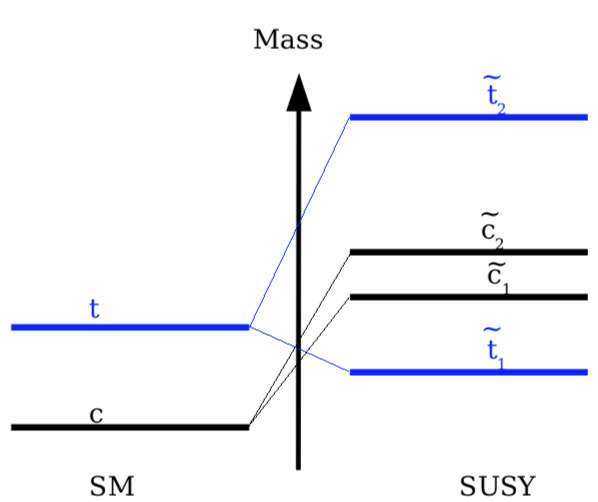
\includegraphics[width=0.5\textwidth]{TopSquarkMass.png}
 	\caption[Top squark mass hierarchy]{On the right we have the arbitrary masses of the top and charm quarks. The left and right handed states mix into two mass eigenstates. It is possible that the top squark will have the smallest mass of the squarks.}
 	\label{StopMass} 
\end{figure}

The third family of squarks and sleptons should have quite different masses compared to their first- and second-family counterparts, which is caused by the large Yukawa $(y_t, y_b, y_\tau)$ and soft $(a_t, a_b, a_\tau)$ couplings, which are holomorphic parameters proportional to the Yukawa couplings. This causes significant mixing between the chiral superpartners $(\widetilde{t}_L, \widetilde{t}_R), (\widetilde{b}_L. \widetilde{b}_R)\text{, and } (\widetilde{\tau}_L, \widetilde{\tau}_R)$. We will concentrate on how the mass of the top squark, \st{} evolves in the MSSM, given many contributions to the top squark mass such as, squared-mass terms, 4-vertex interactions terms with the up-type Higgs, the 3-vertex interactions with the down-type Higgs, and scalar potential couplings. We have a square-mass matrix for the top squarks, 
\begin{equation}
\mathcal{L}_{\text{stop masses}}=-
\begin{bmatrix}
\widetilde{t}_{1L}^* & \widetilde{t}_{1R}^* \\
\end{bmatrix}
\boldsymbol{m_{\st}^2}
\begin{bmatrix}
\widetilde{t}_{1L} \\
\widetilde{t}_{1R} \\
\end{bmatrix},
\end{equation}
where, 
\begin{equation}
\boldsymbol{m_{\st}^2}=
\begin{bmatrix}
m_{Q_3}^2+m_t^2+(\frac{1}{2}-\frac{2}{3}sin^2\theta_W)cos(2\beta)m_Z^2 & v(a_t^*sin\beta-\mu y_tcos\beta) \\
v(a_tsin\beta-\mu^*y_tcos\beta) & m^2_{\overline{u}_3} +m_t^2+(\frac{2}{3}sin^2\theta_W)cos(2\beta)m^2_Z \\ 
\end{bmatrix}.
\end{equation}

This is a hermitian matrix and can be diagonalized to give eigenstates $\st$ and $\widetilde{t}_2$ which are linear combinations of the left and right-handed \st, see Fig. \ref{StopMass}. Now we get the eigenvalues for the mass states as $m_{\st}^2<m_{\widetilde{t}_2}^2$. From this, models predict that the $\st$ is the lightest squark \cite{martin_supersymmetry_1997}. 

\subsection{SUSY Searches}
The SM of particle physics has been a powerful model for predicting interactions between quarks, leptons, and force carriers, with an accurate prediction for precision measurements, but has some faults such as, the Hierarchy problem, dark matter, and a Grand Unified Theory. We have seen that including SUSY can allow for possible solutions, such as; a dark matter candidate as the LSP, bosonic-fermionic loop corrections for the Higgs boson mass, and a unification of the fundamental forces at large energies. Then once investigating the theory of SUSY, we were able to determine that the top squark could be the lightest squark, which allows us to develop multiple searches for this proposed theory. 

\section{Current SUSY Results}\label{CurrentResults}

Here we see the most current results from searches for the top squark. These have been completed with data from 2016 with $35.9 \text{ fb}^{-1}$. This analysis was completed with the most up-to-date identification methods for particles in the SM. From this Analysis \cite{noauthor_search_nodate}, all 104 search region bins, as well as the corresponding single-lepton control region bins, the $\gamma+$jets control region bins and the QCD control regions, are fit simultaneously in order to evaluate the cross section excluded at 95\% confidence level for each signal benchmark point. 

The easiest way to think about the plots shown in Figs. \ref{T2ttANLimits}, \ref{T2bWANLimits}, \ref{T2tbANLimits}, \ref{T2fbdANLimits}, \ref{T2bWCANLimits} \cite{alwall_simplified_2009, alwall_model-independent_2009, feng_dark_2010}, is that there is a calculated limit for each mass point. The $x$-axis is the possible mass range for the \st, $m_{\st}$ and the y-axis is the possible range for the \neutralino, $m_{\neutralino}$. Each point in this 2D space has a color representation for the value of the upper limit on the cross section at a confidence level of 95\%. 

With the comprehensive analysis that was performed in 2016, we have various limits on the multiple decay modes of the \st{} which will be covered completely in Section \ref{ch:Search}. The comprehensive limits on the \st{} mass range from values of 550 to 1.1 \TeV{} for all of the all-hadronic decay modes. The CMS Collaboration has also combined the limits from the separate analyses which concentrate on the 1-lep, 2-lep, MT2, and HT missing analyses. The combination of these has shown that we can set limits on the \st{} mass range for masses of 800 to 1100 \GeV. 

\begin{figure}
\centering
	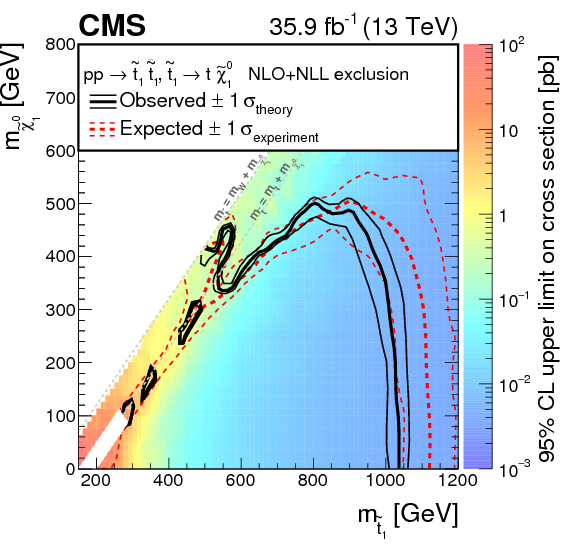
\includegraphics[width=0.50\textwidth]{T2tt_AN16.png}
 	\caption[T2tt Limits]{Limits for the mass parameter space for $\st\rightarrow t \neutralino$ (T2tt) decays. With a current limit of 1.05 \TeV{} for a minimal neutralino mass \cite{noauthor_search_nodate}.}
 	\label{T2ttANLimits} 
\end{figure}

\begin{figure}
\centering
	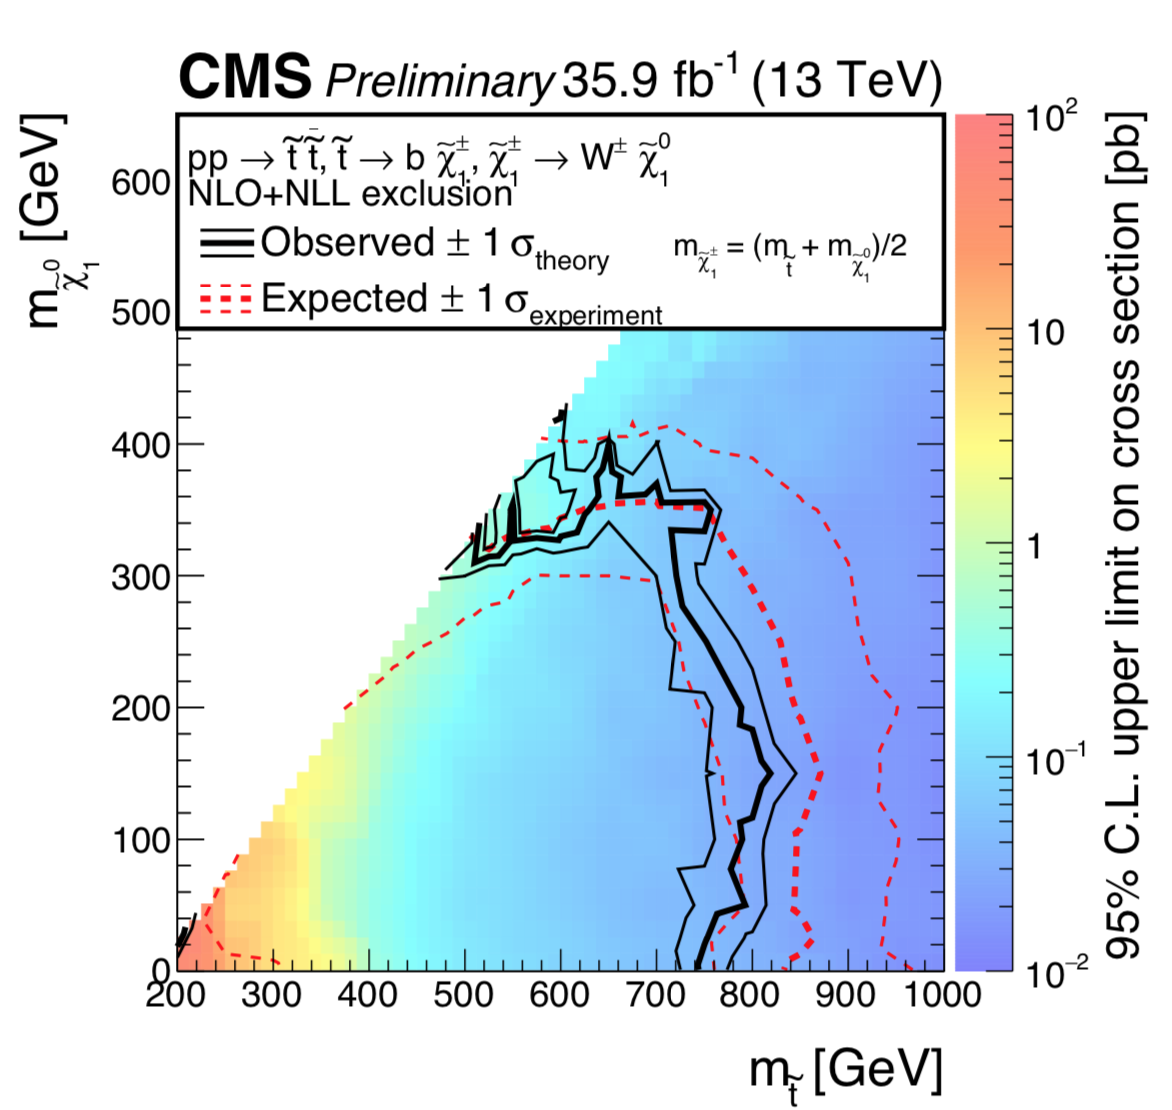
\includegraphics[width=0.50\textwidth]{T2bW_AN16.png}
 	\caption[T2bW Limits]{Limits for the mass parameter space for $\st\rightarrow b \chargino$ (T2bW) decays. With a current limit of 750 \GeV{} for a minimal neutralino mass \cite{noauthor_search_nodate}.}
 	\label{T2bWANLimits} 
\end{figure}

\begin{figure}
\centering
	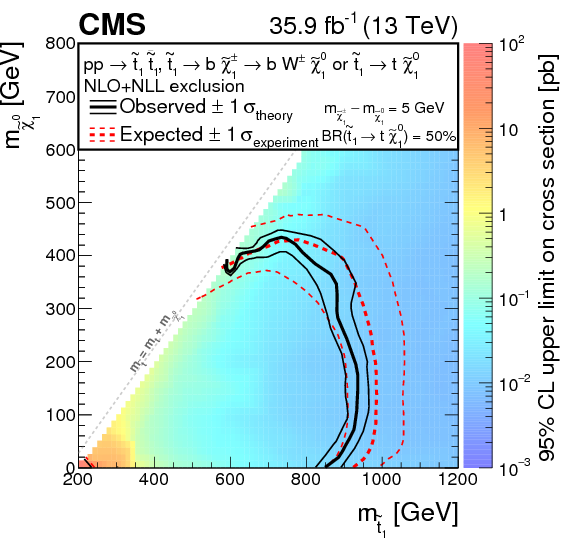
\includegraphics[width=0.50\textwidth]{T2tb_AN16.png}
 	\caption[T2tb Limits]{Limits for the mass parameter space for $\st\rightarrow b \chargino\rightarrow bW^\pm\neutralino$ or $\st\rightarrow t\neutralino$ (T2tb) decays. With a current limit of 850 \GeV{} for a minimal neutralino mass \cite{noauthor_search_nodate}.}
 	\label{T2tbANLimits} 
\end{figure}

\begin{figure}
\centering
	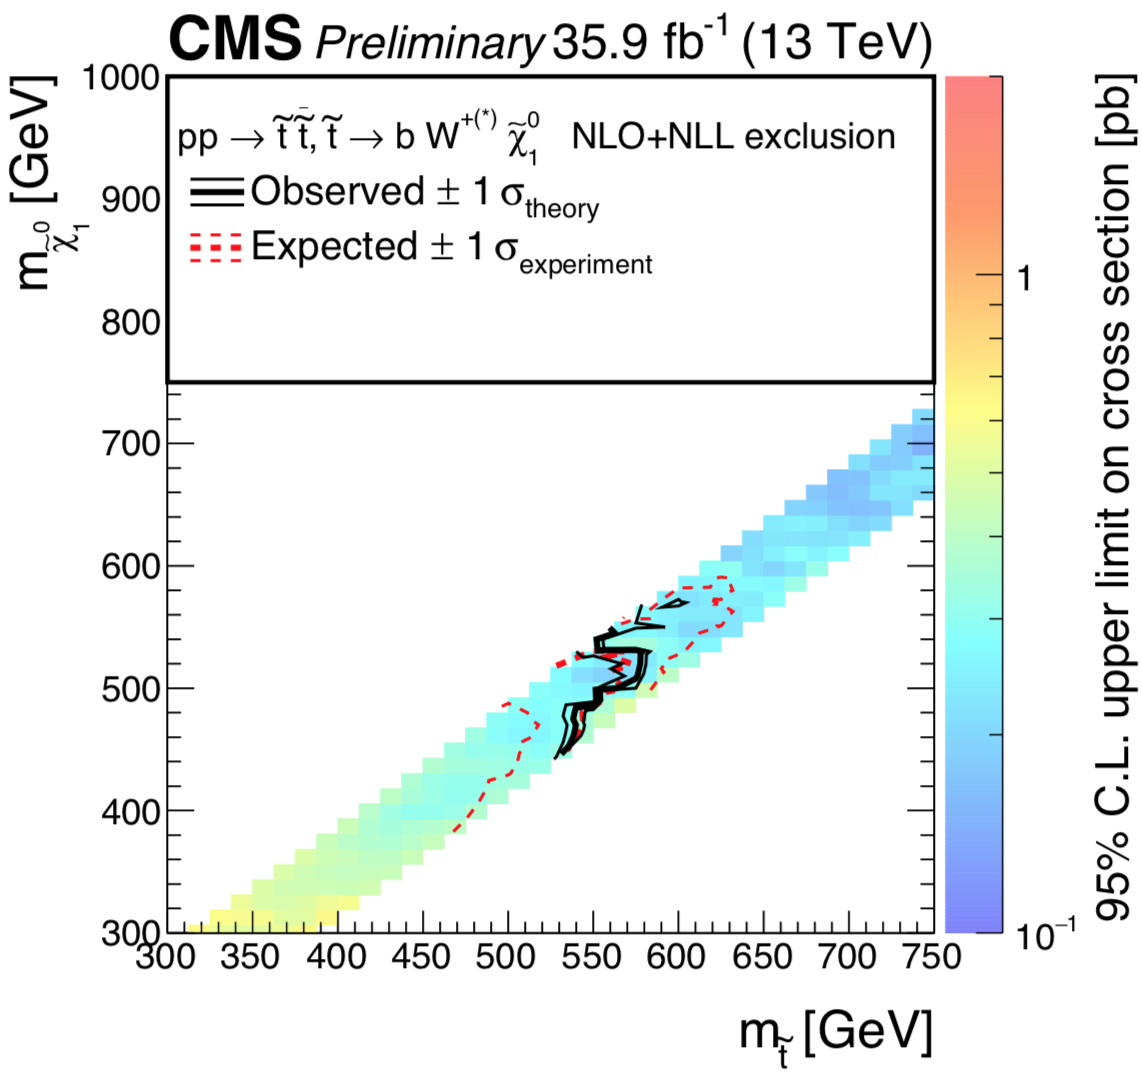
\includegraphics[width=0.50\textwidth]{T2fbd_AN16.png}
 	\caption[T2fbd Limits]{Limits for the mass parameter space for $\st\rightarrow b W^+ \neutralino$ (T2fbd) decays. Which has a range of 550 \GeV{} for a \neutralino{} mass of approx. 500 \GeV{} \cite{noauthor_search_nodate}.}
 	\label{T2fbdANLimits} 
\end{figure}

\begin{figure}
\centering
	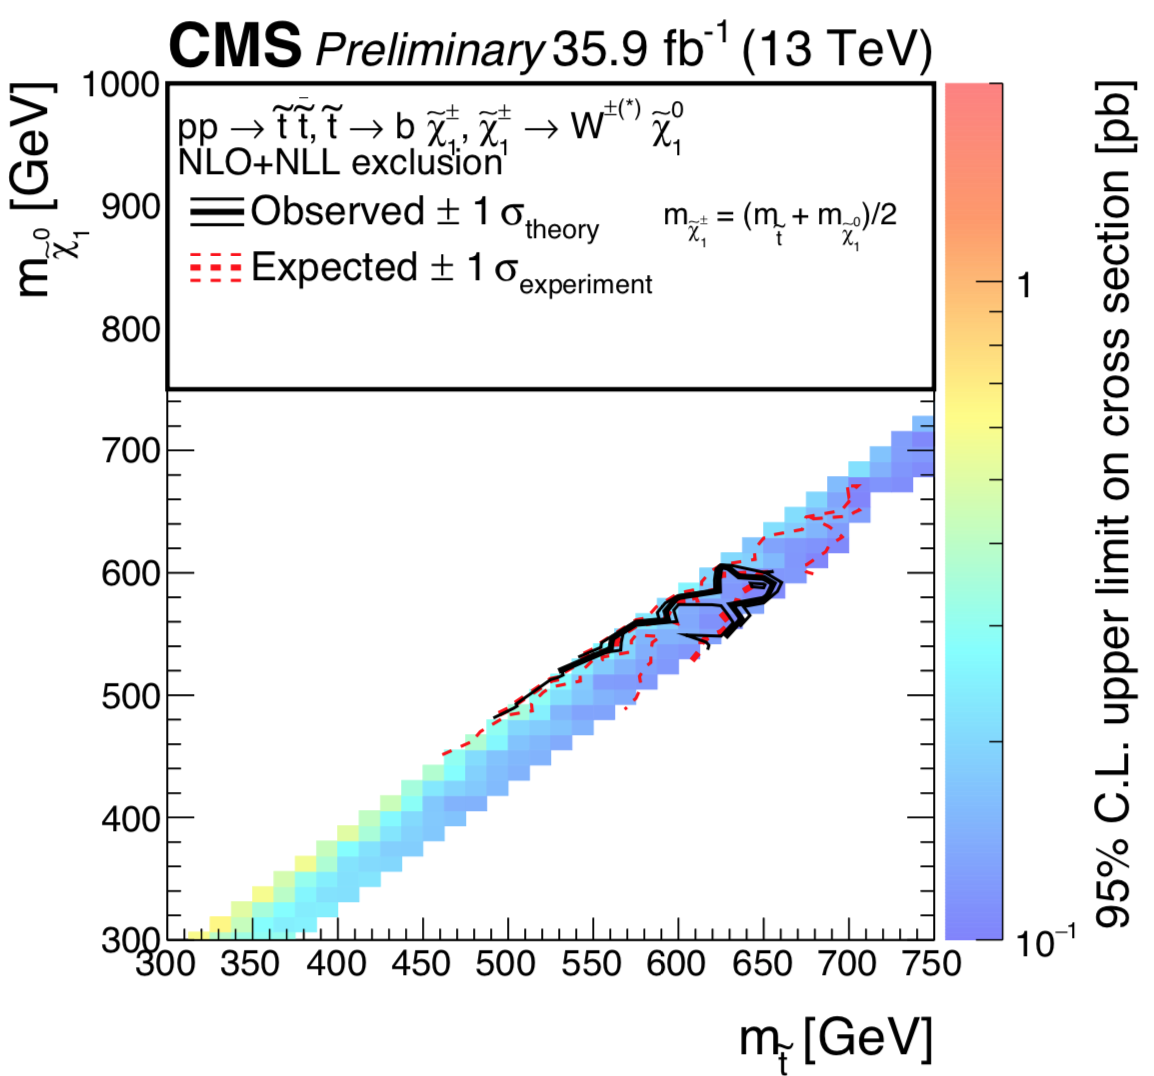
\includegraphics[width=0.50\textwidth]{T2bWC_AN16.png}
 	\caption[T2bWC Limits]{Limits for the mass parameter space for $\st\rightarrow b\chargino, \chargino\rightarrow W ^\pm\neutralino$ (T2bWC) decays. Which has a range of 550 to 675 \GeV{} for a \neutralino{} mass of 600 \GeV{} \cite{noauthor_search_nodate}.}
 	\label{T2bWCANLimits} 
\end{figure}

\begin{figure}
\centering
	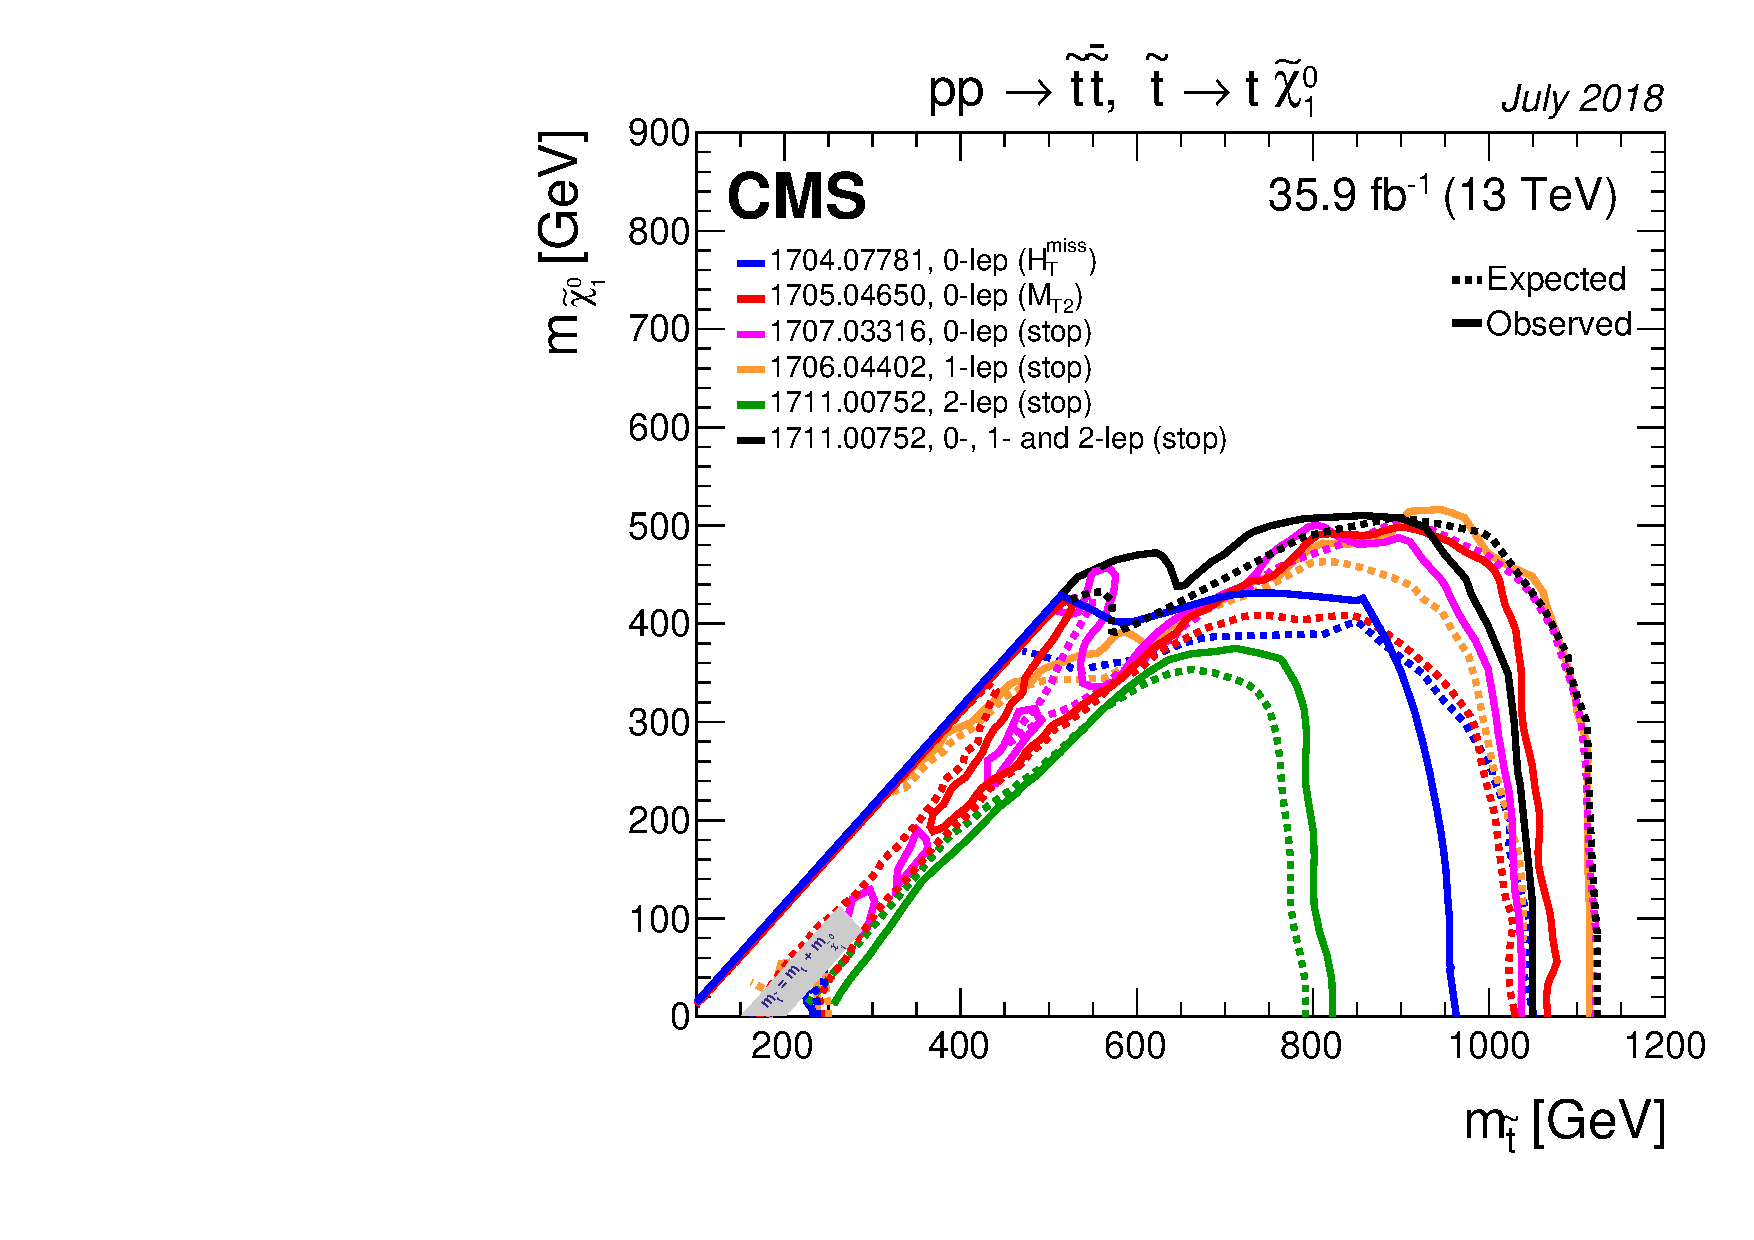
\includegraphics[width=0.50\textwidth]{T2tt_limits_summary_cms.pdf}
 	\caption[T2tt Limits for all decay modes]{Limits for the mass parameter space for T2tt decays using results from all the analysis in CMS. With a current limit of 800 GeV to 1.1 \TeV{} for a minimal neutralino mass.}
 	\label{T2ttCMSAll} 
\end{figure}

From the Fig. \ref{T2ttANLimits}, \ref{T2bWANLimits}, \ref{T2tbANLimits}, \ref{T2fbdANLimits}, \ref{T2bWCANLimits}, and \ref{T2ttCMSAll}, we know that we are able to exclude a large mass range for the \st{} and \neutralino{}. Since this is for a luminosity of 36.8 \fb, we can expect improved limits with all of the data from Run 2, which is 137 \fb. The new version of the analysis also has a redesigned search region to allow for more sensitive results, while also improving various object definitions.

\section{What are we looking for? And why?}
As discussed in Sec. \ref{sec:SM}, the SM is a robust theory that is useful for describing the iterations of visable matter in the universe. It has been through many robust tests, while also able to make many predictions. Unfortunately, we have seen that a few unknowns, such as: dark matter, the hierarchy problem, and a possible GUT, are currently unexplained. We then showed that a possible solution to these is SUSY, Sec. \ref{sec:SUSY}, which provides a good dark matter candidate, LSP, which allows for the convergence of the EM, Weak, and Strong force at large energy scales, and allows the Higgs mass to be renormalizable without fine tuning. 

From this, we have determined that the top squark is most likely to have the smallest squark mass in the MSSM. There have been many searches for the top squark decaying to many modes, which are summarized in Fig. \ref{T2ttCMSAll}. As of right now, we have set a limit on the \st{} mass, $m_{\st}>800$ GeV or $m_{\st}>1100$ GeV, depending on the analysis. Now we plan on using all of the data from Run2, 137 \fb, along with an improved search design to probe further into the mass parameter space of the \st{} and \neutralino{}.

\chapter{Compact Muon Solenoid}
\label{ch:CMS}

\section{The Detector}
\label{sec:cmsIntro}

The Compact Muon Solenoid (CMS) is a particle detector as part of the Large Hadron Collider (LHC) which is located near Geneva, Switzerland as part of the CERN collaboration. The CMS detector is 21.6 m long, 15 m diameter, and 14,000 tons and is used to detect many different species of particles. It is separated into layers that, from the interaction vertex outward are, the silicon tracker, Electromagnetic Calorimeter (ECAL), Hadronic Calorimeter (HCAL), superconducting solenoid, and the muon chambers, see Fig. \ref{CMSSlice}. 

\begin{figure}
 	\centering
	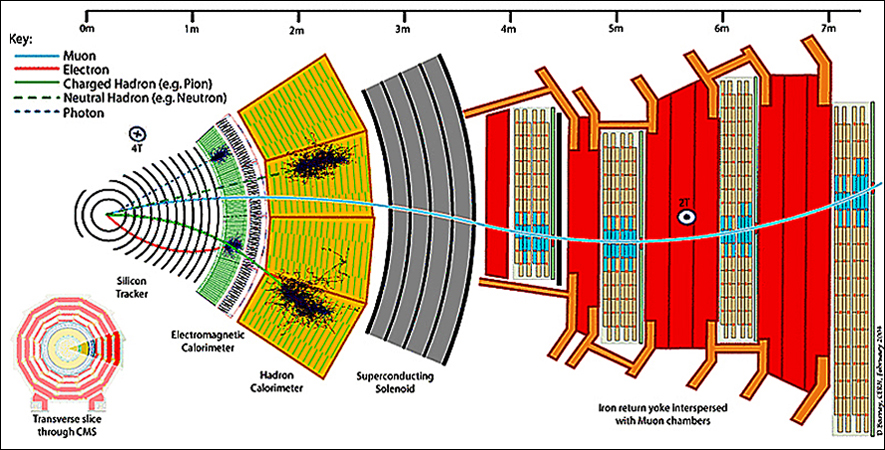
\includegraphics[width=0.75\textwidth]{cms_slice.jpg}
 	\caption[CMS Cross Section]{A cross-section of the CMS detector, oriented by looking down the direction of the beam pipe. }
 	\label{CMSSlice} 
\end{figure}

The CMS detector is designed to detect the decay products of most of the particles of the SM, except for neutrinos since they are weakly interacting and will almost certainly pass through the entire earth without an interaction. A defining feature of CMS is the 12.6-m long, 5.9 m inner diameter, 3.8 T superconducting solenoid. This is used to bend the trajectory of charged particles thoughout the detector, such that we can reconstruct the momentum and charge of the particles. The LHC provides a 13 TeV proton-proton beam (4.5 TeV heavy ion) beam with a bunch crossing every 25 ns (50 ns) to produce interaction at luminosities up to $2.5\times10^{34} \cm^{-2}s^{-1}$. 

The coordinate system of CMS has the origin at the nominal collision point in the center of the detector. The $y$-axis points vertically upward, $x$-axis points radially inward toward the center of the LHC, and $z$-axis points along the beam directions towards the Jura mountains from LHC Point 5. The polar angle $\theta$ is measured from the $z$-axis and the azimuthal angle $\phi$ is measured in the $x-y$ plane from the $x$-axis. The pseudorapidity of a particle is defined as $\eta=-\ln\tan(\theta/2)$ where $\theta$ is the angle between the particle momentum and the positive direction of the beam axis, two notable values are $\eta=0$ at $\theta=\pi/2$ and $\eta=\inf$ at $\theta=0$. Pseudorapidity is quite useful since the difference of pseudorapidities is Lorentz invariant. The transverse components of momentum, $p_T$, and energy, $E_T$, are computed using the $x$ and $y$ components of the particles. 

\subsection{Tracker}
\label{sec:Tracker}

The silicon tracker is made up of two different detectors, the silicon pixels and the silicon strip tracker. This is the inner most detector for CMS and receives the largest flux of particles during operation. This requires it to be radiation hard and operate with a fine granularity. 

\begin{figure}
 	\centering
	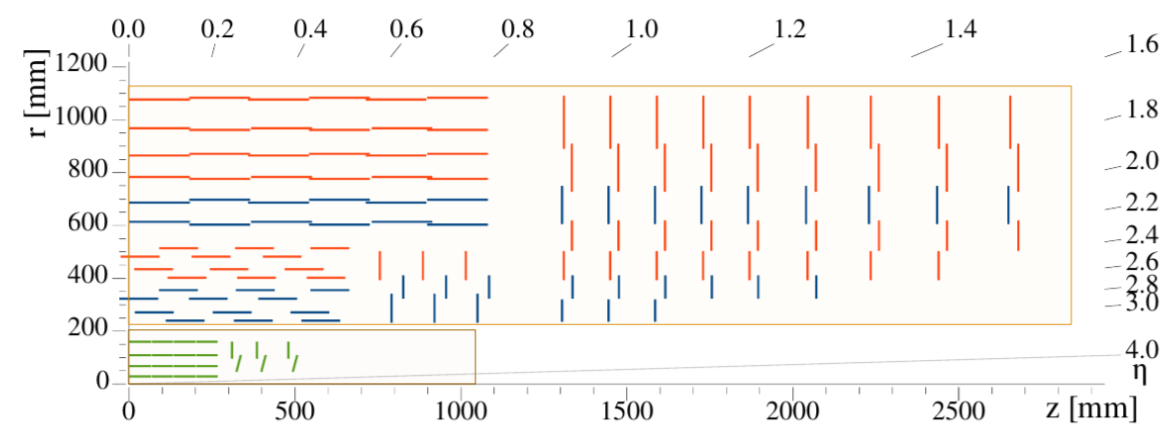
\includegraphics[width=0.75\textwidth]{Tracker_Configuration.png}
 	\caption[CMS Tracker Geometry]{Geometry of the CMS Tracker, the inner most region in green is the pixel detector while the outer region in blue and red are the silicon strips.}
 	\label{CMSTracker} 
\end{figure}

\subsubsection{Pixel Detector}
\label{subsec:Pixel}

The pixel detector was recently upgraded during the winter of 2016/2017. It is approximately 1 m long with four barrel layers ranging from 3.0, 6.8, 10.2, and 16.0 \cm{} from the beam axis and three endcap disks, see fig. \ref{CMSTracker}. Since it is the closest detector to the interaction vertex it therefore has the highest particle flux at $10^7/\cm^2/s$ at $r=10$ cm. The resolution is $9.4$ \mum{} in $r-\phi$ and $20-45$ \mum{} in $z$.

\begin{figure}
 	\centering
	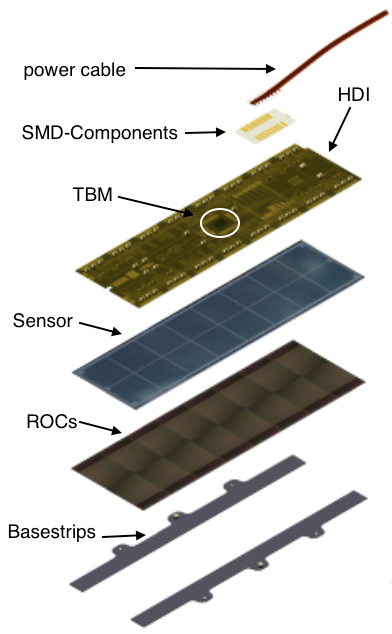
\includegraphics[width=0.5\textwidth]{Pixel_Module.png}
 	\caption[Pixel Modules]{Components of the pixel modules. Made up of a silicon layer, a grid of 8 ROCs which are attached via bump bonds. This is all controlled with a TBM connection to read out data.}
 	\label{PixelModule} 
\end{figure}

The pixel detector contains 1,184 modules in the barrel pixels (BPIX) and 672 modules in the forward pixels (FPIX). The number of individual pixels is 79 (45) million in the BPIX (FPIX) regions, respectively, with a pixel size of $100\times150 \text{ }\mum^2$. A pixel module contains two layers, a silicon layer that is bump bonded to 16 Readout Chips (ROCs) which form a module of 66560 pixels, see fig. \ref{PixelModule}. Each unit is controlled with one or more Token Bit Managers (TBMs) which controls the readout of the digital signal from the pixels to the Front-end Driver (FED). For BPIX Layers 3, 4 and all of FPIX there is 1 TBM per module. BPIX layer 2 has 2 TBMs with each one controlling 8 ROCs, while BPIX layer 1 has 4 TBMs with each one controlling 4 ROCs. The information from each module is split into two channels with each containing 8, 4, or 2 ROCs. These are encoded together by the TBM before being sent to the FED.

The silicon pixel system is set up as a reverse p-n junction, where the pixels are in the n-type region. As a charged particle travels through the silicon it creates electron-hole pairs. A voltage difference is applied to the silicon such that the electrons will deposit onto the pixels. Since the detector is inside of the magnetic field, a lorentz drift will cause the electrons to reach more than one pixel and increase the resolution. As the pixel system continues to be irradiated with large quantities of particles the voltage in the silicon decreases. This will lead to less charge sharing between the pixels and a decrease in resolution of particle locations. 

\begin{figure}
 	\centering
	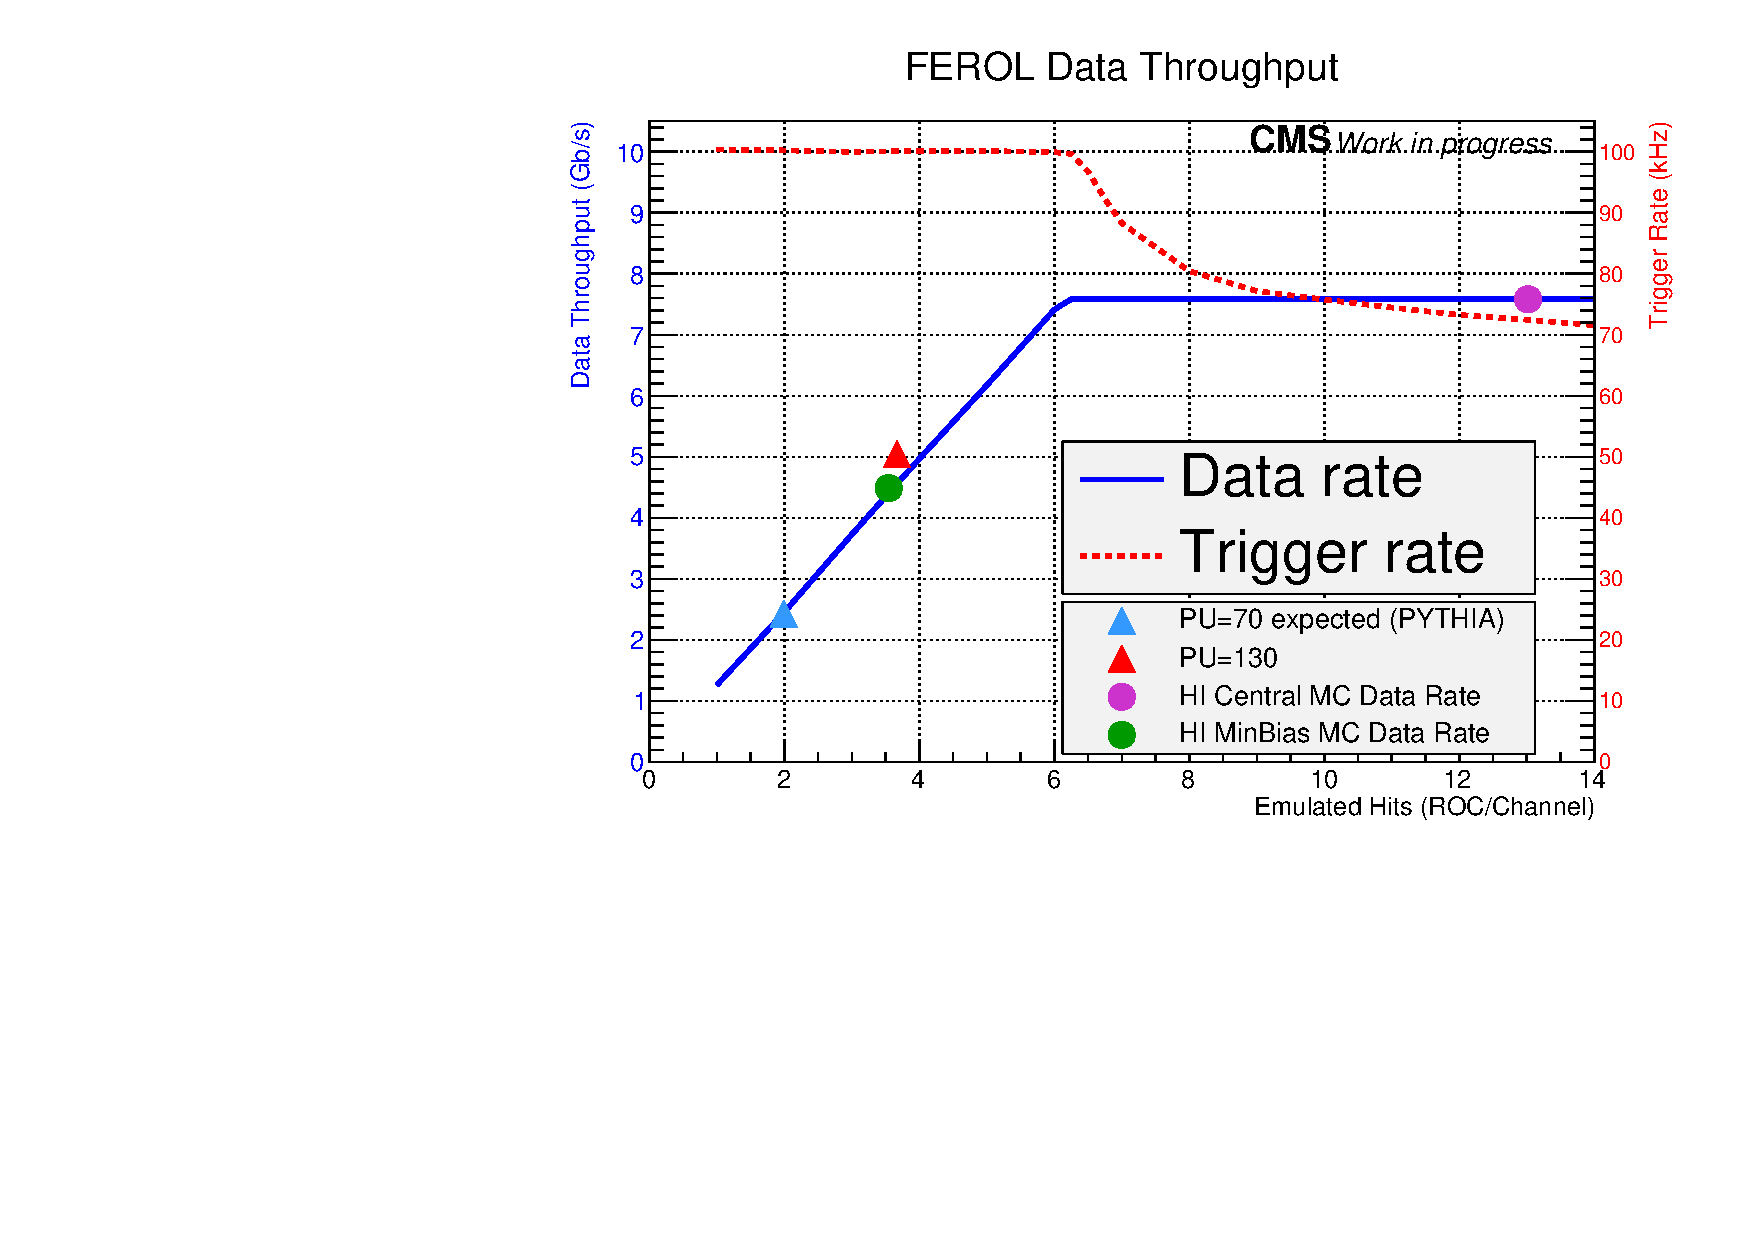
\includegraphics[width=0.75\textwidth]{FEROL_Data_Throughput_Thesis.pdf}
 	\caption[FED Throughput]{Measuring the throughput of the FED with the emulated and simulated events provided by the FED Tester. The Data rate is shown as the solid blue line with the corresponding trigger rate as the dotted red line. The simulated event sizes are shown as their equivalent emulated hits/ROC/channel on the data line.}
 	\label{FEDThroughput} 
\end{figure}

The data, from the pixels, is sent via optical fiber to the FED where is decoded and processes the information. The FED is responsible for identifying the relevant data, determining possible error states, and packaging the information to be sent to the central Data Acquisition (cDAQ) of CMS. Each of the 108 FEDs, for the pixels, receives 24 independent fibers from the detector. Each of these fibers contains 2 channels from the pixel module. Through robust testing with the FED Tester [Cite here], we have confirmed that the FED is able to attain a maximum data throughput of approximately 7.5 Gbps, see fig. \ref{FEDThroughput}. 

\subsubsection{Silicon Strips}
\label{subsec:Strips}

The silicon strips have a 200 m$^2$ active region with 15,148 modules that are distributed in 10 barrel layers and $9+3$ endcap disks.
This has a cell size ranging from $10 \text{ cm } \times80$ \mum{} to $25 \text{ cm } \times 180$ \mum{} since the particle flux decreases further away from the vertex, Fig. \ref{SiliconStrips}. It has a resolution of $23-24$ \mum{} in $r-\phi$ and $23$ \mum{} in $z$ for the microstrip tracker.

\begin{figure}[!htb]
	\centering
	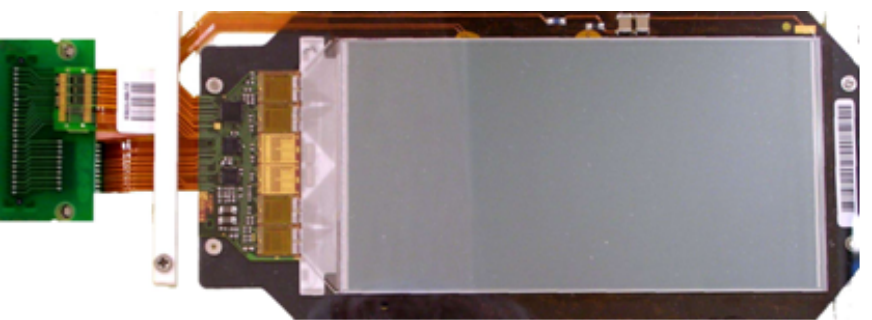
\includegraphics[width=0.75\textwidth]{StripTrackerModule.png}
	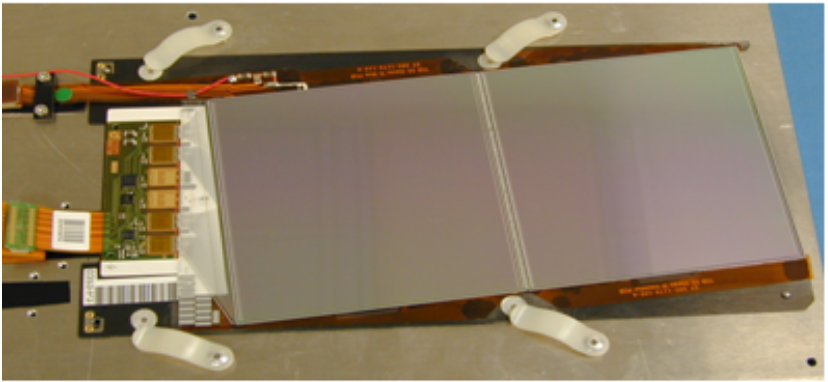
\includegraphics[width=0.75\textwidth]{StripTrackerModuleAngled.png}
	\caption[Strip Tracker Module]{The top module is a single sided reverse p-n silicon sensor. The bottom is two silicon sensors mounted back-to-back at a 100 mrad angle.}
 	\label{SiliconStrips} 
\end{figure}

There are two types of silicon strip module, see Fig. \ref{SiliconStrips}, which are in the layour shown in Fig. \ref{CMSTracker}. The orange modules are single sided reverse p-n silicon sensors, while the blue modules are double sided by having two single modules mounted back-to-back at a 100 mrad angle. This improves the 3D tracking, but unlike the pixel detector this is an analog readout system. 

\subsection{Electromagnetic Calorimeter}
\label{sec:ECAL}

The ECAL is a homogeneous calorimeter made out of 61,200 lead tungstate $(\text{PbWO}_4)$ crystals in the barrel and 7,324 crystals in each endcap. The barrel region has an inner radius of 129 cm and covers a pseudorapidity range of $0<|\eta|<1.479$. The encaps are 314 cm from the interaction point and cover a range $1.479<|\eta|<3.0$ in pseudorapidity. Lead tungstate was chosen for the crystals since it has a short radiation length, $X_0=0.89 \text{ cm }$, fast with 80\% of the light being emitted within 25 ns, and it's radiation hard. Each crystal in the barrel has a cross-section of $\approx22\times22 \text{ mm}^2$ and length of 230 mm, while the endcap crystals are $28.6\times28.6 \text{ mm}^2$ and length of 220 mm corresponding to $25.8X_0$ and $24.7X_0$, respectively. An ECAL uses electromagnetic showers to detect particles that interact electromagnetically. Electrons traveling through the material will radiate a photon via bremsstrahlung then the photon will pair produce two electrons. Combining these two processes leads to electromagnetic showers as the particles travel through the detector. The process will continue until a critical energy is reached such that an electron cannot radiate any further and will then lose energy via collisions. The hadrons that are created in the collisions will also interact in this way, but because of their large mass the penetrate through the entire ECAL. The resulting light is recorded by silicon avalanche photodiode (vaccuum phototriodes) in the barrel (endcap). 

\subsection{Hadronic Calorimeter}
\label{sec:HCAL}

The HCAL is a hermetic calorimeter consisting of alternating layers of brass as the absorber material and a scintillator. Brass is chosen since it is non-magnetic and has a relatively short interaction length. In the scintillator, a portion of the energy from the hadron in converted into visible light which is then measured by a hybrid photodiode tube to measure the energy. The barrel part of the HCAL consists of 2304 towers that are segmented into $\Delta\eta\times\Delta\phi=0.087\times0.087$ pieces that cover a region $0<|\eta|<1.4$ in pseudorapidity. The encap region consists of 2304 towers with varying segmentation sizes and a coverage of $1.3<|\eta|<3.0$. 

There are two additional parts of the HCAL to allow for maximum coverage of the detector volume. There is a outer hadron detector that is located outside the superconducting solenoid, which covers a slightly smaller pseudorapidity range as the barrel region. They serve as a tail catcher for hadron showers that penetrate all the way through the inner HCAL and solenoid. A forward hadron calorimeter, located 11.2 m from the interaction point covering a pseudorapidity $3.0<\eta<5.0$, made out of steel/quartz fiber is specifically designed for the columnated Cerenkov light in this region. 

\subsection{Superconducting solenoid}
\label{sec:Solenoid}

Surrounding most of this is the superconducting solenoid which is 12.6 m long with a 5.9 m radius. The field strength is 3.8 T which has a stored energy of approximately 2.7 GJ. The magnet is designed such that a muon with momentum, $p=1$ TeV, will have a momentum resolution of $\Delta p/p\approx10\%$. The solenoid is a high-purity aluminium-stabilized conductor, which is a similar material used in other large solenoids. 

\subsection{Muon Chambers}
\label{sec:muCham}

The muon system has three main detection systems that are used to identify a muon candidate. In the barrel region, drift tube (DT) chambers are used since the neutron background, muon rate, and magnetic field are all small. In the endcaps, cathode strip chambers (CSCs) are used since the relative values stated before are much larger. The neutron background is largely radially dependent so the CSCs will recieve a larger flux, while the muon rate is dominated by low $p_T$ muons which will interact in the endcap regions. Included throughout the whole system are resistive plate chambers (RPC). 

\begin{figure}
 	\centering
	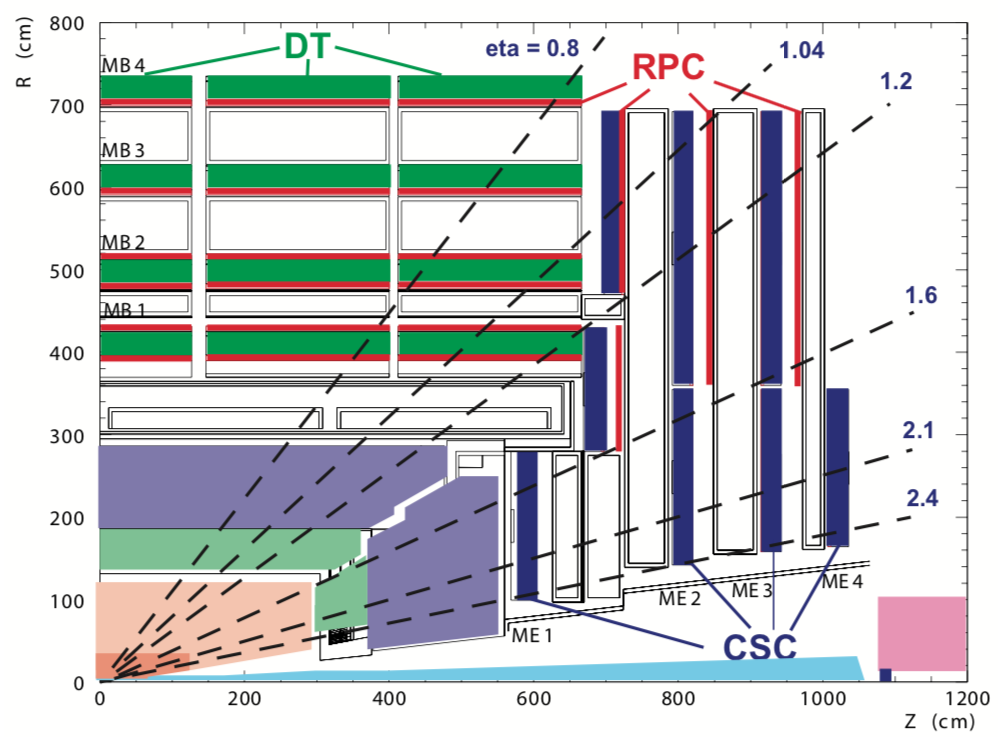
\includegraphics[width=0.75\textwidth]{MuonChambers.png}
 	\caption[Muon Chambers]{A quarter cross-section of the three muon detection systems for CMS. }
 	\label{MuonChambers} 
\end{figure}

The DT consists on 250 chambers in 4 barrel layers at a radii of 4.0, 4.9, 5.9, and 7.0 m from the beam axis. A DT chamber is an array of anode wires in a gaseous medium where the walls are cathodes. A muon passing through the gas will ionize some atoms which are then forced towards the anode wires by the electric field. The drift time of the electrons can then be calculated to within a couple of ns such that a good spatial resolution is achieved. The maximum designed drift length is 2.0 cm. Each station of the DT will give muon vector for each candidate with a $\phi$ precision of 100 \mum{} in postion and 1 mrad in direction. 

The CSC system uses the same concept as the DT system, but also includes a measurement of the ions that follow the electric field to the cathode strips. In this system the anode wires and the cathode strips are perpendicular so the collected charge on both provide a accurate position measurement. The RPC system contains two parallel plates, anode and cathode, the charge is measured by external metallic strips that can quickly measure the momentum of a muon and decide if the event should be triggered.

\section{Detector Methods}
\label{sec:DetMethods}

Using the objects and information from each of the subdetectors we can measure the important information required for doing innovative physics analysis, such as, the \st{} search. Since the search is dependent on large missing energies it is dependent on measuring all forms of energy in the standard model and checking for any inefficiencies. The CMS detector is designed to be an all encompassing detector to measure multiple processes in the SM and beyond. 
\chapter{Search Strategy}
\label{ch:SearchStrategy}

\section{Physics Objects}\label{PhysObj}
There are many different types of physics objects that we are interested in when working with particle physics experiments. Since the particles that we are interested in have very short lifetimes, $\mathcal{O}(\text{decay})=10^{-23}$ s, we mainly interact with the decay products of the event, such as, jets $(N_j)$, heavy object tagging $(\nt, \nw, \nrt)$, missing transverse momentum (\met), sum scalar jet momentum $(H_T)$, number of secondary vertices $(N_{SV})$, transverse momentum of leading $b$ jet $(\pt^b)$, transverse mass between tagged $b$ quarks amd \met{} $(m_T(b_{1,2}, \met))$, Initial State Radiation, and lepton identification.

\subsection{Jets}\label{Jets}
In an interaction whenever a quark is made it must come in pairs $(q\overline{q})$ such that the total color and electric charge of the interaction is neutral. Typically due to conservation of momentum the quarks may originally be produced near the interaction point but will quickly start to move away from each other. Eventually the quarks will move far enough apart and will have enough potential energy in the gluon connections between them that it is now more efficient to create a new quark-antiquark $(q\overline{q})$ pair. This will continue to occur in a sequence of radiating gluons and producing new pairs of charged particles. In the final state, the energy deposited in the HCAL is due to a cluster of charged particles of a certain radius, $\Delta R=\sqrt{\Delta\eta^2+\Delta\phi^2}$. There are many algorithms to reconstruct the jets, we are mainly interested in the anti-kT Jet algorithm \cite{cacciari_anti-ktjet_2008} method which uses the transverse momentum of the particles within a certain radius $\Delta R = 0.4 (0.8)$ for AK4(AK8) jets \cite{noauthor_jetid_nodate, noauthor_jec_nodate}. Once the jets have been identified, we cause analyse their respective properties to determine the likelihood of the particle it originated from, such as a $b, t, \text{ or } W$. 

\begin{figure}
 	\centering
	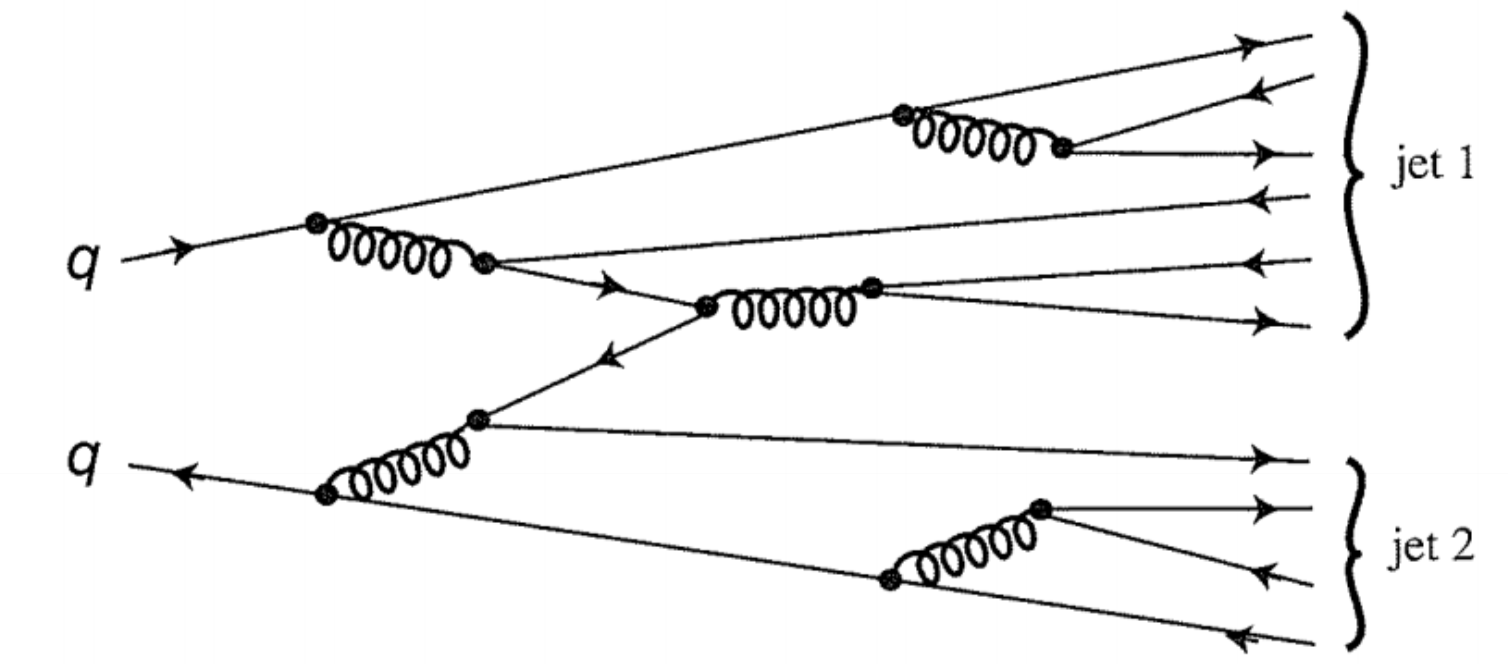
\includegraphics[width=0.75\textwidth]{JetHadronization.png}
 	\caption[Jet Hadronization]{A diagram of a quark pair radiating gluons that decay into more quark pairs in a process called hadronization \cite{griffiths_introduction_2008}.}
 	\label{JetHadronization} 
\end{figure}

\subsection{Heavy Object Tagging}\label{HeavyObject}
Since this search is looking for a massive particle which then decays to slightly less massive particles we need to be able to identify and distinguish between them. We use various algorithms and neural networks to identify jets from $b$ quarks, \bjet s or from $t$ quarks. 

\subsubsection{B-Tagging}\label{Btagging}
Firstly, \B-tagged jets which are jets that are likely to have originated from a \B{} quark. These are identified reconstructing where the jet originated from and comparing the distance away from the interaction point. A \B{} quark is a relatively long-lived particle and can travel many millimeters before decaying. Since we have a resolution of \mum{} this is not a problem. For \B{} quarks with large transverse momentum, we use a Deep Combined Secondary Vertex (DeepCSV) algorithm that involves neural networks. 

\bjet s{} are identified using the Run 2 version of the Deep Combined Secondary Vertex (DeepCSV) algorithm. The medium working point recommended by the B-tag POG, corresponding to a threshold of 0.6324m 0.4941, and 0.4184 for the 2016, 2017, and 2018 respectively \cite{noauthor_btagrecommendation2016legacy_nodate, noauthor_btagrecommendation94x_nodate, noauthor_btagrecommendation102x_nodate}.

\begin{figure}
 	\centering
	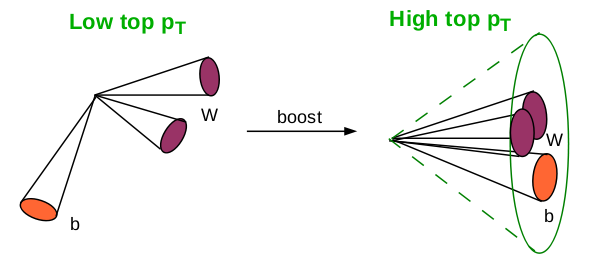
\includegraphics[width=0.75\textwidth]{TopDecayBoost.png}
 	\caption[Top Decays]{The two types of top quark reconstuctions, when each decay product is easily identifiable (resolved) or when the particles are close together (boosted).}
 	\label{TopDecays} 
\end{figure}

\subsubsection{Top/W Tagging}\label{TopTagging}
The anti-kt algorithm using a distance parameter, $\Delta R=0.8$, is expected to contain the energy clusters of all of the decay product of boosted $t$ quarks, see Fig. \ref{TopDecays}, with $\pt>300$ \GeV or \W bosons with $\pt>200$ \GeV. The requirements are:
\begin{itemize}
	\item Medium working point $>0.937, 0.895, 0.895 (0.973, 0.991, 0.991)$ for boosted $t$ $(W)$ for the separate 2016, 2017, and 2018 eras, respectively.
	\item Reconstructed soft drop mass: $105<m_t<210$ \GeV{} and $65<m_W<105$ \GeV.
	\item Boosted tops: $\pt=300$ \GeV, $|\eta|<2.0$ and $W$: $\pt=200$ \GeV, $|\eta|<2.0$
\end{itemize}

There is another type of top that can be reconstructed, which is when each subjet of the top decay can be resolved into each individual jet, denoted as a resolved top, see Fig. \ref{TopDecays}. The requirements are:
\begin{itemize}
	\item Medium working point: 0.92 for all eras.
	\item $|\eta(j_{1,2,3})|<2.4$ and $b$-tag desciminator: $>0.6324, 0.4941, 0.4184$ for the separate 2016, 2017, and 2018 eras, respectively. The number of jets that pass these cuts should be $\geq2$.
\end{itemize}
These object definition are orthogonal to each other and are used to bin our search and control regions. 

\subsection{Missing Transverse Momentum}\label{MET}
The missing transverse momentum is the negative vector sum of the total transverse momentum measured in the detector,
\begin{equation}
\met=-\sum_{i\in\text{vis}}\overrightarrow{p}_{i, T},
\end{equation}
where the momentum runs over every visible(vis) particle in the event. Ideally, if the detector was $100\%$ this quantity would always be zero due to conservation of momentum, but many things, such as detector efficiency, paticles that are weakly interacting, or particles beyond the SM will cause the missing energy. Because of these, this object is a good discriminator for searching for physics beyond the SM. 

\subsection{MET Filters}
Need to add MET Filters here.

\subsection{$H_T$}\label{HT}
Another interesting quantity is $H_T$, which is the scalar sum of the \pt of all of the jets in an event,
\begin{equation}
H_T=\sum_{i\in\text{jets}}p_{i,T}.
\end{equation}
This quantity is quite useful when trying to identify massive particles and is quite good at suppressing QCD multijet background.

\subsection{Soft $b$-Tagging}\label{SV}

The ability to identify secondary vertices is essential in searches for the top squark, see Sec. \ref{sec:Production}. Since the b quark is a long lived particle, about $10^{-12}$ seconds, that will travel many millimeters before decaying into other particles. The displaced vertex of the long lived $b$ quark is reconstructed from the tracks that it produces in the detector. We then reconstruct the tracks to a point that is displaced from the primary vertex $(PV)$ it is known as a secondary vertex $(SV)$ and has the potential to be an long lived particle. 

\begin{figure}
 	\centering
	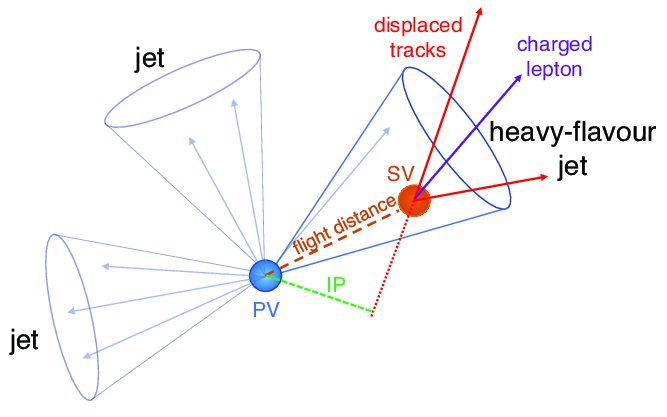
\includegraphics[width=0.75\textwidth]{SecondaryVertex.png}
 	\caption[Secondary Vertex Diagram]{A interaction that produces a long lived particle that has a reconstruced SV.}
 	\label{SecondaryVertex} 
\end{figure}

This search targets also models that produce very soft bottom or charm quarks. A large fraction of events contain b quarks with \pt{} below the 20 GeV jet \pt{} threshold which may thus fail to be reconstructed as jets or become b-tagged. Identification of these soft quarks improves our ability to separate potential signal events from the SM background. We therefore aim to identify b/c quarks based on the presence of a SV reconstructed using the Inclusive Vertex Finder (IVF) \cite{noauthor_inclusivesecondaryvertexfinder_nodate}. Additional requirements on SV observables are applied to suppress the background originating from light quarks. These selected SV may be referred to as soft $b$-tags and are constructed to be orthogonal to the jets and b-tagged jet used in this analysis. 

The requirements on each SV to pass the soft b-tagging definition are:
\begin{itemize}
	 \item The distance in the transverse plane between the SV and the PV $\leq3$ cm.
	 \item The significance of the distance, SIP3D, between the SV and thePV $\geq4$.
	 \item The pointing angle, defined as $cos(\overrightarrow{PV,SV},\overrightarrow{p}_{SV})\geq0.98$, where $\overrightarrow{p}_{SV}$ is the total four-momentum of the tracks associated to the SV. 
	 \item The number of tracks associated to the SV is greater or equal to 3.
	 \item The \pt{} of the SV is less than 20 GeV.
\end{itemize}

\subsection{Initial-state Radiation}\label{ISRpt}

Initial-state radiation (ISR) may be clustered into one of the large-$R$ jets clustered with a distance parameter, $\Delta R=0.8$. We use the larger radius jets to be sensitive to ISR with gluon splitting, when a jet radiates a qluon that pair produces two quarks. The ISR jet is identified as being the hardest of the large-$R$ jets with $\pt>200$ GeV which fails the loose b-tagging working point and is not identified as a top or W. 
 
 \subsection{Lepton Identification}\label{EleMuonID}
 There are two sets of selection criteria used in the analysis for electrons and muons. A set of veto criteria are used to efficiently reject events with an isolated electron of muon in the search region, while more stringent requirements are imposed in some control regions that require high purity samples of isolated leptons.
 
 Electron candidates are identified via a set of selection criteria established by the EGamma POG based on "Spring16" simulated samples in the 25ns bunch spacing scenario. The corresponding thresholds imposed on relevant variables are summarized in Table \ref{ElectronID}. The "Veto" working point is used to keep events with electrons out of the final search region. The "Medium" working point is used for the selection of leptonic control regions. 
 
 \begin{table}
 \centering
 \begin{tabular}{|*{5}{c|}}
 \hline
 \multirow{2}{*}{} & \multicolumn{2}{c}{Veto Working Point} & \multicolumn{2}{|c|}{Medium Working Point} \\
 \hline
 & Barrel & Endcap & Barrel & Endcap \\
\hline
$\sigma_{i\eta i \eta} (\text{full} 5 \times 5) <$ & 0.0114 & 0.0352 & 0.0101 & 0.0283 \\
$|\Delta\eta_{\text{in}}|<$ & 0.0152 & 0.0113 & 0.0103 & 0.00733 \\
$|\Delta\phi_{\text{in}}|<$ & 0.216 & 0.237 & 0.0336 & 0.114 \\
$\frac{h}{E} <$ & 0.181 & 0.116 & 0.0876 & 0.0678 \\
$\frac{1}{E}-\frac{1}{p}<$ & 0.207 & 0.174 & 0.0174 & 0.0898 \\
$|d_0|<$ & 0.0564 & 0.222 & 0.0118 & 0.0739 \\
$|d_z|<$ & 0.472 & 0.921 & 0.373 & 0.602 \\
$N(\text{expected missing inner hits})\leq$ & 2 & 3 & 2 & 1 \\
Conversion veto & pass & pass & pass & pass \\
\hline
 \end{tabular}
 \caption[Electron Identification Parameters]{Electron identification requirements, defined separately for electrons in the ECAL barrel and endcap regions. The tabulated numbers for each working point are the thresholds applied to the corresponding quantities in the first column. THESE NUMBERS NEED TO BE UPDATED!!!}
 \label{ElectronID}
 \end{table}
 
 The loose muon definition recommended by the Muon POG is used for the purposes of the muon veto. A loose muon is identified as a PF muon and can be either a global muon or an arbitrated tracker muon. Only candidates with transverse (longitudinal) impact parameter $|d_0|<0.2$ cm $(|d_z|<0.5 \text{cm},)$ with respect to the primary vertex, are considered. The muon selection in leptonic control regions relies on the medium working point defined by the Muon POG for higher purity. The medium muon requirements are summarized in Table \ref{MuonID}. They are applied in addition to the loose muon requirements. Selected muons are required to have transverse (longitudinal) impact parameters $|d_0|<0.05$ cm $(|d_z|<0.1 \text{cm}),$ with respect to the primary vertex. 

\begin{table}
 \centering
 \begin{tabular}{|*{2}{c|}}
 \hline
Loose muon selection & yes \\ 
Fraction of valid tracker hits & $> 0.8$ \\
\hline
\multicolumn{2}{|c|}{In addition, either of the following sets of requirements:} \\
\hline
Global muon & yes \\
Normalized global-track $\chi^2$ & $< 3$ \\
Tracker-Standalone position match & $< 12$ \\
Track kink finder & $< 20$ \\
Segment compatibility & $>0.303$ \\
\hline
\multicolumn{2}{|c|}{OR} \\
\hline
Segment compatibility & $> 0.451$ \\
\hline
 \end{tabular}
 \caption[Muon Identification Parameters]{The requirements for a particle trajectory to be tagged as a muon. THESE NUMBERS NEED TO BE UPDATED!!!}
 \label{MuonID}
 \end{table}
 
% The isolation requirements used in the selection of electrons and muons aim to achieve a high efficiency for correctly identifying events that contain prompt leptons (i.e. leptons that do not originate from heavy flavor decays) in the boosted topologies and busy hadronic environments that are typical for this analysis. They are based on the mini-isolation quantity, which is a measure of the lepton's local isolation. Mini-isolation is computed as the summed \pt of PF candidates within a $\Delta R$ cone centered on the lepton candidate. The cone size depends on the lepton \pt as indicated in Table  and is intended to be small enought to reduce overlaps with jets in the event while also being large enough to contain the products of leptonic b-decays. Higher values of instantaneous luminosity result in a reduced efficiency for the isolation requirement due to an increase in the number of particles originating from additional (pileup) interactions that enter the isolation cone. In order to minimize this effect, the calculated isolation quantity is corrected for the estimated contribution from pileup particles. The correction is applied by subtracting the product of the estimated average pileup density $(\rho)$ in the event with an effective area, $A_{eff}$, related to the geometrical size of the isolation cone. The residual dependence of the isolation quantity on $\rho$ for a given cone size is accounted for in $A_{eff}$, which is determined by taking the slope of a linear fit to the uncorrected isolation as a function of $\rho$. The correction factor is $\eta$-dependent, and calibrated separately for charged particles, neutral hadrons, and photons contributing to the isolation. 
 
 Electrons and muons are considered to fulfill the veto isolation criteria if their mini-isolation is less than 0.1 or 0.2 respectrively, relative to the lepton \pt. The same thresholds are applied on the relative mini-isolation for electrons and muons in control samples. 
 
\subsection{Tau Identification}\label{TauID}
The Tau ID has been studied extensively. After multiple studies which looked into the custum MVA \cite{roe_boosted_2004, hoecker_tmva_2007} similar to the one used in Ref. \cite{noauthor_search_nodate}, the cut-based IsoTrack method, and Tau POG MVA method of Identifying Taus. The methods which provide the best improvement to the efficiency of identifying taus with a small fake rate is the combination of IsoTrack and Tau POG MVA. With the inclusion of the combined method for identifying hadronically decaying taus, the veto percentage is $\approx29.0\%(7.2\%)$ with a efficiency of the veto efficiency of $\approx49.1\%(22.6\%)$ for SM background (signal), see Appendix. BLANK. 

\section{Search Strategy}\label{BaselineSearch}


\subsection{Trigger}
The following filters, recommended by the JetMET POG, are applied to 2016, 2017, and 2018 eras:
\begin{itemize}
	\item goodVertices
	\item HBHENoiseFilter
	\item HBHENoiseIsoFilter
	\item EcalDeadCellTriggerPrimitiveFilter
	\item BadPFMuonFilter
	\item GlobalSuperTightHalo2016Filter
	\item eeBadScFilter
\end{itemize}
There is an addition ecalBadCalibFilter for 2017 and 2018 eras only.

\subsection{Baseline Selection} \label{Baseline}

Following the same methods as above, we have a loose pre-selection which is refered to as the baseline selection. This will place a selection on jets and \met which is used to eliminate a large fraction of background events. We define the baseline selection as:
\begin{itemize}
	\item $N_{e,(\mu)} = 0, (\pt>5$ \GeV, $|\eta|<2.5(2.4), \text{miniISO}<0.1(0.2))$
	\item $N_{isoTrk} = 0, (\pt > 5 (10)$ \GeV, ISO $< 0.2(0.1) \text{ for electron/muons(pions)})$
	\item $N_{tauPOG} = 0, (\pt > 20$ \GeV, $|\eta|<2.4)$, medium working point
	\item $N_{j} \geq 2, (\pt >20$ \GeV, $|\eta|<2.4)$
	\item $\met >250$ \GeV, to reach the plateau of the trigger efficiency
	\item $\Ht>300$ \GeV
	\item HEM Veto for part of 2018 data: $-3\leq\eta\leq-1.4, -1.57\leq\phi\leq-0.87$
\end{itemize}
In Addition to this, we allow for two separte sets of additional selections to apply to the low and high \dm{} search regions to further reduce background. The high \dm{} baseline selection includes the baseline selection and additionally,
\begin{itemize}
	\item $N_j\geq 5, (\pt >20$ \GeV, $|\eta|<2.4)$
	\item $N_b\geq 1, (\pt >20$ \GeV, $|\eta|<2.4)$, medium DeepCSV
	\item $\text{Min}[|\Delta\phi(\met,j_1)|,|\Delta\phi(\met,j_2)|,|\Delta\phi(\met,j_3)|,|\Delta\phi(\met,j_4)|]\equiv\Delta\phi_{1234}>0.5$, where $j_1, j_2, j_3, j_4$ are the four leading jets in $p_T$. This requirement is to reduce the QCD multijet background. 
\end{itemize}
Next, the low \dm{} baseline selection has the following addition selections,
\begin{itemize}
	\item $N_t=0, N_W=0,N_{res}=0,$ where $N_t$ and $N_W$ are the number of merged tops and \W's, respectively, and $N_{res}$ is the number of resolved tops
	\item An ISR jet is defined in Sec. \ref{ISRpt} with $\pt(ISR)>200$ \GeV, $|\eta|<2.4, |\Delta\phi(j_{ISR},\met)|>2.$
	\item $\met/\sqrt{H_{T}}\equiv S_{\met}>10$, where $H_T$ is calculated as the scalar sum of the \pt of jets with $\pt >20$ \GeV{} and $|\eta|<2.4.$
	\item $|\Delta\phi(\met,j_1)|>0.5, |\Delta\phi(\met,j_{2,3})|>0.15$, where $j_1,j_2,j_3$ are the three leading jets in \pt. 
\end{itemize}
\begin{table}[!ht]
\begin{center}
\caption[High $\Delta$m Search Regions]{\label{tab:searchregions-hm}Summary of the 130 disjoint search regions that mainly target high \dm~signal models. The high \dm~baseline selection is again $\nj \geq 5$, $\met>250~\GeV$, $\nb\geq1$, and $\dphijonetwothreefour>0.5$.}
\resizebox*{1\textwidth}{!}{

\begin{tabular}{|c|c|c|c|c|c|c|}
	\hline
	\multicolumn{7}{|c|}{$\mtb<175$\,\GeV}  \\
	\hline
	\nj				 & \nb				& \nt			   & \nw				 & \nrt				& \Ht ~[\GeV]		   & \met~[\GeV] 		\\
	\hline
	$\geq7$		& $1, \geq2$  & $\geq0$		 & $\geq0$			& $\geq1$	  & $\geq300$			& $250-300$, $300-400$, $400-500$, $\geq500$ \\
	\hline
	\multicolumn{7}{|c|}{$\mtb\geq175$\,\GeV}  \\
	\hline
	\nj				 & \nb				& \nt			   & \nw				 & \nrt				& \Ht ~[\GeV]		   & \met~[\GeV] 		\\
	\hline
	$\geq5$		& $1,\geq2$   &	$0$				& $0$				   & $0$			 & $\geq1000$		 & $250-350$, $350-450$, $450-550$, $\geq550$ \\
	\hline
	\multirow{6}{*}{$\geq5$} & \multirow{6}{*}{$1$} & $\geq1$ & $0$ & $0$ & $300-1000$, $1000-1500$, $\geq1500$ & $250-550$, $550-650$, $\geq650$\\
						  &					   & $0$			 & $\geq1$			& $0$			  & $300-1300$, $\geq1300$ & $250-350$, $350-450$, $\geq450$ \\
						  &					   & $0$			 & $0$				    & $\geq1$	  & $300-1000$, $1000-1500$, $\geq1500$ & $250-350$, $350-450$, $450-550$, $550-650$, $\geq650$ \\
						  &					   & $\geq1$	 & $\geq1$			& $0$			  & $\geq300$ 			& $250-550$, $\geq550$ \\
						  &					   & $\geq1$	 & $0$					& $\geq1$	  & $\geq300$			& $250-550$, $\geq550$ \\
						  &					   & $0$			 & $\geq1$			& $\geq1$	  & $\geq300$			& $250-550$, $\geq550$ \\
	\hline
	\multirow{10}{*}{$\geq5$} & \multirow{10}{*}{$2$} & $1$ & $0$ & $0$ & $300-1000$, $1000-1500$, $\geq1500$ & $250-550$, $550-650$, $\geq650$\\
						  &					   & $0$			 & $1$					& $0$			& $300-1300$, $\geq1300$ & $250-350$, $350-450$, $\geq450$ \\
						  &					   & $0$			 & $0$				    & $1$	  		& $300-1000$, $1000-1500$, $\geq1500$ & $250-350$, $350-450$, $450-550$, $550-650$, $\geq650$ \\
						  &					   & $1$	 		 & $1$					& $0$			& $\geq300$ 						& $250-550$, $\geq550$ \\
						  &					   & $1$	 		 & $0$					& $1$	  		& $300-1300$, $\geq1300$ & $250-350$, $350-450$, $\geq450$ \\
						  &					   & $0$			 & $1$					& $1$	  		& $\geq300$							& $250-550$, $\geq550$ \\
						  &					   & $2$	 		 & $0$					& $0$			& $\geq300$ 						& $250-450$, $\geq450$ \\
						  &					   & $0$	 		 & $2$					& $0$	  		& $\geq300$ 						& $\geq250$ \\
						  &					   & $0$			 & $0$					& $2$	  		& $300-1300$, $\geq1300$ & $250-450$, $\geq450$ \\
						  &					   & \multicolumn{3}{|c|}{$\nt+\nw+\nrt\geq3$} & $\geq300$ 					   & $\geq250$ \\
	\hline
	\multirow{10}{*}{$\geq5$} & \multirow{10}{*}{$\geq3$} & $1$ & $0$ & $0$ & $300-1000$, $1000-1500$, $\geq1500$ & $250-350$, $350-550$, $\geq550$\\
						  &					   & $0$			 & $1$					& $0$			& $\geq300$ 						& $250-350$, $350-550$, $\geq550$\\
						  &					   & $0$			 & $0$				    & $1$	  		& $300-1000$, $1000-1500$, $\geq1500$ & $250-350$, $350-550$, $\geq550$\\
						  &					   & $1$	 		 & $1$					& $0$			& $\geq300$ 						& $\geq250$ \\
						  &					   & $1$	 		 & $0$					& $1$	  		& $\geq300$ 						& $250-350$, $\geq350$ \\
						  &					   & $0$			 & $1$					& $1$	  		& $\geq300$							& $\geq250$ \\
						  &					   & $2$	 		 & $0$					& $0$			& $\geq300$ 						& $\geq250$ \\
						  &					   & $0$	 		 & $2$					& $0$	  		& $\geq300$ 						& $\geq250$ \\
						  &					   & $0$			 & $0$					& $2$	  		& $\geq300$ 					   & $250-350$, $\geq350$ \\
						  &					   & \multicolumn{3}{|c|}{$\nt+\nw+\nrt\geq3$} & $\geq300$ 					   & $\geq250$ \\
	\hline
\end{tabular}
}
\end{center}
\end{table}

\begin{table}[!ht]
\begin{center}
\caption[Low $\Delta$m Search Regions]{\label{tab:searchregions-lm}Summary of the 53 disjoint search regions that mainly target low \dm~signal models. The low \dm~baseline selection is again $\nj \geq 2$, $\met>250~\GeV$, $\nt=\nw=\nrt=0$, $\nb\geq0$, $\mtb<175~\GeV$ (when applicable), $|\Delta\phi(\text {j}_1,\met)|>0.5, ~~ |\Delta\phi(\text {j}_{2,3},\met)| > 0.15$, $\pt(ISR) > 200$~\GeV, $ |\eta(ISR)| < 2.4$, $|\Delta\phi(j_{\text{ISR}},\met)|>2$, and $\metsig > 10$.}
\resizebox*{1\textwidth}{!}{
\begin{tabular}{|c|c|c|c|c|c|}
	\hline
	$\nj$              & $\nb$                    & $\nsv$             & $\ptisr$~[\GeV]         & $\ptb$~[\GeV]      & $\met$~[\GeV]                           \\
	\hline
	$2-5$              & \multirow{4}{*}{0}       & 0                  & \multirow{4}{*}{$>500$} & \multirow{4}{*}{-} & $450-550$, $550-650$, $650-750$, $>750$ \\
	$\geq6$            &                          & 0                  &                         &                    & $450-550$, $550-650$, $650-750$, $>750$ \\
	$2-5$              &                          & $\geq1$            &                         &                    & $450-550$, $550-650$, $650-750$, $>750$ \\
	$\geq6$            &                          & $\geq1$            &                         &                    & $450-550$, $550-650$, $650-750$, $>750$ \\
	\hline
	\multirow{5}{*}{$\geq2$} & \multirow{5}{*}{1}   & 0                  & $300-500$               & $20-40$            & $300-400$, $400-500$, $500-600$, $>600$ \\
	&                          & 0                  & $300-500$               & $40-70$            & $300-400$, $400-500$, $500-600$, $>600$ \\
	&                          & 0                  & $>500$                  & $20-40$            & $450-550$, $550-650$, $650-750$, $>750$ \\
	&                          & 0                  & $>500$                  & $40-70$            & $450-550$, $550-650$, $650-750$, $>750$ \\
	&                          & $\geq1$            & $>300$                  & $20-40$            & $300-400$, $400-500$, $>500$            \\
	\hline
	$\geq2$            & \multirow{6}{*}{$\geq2$} & \multirow{6}{*}{$\geq0$} & $300-500$               & $40-80$            & $300-400$, $400-500$, $>500$            \\
	$\geq2$            &                          &                          & $300-500$               & $80-140$           & $300-400$, $400-500$, $>500$            \\
	$\geq7$            &                          &                          & $300-500$               & $>140$             & $300-400$, $400-500$, $>500$            \\
	$\geq2$            &                          &                          & $>500$                  & $40-80$            & $450-550$, $550-650$, $>650$            \\
	$\geq2$            &                          &                          & $>500$                  & $80-140$           & $450-550$, $550-650$, $>650$            \\
	$\geq7$            &                          &                          & $>300$                  & $>140$             & $450-550$, $550-650$, $>650$         \\
	\hline
\end{tabular}
}
\end{center}
\end{table}



\section{Search Regions}


\chapter{Top Squark Production and Backgrounds}
\label{ch:Search}

We have now motivated that the top squark, \st{}, could be the lightest squark, see Sec. \ref{subsec:StopMassSpec}. This allows us to possibly produce them at CMS. In Sec. \ref{sec:Baseline}, we have designed a search that will look for events with large amounts of \met{} and \nj. These events are being targeted in separate low \dm{} and high \dm{} search regions. For all of these we are interested in comparing the data and background in each search or control region. We will look at the production and decay modes of various \st{} interactions and the estimation of the SM background of each region. 

\section{Production and Decay Modes}
\label{sec:Production}

To produce the top squark all we need is the collision of two proton-proton beams. It is shown as a black circle in the Fig. \ref{fig:stop-gluino-production} and \ref{fig:stop-direct-production}. This is meant to represent many processes that can make a top squark. The main processes are gluon fusion, when two gluons fuse into a single gluon which then decays into a top and anti-top squark pair, or annihilation, where two quarks annihilate to a gluon propagator which thus decays into two top squarks. 

\begin{figure}[!h]
	\begin{center}
		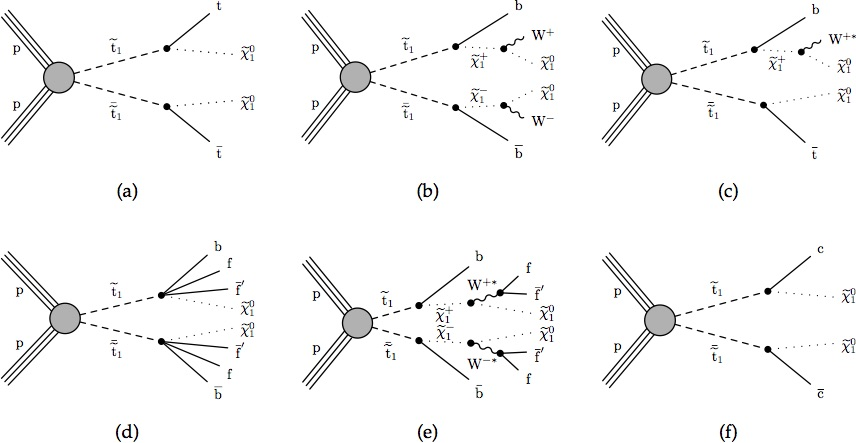
\includegraphics[width=1.00\textwidth]{T2tt_all.jpg}
	\end{center}
	\caption[Direct stop production]{Feynman diagrams for the direct \st{} production in SUSY. The allowed decay modes are (a) T2tt, (b) T2bW, (c) T2tb, (d,e) T2fbd, and (f) T2cc. }
	\label{fig:stop-direct-production}
\end{figure}

\begin{figure}[!h]
	\begin{center}
		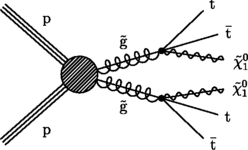
\includegraphics[width=0.32\textwidth]{T1tttt.png}
		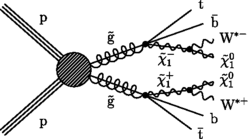
\includegraphics[width=0.32\textwidth]{T1ttbb.png} \\
		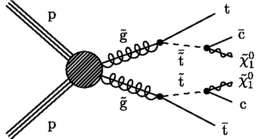
\includegraphics[width=0.32\textwidth]{T5ttcc.png}
		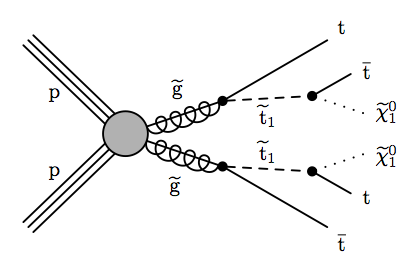
\includegraphics[width=0.32\textwidth]{T5tttt.png} \\
	\end{center}
	\caption[Gluino mediated stop production]{Feynman diagrams for the indirect \st{} production in SUSY. The allowed decay modes are T1tttt (top left), T1ttbb (top right), T5ttcc (bottom left), and T5tttt (bottom right).
	}
	\label{fig:stop-gluino-production}
\end{figure}


The main decay mode of the top squark is $\st\rightarrow t+\neutralino$ and $\st\rightarrow b+\chargino$, Fig. \ref{fig:stop-direct-production}. The top quark most likely decays as, $t\rightarrow b\W^+$, while the $b$ quark will decay to either a $c$ or an $u$ quark in its decay chain with an additional \W{} boson. The \neutralino{} is proposed to be a stable dark matter candidate while the \chargino{} could decay as, $\chargino\rightarrow\neutralino\W$. Next, a four body decay is allowed for, $\st\rightarrow b f f^\prime \neutralino$, see Fig. \ref{fig:stop-direct-production}(d,e). The final direct \st{} production we are interested in is the $\st\rightarrow c\neutralino$, see Fig. \ref{fig:stop-direct-production}(f). To be as inclusive as possible, we are also including indirect top squark production as see in Fig. \ref{fig:stop-gluino-production}. We see that the \st{} will decay to multiple jets, \nj, and missing transverse energy, \met. Now we are going to try to estimate the SM background that could be in each of our search region bins.

\section{Standard Model Background}
\label{sec:SMBackground}

The standard model background for the top squark search is defined by a large \met{} and a multiple jets. The are a couple types of SM background that can be misinterpreted as our signal. The most likely background is that which causes many tops (or heavy particles) and missing energy. Events in the SM like \ttbar{} and \W+jets will have many jets produced and \met{} due to a missed lepton and neutrino. The production of heavy particles like \Znunu{} will give multiple jets and \met{} from the neutrinos being missed by the detector. QCD events often produce events with multiple jets, due to acceptances in the detector the jets can sometimes be mis-measured which can cause large \met{}. There are also various processes that are quite rare which are quite rare but still need to be accounted for. 

\section{Lost Lepton}
\label{sec:LL}

The contribution from the \ttbar{} and \W+jets processes arises from leptonic decays of the \W{} boson, where the charged lepton is outside the kinematic acceptance of CMS or evades identification by the dedicated lepton vetoes. Large \met{} can be generated by the associated neutrino and the lepton that is not reconstructed, allowing such events to enter the search regions. This background is collectively referred to as the "Lost Lepton" (LL) background. Contributions arising from $tW, ttW$ and single-top processes also enter into this category, but with much smaller importance. 

Studies in simulation indicate that the event kinematics for different lepton flavors are similar enough to allow us to estimate them collectively from a single control sample in data that has event characteristics similar to those of the search sample. Because of this, we use the single-lepton control sample to estimate the LL background, using the method described in detail in Ref. \cite{bravo_search_2015}. The single-lepton sample consists of events that have one lepton satisfying the lepton-veto criteria. In order to suppress potential signal contamination, we require $M_T(l,\met)<100~\GeV$. The requirement of low $M_T(l,\met)$ also ensures orthogonality to the search regions used in direct top squark production in the single-lepton or double-lepton final state, making it possible to statistically combine the results of the two searches. The selection applied to the single-lepton control sample follows the same selection on the search variables as in the zero-lepton selection with the exception of classification according to the number of top and \W-tagged candidates. 

\subsection{Combining All Run 2 Eras}\label{sec:LLCombination}
Firstly, for this analysis we are interested in the possibility in combining the yields of each era into one estimation. This is initially done by looking at the \met{} distributions in each era. Since the LL estimation is done with the transfer factor method, a good confirmation would be the comparison of the transfer factor in each SR for each era. 
\begin{figure}[!htb]
	\begin{center}
  \includegraphics[width=0.32\textwidth]{../Research/SUSY/2019/LLB/njets20_v3/MET_pt_DataMC___llcr_lm_RunBtoE_2017_allPU.pdf}
  \includegraphics[width=0.32\textwidth]{../Research/SUSY/2019/LLB/njets20_v3/MET_pt_DataMC___llcr_lm_RunF_2017_allPU.pdf} \\
  \includegraphics[width=0.32\textwidth]{../Research/SUSY/2019/LLB/njets20_v3/MET_pt_DataMC___llcr_lm_PreHEM_2018_allPU.pdf}
  \includegraphics[width=0.32\textwidth]{../Research/SUSY/2019/LLB/njets20_v3/MET_pt_DataMC___llcr_lm_PostHEM_2018_allPU.pdf} \\
	\end{center}
	\caption{Comparison of the Data and MC in the 1Lep CR for each era: Run2016, Run2017BtoE, Run2017F, Run2018preHEM, Run2018PostHEM, and the combination of all eras in the Low \dm{} region. Each era has a good agreement between Data and MC. 
	 }
	\label{fig:llb-1lcr-datavsmc-lm-inclusive}
\end{figure}
\begin{figure}[!htb]
	\begin{center}  
		\includegraphics[width=0.32\textwidth]{../Research/SUSY/2019/LLB/njets20_v3/MET_pt_DataMC___llcr_hm_RunBtoE_2017_allPU.pdf}
		\includegraphics[width=0.32\textwidth]{../Research/SUSY/2019/LLB/njets20_v3/MET_pt_DataMC___llcr_hm_RunF_2017_allPU.pdf} \\
		\includegraphics[width=0.32\textwidth]{../Research/SUSY/2019/LLB/njets20_v3/MET_pt_DataMC___llcr_hm_PreHEM_2018_allPU.pdf}
		\includegraphics[width=0.32\textwidth]{../Research/SUSY/2019/LLB/njets20_v3/MET_pt_DataMC___llcr_hm_PostHEM_2018_allPU.pdf}
	\end{center}
	\caption{Comparison of the Data and MC in the 1Lep CR for each era: Run2016, Run2017BtoE, Run2017F, Run2018preHEM, Run2018PostHEM, and the combination of all eras in the High \dm{} region. Each era has a good agreement between Data and MC. 
	 }
	\label{fig:llb-1lcr-datavsmc-hm-inclusive}
\end{figure}


\subsection{Transfer Factors}
\label{subsec:TF}

The LL estimation in each search region is based upon the event count in data in the corresponding control region in the single-lepton sample. The count is extrapolated to the search region to obtain a prediction by means of a transfer factor obtained from simulation as follows: 

\begin{equation}
\label{eqn:LLTF}
N_{pred}^{LL}=TF_{LL} \cdot N_{data}(1l).
\end{equation}

This allows us to have the same selection for the single-lepton control sample and the zero-lepton sample. The only exception is the number of top and W-tagged candidates. The LL estimation is dependent on the yield of data in the corresponding CR and the TF calculated by the single-lepton sample. The transfer factor is defined as, 
\begin{equation}
\label{eqn:TF}
TF_{LL}=\frac{N_{MC}(0l)}{N_{MC}(1l)},
\end{equation}
where $N_{MC}(1l)$ is the event count observed in the corresponding CR and $N_{MC}(0l)$ use the event count in the corresponding SR. 

The main motivation behind this approach is to increase the statistical precision of the background estimation. The performance of the $t$ and \W{} taggers has been studied in data and MC samples and a reasonably good agreement is observed allowing us to proceed with this approach. Data-to-MC scale factors are extracted and applied to MC to account for residual differences of the tagging performance in data. Detailed studies comparing the performance of the $t$ and \W{} taggers in data and MC \cite{noauthor_search_nodate}.

The control regions utilized to predict the LL background are displayed in Fig. \ref{fig:llb-1lcr-datavsmc-lm-nb0} to \ref{fig:llb-1lcr-datavsmc-hm-nb3-1}. The figures \ref{fig:llb-1lcr-datavsmc-lm-nb0} to \ref{fig:llb-1lcr-datavsmc-lm-nb1} display the control regions specific to the low \dm{} selection, where the regions are binned following the search region definition. Figures \ref{fig:llb-1lcr-datavsmc-hm-nt0-nrt0-nw0} to \ref{fig:llb-1lcr-datavsmc-hm-nb3-1} display the control regions dedicated for the high \dm{} selection. Due to the nature of the background estimation method applied in the high \dm{} search, control regions are utilized for the prediction of multiple search regions. 

Tables \ref{tab:0l-llb-pred-lm} to \ref{tab:0l-llb-pred-hm-3} summarize the yields in data observed in the single-lepton sample, the derived transfer factor, and the resulting LL predictions for the low \dm{} and high \dm{} search regions respectively. The transfer factors in the high \dm{} region actually account for two levels of extrapolation. The CR for the high \dm{} is loose such that, there is no binning in tops or W tagging. We then extrapolate to the SR with the inclusion of the top and W tags, along with scale factors, to estimate the LL background in the region:
\begin{equation}\label{TFExtrapolation}
\begin{split}
TF_{LL}=& TF_{LL}^{CR-SR}\times TF_{LL}^{SR-extrap} \\
=& \frac{N_{MC}(0l)(\nj,\nb,\met)}{N_{MC}(1l)(\nj,\nb,\met)}\times\frac{N_{MC}(0l)(\nj,\nb,\met,\nt,\nrt,\nw)}{N_{MC}(0l)(\nj,\nb,\met)}.
\end{split}
\end{equation}

We now want to consider how the transfer factor for each era relates to the total transfer factor. In Fig. \ref{fig:llb-1lcr-datavsmc-total-tf} and \ref{fig:llb-1lcr-datavsmc-sep-tf}, we see the comparison the the total $TF$ for each era of the data and simulation. these are all in quite good agreement, but we see are large peak near zero. Once we alter the comparison for the $TF$ for the CR-to-SR and the SR-to-Extrapolation. We see a much better agreement when we do not include the cuts on top/W tagging. These are improved because of the better statistics in the region. 
\begin{figure}
	\begin{center}
  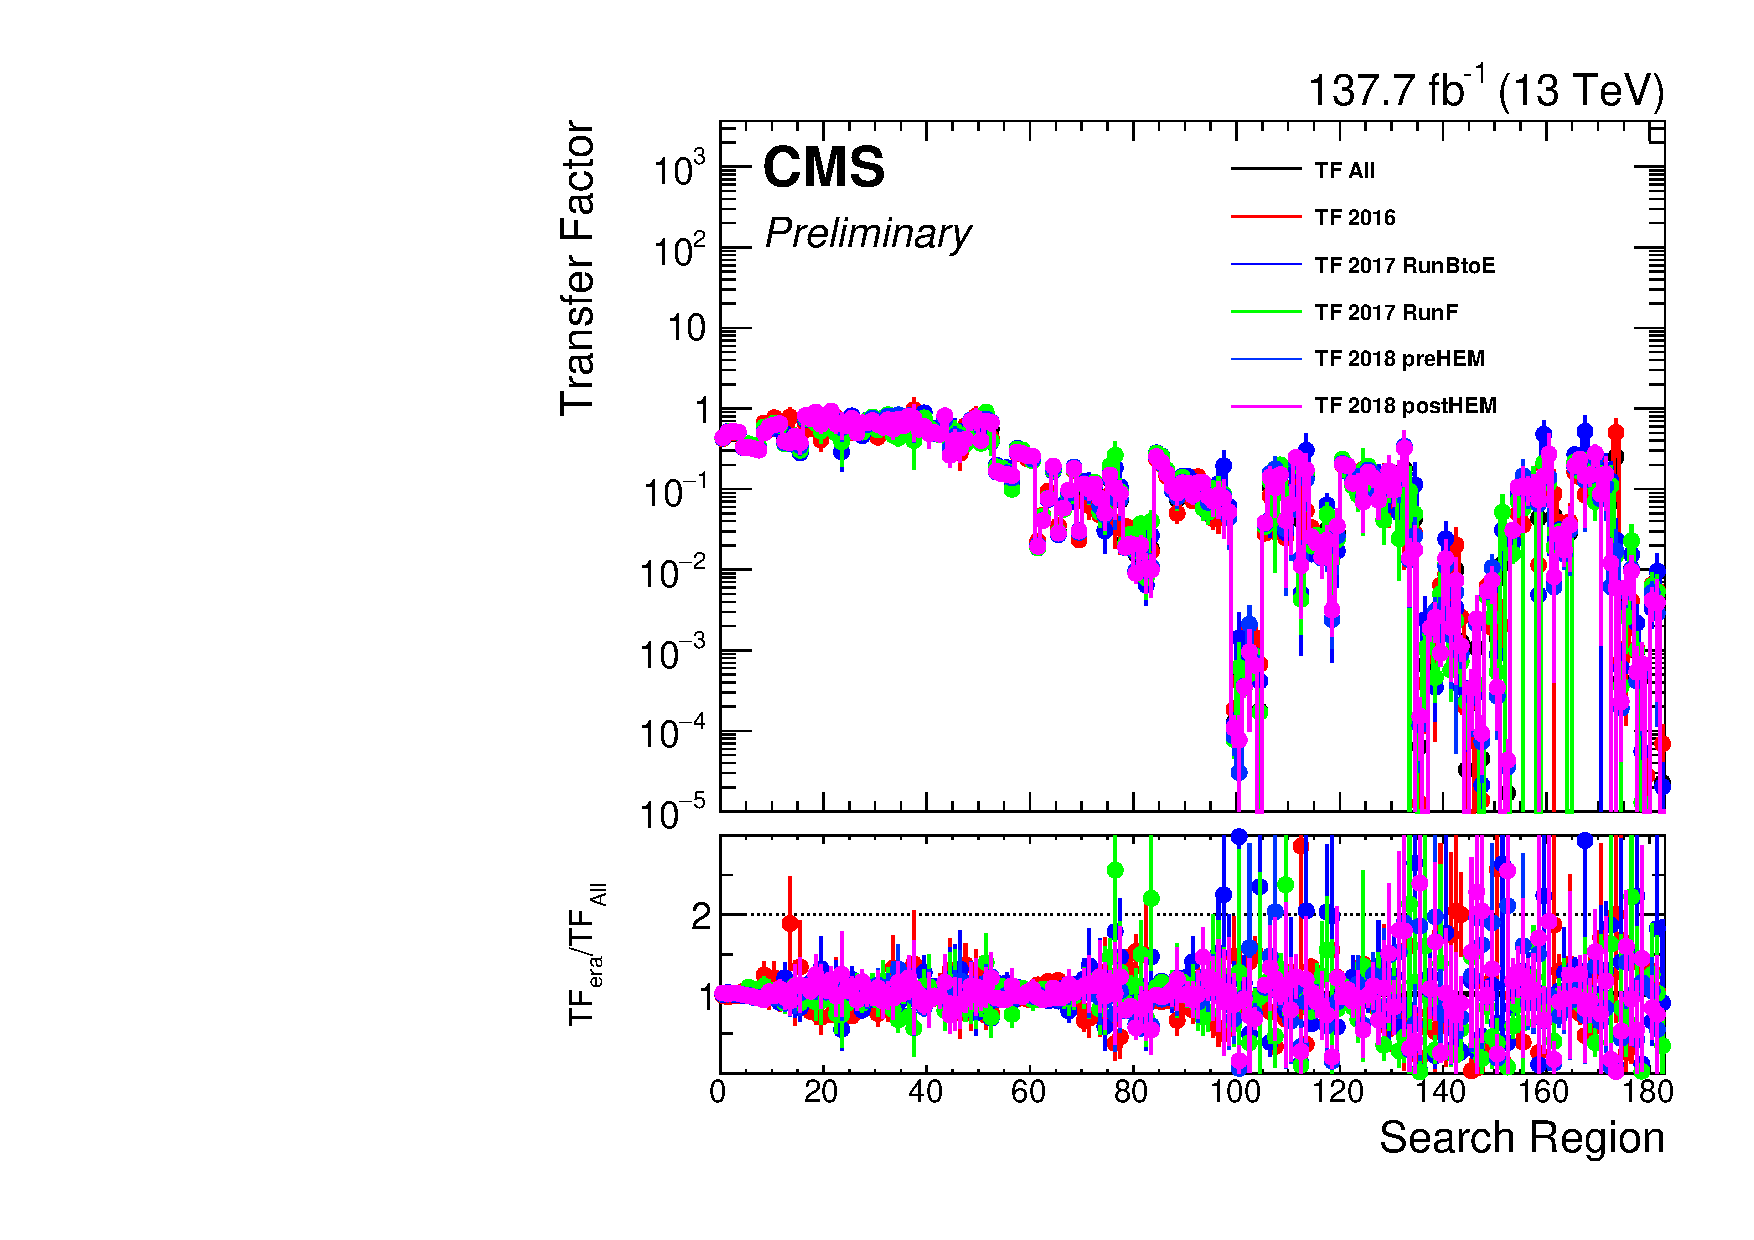
\includegraphics[width=0.4\textwidth]{LostLepton_TF_Comparison.pdf}
  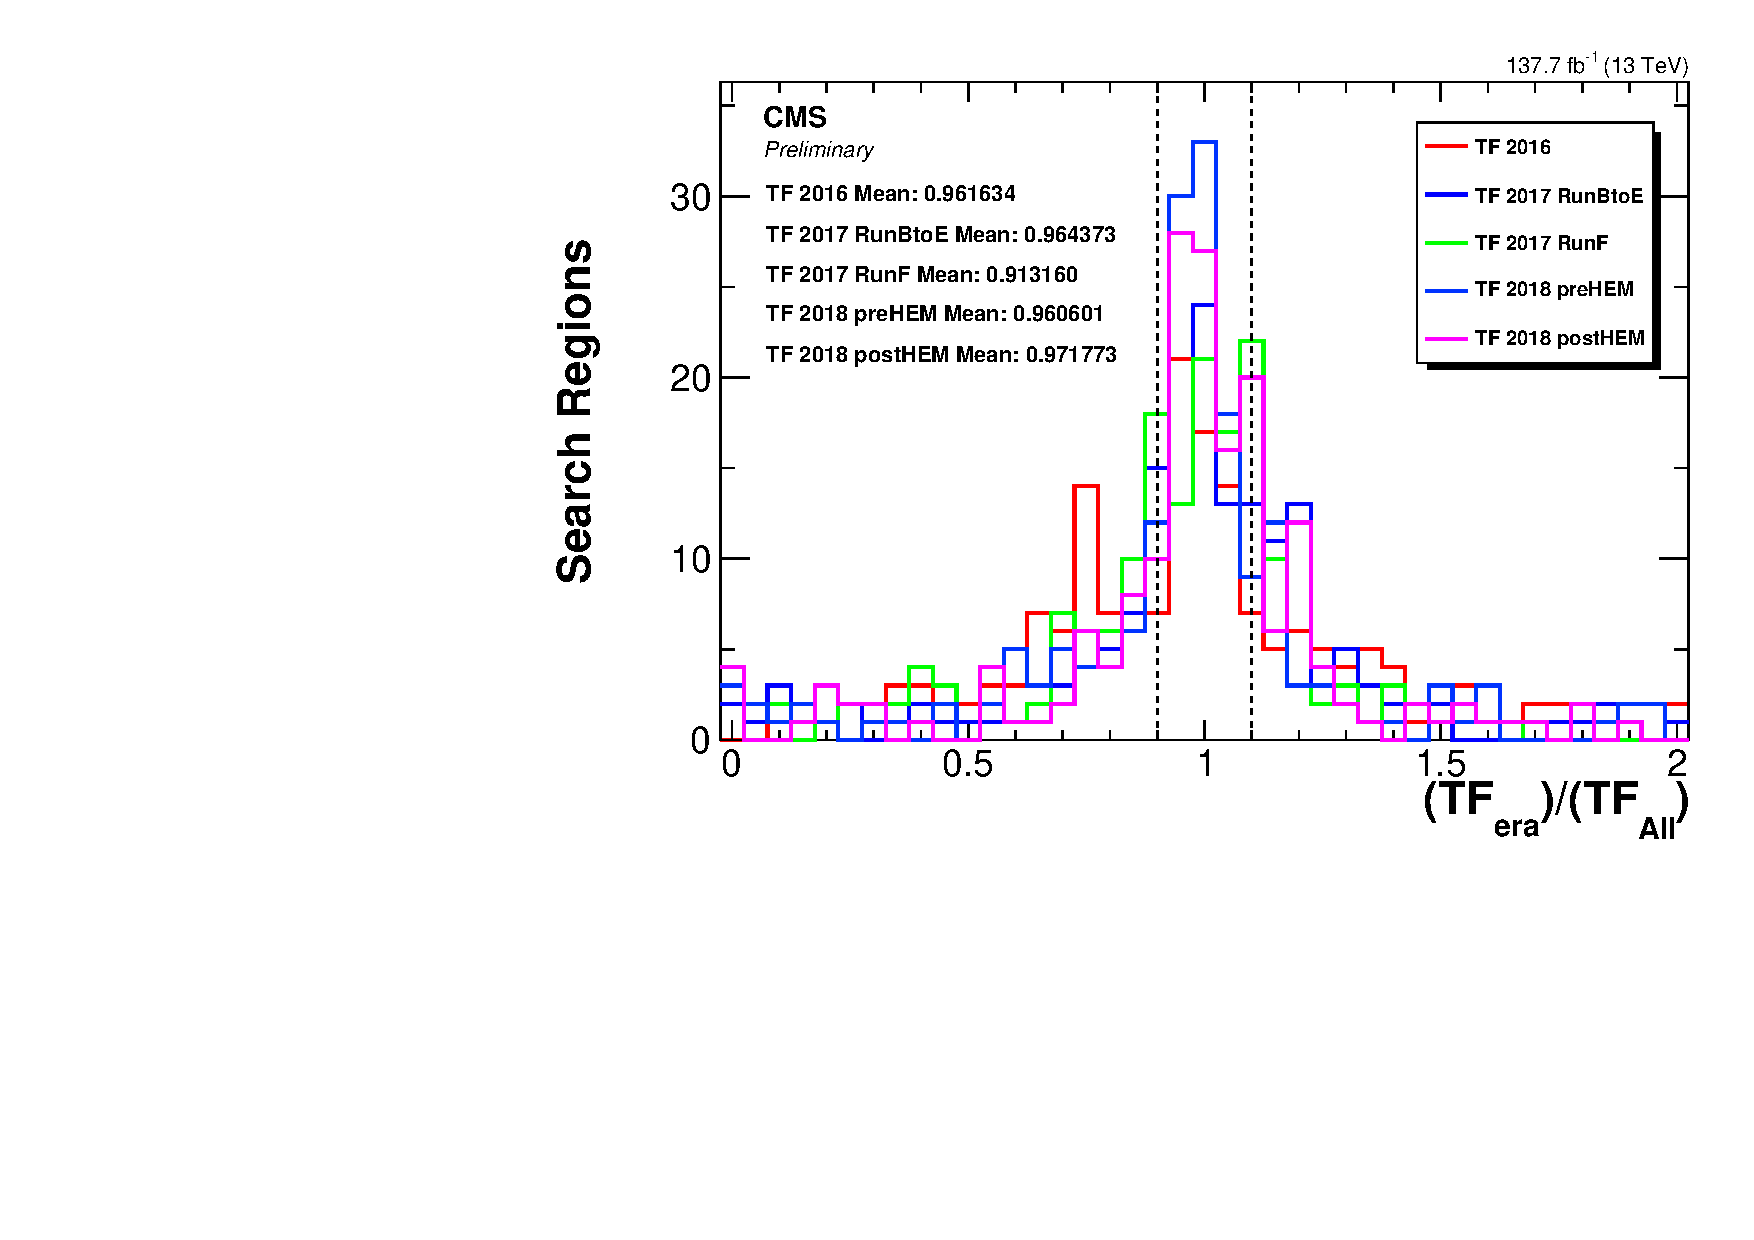
\includegraphics[width=0.5\textwidth]{LostLepton_TF_Comparison_sum.pdf} \\
	\end{center}
	\caption[Transfer Factor Comparison]{Comparisons of the transfer factors for each era of MC in the low and high \dm{} regions. The values are shown in their separate bins on the left plot and in a combined form on the right. The mean for each is also shown. 
	 }
	\label{fig:llb-1lcr-datavsmc-total-tf}
\end{figure}
\begin{figure}
	\begin{center}  
		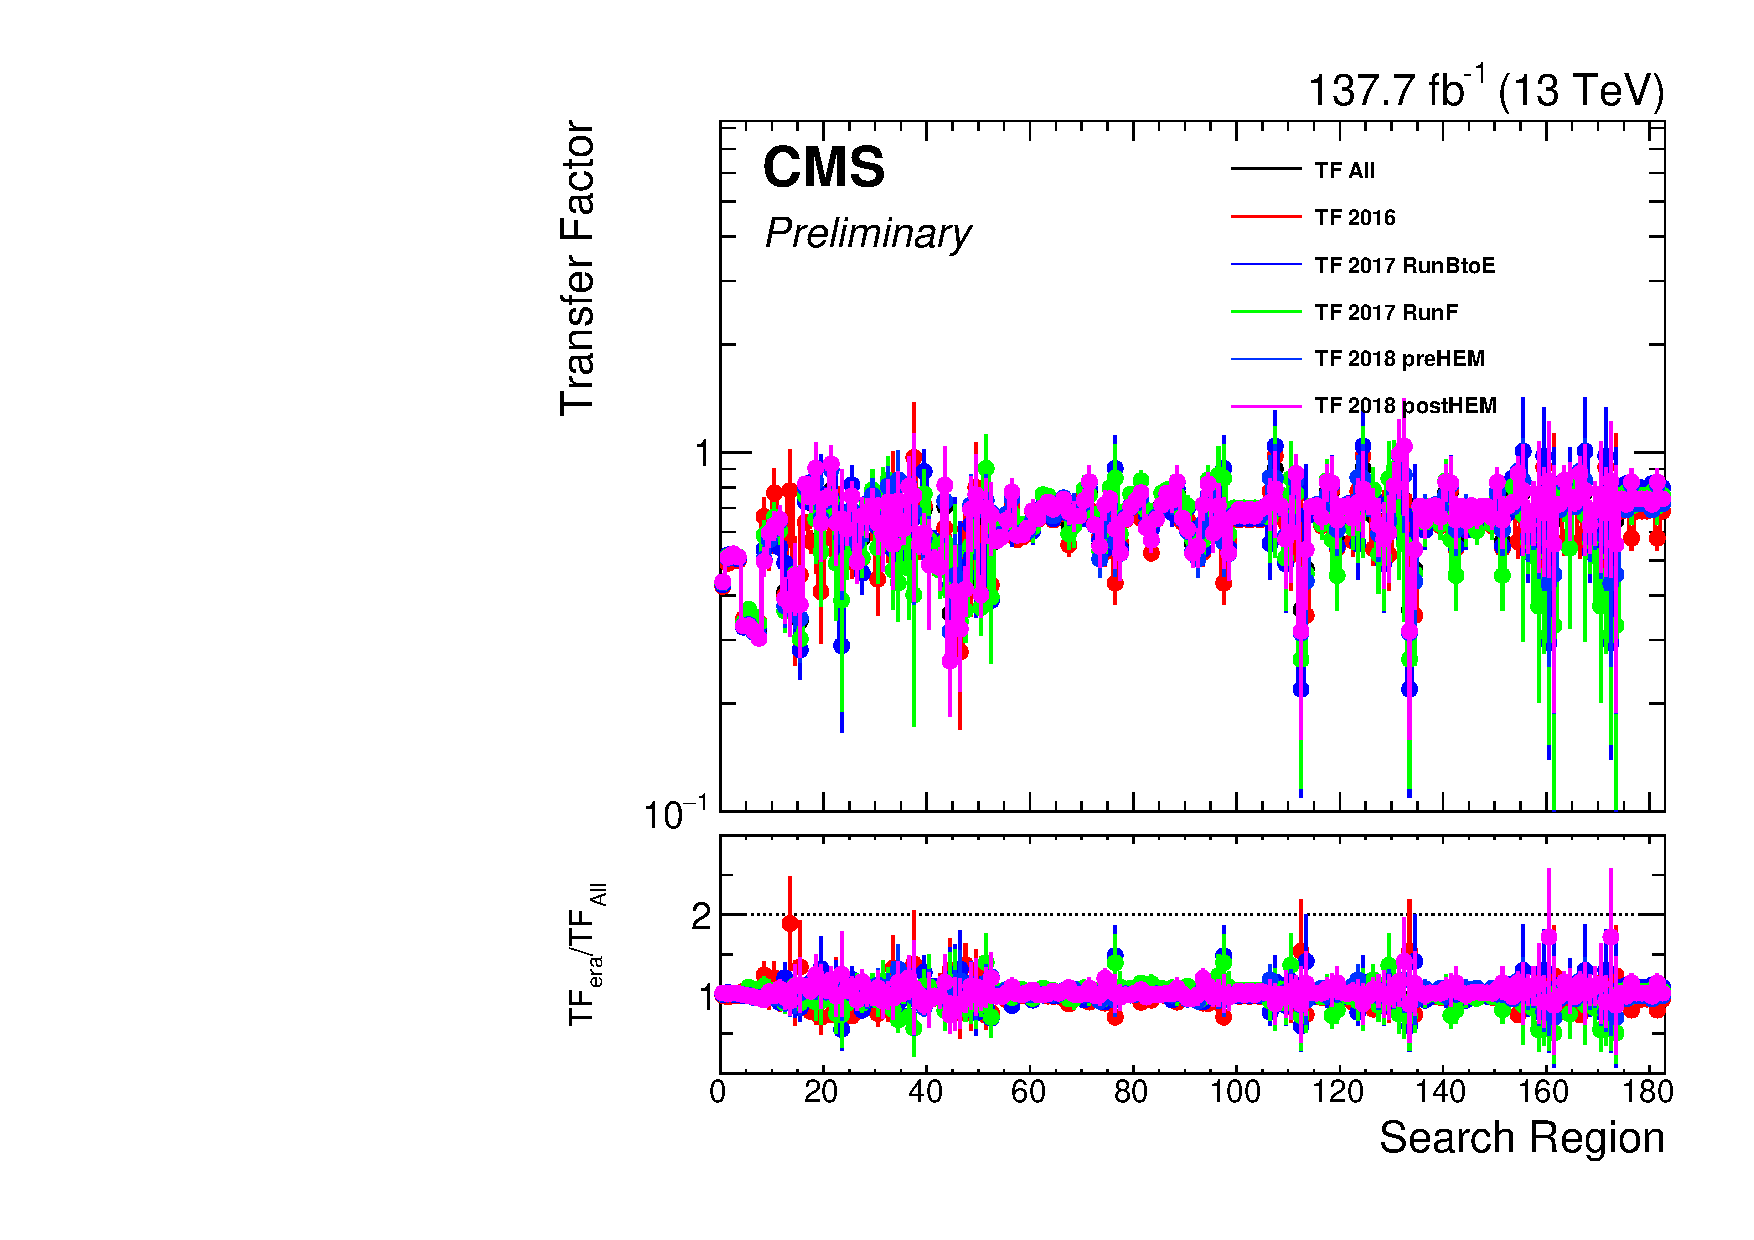
\includegraphics[width=0.4\textwidth]{LostLepton_TF_CR_to_SR_noextrap_Comparison.pdf}
		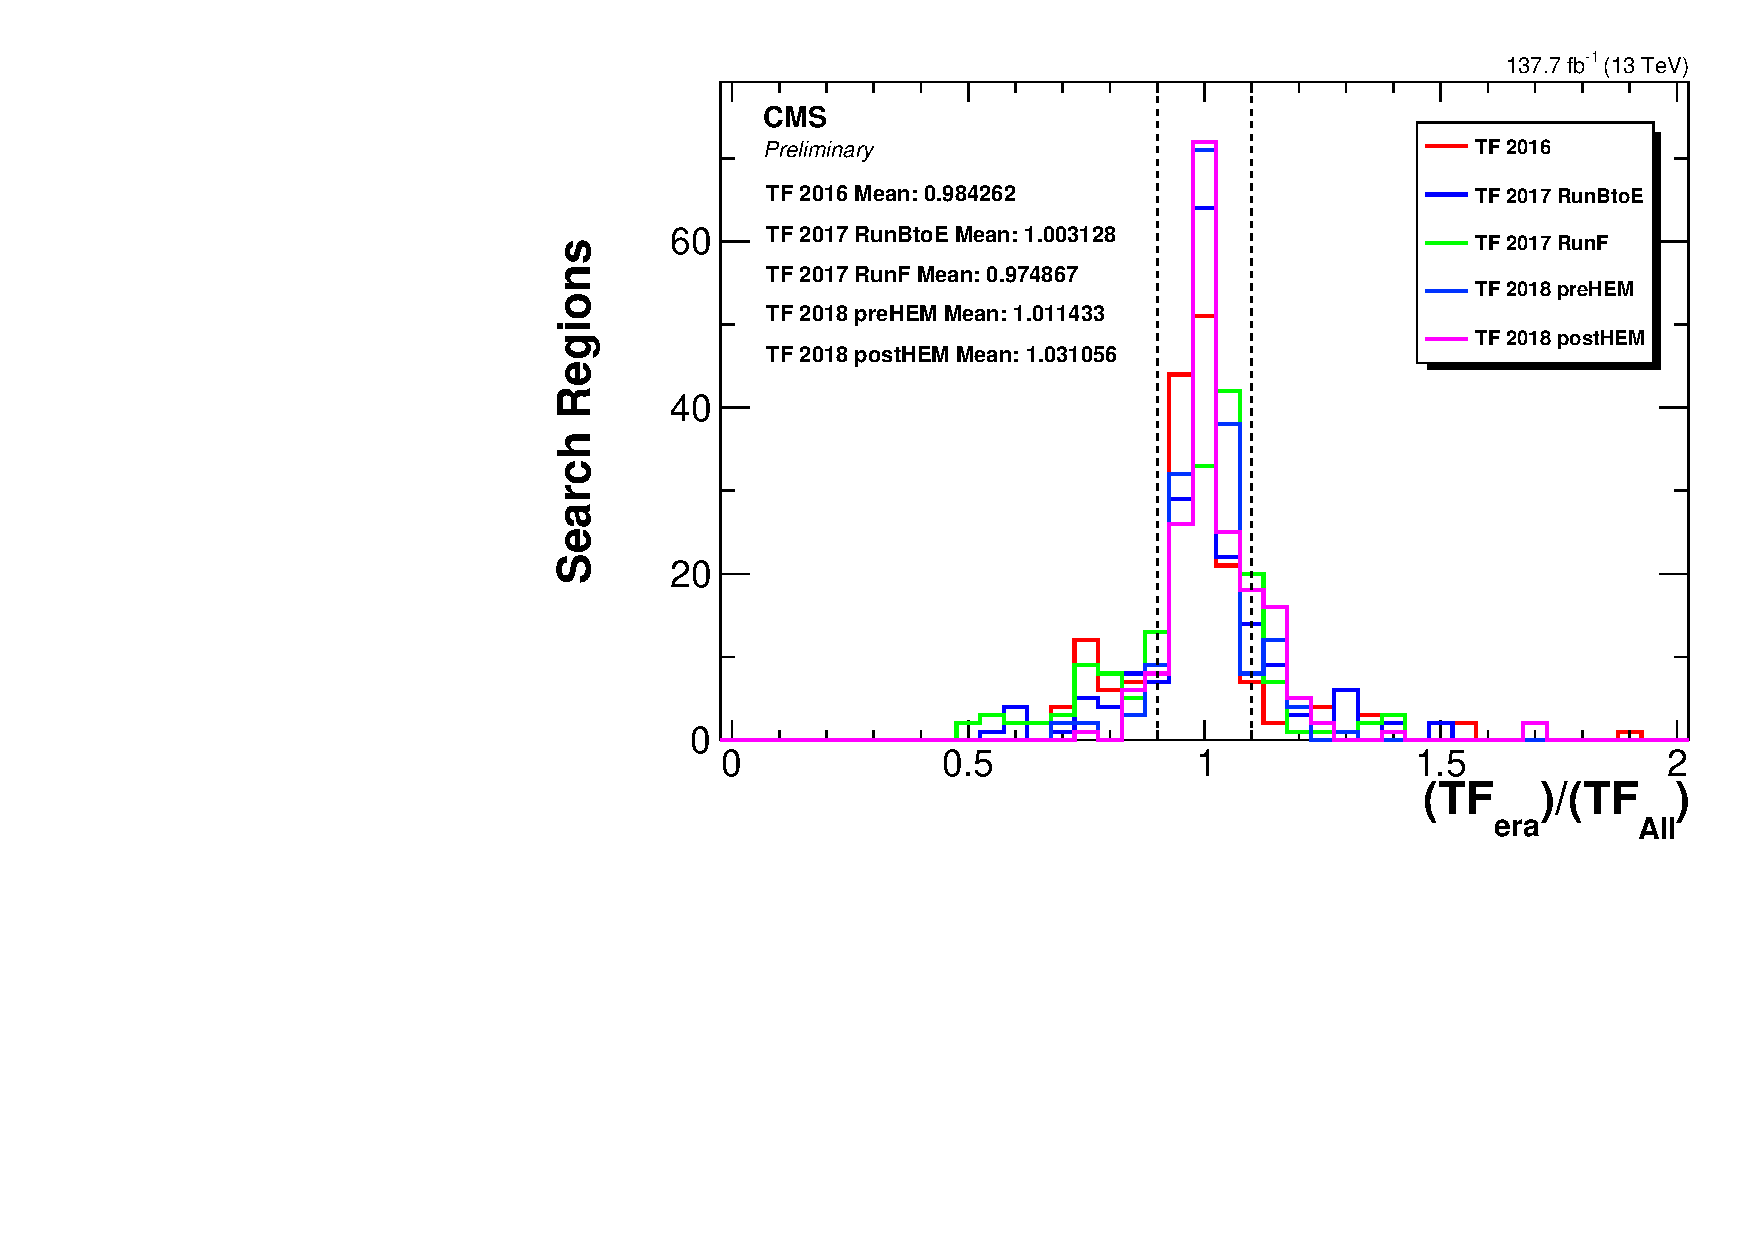
\includegraphics[width=0.5\textwidth]{LostLepton_TF_CR_to_SR_noextrap_Comparison_sum.pdf} \\
		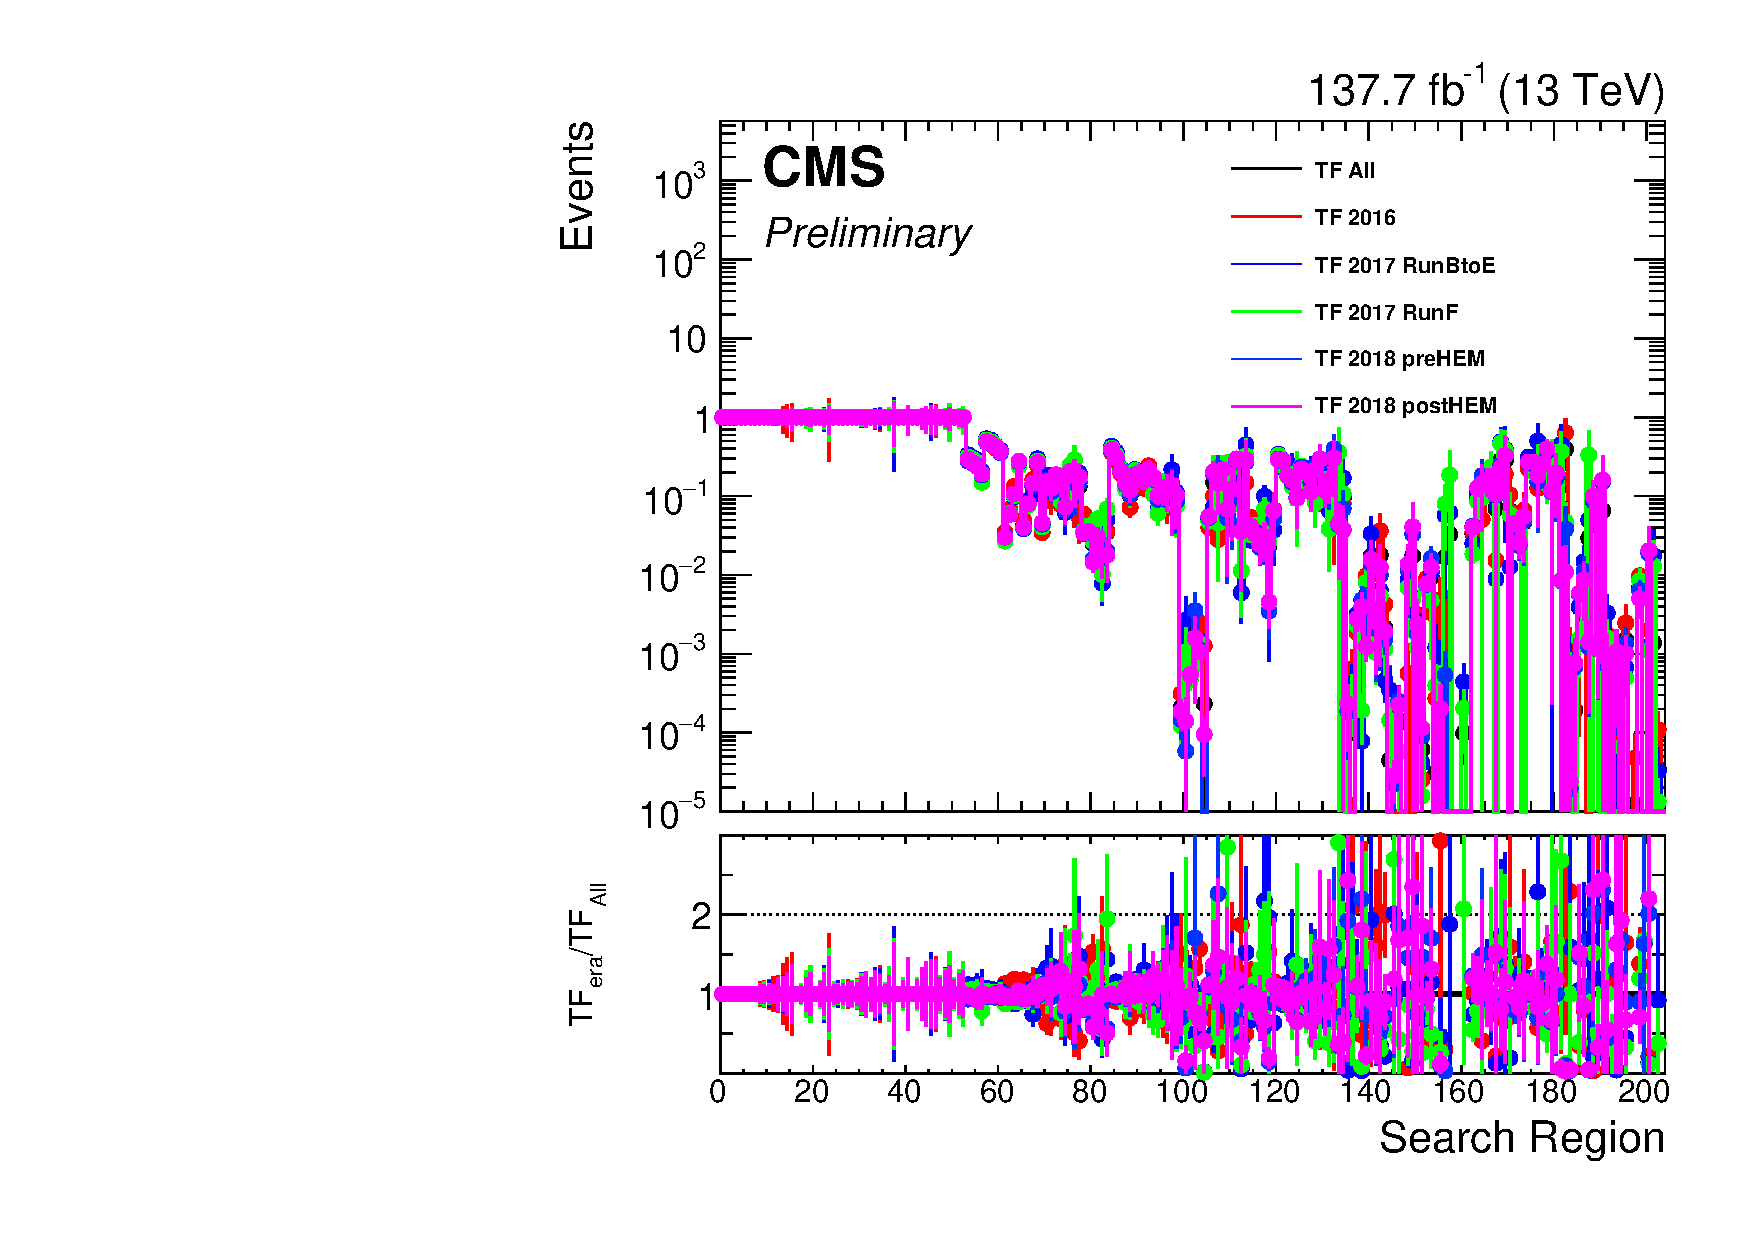
\includegraphics[width=0.4\textwidth]{LostLepton_TF_SR_extrap_Comparison.pdf}
		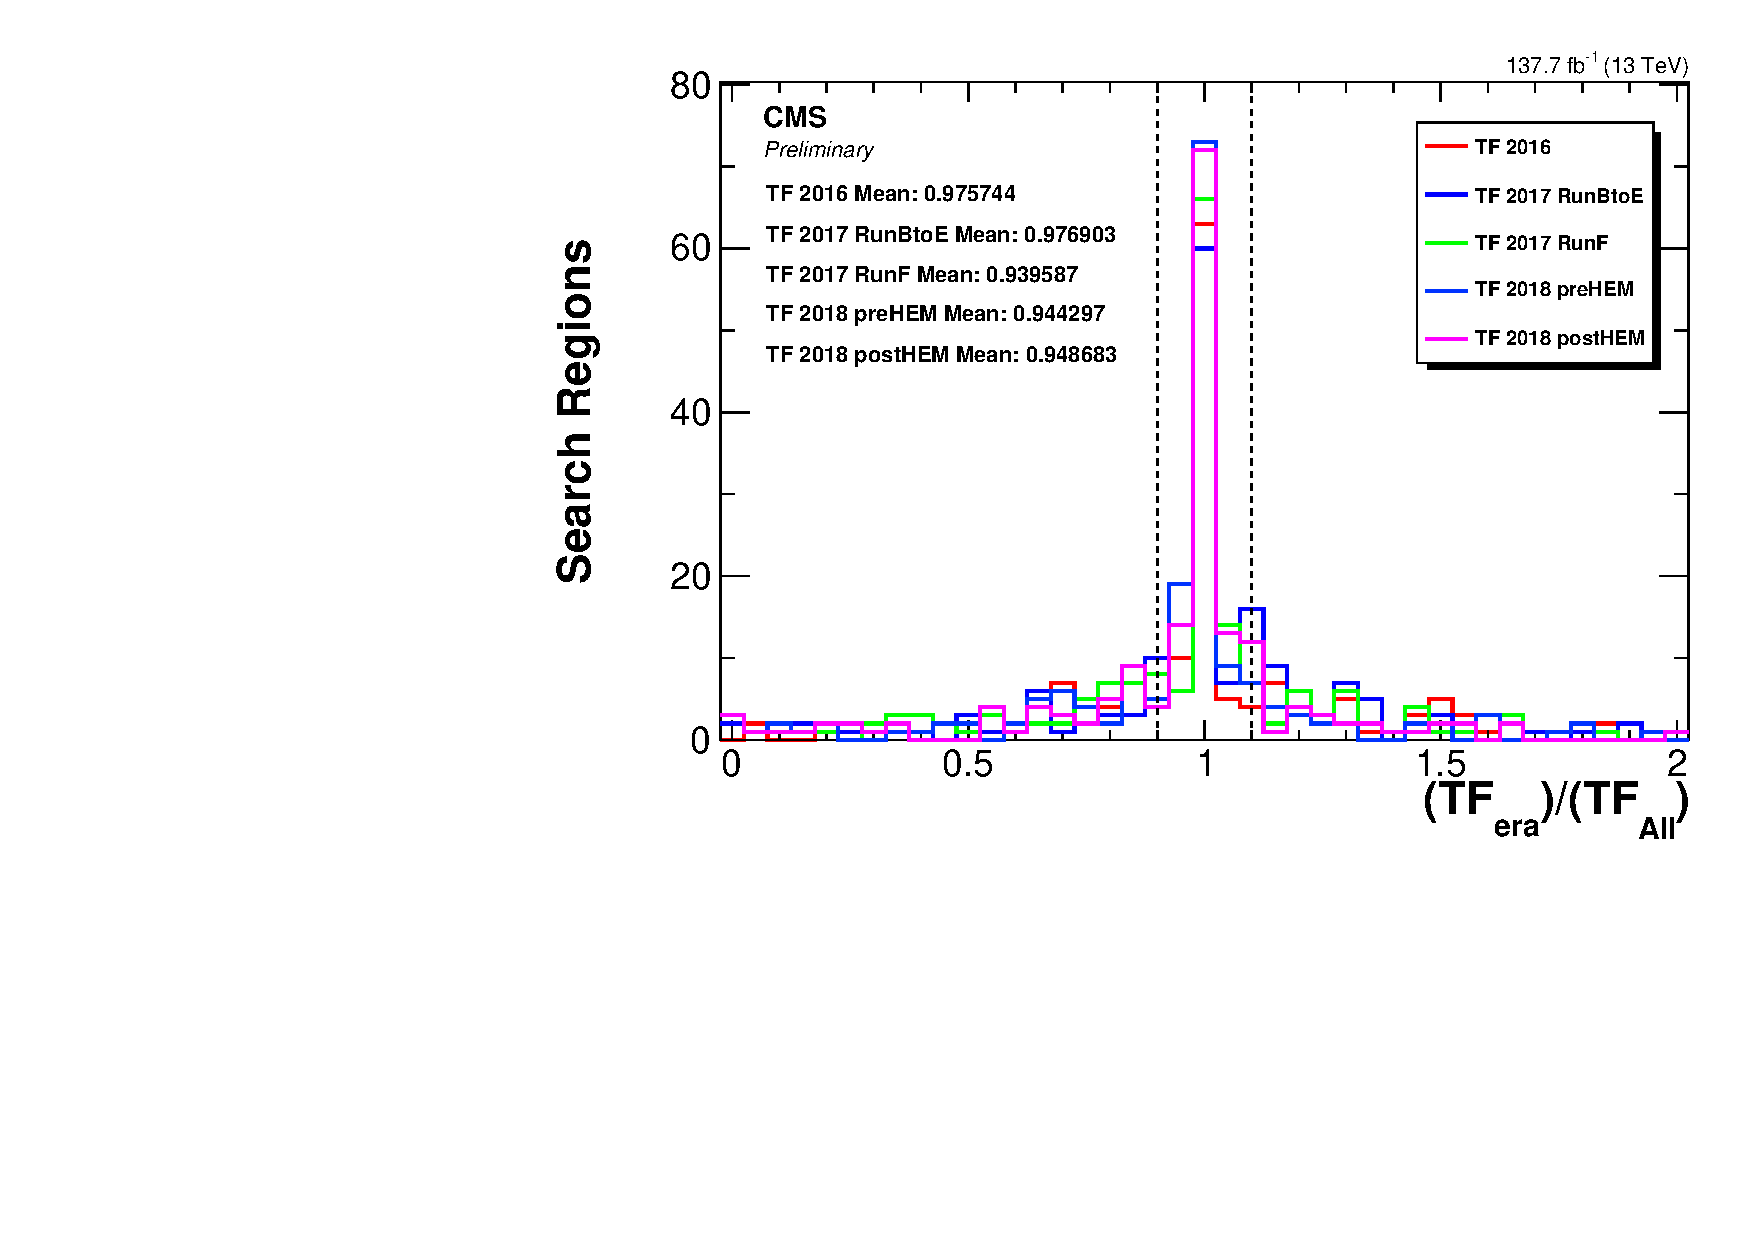
\includegraphics[width=0.5\textwidth]{LostLepton_TF_SR_extrap_Comparison_sum.pdf}
	\end{center}
	\caption[Separated Transfer Factor Comparison]{Comparisons of the transfer factors, separated into the CR-to-SR (top) and SR-to-extrapolation (bottom), for each era of MC in the low and high \dm{} regions. The values are shown in their separate bins on the left plot and in a combined form on the right. The mean for each is also shown. 
	 }
	\label{fig:llb-1lcr-datavsmc-sep-tf}
\end{figure}

% matches pred table
% copy and paste the output from the end of LLBPred() (it calls printMoriond17Table) between the below labels "start insert" and "stop insert".
\begin{table}[!!htbp]
\begin{center}
\resizebox*{0.6\textwidth}{!}{
\begin{tabular}{|c||c||c|c|c|}
\hline
Search Region & \met [GeV] & $N_{\text{data}}(1l)$ & $\tfll$ & $N_\text{pred}^{\text{LL}}$ \\
\hline
% Search region & 	$\met$ & 	singlelep & 	_TF & 	_pred & 	
\hline
\multicolumn{5}{c}{low \dm, $\nb=0$, $\nsv=0$, $\ptisr\geq500$\,GeV, $2\leq\nj\leq5$} \\
\hline
 %  lm_nb0_nivf0_highptisr_nj2to5
0 & 450$-$550 & 	5045 & 	0.432$\pm$0.004 & 	2178.23$\pm$35.68 \\
1 & 550$-$650 & 	2198 & 	0.509$\pm$0.004 & 	1118.77$\pm$25.67 \\
2 & 650$-$750 & 	818 & 	0.516$\pm$0.004 & 	421.97$\pm$15.16 \\
3 & $\geq750$ & 	540 & 	0.509$\pm$0.004 & 	274.59$\pm$12.04 \\
\hline
\multicolumn{5}{c}{low \dm, $\nb=0$, $\nsv=0$, $\ptisr\geq500$\,GeV, $\nj\geq6$} \\
\hline
 %     lm_nb0_nivf0_highptisr_nj6
4 & 450$-$550 & 	849 & 	0.333$\pm$0.004 & 	282.81$\pm$10.32 \\
5 & 550$-$650 & 	408 & 	0.338$\pm$0.005 & 	137.77$\pm$7.14 \\
6 & 650$-$750 & 	181 & 	0.331$\pm$0.006 & 	59.90$\pm$4.60 \\
7 & $\geq750$ & 	156 & 	0.321$\pm$0.006 & 	50.12$\pm$4.11 \\
\hline
\multicolumn{5}{c}{low \dm, $\nb=0$, $\nsv\geq1$, $\ptisr\geq500$\,GeV, $2\leq\nj\leq5$} \\
\hline
 %  lm_nb0_nivf1_highptisr_nj2to5
8 & 450$-$550 & 	148 & 	0.537$\pm$0.024 & 	79.42$\pm$7.44 \\
9 & 550$-$650 & 	38 & 	0.581$\pm$0.026 & 	22.09$\pm$3.71 \\
10 & 650$-$750 & 	25 & 	0.641$\pm$0.032 & 	16.03$\pm$3.31 \\
11 & $\geq750$ & 	16 & 	0.609$\pm$0.027 & 	9.75$\pm$2.48 \\
\hline
\multicolumn{5}{c}{low \dm, $\nb=0$, $\nsv\geq1$, $\ptisr\geq500$\,GeV, $\nj\geq6$} \\
\hline
 %     lm_nb0_nivf1_highptisr_nj6
12 & 450$-$550 & 	43 & 	0.410$\pm$0.028 & 	17.64$\pm$2.96 \\
13 & 550$-$650 & 	12 & 	0.415$\pm$0.037 & 	4.98$\pm$1.50 \\
14 & 650$-$750 & 	5 & 	0.414$\pm$0.040 & 	2.07$\pm$0.95 \\
15 & $\geq750$ & 	4 & 	0.341$\pm$0.041 & 	1.36$\pm$0.70 \\
\hline
\multicolumn{5}{c}{low \dm, $\nb=1$, $\nsv=0$, $\mtb<175$~\GeV, $300\leq\ptisr<500$\,GeV, $\ptb<40$\,GeV} \\
\hline
 % lm_nb1_nivf0_lowmtb_lowptisr_lowptb
16 & 300$-$400 & 	2037 & 	0.746$\pm$0.015 & 	1520.34$\pm$45.84 \\
17 & 400$-$500 & 	341 & 	0.724$\pm$0.031 & 	246.78$\pm$16.96 \\
18 & 500$-$600 & 	32 & 	0.726$\pm$0.061 & 	23.24$\pm$4.55 \\
19 & $\geq600$ & 	6 & 	0.581$\pm$0.068 & 	3.48$\pm$1.48 \\
\hline
\multicolumn{5}{c}{low \dm, $\nb=1$, $\nsv=0$, $\mtb<175$~\GeV, $300\leq\ptisr<500$\,GeV, $40<\ptb<70$\,GeV} \\
\hline
 % lm_nb1_nivf0_lowmtb_lowptisr_medptb
20 & 300$-$400 & 	1015 & 	0.716$\pm$0.019 & 	726.30$\pm$29.71 \\
21 & 400$-$500 & 	127 & 	0.786$\pm$0.047 & 	99.84$\pm$10.68 \\
22 & 500$-$600 & 	11 & 	0.655$\pm$0.076 & 	7.21$\pm$2.33 \\
23 & $\geq600$ & 	6 & 	0.524$\pm$0.115 & 	3.15$\pm$1.46 \\
\hline
\multicolumn{5}{c}{low \dm, $\nb=1$, $\nsv=0$, $\mtb<175$~\GeV, $\ptisr\geq500$\,GeV, $\ptb<40$\,GeV} \\
\hline
 % lm_nb1_nivf0_lowmtb_highptisr_lowptb
24 & 450$-$550 & 	136 & 	0.579$\pm$0.027 & 	78.76$\pm$7.72 \\
25 & 550$-$650 & 	45 & 	0.686$\pm$0.034 & 	30.87$\pm$4.85 \\
26 & 650$-$750 & 	12 & 	0.537$\pm$0.033 & 	6.44$\pm$1.90 \\
27 & $\geq750$ & 	14 & 	0.576$\pm$0.034 & 	8.07$\pm$2.21 \\
\hline
\multicolumn{5}{c}{low \dm, $\nb=1$, $\nsv=0$, $\mtb<175$~\GeV, $\ptisr\geq500$\,GeV, $40<\ptb<70$\,GeV} \\
\hline
 % lm_nb1_nivf0_lowmtb_highptisr_medptb
28 & 450$-$550 & 	89 & 	0.676$\pm$0.039 & 	60.14$\pm$7.25 \\
29 & 550$-$650 & 	19 & 	0.722$\pm$0.045 & 	13.72$\pm$3.26 \\
30 & 650$-$750 & 	11 & 	0.589$\pm$0.053 & 	6.47$\pm$2.04 \\
31 & $\geq750$ & 	3 & 	0.654$\pm$0.066 & 	1.96$\pm$1.15 \\
\hline
\multicolumn{5}{c}{low \dm, $\nb=1$, $\nsv\geq1$, $\mtb<175$~\GeV, $\ptb<40$\,GeV} \\
\hline
 %     lm_nb1_nivf1_lowmtb_lowptb
32 & 300$-$400 & 	115 & 	0.741$\pm$0.054 & 	85.23$\pm$10.10 \\
33 & 400$-$500 & 	26 & 	0.587$\pm$0.069 & 	15.26$\pm$3.49 \\
34 & $\geq500$ & 	13 & 	0.640$\pm$0.071 & 	8.32$\pm$2.49 \\
\hline
\multicolumn{5}{c}{low \dm, $\nb\geq2$, $\mtb<175$~\GeV, $300\leq\ptisr<500$\,GeV, $\ptbonetwo<80$\,GeV} \\
\hline
 % lm_nb2_lowmtb_lowptisr_lowptb12
35 & 300$-$400 & 	242 & 	0.603$\pm$0.028 & 	145.92$\pm$11.59 \\
36 & 400$-$500 & 	36 & 	0.667$\pm$0.066 & 	24.00$\pm$4.65 \\
37 & $\geq500$ & 	7 & 	0.704$\pm$0.169 & 	4.93$\pm$2.21 \\
\hline
\multicolumn{5}{c}{low \dm, $\nb\geq2$, $\mtb<175$~\GeV, $300\leq\ptisr<500$\,GeV, $80<\ptbonetwo<140$\,GeV} \\
\hline
 % lm_nb2_lowmtb_lowptisr_medptb12
38 & 300$-$400 & 	579 & 	0.554$\pm$0.015 & 	320.86$\pm$15.79 \\
39 & 400$-$500 & 	101 & 	0.694$\pm$0.045 & 	70.12$\pm$8.31 \\
40 & $\geq500$ & 	16 & 	0.525$\pm$0.081 & 	8.40$\pm$2.47 \\
\hline
\multicolumn{5}{c}{low \dm, $\nb\geq2$, $\mtb<175$~\GeV, $300\leq\ptisr<500$\,GeV, $\ptbonetwo\geq140$\,GeV, $\nj\geq7$} \\
\hline
 % lm_nb2_lowmtb_lowptisr_highptb12_nj7
41 & 300$-$400 & 	318 & 	0.516$\pm$0.016 & 	164.19$\pm$10.49 \\
42 & 400$-$500 & 	53 & 	0.494$\pm$0.031 & 	26.19$\pm$3.96 \\
43 & $\geq500$ & 	9 & 	0.706$\pm$0.088 & 	6.36$\pm$2.26 \\
\hline
\multicolumn{5}{c}{low \dm, $\nb\geq2$, $\mtb<175$~\GeV, $\ptisr\geq500$\,GeV, $\ptbonetwo<80$\,GeV} \\
\hline
 % lm_nb2_lowmtb_highptisr_lowptb12
44 & 450$-$550 & 	19 & 	0.356$\pm$0.047 & 	6.77$\pm$1.79 \\
45 & 550$-$650 & 	7 & 	0.469$\pm$0.075 & 	3.29$\pm$1.35 \\
46 & $\geq650$ & 	2 & 	0.366$\pm$0.057 & 	0.73$\pm$0.53 \\
\hline
\multicolumn{5}{c}{low \dm, $\nb\geq2$, $\mtb<175$~\GeV, $\ptisr\geq500$\,GeV, $80<\ptbonetwo<140$\,GeV} \\
\hline
 % lm_nb2_lowmtb_highptisr_medptb12
47 & 450$-$550 & 	50 & 	0.447$\pm$0.035 & 	22.33$\pm$3.60 \\
48 & 550$-$650 & 	16 & 	0.631$\pm$0.074 & 	10.10$\pm$2.79 \\
49 & $\geq650$ & 	6 & 	0.699$\pm$0.103 & 	4.20$\pm$1.82 \\
\hline
\multicolumn{5}{c}{low \dm, $\nb\geq2$, $\mtb<175$~\GeV, $\ptisr\geq500$\,GeV, $\ptbonetwo\geq140$\,GeV, $\nj\geq7$} \\
\hline
 % lm_nb2_lowmtb_highptisr_highptb12_nj7
50 & 450$-$550 & 	59 & 	0.429$\pm$0.027 & 	25.31$\pm$3.67 \\
51 & 550$-$650 & 	19 & 	0.649$\pm$0.063 & 	12.32$\pm$3.07 \\
52 & $\geq650$ & 	7 & 	0.559$\pm$0.070 & 	3.91$\pm$1.56 \\
\hline
\end{tabular}
}
\caption{\label{tab:0l-llb-pred-lm}The LL estimate in the various low \dm{} search regions, bins 0 to 53, using the \datalumi~dataset.}
\end{center}
\end{table}
% matches pred table
% copy and paste the output from the end of LLBPred() (it calls printMoriond17Table) between the below labels "start insert" and "stop insert".
\begin{table}[!h]
\begin{center}
\resizebox*{0.6\textwidth}{!}{
\begin{tabular}{|c||c||c|c|c|c|c|}
\hline
Search Region & \met [GeV] & $N_{\text{data}}(1l)$ & $\tfll$ & $\tfll^{\text{CR-SR}}$ & $\tfll^{\text{SR-extrap}}$ & $N_\text{pred}^{\text{LL}}$ \\
\hline
% Search region & 	$\met$ & 	singlelep & 	_TF & 	_TF_CR_to_SR_noextrap & 	_TF_SR_extrap & 	_pred & 	
\hline
\multicolumn{7}{c}{high \dm, $\nb=1$, $\mtb<175$~\GeV, $\nj\geq7$, $\nrt\geq1$} \\
\hline
 %      hm_nb1_lowmtb_nj7_nrtgeq1
53 & 250$-$300 & 	1151 & 	0.196$\pm$0.004 & 	0.519 & 	0.378 & 	225.43$\pm$8.24 \\
54 & 300$-$400 & 	697 & 	0.187$\pm$0.005 & 	0.550 & 	0.340 & 	130.35$\pm$6.21 \\
55 & 400$-$500 & 	129 & 	0.180$\pm$0.011 & 	0.577 & 	0.313 & 	23.26$\pm$2.53 \\
56 & $\geq500$ & 	43 & 	0.157$\pm$0.016 & 	0.598 & 	0.263 & 	6.77$\pm$1.25 \\
\hline
\multicolumn{7}{c}{high \dm, $\nb\geq2$, $\mtb<175$~\GeV, $\nj\geq7$, $\nrt\geq1$} \\
\hline
 %      hm_nb2_lowmtb_nj7_nrtgeq1
57 & 250$-$300 & 	2250 & 	0.292$\pm$0.004 & 	0.539 & 	0.542 & 	657.73$\pm$16.12 \\
58 & 300$-$400 & 	1256 & 	0.286$\pm$0.005 & 	0.548 & 	0.522 & 	359.11$\pm$11.69 \\
59 & 400$-$500 & 	236 & 	0.278$\pm$0.010 & 	0.582 & 	0.478 & 	65.56$\pm$4.92 \\
60 & $\geq500$ & 	99 & 	0.259$\pm$0.017 & 	0.625 & 	0.415 & 	25.67$\pm$3.06 \\
\hline
\multicolumn{7}{c}{high \dm, $\nb=1$, $\mtb\geq175$~\GeV, $\nt=0$, $\nrt=0$, $\nw=0$, $\Ht\geq1000$} \\
\hline
 % hm_nb1_highmtb_nt0_nrt0_nw0_htgt1000
61 & 250$-$350 & 	570 & 	0.383$\pm$0.007 & 	0.657 & 	0.583 & 	218.28$\pm$10.01 \\
62 & 350$-$450 & 	233 & 	0.369$\pm$0.011 & 	0.614 & 	0.602 & 	86.03$\pm$6.16 \\
63 & 450$-$550 & 	102 & 	0.362$\pm$0.015 & 	0.544 & 	0.666 & 	36.97$\pm$3.96 \\
64 & $\geq550$ & 	109 & 	0.352$\pm$0.013 & 	0.531 & 	0.663 & 	38.39$\pm$3.93 \\
\hline
\multicolumn{7}{c}{high \dm, $\nb\geq2$, $\mtb\geq175$~\GeV, $\nt=0$, $\nrt=0$, $\nw=0$, $\Ht\geq1000$} \\
\hline
 % hm_nb2_highmtb_nt0_nrt0_nw0_htgt1000
65 & 250$-$350 & 	186 & 	0.359$\pm$0.013 & 	0.738 & 	0.486 & 	66.78$\pm$5.49 \\
66 & 350$-$450 & 	57 & 	0.379$\pm$0.021 & 	0.675 & 	0.561 & 	21.58$\pm$3.11 \\
67 & 450$-$550 & 	23 & 	0.334$\pm$0.027 & 	0.616 & 	0.542 & 	7.69$\pm$1.72 \\
68 & $\geq550$ & 	32 & 	0.317$\pm$0.025 & 	0.537 & 	0.590 & 	10.14$\pm$1.97 \\
\hline
\multicolumn{7}{c}{high \dm, $\nb=1$, $\mtb\geq175$~\GeV, $\nt\geq1$, $\nrt=0$, $\nw=0$, $\Ht<1000$} \\
\hline
 % hm_nb1_highmtb_ntgeq1_nrt0_nw0_htlt1000
69 & 250$-$550 & 	11329 & 	0.035$\pm$0.001 & 	0.601 & 	0.058 & 	397.77$\pm$7.71 \\
70 & 550$-$650 & 	87 & 	0.081$\pm$0.010 & 	0.553 & 	0.147 & 	7.07$\pm$1.14 \\
71 & $\geq650$ & 	29 & 	0.075$\pm$0.015 & 	0.684 & 	0.110 & 	2.18$\pm$0.59 \\
\hline
\multicolumn{7}{c}{high \dm, $\nb=1$, $\mtb\geq175$~\GeV, $\nt\geq1$, $\nrt=0$, $\nw=0$, $1000\leq\Ht<1500$} \\
\hline
 % hm_nb1_highmtb_ntgeq1_nrt0_nw0_ht1000to1500
72 & 250$-$550 & 	739 & 	0.111$\pm$0.004 & 	0.621 & 	0.179 & 	81.90$\pm$4.07 \\
73 & 550$-$650 & 	36 & 	0.063$\pm$0.011 & 	0.507 & 	0.125 & 	2.27$\pm$0.55 \\
74 & $\geq650$ & 	42 & 	0.053$\pm$0.011 & 	0.539 & 	0.098 & 	2.23$\pm$0.56 \\
\hline
\multicolumn{7}{c}{high \dm, $\nb=1$, $\mtb\geq175$~\GeV, $\nt\geq1$, $\nrt=0$, $\nw=0$, $\Ht\geq1500$} \\
\hline
 % hm_nb1_highmtb_ntgeq1_nrt0_nw0_htgt1500
75 & 250$-$550 & 	166 & 	0.131$\pm$0.008 & 	0.690 & 	0.190 & 	21.70$\pm$2.19 \\
76 & 550$-$650 & 	8 & 	0.124$\pm$0.030 & 	0.637 & 	0.195 & 	0.99$\pm$0.43 \\
77 & $\geq650$ & 	23 & 	0.079$\pm$0.019 & 	0.506 & 	0.156 & 	1.81$\pm$0.57 \\
\hline
\multicolumn{7}{c}{high \dm, $\nb=1$, $\mtb\geq175$~\GeV, $\nt=0$, $\nrt=0$, $\nw\geq1$, $\Ht<1300$} \\
\hline
 % hm_nb1_highmtb_nt0_nrt0_nwgeq1_htlt1300
78 & 250$-$350 & 	9720 & 	0.023$\pm$0.000 & 	0.594 & 	0.038 & 	220.56$\pm$5.06 \\
79 & 350$-$450 & 	1773 & 	0.023$\pm$0.001 & 	0.638 & 	0.036 & 	40.40$\pm$2.18 \\
80 & $\geq450$ & 	586 & 	0.015$\pm$0.001 & 	0.612 & 	0.025 & 	9.07$\pm$0.94 \\
\hline
\multicolumn{7}{c}{high \dm, $\nb=1$, $\mtb\geq175$~\GeV, $\nt=0$, $\nrt=0$, $\nw\geq1$, $\Ht\geq1300$} \\
\hline
 % hm_nb1_highmtb_nt0_nrt0_nwgeq1_htgt1300
81 & 250$-$350 & 	206 & 	0.023$\pm$0.003 & 	0.718 & 	0.032 & 	4.67$\pm$0.68 \\
82 & 350$-$450 & 	87 & 	0.011$\pm$0.002 & 	0.607 & 	0.018 & 	0.94$\pm$0.22 \\
83 & $\geq450$ & 	87 & 	0.021$\pm$0.004 & 	0.545 & 	0.038 & 	1.82$\pm$0.37 \\
\hline
\multicolumn{7}{c}{high \dm, $\nb=1$, $\mtb\geq175$~\GeV, $\nt=0$, $\nrt\geq1$, $\nw=0$, $\Ht<1000$} \\
\hline
 % hm_nb1_highmtb_nt0_nrtgeq1_nw0_htlt1000
84 & 250$-$350 & 	9356 & 	0.253$\pm$0.002 & 	0.592 & 	0.427 & 	2362.92$\pm$30.67 \\
85 & 350$-$450 & 	1627 & 	0.227$\pm$0.004 & 	0.640 & 	0.355 & 	369.27$\pm$11.50 \\
86 & 450$-$550 & 	346 & 	0.169$\pm$0.007 & 	0.652 & 	0.259 & 	58.49$\pm$4.01 \\
87 & 550$-$650 & 	87 & 	0.123$\pm$0.011 & 	0.553 & 	0.223 & 	10.73$\pm$1.49 \\
88 & $\geq650$ & 	29 & 	0.118$\pm$0.017 & 	0.684 & 	0.173 & 	3.44$\pm$0.80 \\
\hline
\multicolumn{7}{c}{high \dm, $\nb=1$, $\mtb\geq175$~\GeV, $\nt=0$, $\nrt\geq1$, $\nw=0$, $1000\leq\Ht<1500$} \\
\hline
 % hm_nb1_highmtb_nt0_nrtgeq1_nw0_ht1000to1500
89 & 250$-$350 & 	470 & 	0.126$\pm$0.005 & 	0.639 & 	0.198 & 	59.43$\pm$3.64 \\
90 & 350$-$450 & 	187 & 	0.128$\pm$0.008 & 	0.619 & 	0.207 & 	23.93$\pm$2.35 \\
91 & 450$-$550 & 	82 & 	0.089$\pm$0.009 & 	0.520 & 	0.171 & 	7.28$\pm$1.11 \\
92 & 550$-$650 & 	36 & 	0.121$\pm$0.016 & 	0.507 & 	0.239 & 	4.36$\pm$0.93 \\
93 & $\geq650$ & 	42 & 	0.086$\pm$0.011 & 	0.539 & 	0.160 & 	3.61$\pm$0.73 \\
\hline
\end{tabular}
}
\caption[LL HM CR bins 53-93]{\label{tab:0l-llb-pred-hm-1}The LL estimate in the various high \dm{} search regions, bins 53 to 93, using the \datalumi~dataset.}
\end{center}
\end{table}
% matches pred table
% copy and paste the output from the end of LLBPred() (it calls printMoriond17Table) between the below labels "start insert" and "stop insert".
\begin{table}[!h]
\begin{center}
\resizebox*{0.6\textwidth}{!}{
\begin{tabular}{|c||c||c|c|c|c|c|}
\hline
Search Region & \met [GeV] & $N_{\text{data}}(1l)$ & $\tfll$ & $\tfll^{\text{CR-SR}}$ & $\tfll^{\text{SR-extrap}}$ & $N_\text{pred}^{\text{LL}}$ \\
\hline
\multicolumn{7}{c}{high \dm, $\nb=1$, $\mtb\geq175$~\GeV, $\nt=0$, $\nrt\geq1$, $\nw=0$, $\Ht\geq1500$} \\
\hline
 % hm_nb1_highmtb_nt0_nrtgeq1_nw0_htgt1500
94 & 250$-$350 & 	100 & 	0.075$\pm$0.008 & 	0.744 & 	0.100 & 	7.46$\pm$1.06 \\
95 & 350$-$450 & 	46 & 	0.069$\pm$0.011 & 	0.589 & 	0.118 & 	3.19$\pm$0.68 \\
96 & 450$-$550 & 	20 & 	0.087$\pm$0.017 & 	0.649 & 	0.135 & 	1.75$\pm$0.52 \\
97 & 550$-$650 & 	8 & 	0.101$\pm$0.029 & 	0.637 & 	0.158 & 	0.80$\pm$0.37 \\
98 & $\geq650$ & 	23 & 	0.040$\pm$0.011 & 	0.506 & 	0.079 & 	0.92$\pm$0.31 \\
\hline
\multicolumn{7}{c}{high \dm, $\nb=1$, $\mtb\geq175$~\GeV, $\nt\geq1$, $\nrt=0$, $\nw\geq1$} \\
\hline
 % hm_nb1_highmtb_ntgeq1_nrt0_nwgeq1
99 & 250$-$550 & 	12234 & 	0.000$\pm$0.000 & 	0.604 & 	0.000 & 	2.42$\pm$0.44 \\
100 & $\geq550$ & 	225 & 	0.001$\pm$0.000 & 	0.557 & 	0.001 & 	0.16$\pm$0.10 \\
\hline
\multicolumn{7}{c}{high \dm, $\nb=1$, $\mtb\geq175$~\GeV, $\nt\geq1$, $\nrt\geq1$, $\nw=0$} \\
\hline
 % hm_nb1_highmtb_ntgeq1_nrtgeq1_nw0
101 & 250$-$550 & 	12234 & 	0.001$\pm$0.000 & 	0.604 & 	0.001 & 	6.76$\pm$0.80 \\
102 & $\geq550$ & 	225 & 	0.002$\pm$0.001 & 	0.557 & 	0.003 & 	0.35$\pm$0.13 \\
\hline
\multicolumn{7}{c}{high \dm, $\nb=1$, $\mtb\geq175$~\GeV, $\nt=0$, $\nrt\geq1$, $\nw\geq1$} \\
\hline
 % hm_nb1_highmtb_nt0_nrtgeq1_nwgeq1
103 & 250$-$550 & 	12234 & 	0.001$\pm$0.000 & 	0.604 & 	0.002 & 	17.29$\pm$1.17 \\
104 & $\geq550$ & 	225 & 	0.000$\pm$0.000 & 	0.557 & 	0.001 & 	0.08$\pm$0.07 \\
\hline
\multicolumn{7}{c}{high \dm, $\nb=2$, $\mtb\geq175$~\GeV, $\nt=1$, $\nrt=0$, $\nw=0$, $\Ht<1000$} \\
\hline
 % hm_nbeq2_highmtb_nt1_nrt0_nw0_htlt1000
105 & 250$-$550 & 	2055 & 	0.040$\pm$0.001 & 	0.650 & 	0.062 & 	82.37$\pm$3.55 \\
106 & 550$-$650 & 	15 & 	0.108$\pm$0.022 & 	0.614 & 	0.176 & 	1.62$\pm$0.53 \\
107 & $\geq650$ & 	7 & 	0.084$\pm$0.030 & 	0.737 & 	0.115 & 	0.59$\pm$0.31 \\
\hline
\multicolumn{7}{c}{high \dm, $\nb=2$, $\mtb\geq175$~\GeV, $\nt=1$, $\nrt=0$, $\nw=0$, $1000\leq\Ht<1500$} \\
\hline
 % hm_nbeq2_highmtb_nt1_nrt0_nw0_ht1000to1500
108 & 250$-$550 & 	151 & 	0.149$\pm$0.009 & 	0.710 & 	0.210 & 	22.56$\pm$2.25 \\
109 & 550$-$650 & 	7 & 	0.042$\pm$0.016 & 	0.521 & 	0.080 & 	0.29$\pm$0.15 \\
110 & $\geq650$ & 	13 & 	0.089$\pm$0.028 & 	0.539 & 	0.165 & 	1.16$\pm$0.48 \\
\hline
\multicolumn{7}{c}{high \dm, $\nb=2$, $\mtb\geq175$~\GeV, $\nt=1$, $\nrt=0$, $\nw=0$, $\Ht\geq1500$} \\
\hline
 % hm_nbeq2_highmtb_nt1_nrt0_nw0_htgt1500
111 & 250$-$550 & 	45 & 	0.202$\pm$0.022 & 	0.819 & 	0.246 & 	9.07$\pm$1.67 \\
112 & 550$-$650 & 	3 & 	0.052$\pm$0.035 & 	0.418 & 	0.126 & 	0.16$\pm$0.14 \\
113 & $\geq650$ & 	5 & 	0.134$\pm$0.044 & 	0.446 & 	0.301 & 	0.67$\pm$0.37 \\
\hline
\multicolumn{7}{c}{high \dm, $\nb=2$, $\mtb\geq175$~\GeV, $\nt=0$, $\nrt=0$, $\nw=1$, $\Ht<1300$} \\
\hline
 % hm_nbeq2_highmtb_nt0_nrt0_nw1_htlt1300
114 & 250$-$350 & 	1742 & 	0.025$\pm$0.001 & 	0.657 & 	0.038 & 	43.11$\pm$2.60 \\
115 & 350$-$450 & 	340 & 	0.023$\pm$0.002 & 	0.656 & 	0.036 & 	7.96$\pm$0.92 \\
116 & $\geq450$ & 	121 & 	0.014$\pm$0.003 & 	0.601 & 	0.023 & 	1.71$\pm$0.40 \\
\hline
\multicolumn{7}{c}{high \dm, $\nb=2$, $\mtb\geq175$~\GeV, $\nt=0$, $\nrt=0$, $\nw=1$, $\Ht\geq1300$} \\
\hline
 % hm_nbeq2_highmtb_nt0_nrt0_nw1_htgt1300
117 & 250$-$350 & 	52 & 	0.028$\pm$0.006 & 	0.793 & 	0.036 & 	1.47$\pm$0.38 \\
118 & 350$-$450 & 	21 & 	0.017$\pm$0.008 & 	0.828 & 	0.021 & 	0.36$\pm$0.19 \\
119 & $\geq450$ & 	25 & 	0.035$\pm$0.011 & 	0.566 & 	0.062 & 	0.87$\pm$0.33 \\
\hline
\multicolumn{7}{c}{high \dm, $\nb=2$, $\mtb\geq175$~\GeV, $\nt=0$, $\nrt=1$, $\nw=0$, $\Ht<1000$} \\
\hline
 % hm_nbeq2_highmtb_nt0_nrt1_nw0_htlt1000
120 & 250$-$350 & 	1661 & 	0.225$\pm$0.004 & 	0.651 & 	0.346 & 	373.86$\pm$11.68 \\
121 & 350$-$450 & 	317 & 	0.196$\pm$0.009 & 	0.659 & 	0.297 & 	62.06$\pm$4.44 \\
122 & 450$-$550 & 	77 & 	0.147$\pm$0.014 & 	0.605 & 	0.243 & 	11.32$\pm$1.69 \\
123 & 550$-$650 & 	15 & 	0.143$\pm$0.026 & 	0.614 & 	0.234 & 	2.15$\pm$0.68 \\
124 & $\geq650$ & 	7 & 	0.173$\pm$0.048 & 	0.737 & 	0.235 & 	1.21$\pm$0.57 \\
\hline
\multicolumn{7}{c}{high \dm, $\nb=2$, $\mtb\geq175$~\GeV, $\nt=0$, $\nrt=1$, $\nw=0$, $1000\leq\Ht<1500$} \\
\hline
 % hm_nbeq2_highmtb_nt0_nrt1_nw0_ht1000to1500
125 & 250$-$350 & 	105 & 	0.171$\pm$0.011 & 	0.752 & 	0.227 & 	17.91$\pm$2.12 \\
126 & 350$-$450 & 	30 & 	0.119$\pm$0.014 & 	0.663 & 	0.180 & 	3.57$\pm$0.78 \\
127 & 450$-$550 & 	16 & 	0.102$\pm$0.018 & 	0.590 & 	0.172 & 	1.63$\pm$0.49 \\
128 & 550$-$650 & 	7 & 	0.104$\pm$0.026 & 	0.521 & 	0.199 & 	0.73$\pm$0.33 \\
129 & $\geq650$ & 	13 & 	0.110$\pm$0.028 & 	0.539 & 	0.204 & 	1.43$\pm$0.54 \\
\hline
\multicolumn{7}{c}{high \dm, $\nb=2$, $\mtb\geq175$~\GeV, $\nt=0$, $\nrt=1$, $\nw=0$, $\Ht\geq1500$} \\
\hline
 % hm_nbeq2_highmtb_nt0_nrt1_nw0_htgt1500
130 & 250$-$350 & 	28 & 	0.125$\pm$0.020 & 	0.812 & 	0.154 & 	3.49$\pm$0.87 \\
131 & 350$-$450 & 	14 & 	0.090$\pm$0.024 & 	0.844 & 	0.106 & 	1.26$\pm$0.48 \\
132 & 450$-$550 & 	3 & 	0.194$\pm$0.064 & 	0.800 & 	0.243 & 	0.58$\pm$0.39 \\
133 & 550$-$650 & 	3 & 	0.094$\pm$0.052 & 	0.418 & 	0.225 & 	0.28$\pm$0.23 \\
134 & $\geq650$ & 	5 & 	0.044$\pm$0.020 & 	0.446 & 	0.099 & 	0.22$\pm$0.14 \\
\hline
\end{tabular}
}
\caption[LL HM CR bins 94-134]{\label{tab:0l-llb-pred-hm-2}The LL estimate in the various high \dm{} search regions, bins 94 to 134, using the \datalumi~dataset.}
\end{center}
\end{table}
% matches pred table
% copy and paste the output from the end of LLBPred() (it calls printMoriond17Table) between the below labels "start insert" and "stop insert".
\begin{table}[!h]
\begin{center}
\resizebox*{0.6\textwidth}{!}{
\begin{tabular}{|c||c||c|c|c|c|c|}
\hline
Search Region & \met [GeV] & $N_{\text{data}}(1l)$ & $\tfll$ & $\tfll^{\text{CR-SR}}$ & $\tfll^{\text{SR-extrap}}$ & $N_\text{pred}^{\text{LL}}$ \\
\hline
\multicolumn{7}{c}{high \dm, $\nb=2$, $\mtb\geq175$~\GeV, $\nt=1$, $\nrt=0$, $\nw=1$} \\
\hline
 %  hm_nbeq2_highmtb_nt1_nrt0_nw1
135 & 250$-$550 & 	2251 & 	0.000$\pm$0.000 & 	0.659 & 	0.000 & 	0.21$\pm$0.09 \\
136 & $\geq550$ & 	50 & 	0.001$\pm$0.001 & 	0.566 & 	0.001 & 	0.04$\pm$0.03 \\
\hline
\multicolumn{7}{c}{high \dm, $\nb=2$, $\mtb\geq175$~\GeV, $\nt=1$, $\nrt=1$, $\nw=0$, $\Ht<1300$} \\
\hline
 % hm_nbeq2_highmtb_nt1_nrt1_nw0_htlt1300
137 & 250$-$350 & 	1742 & 	0.003$\pm$0.000 & 	0.657 & 	0.004 & 	4.39$\pm$0.66 \\
138 & 350$-$450 & 	340 & 	0.002$\pm$0.001 & 	0.656 & 	0.003 & 	0.72$\pm$0.22 \\
139 & $\geq450$ & 	121 & 	0.005$\pm$0.001 & 	0.601 & 	0.008 & 	0.57$\pm$0.19 \\
\hline
\multicolumn{7}{c}{high \dm, $\nb=2$, $\mtb\geq175$~\GeV, $\nt=1$, $\nrt=1$, $\nw=0$, $\Ht\geq1300$} \\
\hline
 % hm_nbeq2_highmtb_nt1_nrt1_nw0_htgt1300
140 & 250$-$350 & 	52 & 	0.015$\pm$0.005 & 	0.793 & 	0.019 & 	0.79$\pm$0.29 \\
141 & 350$-$450 & 	21 & 	0.002$\pm$0.001 & 	0.828 & 	0.002 & 	0.04$\pm$0.02 \\
142 & $\geq450$ & 	25 & 	0.010$\pm$0.005 & 	0.566 & 	0.018 & 	0.25$\pm$0.13 \\
\hline
\multicolumn{7}{c}{high \dm, $\nb=2$, $\mtb\geq175$~\GeV, $\nt=0$, $\nrt=1$, $\nw=1$} \\
\hline
 %  hm_nbeq2_highmtb_nt0_nrt1_nw1
143 & 250$-$550 & 	2251 & 	0.002$\pm$0.000 & 	0.659 & 	0.003 & 	3.93$\pm$0.59 \\
144 & $\geq550$ & 	50 & 	0.000$\pm$0.000 & 	0.566 & 	0.000 & 	0.01$\pm$0.01 \\
\hline
\multicolumn{7}{c}{high \dm, $\nb=2$, $\mtb\geq175$~\GeV, $\nt=2$, $\nrt=0$, $\nw=0$} \\
\hline
 %  hm_nbeq2_highmtb_nt2_nrt0_nw0
145 & 250$-$450 & 	2155 & 	0.000$\pm$0.000 & 	0.662 & 	0.000 & 	0.66$\pm$0.23 \\
146 & $\geq450$ & 	146 & 	0.001$\pm$0.001 & 	0.596 & 	0.002 & 	0.20$\pm$0.13 \\
\hline
\multicolumn{7}{c}{high \dm, $\nb=2$, $\mtb\geq175$~\GeV, $\nt=0$, $\nrt=0$, $\nw=2$} \\
\hline
 %  hm_nbeq2_highmtb_nt0_nrt0_nw2
147 & $\geq250$ & 	2301 & 	0.000$\pm$0.000 & 	0.657 & 	0.000 & 	0.15$\pm$0.06 \\
\hline
\multicolumn{7}{c}{high \dm, $\nb=2$, $\mtb\geq175$~\GeV, $\nt=0$, $\nrt=2$, $\nw=0$, $\Ht<1300$} \\
\hline
 % hm_nbeq2_highmtb_nt0_nrt2_nw0_htlt1300
148 & 250$-$450 & 	2082 & 	0.008$\pm$0.001 & 	0.656 & 	0.012 & 	15.82$\pm$1.28 \\
149 & $\geq450$ & 	121 & 	0.007$\pm$0.002 & 	0.601 & 	0.012 & 	0.86$\pm$0.26 \\
\hline
\multicolumn{7}{c}{high \dm, $\nb=2$, $\mtb\geq175$~\GeV, $\nt=0$, $\nrt=2$, $\nw=0$, $\Ht\geq1300$} \\
\hline
 % hm_nbeq2_highmtb_nt0_nrt2_nw0_htgt1300
150 & 250$-$450 & 	73 & 	0.002$\pm$0.001 & 	0.803 & 	0.002 & 	0.11$\pm$0.08 \\
151 & $\geq450$ & 	25 & 	0.012$\pm$0.006 & 	0.566 & 	0.022 & 	0.31$\pm$0.16 \\
\hline
\multicolumn{7}{c}{high \dm, $\nb=2$, $\mtb\geq175$~\GeV, $(\nt+\nrt+\nw)\geq3$} \\
\hline
 %   hm_nbeq2_highmtb_nrtntnwgeq3
152 & $\geq250$ & 	2301 & 	0.000$\pm$0.000 & 	0.657 & 	0.000 & 	0.10$\pm$0.05 \\
\hline
\multicolumn{7}{c}{high \dm, $\nb\geq3$, $\mtb\geq175$~\GeV, $\nt=1$, $\nrt=0$, $\nw=0$, $\Ht<1000$} \\
\hline
 % hm_nb3_highmtb_nt1_nrt0_nw0_htlt1000
153 & 250$-$350 & 	373 & 	0.027$\pm$0.003 & 	0.715 & 	0.037 & 	9.94$\pm$1.15 \\
154 & 350$-$550 & 	93 & 	0.080$\pm$0.010 & 	0.682 & 	0.117 & 	7.43$\pm$1.19 \\
155 & $\geq550$ & 	8 & 	0.077$\pm$0.033 & 	0.737 & 	0.104 & 	0.62$\pm$0.34 \\
\hline
\multicolumn{7}{c}{high \dm, $\nb\geq3$, $\mtb\geq175$~\GeV, $\nt=1$, $\nrt=0$, $\nw=0$, $1000\leq\Ht<1500$} \\
\hline
 % hm_nb3_highmtb_nt1_nrt0_nw0_ht1000to1500
156 & 250$-$350 & 	41 & 	0.112$\pm$0.017 & 	0.645 & 	0.174 & 	4.60$\pm$1.01 \\
157 & 350$-$550 & 	13 & 	0.099$\pm$0.020 & 	0.603 & 	0.165 & 	1.29$\pm$0.44 \\
158 & $\geq550$ & 	1 & 	0.050$\pm$0.037 & 	0.735 & 	0.068 & 	0.05$\pm$0.06 \\
\hline
\multicolumn{7}{c}{high \dm, $\nb\geq3$, $\mtb\geq175$~\GeV, $\nt=1$, $\nrt=0$, $\nw=0$, $\Ht\geq1500$} \\
\hline
 % hm_nb3_highmtb_nt1_nrt0_nw0_htgt1500
159 & 250$-$350 & 	12 & 	0.227$\pm$0.052 & 	0.722 & 	0.314 & 	2.72$\pm$1.01 \\
160 & 350$-$550 & 	4 & 	0.156$\pm$0.060 & 	0.532 & 	0.294 & 	0.63$\pm$0.39 \\
161 & $\geq550$ & 	3 & 	0.055$\pm$0.049 & 	0.697 & 	0.079 & 	0.17$\pm$0.18 \\
\hline
\multicolumn{7}{c}{high \dm, $\nb\geq3$, $\mtb\geq175$~\GeV, $\nt=0$, $\nrt=0$, $\nw=1$} \\
\hline
 %    hm_nb3_highmtb_nt0_nrt0_nw1
162 & 250$-$350 & 	426 & 	0.029$\pm$0.003 & 	0.708 & 	0.041 & 	12.41$\pm$1.31 \\
163 & 350$-$550 & 	110 & 	0.017$\pm$0.003 & 	0.659 & 	0.026 & 	1.85$\pm$0.41 \\
164 & $\geq550$ & 	12 & 	0.027$\pm$0.013 & 	0.730 & 	0.037 & 	0.32$\pm$0.18 \\
\hline
\multicolumn{7}{c}{high \dm, $\nb\geq3$, $\mtb\geq175$~\GeV, $\nt=0$, $\nrt=1$, $\nw=0$, $\Ht<1000$} \\
\hline
 % hm_nb3_highmtb_nt0_nrt1_nw0_htlt1000
165 & 250$-$350 & 	373 & 	0.222$\pm$0.009 & 	0.715 & 	0.310 & 	82.74$\pm$5.40 \\
166 & 350$-$550 & 	93 & 	0.201$\pm$0.017 & 	0.682 & 	0.295 & 	18.73$\pm$2.52 \\
167 & $\geq550$ & 	8 & 	0.213$\pm$0.067 & 	0.737 & 	0.289 & 	1.70$\pm$0.81 \\
\hline
\multicolumn{7}{c}{high \dm, $\nb\geq3$, $\mtb\geq175$~\GeV, $\nt=0$, $\nrt=1$, $\nw=0$, $1000\leq\Ht<1500$} \\
\hline
 % hm_nb3_highmtb_nt0_nrt1_nw0_ht1000to1500
168 & 250$-$350 & 	41 & 	0.162$\pm$0.020 & 	0.645 & 	0.251 & 	6.65$\pm$1.33 \\
169 & 350$-$550 & 	13 & 	0.152$\pm$0.025 & 	0.603 & 	0.252 & 	1.98$\pm$0.63 \\
170 & $\geq550$ & 	1 & 	0.152$\pm$0.057 & 	0.735 & 	0.207 & 	0.15$\pm$0.16 \\
\hline
\multicolumn{7}{c}{high \dm, $\nb\geq3$, $\mtb\geq175$~\GeV, $\nt=0$, $\nrt=1$, $\nw=0$, $\Ht\geq1500$} \\
\hline
 % hm_nb3_highmtb_nt0_nrt1_nw0_htgt1500
171 & 250$-$350 & 	12 & 	0.114$\pm$0.035 & 	0.722 & 	0.158 & 	1.37$\pm$0.57 \\
172 & 350$-$550 & 	4 & 	0.084$\pm$0.032 & 	0.532 & 	0.157 & 	0.33$\pm$0.21 \\
173 & $\geq550$ & 	3 & 	0.281$\pm$0.132 & 	0.697 & 	0.402 & 	0.84$\pm$0.63 \\
\hline
\multicolumn{7}{c}{high \dm, $\nb\geq3$, $\mtb\geq175$~\GeV, $\nt=1$, $\nrt=0$, $\nw=1$} \\
\hline
 %    hm_nb3_highmtb_nt1_nrt0_nw1
174 & $\geq250$ & 	548 & 	0.001$\pm$0.000 & 	0.697 & 	0.001 & 	0.29$\pm$0.13 \\
\hline
\multicolumn{7}{c}{high \dm, $\nb\geq3$, $\mtb\geq175$~\GeV, $\nt=1$, $\nrt=1$, $\nw=0$} \\
\hline
 %    hm_nb3_highmtb_nt1_nrt1_nw0
175 & 250$-$350 & 	426 & 	0.005$\pm$0.001 & 	0.708 & 	0.007 & 	2.09$\pm$0.47 \\
176 & $\geq350$ & 	122 & 	0.012$\pm$0.003 & 	0.666 & 	0.017 & 	1.41$\pm$0.37 \\
\hline
\multicolumn{7}{c}{high \dm, $\nb\geq3$, $\mtb\geq175$~\GeV, $\nt=0$, $\nrt=1$, $\nw=1$} \\
\hline
 %    hm_nb3_highmtb_nt0_nrt1_nw1
177 & $\geq250$ & 	548 & 	0.001$\pm$0.000 & 	0.697 & 	0.002 & 	0.67$\pm$0.25 \\
\hline
\multicolumn{7}{c}{high \dm, $\nb\geq3$, $\mtb\geq175$~\GeV, $\nt=2$, $\nrt=0$, $\nw=0$} \\
\hline
 %    hm_nb3_highmtb_nt2_nrt0_nw0
178 & $\geq250$ & 	548 & 	0.001$\pm$0.000 & 	0.697 & 	0.001 & 	0.32$\pm$0.16 \\
\hline
\multicolumn{7}{c}{high \dm, $\nb\geq3$, $\mtb\geq175$~\GeV, $\nt=0$, $\nrt=0$, $\nw=2$} \\
\hline
 %    hm_nb3_highmtb_nt0_nrt0_nw2
179 & $\geq250$ & 	548 & 	0.000$\pm$0.000 & 	0.697 & 	0.000 & 	0.00$\pm$0.00 \\
\hline
\multicolumn{7}{c}{high \dm, $\nb\geq3$, $\mtb\geq175$~\GeV, $\nt=0$, $\nrt=2$, $\nw=0$} \\
\hline
 %    hm_nb3_highmtb_nt0_nrt2_nw0
180 & 250$-$350 & 	426 & 	0.006$\pm$0.001 & 	0.708 & 	0.008 & 	2.55$\pm$0.48 \\
181 & $\geq350$ & 	122 & 	0.006$\pm$0.002 & 	0.666 & 	0.009 & 	0.72$\pm$0.25 \\
\hline
\multicolumn{7}{c}{high \dm, $\nb\geq3$, $\mtb\geq175$~\GeV, $(\nt+\nrt+\nw)\geq3$} \\
\hline
 %     hm_nb3_highmtb_nrtntnwgeq3
182 & $\geq250$ & 	548 & 	0.000$\pm$0.000 & 	0.697 & 	0.000 & 	0.00$\pm$0.00 \\
\hline
\end{tabular}
}
\caption[LL HM CR bins 135-182]{\label{tab:0l-llb-pred-hm-3}The LL estimate in the various high \dm{} search regions, bins 135 to 182, using the \datalumi~dataset.}
\end{center}
\end{table}

\begin{figure}[!h]
	\begin{center}
  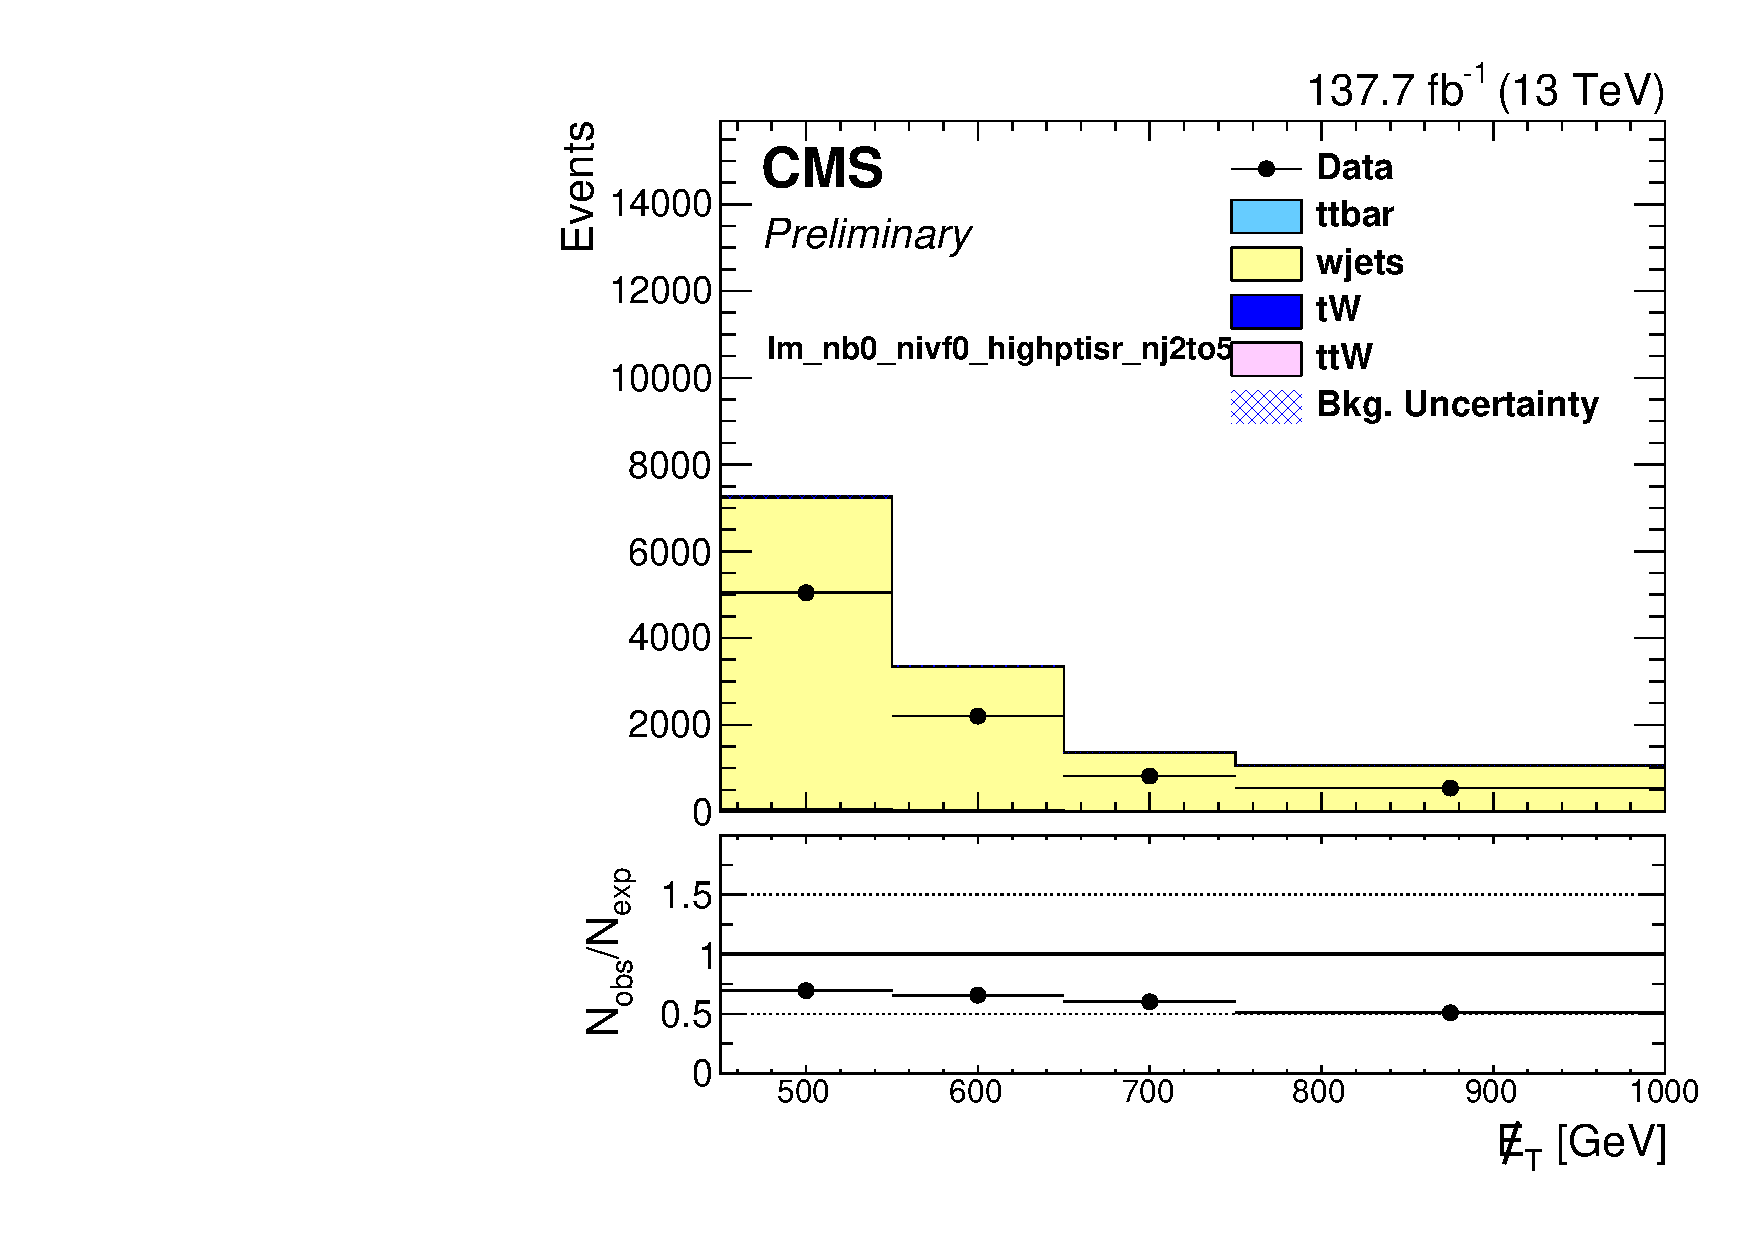
\includegraphics[width=0.49\textwidth]{lepcr_allEras/MET_pt_DataMC_lm_nb0_nivf0_highptisr_nj2to5__.pdf}
  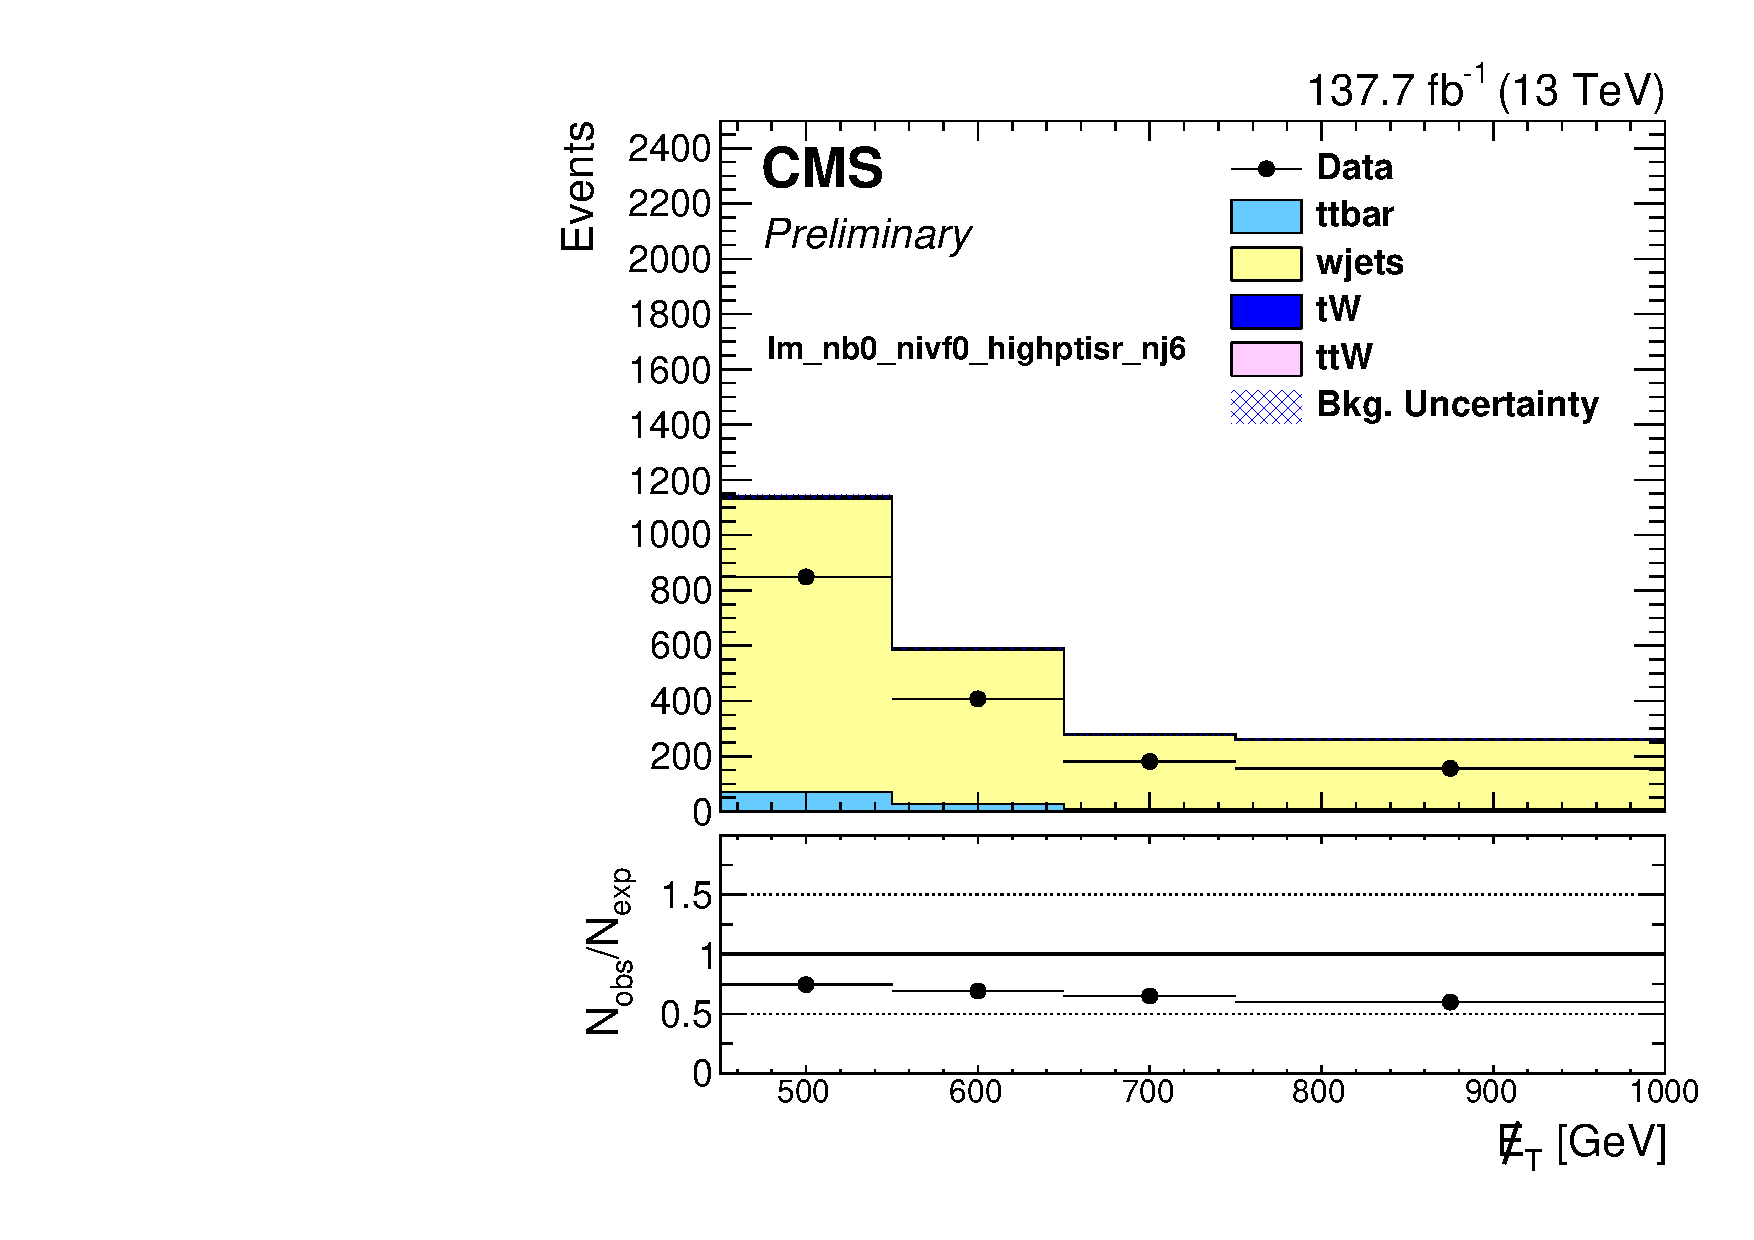
\includegraphics[width=0.49\textwidth]{lepcr_allEras/MET_pt_DataMC_lm_nb0_nivf0_highptisr_nj6__.pdf} \\
  \includegraphics[width=0.49\textwidth]{lepcr_allEras/MET_pt_DataMC_lm_nb0_nivf1_highptisr_nj2to5__.pdf}
  \includegraphics[width=0.49\textwidth]{lepcr_allEras/MET_pt_DataMC_lm_nb0_nivf1_highptisr_nj6__.pdf} \\
	\end{center}
	\caption[Lost Lepton LM Control Region $\nb=0$]{Comparison of the \met~distribution in the single-lepton sample after applying the low \dm~baseline selection in the $\nb=0$ region. Data and simulation are represented by the black points and stacked histograms, respectively. The error bars on the ratio of observed data to simulation correspond to the data statistical uncertainty and the shaded blue band represents the statistical uncertainty on the simulation. These regions are included with the search regions in the simultaneous fit for the signal extraction in order to estimate the LL contribution.
	 }
	\label{fig:llb-1lcr-datavsmc-lm-nb0}
\end{figure}
\begin{figure}[!h]
	\begin{center}  
		\includegraphics[width=0.32\textwidth]{lepcr_allEras/MET_pt_DataMC_lm_nb1_nivf0_lowmtb_lowptisr_lowptb__.pdf}
		\includegraphics[width=0.32\textwidth]{lepcr_allEras/MET_pt_DataMC_lm_nb1_nivf0_lowmtb_lowptisr_medptb__.pdf} \\
		\includegraphics[width=0.32\textwidth]{lepcr_allEras/MET_pt_DataMC_lm_nb1_nivf0_lowmtb_highptisr_lowptb__.pdf}
		\includegraphics[width=0.32\textwidth]{lepcr_allEras/MET_pt_DataMC_lm_nb1_nivf0_lowmtb_highptisr_medptb__.pdf}
		\includegraphics[width=0.32\textwidth]{lepcr_allEras/MET_pt_DataMC_lm_nb1_nivf1_lowmtb_lowptb__.pdf} \\
		\includegraphics[width=0.32\textwidth]{lepcr_allEras/MET_pt_DataMC_lm_nb2_lowmtb_lowptisr_lowptb12__.pdf} 
		\includegraphics[width=0.32\textwidth]{lepcr_allEras/MET_pt_DataMC_lm_nb2_lowmtb_lowptisr_medptb12__.pdf}
		\includegraphics[width=0.32\textwidth]{lepcr_allEras/MET_pt_DataMC_lm_nb2_lowmtb_lowptisr_highptb12_nj7__.pdf} \\
		\includegraphics[width=0.32\textwidth]{lepcr_allEras/MET_pt_DataMC_lm_nb2_lowmtb_highptisr_lowptb12__.pdf} 
		\includegraphics[width=0.32\textwidth]{lepcr_allEras/MET_pt_DataMC_lm_nb2_lowmtb_highptisr_medptb12__.pdf}
		\includegraphics[width=0.32\textwidth]{lepcr_allEras/MET_pt_DataMC_lm_nb2_lowmtb_highptisr_highptb12_nj7__.pdf} \\
	\end{center}
	\caption[Lost Lepton LM Control Region $\nb=1$]{Comparison of the \met~distribution in the single-lepton sample after applying the low \dm~baseline selection. Two top rows: Events with $\nb=1$; Two bottom rows: Events with $\nb \geq2$;  Data and simulation are represented by the black points and stacked histograms, respectively. The error bars on the ratio of observed data to simulation correspond to the data statistical uncertainty and the shaded blue band represents the statistical uncertainty on the simulation. These regions are included with the search regions in the simultaneous fit for the signal extraction in order to estimate the LL contribution.
	 }
	\label{fig:llb-1lcr-datavsmc-lm-nb1}
\end{figure}

\begin{figure}[!htb]
	\begin{center}
  \includegraphics[width=0.32\textwidth]{../Research/SUSY/2019/LLB/lepcr_allEras/MET_pt_DataMC_hm_nb1_lowmtb_nj7_nrtgeq1__.pdf}
  \includegraphics[width=0.32\textwidth]{../Research/SUSY/2019/LLB/lepcr_allEras/MET_pt_DataMC_hm_nb2_lowmtb_nj7_nrtgeq1__.pdf} \\
  \includegraphics[width=0.32\textwidth]{../Research/SUSY/2019/LLB/lepcr_allEras/MET_pt_DataMC_hm_nb1_highmtb_nj7_nt0_nrt0_nw0__.pdf}
  \includegraphics[width=0.32\textwidth]{../Research/SUSY/2019/LLB/lepcr_allEras/MET_pt_DataMC_hm_nb2_highmtb_nj7_nt0_nrt0_nw0__.pdf} \\
	\end{center}
	\caption{Comparison of the \met~distribution in the single-lepton sample after applying the high \dm~baseline selection in the $\mtb<175~\GeV$ and $\nt=0, \nrt=0,$ and $\nw=0$ region. Data and simulation are represented by the black points and stacked histograms, respectively. The error bars on the ratio of observed data to simulation correspond to the data statistical uncertainty and the shaded blue band represents the statistical uncertainty on the simulation. These regions are included with the search regions in the simultaneous fit for the signal extraction in order to estimate the LL contribution.
	 %               The plots in the top row are for events with $\mtb<175$~\GeV, with $5\leq\nj<7$ on the left and $\nj\geq7$ on the right. 
	 %               The plots in the middle row are for events with $\mtb>175$~\GeV and $\nt=0, \nw=0$, with $5\leq\nj<7$ on the left and $\nj\geq7$ on the right. 
	 %               The plot in the bottom row is for events with $\mtb>175$~\GeV and $\nj\geq5$, with $\nt=0, \nw\geq1$ on the left, $\nt\geq1, \nw=0$ on the middle, and $\nt\geq1$, and $\nw\geq1$ on the right.
	 }
	\label{fig:llb-1lcr-datavsmc-hm-nt0-nrt0-nw0}
\end{figure}

\begin{figure}[!htb]
	\begin{center}
  \includegraphics[width=0.32\textwidth]{../Research/SUSY/2019/LLB/lepcr_allEras/MET_pt_DataMC_hm_nb1_highmtb_ntgeq1_nrt0_nw0_htlt1000__.pdf}
  \includegraphics[width=0.32\textwidth]{../Research/SUSY/2019/LLB/lepcr_allEras/MET_pt_DataMC_hm_nb1_highmtb_ntgeq1_nrt0_nw0_ht1000to1500__.pdf}
  \includegraphics[width=0.32\textwidth]{../Research/SUSY/2019/LLB/lepcr_allEras/MET_pt_DataMC_hm_nb1_highmtb_ntgeq1_nrt0_nw0_htgt1500__.pdf} \\
  \includegraphics[width=0.32\textwidth]{../Research/SUSY/2019/LLB/lepcr_allEras/MET_pt_DataMC_hm_nb1_highmtb_nt0_nrt0_nwgeq1_htlt1300__.pdf} 
  \includegraphics[width=0.32\textwidth]{../Research/SUSY/2019/LLB/lepcr_allEras/MET_pt_DataMC_hm_nb1_highmtb_nt0_nrt0_nwgeq1_htgt1300__.pdf} \\
  \includegraphics[width=0.32\textwidth]{../Research/SUSY/2019/LLB/lepcr_allEras/MET_pt_DataMC_hm_nb1_highmtb_nt0_nrtgeq1_nw0_htlt1000__.pdf} 
  \includegraphics[width=0.32\textwidth]{../Research/SUSY/2019/LLB/lepcr_allEras/MET_pt_DataMC_hm_nb1_highmtb_nt0_nrtgeq1_nw0_ht1000to1500__.pdf} 
  \includegraphics[width=0.32\textwidth]{../Research/SUSY/2019/LLB/lepcr_allEras/MET_pt_DataMC_hm_nb1_highmtb_nt0_nrtgeq1_nw0_htgt1500__.pdf} \\
  \includegraphics[width=0.32\textwidth]{../Research/SUSY/2019/LLB/lepcr_allEras/MET_pt_DataMC_hm_nb1_highmtb_ntgeq1_nrt0_nwgeq1__.pdf} 
  \includegraphics[width=0.32\textwidth]{../Research/SUSY/2019/LLB/lepcr_allEras/MET_pt_DataMC_hm_nb1_highmtb_ntgeq1_nrtgeq1_nw0__.pdf} 
  \includegraphics[width=0.32\textwidth]{../Research/SUSY/2019/LLB/lepcr_allEras/MET_pt_DataMC_hm_nb1_highmtb_nt0_nrtgeq1_nwgeq1__.pdf} \\
	\end{center}
	\caption{Comparison of the \met~distribution in the single-lepton sample after applying the high \dm~baseline selection in the $\nb=1$ region where there are $\geq1$ heavy object tags. Data and simulation are represented by the black points and stacked histograms, respectively. The error bars on the ratio of observed data to simulation correspo    nd to the data statistical uncertainty and the shaded blue band represents the statistical uncertainty on the simulation. These regions are included with the search regions in the simultaneous fit for the signal extraction in order to estimate the LL contribution.
	 %               The plots in the top row are for events with $\mtb<175$~\GeV, with $5\leq\nj<7$ on the left and $\nj\geq7$ on the right. 
	 %               The plots in the middle row are for events with $\mtb>175$~\GeV and $\nt=0, \nw=0$, with $5\leq\nj<7$ on the left and $\nj\geq7$ on the right. 
	 %               The plot in the bottom row is for events with $\mtb>175$~\GeV and $\nj\geq5$, with $\nt=0, \nw\geq1$ on the left, $\nt\geq1, \nw=0$ on the middle, and $\nt\geq1$, and $\nw\geq1$ on the right.
	 }
	\label{fig:llb-1lcr-datavsmc-hm-nb1}
\end{figure}

\begin{figure}[!htb]
	\begin{center}
  \includegraphics[width=0.32\textwidth]{../Research/SUSY/2019/LLB/lepcr_allEras/MET_pt_DataMC_hm_nbeq2_highmtb_nt1_nrt0_nw0_htlt1000__.pdf}
  \includegraphics[width=0.32\textwidth]{../Research/SUSY/2019/LLB/lepcr_allEras/MET_pt_DataMC_hm_nbeq2_highmtb_nt1_nrt0_nw0_ht1000to1500__.pdf}
  \includegraphics[width=0.32\textwidth]{../Research/SUSY/2019/LLB/lepcr_allEras/MET_pt_DataMC_hm_nbeq2_highmtb_nt1_nrt0_nw0_htgt1500__.pdf} \\
  \includegraphics[width=0.32\textwidth]{../Research/SUSY/2019/LLB/lepcr_allEras/MET_pt_DataMC_hm_nbeq2_highmtb_nt0_nrt0_nw1_htlt1300__.pdf} 
  \includegraphics[width=0.32\textwidth]{../Research/SUSY/2019/LLB/lepcr_allEras/MET_pt_DataMC_hm_nbeq2_highmtb_nt0_nrt0_nw1_htgt1300__.pdf} \\
  \includegraphics[width=0.32\textwidth]{../Research/SUSY/2019/LLB/lepcr_allEras/MET_pt_DataMC_hm_nbeq2_highmtb_nt0_nrt1_nw0_htlt1000__.pdf} 
  \includegraphics[width=0.32\textwidth]{../Research/SUSY/2019/LLB/lepcr_allEras/MET_pt_DataMC_hm_nbeq2_highmtb_nt0_nrt1_nw0_ht1000to1500__.pdf} 
  \includegraphics[width=0.32\textwidth]{../Research/SUSY/2019/LLB/lepcr_allEras/MET_pt_DataMC_hm_nbeq2_highmtb_nt0_nrt1_nw0_htgt1500__.pdf} \\
  \includegraphics[width=0.32\textwidth]{../Research/SUSY/2019/LLB/lepcr_allEras/MET_pt_DataMC_hm_nbeq2_highmtb_nt1_nrt0_nw1__.pdf} 
  \includegraphics[width=0.32\textwidth]{../Research/SUSY/2019/LLB/lepcr_allEras/MET_pt_DataMC_hm_nbeq2_highmtb_nt0_nrt1_nw1__.pdf} \\
	\end{center}
	\caption{Comparison of the \met~distribution in the single-lepton sample after applying the high \dm~baseline selection in the $\nb=2$ and $\nt=1, \nrt=1,$ or $\nw=1$ regions. Data and simulation are represented by the black points and stacked histograms, respectively. The error bars on the ratio of observed data to simulation correspo    nd to the data statistical uncertainty and the shaded blue band represents the statistical uncertainty on the simulation. These regions are included with the search regions in the simultaneous fit for the signal extraction in order to estimate the LL contribution.
	 %               The plots in the top row are for events with $\mtb<175$~\GeV, with $5\leq\nj<7$ on the left and $\nj\geq7$ on the right. 
	 %               The plots in the middle row are for events with $\mtb>175$~\GeV and $\nt=0, \nw=0$, with $5\leq\nj<7$ on the left and $\nj\geq7$ on the right. 
	 %               The plot in the bottom row is for events with $\mtb>175$~\GeV and $\nj\geq5$, with $\nt=0, \nw\geq1$ on the left, $\nt\geq1, \nw=0$ on the middle, and $\nt\geq1$, and $\nw\geq1$ on the right.
	 }
	\label{fig:llb-1lcr-datavsmc-hm-nb2-1}
\end{figure}

\begin{figure}[!htb]
	\begin{center}
  \includegraphics[width=0.32\textwidth]{../Research/SUSY/2019/LLB/lepcr_allEras/MET_pt_DataMC_hm_nbeq2_highmtb_nt1_nrt1_nw0_htlt1300__.pdf}
  \includegraphics[width=0.32\textwidth]{../Research/SUSY/2019/LLB/lepcr_allEras/MET_pt_DataMC_hm_nbeq2_highmtb_nt1_nrt1_nw0_htgt1300__.pdf} \\
  \includegraphics[width=0.32\textwidth]{../Research/SUSY/2019/LLB/lepcr_allEras/MET_pt_DataMC_hm_nbeq2_highmtb_nt2_nrt0_nw0_htlt1300__.pdf}
  \includegraphics[width=0.32\textwidth]{../Research/SUSY/2019/LLB/lepcr_allEras/MET_pt_DataMC_hm_nbeq2_highmtb_nt2_nrt0_nw0_htgt1300__.pdf} 
  \includegraphics[width=0.32\textwidth]{../Research/SUSY/2019/LLB/lepcr_allEras/MET_pt_DataMC_hm_nbeq2_highmtb_nt0_nrt0_nw2__.pdf} \\
  \includegraphics[width=0.32\textwidth]{../Research/SUSY/2019/LLB/lepcr_allEras/MET_pt_DataMC_hm_nbeq2_highmtb_nt0_nrt2_nw0_htlt1300__.pdf}  
  \includegraphics[width=0.32\textwidth]{../Research/SUSY/2019/LLB/lepcr_allEras/MET_pt_DataMC_hm_nbeq2_highmtb_nt0_nrt2_nw0_htgt1300__.pdf} \\
  \includegraphics[width=0.32\textwidth]{../Research/SUSY/2019/LLB/lepcr_allEras/MET_pt_DataMC_hm_nbeq2_highmtb_nrtntnwgeq3_htlt1300__.pdf} 
  \includegraphics[width=0.32\textwidth]{../Research/SUSY/2019/LLB/lepcr_allEras/MET_pt_DataMC_hm_nbeq2_highmtb_nrtntnwgeq3_htgt1300__.pdf} \\
	\end{center}
	\caption{Comparison of the \met~distribution in the single-lepton sample after applying the high \dm~baseline selection in the $\nb=2$ and $\nt=2, \nrt=2,$ or $\nw=2$ region. Data and simulation are represented by the black points and stacked histograms, respectively. The error bars on the ratio of observed data to simulation correspo    nd to the data statistical uncertainty and the shaded blue band represents the statistical uncertainty on the simulation. These regions are included with the search regions in the simultaneous fit for the signal extraction in order to estimate the LL contribution.
	 %               The plots in the top row are for events with $\mtb<175$~\GeV, with $5\leq\nj<7$ on the left and $\nj\geq7$ on the right. 
	 %               The plots in the middle row are for events with $\mtb>175$~\GeV and $\nt=0, \nw=0$, with $5\leq\nj<7$ on the left and $\nj\geq7$ on the right. 
	 %               The plot in the bottom row is for events with $\mtb>175$~\GeV and $\nj\geq5$, with $\nt=0, \nw\geq1$ on the left, $\nt\geq1, \nw=0$ on the middle, and $\nt\geq1$, and $\nw\geq1$ on the right.
	 }
	\label{fig:llb-1lcr-datavsmc-hm-nb2-2}
\end{figure}

\begin{figure}[!htb]
	\begin{center}
  \includegraphics[width=0.32\textwidth]{../Research/SUSY/2019/LLB/lepcr_allEras/MET_pt_DataMC_hm_nb3_highmtb_nt1_nrt0_nw0_htlt1000__.pdf}
  \includegraphics[width=0.32\textwidth]{../Research/SUSY/2019/LLB/lepcr_allEras/MET_pt_DataMC_hm_nb3_highmtb_nt1_nrt0_nw0_ht1000to1500__.pdf} 
  \includegraphics[width=0.32\textwidth]{../Research/SUSY/2019/LLB/lepcr_allEras/MET_pt_DataMC_hm_nb3_highmtb_nt1_nrt0_nw0_htgt1500__.pdf} \\
  \includegraphics[width=0.32\textwidth]{../Research/SUSY/2019/LLB/lepcr_allEras/MET_pt_DataMC_hm_nb3_highmtb_nt0_nrt0_nw1__.pdf} 
  \includegraphics[width=0.32\textwidth]{../Research/SUSY/2019/LLB/lepcr_allEras/MET_pt_DataMC_hm_nb3_highmtb_nt0_nrt1_nw0_htlt1000__.pdf} \\
  \includegraphics[width=0.32\textwidth]{../Research/SUSY/2019/LLB/lepcr_allEras/MET_pt_DataMC_hm_nb3_highmtb_nt0_nrt1_nw0_ht1000to1500__.pdf}  
  \includegraphics[width=0.32\textwidth]{../Research/SUSY/2019/LLB/lepcr_allEras/MET_pt_DataMC_hm_nb3_highmtb_nt0_nrt1_nw0_htgt1500__.pdf} \\
  \includegraphics[width=0.32\textwidth]{../Research/SUSY/2019/LLB/lepcr_allEras/MET_pt_DataMC_hm_nb3_highmtb_nt1_nrt0_nw1__.pdf} 
  \includegraphics[width=0.32\textwidth]{../Research/SUSY/2019/LLB/lepcr_allEras/MET_pt_DataMC_hm_nb3_highmtb_nt0_nrt1_nw1__.pdf} \\
	\end{center}
	\caption{Comparison of the \met~distribution in the single-lepton sample after applying the high \dm~baseline selection in the $\nb\geq3$ and $\nt=1, \nrt=1,$ or $\nw=1$ region. Data and simulation are represented by the black points and stacked histograms, respectively. The error bars on the ratio of observed data to simulation correspo    nd to the data statistical uncertainty and the shaded blue band represents the statistical uncertainty on the simulation. These regions are included with the search regions in the simultaneous fit for the signal extraction in order to estimate the LL contribution.
	 %               The plots in the top row are for events with $\mtb<175$~\GeV, with $5\leq\nj<7$ on the left and $\nj\geq7$ on the right. 
	 %               The plots in the middle row are for events with $\mtb>175$~\GeV and $\nt=0, \nw=0$, with $5\leq\nj<7$ on the left and $\nj\geq7$ on the right. 
	 %               The plot in the bottom row is for events with $\mtb>175$~\GeV and $\nj\geq5$, with $\nt=0, \nw\geq1$ on the left, $\nt\geq1, \nw=0$ on the middle, and $\nt\geq1$, and $\nw\geq1$ on the right.
	 }
	\label{fig:llb-1lcr-datavsmc-hm-nb3-1}
\end{figure}

\begin{figure}[!htb]
	\begin{center}
  \includegraphics[width=0.32\textwidth]{../Research/SUSY/2019/LLB/lepcr_allEras/MET_pt_DataMC_hm_nb3_highmtb_nt1_nrt1_nw0_htlt1300__.pdf} 
  \includegraphics[width=0.32\textwidth]{../Research/SUSY/2019/LLB/lepcr_allEras/MET_pt_DataMC_hm_nb3_highmtb_nt1_nrt1_nw0_htgt1300__.pdf} \\  
  \includegraphics[width=0.32\textwidth]{../Research/SUSY/2019/LLB/lepcr_allEras/MET_pt_DataMC_hm_nb3_highmtb_nt2_nrt0_nw0_htlt1300__.pdf} 
  \includegraphics[width=0.32\textwidth]{../Research/SUSY/2019/LLB/lepcr_allEras/MET_pt_DataMC_hm_nb3_highmtb_nt2_nrt0_nw0_htgt1300__.pdf} 
  \includegraphics[width=0.32\textwidth]{../Research/SUSY/2019/LLB/lepcr_allEras/MET_pt_DataMC_hm_nb3_highmtb_nt0_nrt0_nw2__.pdf} \\
  \includegraphics[width=0.32\textwidth]{../Research/SUSY/2019/LLB/lepcr_allEras/MET_pt_DataMC_hm_nb3_highmtb_nt0_nrt2_nw0_htlt1300__.pdf} 
  \includegraphics[width=0.32\textwidth]{../Research/SUSY/2019/LLB/lepcr_allEras/MET_pt_DataMC_hm_nb3_highmtb_nt0_nrt2_nw0_htgt1300__.pdf} 
  \includegraphics[width=0.32\textwidth]{../Research/SUSY/2019/LLB/lepcr_allEras/MET_pt_DataMC_hm_nb3_highmtb_nrtntnwgeq3__.pdf} \\
	\end{center}
	\caption{Comparison of the \met~distribution in the single-lepton sample after applying the high \dm~baseline selection in the $\nb\geq3$ $\nt=2, \nrt=2,$ or $\nw=2$ region. Data and simulation are represented by the black points and stacked histograms, respectively. The error bars on the ratio of observed data to simulation correspo    nd to the data statistical uncertainty and the shaded blue band represents the statistical uncertainty on the simulation. These regions are included with the search regions in the simultaneous fit for the signal extraction in order to estimate the LL contribution.
	 %               The plots in the top row are for events with $\mtb<175$~\GeV, with $5\leq\nj<7$ on the left and $\nj\geq7$ on the right. 
	 %               The plots in the middle row are for events with $\mtb>175$~\GeV and $\nt=0, \nw=0$, with $5\leq\nj<7$ on the left and $\nj\geq7$ on the right. 
	 %               The plot in the bottom row is for events with $\mtb>175$~\GeV and $\nj\geq5$, with $\nt=0, \nw\geq1$ on the left, $\nt\geq1, \nw=0$ on the middle, and $\nt\geq1$, and $\nw\geq1$ on the right.
	 }
	\label{fig:llb-1lcr-datavsmc-hm-nb3-2}
\end{figure}


Now that we have confirmed that the LL background is valid to be combined to be combined for all the eras. The transfer factors and control region comparisons confirm that each era can be combined in the final estimation. Now with the combinations of each era for the LL back ground, we can consider the combination of the other background estimations. 

\section{Z Boson Decay to Neutrinos}
\label{sec:Znunu}

An important source of background for the zero-lepton search is from events in which a \Z{} boson decays to neutrinos. Since neutrinos are weakly interacting the are missed by the CMS detector which results in \met. Two methods are traditionally used to estimate the \Znunu{} background. The first method makes use of a sample dominated by \Zll+jets events which has similar kinematics, but has much lower statistics in the tight search regions. The second method utilizes a $\gamma+$jets sample which has a factor of 5 or more large cross section and similar leading Feynman diagrams. The main differences are quark-boson couplings and the fact that the \Z{} boson is very massive. In the realm of the analysis, where events have large boson \pt{} these effects become less important. The \met{} of the $\gamma+$jets process is calculated after removing the photon from the event to mimic the \Znunu{} process.

We use a hybrid method to estimate the \Znunu{} background that makes use of both the $\gamma+$jets and the \Zll+jets processes. The photon and the dilepton system are removed from the events before calculating \met{} and other kinematic variables related to \met, and the modified \met{} is denoted by $\met^\gamma$ and $\met^{ll}$ for $\gamma+$jets and the \Zll+jets processes, respectively. The \Zll+jets sample is used to measure the normalization of the \Znunu{} process in different ranges of \nb{} and \nsv, and we take advantage of the much higher statistics of the $\gamma+$jets sample to extract shape corrections. 

\subsection{Prediction Method}\label{subsec:znunupred}

The prediction of the \Znunu{} background is given by:
\begin{equation}
N_{pred}^{\Znunu}=N_{MC}^{\Znunu} \cdot R_Z \cdot S_\gamma
\end{equation}
where $N_{MC}^{\Znunu}$ is the expected number of \Znunu{} events obtained from simulation in a given search region, $R_Z$ is a factor used to account for any difference betweeen data and simulation in the cross-section of the \Znunu{} process, $S_\gamma$ accounts for any shape difference in the \Znunu{} process between data and simulation and is integrated in top and W tags. We use the same extrapolation method, see sec. \ref{sec:LL}, for the CR-to-SR transfer factor. The merged bins in $t$ and $W$ tags increases the limited statistics in these regions. 

The factor $R_Z$ is calculated by comparing the observed and expected \Zll{} yields after applying a relaxed definition of the baseline selection, with the $\Delta\phi(j,\met^{ll})$ cut removed. The purity of the sample in improved by requiring the dilepton invariant mass to be near the \Z-mass window $(80<M_{ll}<100$ GeV) with a $\pt>200$ Gev cut for the entire system. Unfortunately the \ttbar{} contamination is not negligible in the $\nb\geq1$ region. To account for this we define a factor $R_T$ for \ttbar{} events which is calculated by using events outside the \Z-mass window $(50<M_{ll}<80$ or $M_{ll}>100$ GeV). The relation between the factors, $R_Z$ and $R_T$, and the observed and expected yields inside and outside the Z-mass window, 
\begin{equation}
\begin{bmatrix}
\text{Data}_{\text{on}-Z} \\
\text{Data}_{\text{off}-Z}
\end{bmatrix}
=
\begin{bmatrix}
\text{MC}_{\text{on}-Z}(\Zll) & MC_{\text{on}-Z}(\ttbar) \\
\text{MC}_{\text{off}-Z}(\Zll) & MC_{\text{off}-Z}(\ttbar)
\end{bmatrix}
\cdot
\begin{bmatrix}
R_Z \\
R_T
\end{bmatrix}.
\end{equation}
The small contributions from $tZ, ttZ, WZ,$ and $ZZ$ and included in $R_Z$, while the processes $tW, ttW,$ and $WW$ are included in $R_T$. 

%To account for potential effects related to heavy flavor production, $R_Z$ and $R_T$ are calculated separately for different \nb{} and \nsv{} requirements. The high and low \dm{} baseline selections are applied for the corresponding regions, except for the requirements on the azimuthal angles between the leading jets and \met. Figures ? to ? show the data and simulated events in the regions used to calculate $R_Z$ and $R_T$, and results are summarized in Table ?. The statistical uncertainties on $R_Z$ are included in the systematic uncertainty on the final background prediction. 

%We utilize the $\gamma$+jets sample to extract corrections related to the modeling of the kinematics of \Znunu+jets events. The selected $\gamma$+jets sample consists of events that have at least one photon satisfying the selection described in Section 3.11. The quantity $S_\gamma$ is the shape correction factor that is calculated via a comparison of the $\met^\gamma$ distributions of $\gamma$+jets events in simulation and data. The simulation is normalized to the number of events seen in data after applying the baseline selections corresponding to the low and high \dm{} searches, respectively. A different $S_\gamma$ is estimated for each search region, to account for effects related to the search variables, and is used to correct the corresponding \Znunu+jets yields from simulation. To increase the statistical power of the correction, in the low \dm{} regions, we integrate over \nsv{} for $\nb=0$ and $\nb=1$ separately after verifying in simulation that there is no bias introduced in $\gamma$+jets $\met^\gamma$ distributions.

\subsection{Combination of Eras}\label{subsec:znunucombine}

We want to make sure that the normalization and shape corrections in the electron and muon control regions are in relative aggreement to be able to combine them into a single normalization and shape correction. Figure \ref{fig:znunu-norm-lm-elec} and \ref{fig:znunu-norm-lm-muon} compare the normalized $\met^\gamma$ distributions for $\gamma$+jets in data and simulation in each separate low \dm{} control region and eras of the analysis. A comparison between the electron and muon control regions and the combinations is shown in Fig. \ref{fig:znunu-norm-lm-comp} and \ref{fig:znunu-norm-hm-comp}. The shape agreement is in good agreement between each era so we are able to combine them all together. In fig. \ref{fig:znunu-shape-lm-photon}, we have the shape correction in the low \dm{} photon control region separated into each era. Each of the eras are in good agreement so we should be able to combine all of the eras for each part of the analysis together.

\begin{figure}[!h]
	\begin{center}
    \includegraphics[width=0.3\textwidth]{znunu/fromCaleb/DataMC_Muon_LowDM_bestRecoZM_50to250_jetpt30_2016.png}
    \includegraphics[width=0.3\textwidth]{znunu/fromCaleb/DataMC_Muon_LowDM_bestRecoZM_50to250_jetpt30_2017_BE.png} \\
    \includegraphics[width=0.3\textwidth]{znunu/fromCaleb/DataMC_Muon_LowDM_bestRecoZM_50to250_jetpt30_2017_F.png}
    \includegraphics[width=0.3\textwidth]{znunu/fromCaleb/DataMC_Muon_LowDM_bestRecoZM_50to250_jetpt30_2018_PreHEM.png}
    \includegraphics[width=0.3\textwidth]{znunu/fromCaleb/DataMC_Muon_LowDM_bestRecoZM_50to250_jetpt30_2018_PostHEM.png}
	\end{center}
	\caption[\Znunu{} Normalization in low \dm{} for muons]{The \Znunu{} normalization separated by era for the muon control region. The selection is the low $\dm, \nb=0, \nsv=0$ in the muon control region.
	 }
	\label{fig:znunu-norm-lm-muon}
\end{figure}

\begin{figure}[!h]
	\begin{center}
    \includegraphics[width=0.3\textwidth]{znunu/fromCaleb/DataMC_Muon_HighDM_bestRecoZM_50to250_jetpt30_2016.png}
    \includegraphics[width=0.3\textwidth]{znunu/fromCaleb/DataMC_Muon_HighDM_bestRecoZM_50to250_jetpt30_2017_BE.png} \\
    \includegraphics[width=0.3\textwidth]{znunu/fromCaleb/DataMC_Muon_HighDM_bestRecoZM_50to250_jetpt30_2017_F.png}
    \includegraphics[width=0.3\textwidth]{znunu/fromCaleb/DataMC_Muon_HighDM_bestRecoZM_50to250_jetpt30_2018_PreHEM.png}
    \includegraphics[width=0.3\textwidth]{znunu/fromCaleb/DataMC_Muon_HighDM_bestRecoZM_50to250_jetpt30_2018_PostHEM.png}
	\end{center}
	\caption[\Znunu{} Normalization in high \dm{} for muons]{The \Znunu{} normalization separated by era for the muon control region. The selection is the high $\dm, \nb=1, =2, \geq2,\geq3$ in the muon control region.
	 }
	\label{fig:znunu-norm-hm-muon}
\end{figure}

\begin{figure}[!h]
	\begin{center}
    \includegraphics[width=0.3\textwidth]{znunu/fromCaleb/DataMC_Electron_LowDM_bestRecoZM_50to250_jetpt30_2016.png}
    \includegraphics[width=0.3\textwidth]{znunu/fromCaleb/DataMC_Electron_LowDM_bestRecoZM_50to250_jetpt30_2017_BE.png} \\
    \includegraphics[width=0.3\textwidth]{znunu/fromCaleb/DataMC_Electron_LowDM_bestRecoZM_50to250_jetpt30_2017_F.png}
    \includegraphics[width=0.3\textwidth]{znunu/fromCaleb/DataMC_Electron_LowDM_bestRecoZM_50to250_jetpt30_2018_PreHEM.png}
    \includegraphics[width=0.3\textwidth]{znunu/fromCaleb/DataMC_Electron_LowDM_bestRecoZM_50to250_jetpt30_2018_PostHEM.png}
	\end{center}
	\caption[\Znunu{} Normalization in low \dm{} for electronss]{The \Znunu{} normalization separated by era for the electron control region. The selection is the low $\dm, \nb=0, \nsv=0$ in the electron control region.
	 }
	\label{fig:znunu-norm-lm-electron}
\end{figure}

\begin{figure}[!h]
	\begin{center}
    \includegraphics[width=0.3\textwidth]{znunu/fromCaleb/DataMC_Electron_HighDM_bestRecoZM_50to250_jetpt30_2016.png}
    \includegraphics[width=0.3\textwidth]{znunu/fromCaleb/DataMC_Electron_HighDM_bestRecoZM_50to250_jetpt30_2017_BE.png} \\
    \includegraphics[width=0.3\textwidth]{znunu/fromCaleb/DataMC_Electron_HighDM_bestRecoZM_50to250_jetpt30_2017_F.png}
    \includegraphics[width=0.3\textwidth]{znunu/fromCaleb/DataMC_Electron_HighDM_bestRecoZM_50to250_jetpt30_2018_PreHEM.png}
    \includegraphics[width=0.3\textwidth]{znunu/fromCaleb/DataMC_Electron_HighDM_bestRecoZM_50to250_jetpt30_2018_PostHEM.png}
	\end{center}
	\caption[\Znunu{} Normalization in high \dm{} for electrons]{The \Znunu{} normalization separated by era for the electron control region. The selection is the high $\dm, \nb=1, =2, \geq2,\geq3$ in the electron control region.
	 }
	\label{fig:znunu-norm-hm-electron}
\end{figure}

\begin{figure}[!h]
	\begin{center}
  \includegraphics[width=0.3\textwidth]{znunu/fromCaleb/DataMC_Photon_LowDM_met_jetpt30_2016.png}
  \includegraphics[width=0.3\textwidth]{znunu/fromCaleb/DataMC_Photon_LowDM_met_jetpt30_2017_BE.png} \\
  \includegraphics[width=0.3\textwidth]{znunu/fromCaleb/DataMC_Photon_LowDM_met_jetpt30_2017_F.png}
  \includegraphics[width=0.3\textwidth]{znunu/fromCaleb/DataMC_Photon_LowDM_met_jetpt30_2018_PreHEM.png}
  \includegraphics[width=0.3\textwidth]{znunu/fromCaleb/DataMC_Photon_LowDM_met_jetpt30_2018_PostHEM.png}
	\end{center}
	\caption[\Znunu{} Shape by Era]{The \Znunu{} shape corrections separated by era for the low \dm{} control region. The selection is the low $\dm, \nb=0, 2\leq\nj\leq5$ in the photon control region.
	 }
	\label{fig:znunu-shape-lm-photon}
\end{figure}

\begin{figure}[!h]
	\begin{center}
  \includegraphics[width=0.3\textwidth]{znunu/fromCaleb/DataMC_Photon_HighDM_met_jetpt30_2016.png}
  \includegraphics[width=0.3\textwidth]{znunu/fromCaleb/DataMC_Photon_HighDM_met_jetpt30_2017_BE.png} \\
  \includegraphics[width=0.3\textwidth]{znunu/fromCaleb/DataMC_Photon_HighDM_met_jetpt30_2017_F.png}
  \includegraphics[width=0.3\textwidth]{znunu/fromCaleb/DataMC_Photon_HighDM_met_jetpt30_2018_PreHEM.png}
  \includegraphics[width=0.3\textwidth]{znunu/fromCaleb/DataMC_Photon_HighDM_met_jetpt30_2018_PostHEM.png}
	\end{center}
	\caption[\Znunu{} Shape by Era]{The \Znunu{} shape corrections separated by era for the high \dm{} control region. The selection is the low $\dm, \nb=0, 2\leq\nj\leq5$ in the photon control region.
	 }
	\label{fig:znunu-shape-hm-photon}
\end{figure}

\begin{figure}[!h]
	\begin{center}
  \includegraphics[width=0.40\textwidth]{znunu/znunu_norm_lm_comp_nb0_nsv0.png} \\
  \includegraphics[width=0.40\textwidth]{znunu/znunu_norm_lm_comp_nb0_nsv1.png} 
  \includegraphics[width=0.40\textwidth]{znunu/znunu_norm_lm_comp_nb1_nsv0.png} \\
  \includegraphics[width=0.40\textwidth]{znunu/znunu_norm_lm_comp_nb1_nsv1.png} 
  \includegraphics[width=0.40\textwidth]{znunu/znunu_norm_lm_comp_nb2.png} \\

	\end{center}
	\caption[\Znunu{} Normalization Low \dm{} Comparisons]{The \Znunu{} normalization comparisons for each era in the electron and muon control region for different regions in the low $\dm, \nb=0,=1,\geq2, \nsv=0,\geq1$.
	 }
	\label{fig:znunu-norm-lm-comp}
\end{figure}

\begin{figure}[!h]
	\begin{center}
  \includegraphics[width=0.49\textwidth]{znunu/znunu_norm_hm_comp_nb1.png}
  \includegraphics[width=0.49\textwidth]{znunu/znunu_norm_hm_comp_nb2.png} \\
  \includegraphics[width=0.49\textwidth]{znunu/znunu_norm_hm_comp_nbgeq2.png}
  \includegraphics[width=0.49\textwidth]{znunu/znunu_norm_hm_comp_nbgeq3.png} \\
	\end{center}
	\caption[\Znunu{} Normalization High \dm{} Comparisons]{The \Znunu{} normalization comparisons for each era in the electron and muon control region for different regions in the high $\dm, \nb=1,=2,\geq2, \text{ and } \geq3$.
	 }
	\label{fig:znunu-norm-hm-comp}
\end{figure}


\subsection{Prediction}\label{subsec:znunuprediction}

%The events are selected online using the HLT\_Photon165\_HE10 trigger. The photon trigger efficiency is observed to degrade by up to ~ 10\% at high photon \pt{} due to an inefficiency in the L1 trigger. We therefore utilize the combination of triggers listed in Table 1 to recover efficiency. To suppress potential signal contamination and ensure that the control sample is independent from the search sample, we only consider events with $\met<200$ GeV. The $\gamma$+jets data control sample consists of three main components: prompt photons produced directly or via fragmentation, and fake photons. We combine the $\gamma$+jets and QCD simulated samples to estimate the contributions of these components to our control sample. We consider prompt photons to be reconstructed photons that are matched to a generator-level photon in space and momentum as follows: $\Delta R(\gamma_{gen}, \gamma_{reco})<0.1$ and $0.5<\pt^{gen}/\pt^reco<2$. We use the $\gamma$+jets simulation to describe the direct photon component and the QCD simulation to describe the fragmentation and fake components. We consider direct photons to be those that satisfy the relationship $\Delta R(\gamma, \text{parton})>0.4$, where parton refers to a quark of gluon at the generator level. To avoid double-counting events from the $\gamma$+jets and QCD simulated samples, we reject events in the QCD sample with $\Delta R(\gamma,\text{parton})>0.4$. Finally, reconstructed photons that are not matched to a generator-level photon are considered to be fakes. Finally, the $\gamma$+jets sample can also have a sizable contribution from $tt\gamma$ events in regions requiring at least one top- or W- have shown that significant variations in the normalization of each of these components in the $\gamma$+jets sample do not significantly affect the shapes of the search region variable distributions, and therefore it is sufficient to estimate the relative contributions of each component using the simulated samples. 

Table \ref{table:zinv_search} summarize the yields of the \Znunu{} background in each search region along with the prediction after including the shape and renormalization factors. 

{
\footnotesize
\tabcolsep=0.01cm
\centering
\begin{longtable}{|p{0.05\textwidth}|p{0.5\textwidth}|*2{p{0.2\textwidth}|}}
\hline Bin & Selection & $N_{MC}$ & $N_{p}$ \\
\hline 0 & $\mathrm{Low}~\Delta m, N_{b} = 0, N_{sv} = 0, N_{j} \leq 5$, $450 \leq \met < 550$ & $7256.263 \pm 19.884$ & $5208.311 \pm 76.401$ \\
\hline 1 & $\mathrm{Low}~\Delta m, N_{b} = 0, N_{sv} = 0, N_{j} \leq 5$, $550 \leq \met < 650$ & $5411.438 \pm 14.579$ & $3526.854 \pm 60.845$ \\
\hline 2 & $\mathrm{Low}~\Delta m, N_{b} = 0, N_{sv} = 0, N_{j} \leq 5$, $650 \leq \met < 750$ & $2671.714 \pm 8.082$ & $1640.922 \pm 36.527$ \\
\hline 3 & $\mathrm{Low}~\Delta m, N_{b} = 0, N_{sv} = 0, N_{j} \leq 5$, $\met \geq 750$ & $2628.838 \pm 8.373$ & $1435.498 \pm 37.419$ \\
\hline 4 & $\mathrm{Low}~\Delta m, N_{b} = 0, N_{sv} = 0, N_{j} \geq 6$, $450 \leq \met < 550$ & $142.274 \pm 1.975$ & $109.280 \pm 6.374$ \\
\hline 5 & $\mathrm{Low}~\Delta m, N_{b} = 0, N_{sv} = 0, N_{j} \geq 6$, $550 \leq \met < 650$ & $92.175 \pm 1.562$ & $67.417 \pm 5.987$ \\
\hline 6 & $\mathrm{Low}~\Delta m, N_{b} = 0, N_{sv} = 0, N_{j} \geq 6$, $650 \leq \met < 750$ & $53.798 \pm 1.197$ & $49.864 \pm 5.190$ \\
\hline 7 & $\mathrm{Low}~\Delta m, N_{b} = 0, N_{sv} = 0, N_{j} \geq 6$, $\met \geq 750$ & $70.683 \pm 1.421$ & $45.003 \pm 5.664$ \\
\hline 8 & $\mathrm{Low}~\Delta m, N_{b} = 0, N_{sv} \geq 1, N_{j} \leq 5$, $450 \leq \met < 550$ & $212.081 \pm 3.384$ & $122.858 \pm 6.501$ \\
\hline 9 & $\mathrm{Low}~\Delta m, N_{b} = 0, N_{sv} \geq 1, N_{j} \leq 5$, $550 \leq \met < 650$ & $160.857 \pm 2.554$ & $84.854 \pm 4.589$ \\
\hline 10 & $\mathrm{Low}~\Delta m, N_{b} = 0, N_{sv} \geq 1, N_{j} \leq 5$, $650 \leq \met < 750$ & $83.583 \pm 1.497$ & $41.669 \pm 2.377$ \\
\hline 11 & $\mathrm{Low}~\Delta m, N_{b} = 0, N_{sv} \geq 1, N_{j} \leq 5$, $\met \geq 750$ & $78.561 \pm 1.513$ & $34.971 \pm 2.074$ \\
\hline 12 & $\mathrm{Low}~\Delta m, N_{b} = 0, N_{sv} \geq 1, N_{j} \geq 6$, $450 \leq \met < 550$ & $4.999 \pm 0.381$ & $3.141 \pm 0.339$ \\
\hline 13 & $\mathrm{Low}~\Delta m, N_{b} = 0, N_{sv} \geq 1, N_{j} \geq 6$, $550 \leq \met < 650$ & $2.894 \pm 0.291$ & $1.788 \pm 0.256$ \\
\hline 14 & $\mathrm{Low}~\Delta m, N_{b} = 0, N_{sv} \geq 1, N_{j} \geq 6$, $650 \leq \met < 750$ & $1.642 \pm 0.242$ & $1.293 \pm 0.247$ \\
\hline 15 & $\mathrm{Low}~\Delta m, N_{b} = 0, N_{sv} \geq 1, N_{j} \geq 6$, $\met \geq 750$ & $2.840 \pm 0.294$ & $1.510 \pm 0.259$ \\
\hline 16 & $\mathrm{Low}~\Delta m, N_{b} = 1, N_{sv} = 0$, $300 \leq \met < 400$ & $985.010 \pm 11.471$ & $994.981 \pm 44.192$ \\
\hline 17 & $\mathrm{Low}~\Delta m, N_{b} = 1, N_{sv} = 0$, $400 \leq \met < 500$ & $234.210 \pm 4.993$ & $212.599 \pm 12.399$ \\
\hline 18 & $\mathrm{Low}~\Delta m, N_{b} = 1, N_{sv} = 0$, $500 \leq \met < 600$ & $27.269 \pm 1.151$ & $23.612 \pm 2.169$ \\
\hline 19 & $\mathrm{Low}~\Delta m, N_{b} = 1, N_{sv} = 0$, $\met \geq 600$ & $5.843 \pm 0.392$ & $5.567 \pm 0.666$ \\
\hline 20 & $\mathrm{Low}~\Delta m, N_{b} = 1, N_{sv} = 0$, $300 \leq \met < 400$ & $416.933 \pm 7.066$ & $420.647 \pm 19.396$ \\
\hline 21 & $\mathrm{Low}~\Delta m, N_{b} = 1, N_{sv} = 0$, $400 \leq \met < 500$ & $77.689 \pm 2.660$ & $71.123 \pm 4.579$ \\
\hline 22 & $\mathrm{Low}~\Delta m, N_{b} = 1, N_{sv} = 0$, $500 \leq \met < 600$ & $7.063 \pm 0.444$ & $6.177 \pm 0.632$ \\
\hline 23 & $\mathrm{Low}~\Delta m, N_{b} = 1, N_{sv} = 0$, $\met \geq 600$ & $1.448 \pm 0.181$ & $1.371 \pm 0.220$ \\
\hline 24 & $\mathrm{Low}~\Delta m, N_{b} = 1, N_{sv} = 0$, $450 \leq \met < 550$ & $89.469 \pm 2.246$ & $83.374 \pm 5.664$ \\
\hline 25 & $\mathrm{Low}~\Delta m, N_{b} = 1, N_{sv} = 0$, $550 \leq \met < 650$ & $43.078 \pm 1.145$ & $34.743 \pm 3.843$ \\
\hline 26 & $\mathrm{Low}~\Delta m, N_{b} = 1, N_{sv} = 0$, $650 \leq \met < 750$ & $22.023 \pm 0.772$ & $23.572 \pm 3.910$ \\
\hline 27 & $\mathrm{Low}~\Delta m, N_{b} = 1, N_{sv} = 0$, $\met \geq 750$ & $16.925 \pm 0.685$ & $19.063 \pm 3.716$ \\
\hline 28 & $\mathrm{Low}~\Delta m, N_{b} = 1, N_{sv} = 0$, $450 \leq \met < 550$ & $43.452 \pm 1.485$ & $40.451 \pm 2.916$ \\
\hline 29 & $\mathrm{Low}~\Delta m, N_{b} = 1, N_{sv} = 0$, $550 \leq \met < 650$ & $17.811 \pm 0.669$ & $14.281 \pm 1.632$ \\
\hline 30 & $\mathrm{Low}~\Delta m, N_{b} = 1, N_{sv} = 0$, $650 \leq \met < 750$ & $7.014 \pm 0.425$ & $7.328 \pm 1.250$ \\
\hline 31 & $\mathrm{Low}~\Delta m, N_{b} = 1, N_{sv} = 0$, $\met \geq 750$ & $6.412 \pm 0.425$ & $7.164 \pm 1.469$ \\
\hline 32 & $\mathrm{Low}~\Delta m, N_{b} = 1, N_{sv} \geq 1$, $300 \leq \met < 400$ & $71.110 \pm 3.266$ & $47.063 \pm 9.630$ \\
\hline 33 & $\mathrm{Low}~\Delta m, N_{b} = 1, N_{sv} \geq 1$, $400 \leq \met < 500$ & $19.866 \pm 1.270$ & $11.198 \pm 2.441$ \\
\hline 34 & $\mathrm{Low}~\Delta m, N_{b} = 1, N_{sv} \geq 1$, $\met \geq 500$ & $12.494 \pm 0.755$ & $7.547 \pm 1.621$ \\
\hline 35 & $\mathrm{Low}~\Delta m, N_{b} \geq 2$, $300 \leq \met < 400$ & $65.112 \pm 2.836$ & $62.074 \pm 9.733$ \\
\hline 36 & $\mathrm{Low}~\Delta m, N_{b} \geq 2$, $400 \leq \met < 500$ & $17.910 \pm 1.404$ & $13.174 \pm 2.841$ \\
\hline 37 & $\mathrm{Low}~\Delta m, N_{b} \geq 2$, $\met \geq 500$ & $4.292 \pm 0.849$ & $3.364 \pm 0.935$ \\
\hline 38 & $\mathrm{Low}~\Delta m, N_{b} \geq 2$, $300 \leq \met < 400$ & $78.522 \pm 2.758$ & $76.869 \pm 11.902$ \\
\hline 39 & $\mathrm{Low}~\Delta m, N_{b} \geq 2$, $400 \leq \met < 500$ & $19.902 \pm 1.252$ & $14.495 \pm 3.120$ \\
\hline 40 & $\mathrm{Low}~\Delta m, N_{b} \geq 2$, $\met \geq 500$ & $2.641 \pm 0.266$ & $2.409 \pm 0.544$ \\
\hline 41 & $\mathrm{Low}~\Delta m, N_{b} \geq 2, N_{j} \geq 7$, $300 \leq \met < 400$ & $1.938 \pm 0.256$ & $7.399 \pm 14.091$ \\
\hline 42 & $\mathrm{Low}~\Delta m, N_{b} \geq 2, N_{j} \geq 7$, $400 \leq \met < 500$ & $0.576 \pm 0.111$ & $-1.796 \pm 3.170$ \\
\hline 43 & $\mathrm{Low}~\Delta m, N_{b} \geq 2, N_{j} \geq 7$, $\met \geq 500$ & $0.220 \pm 0.070$ & $-1.288 \pm 2.305$ \\
\hline 44 & $\mathrm{Low}~\Delta m, N_{b} \geq 2$, $450 \leq \met < 550$ & $5.117 \pm 0.354$ & $3.551 \pm 0.824$ \\
\hline 45 & $\mathrm{Low}~\Delta m, N_{b} \geq 2$, $550 \leq \met < 650$ & $4.043 \pm 0.307$ & $3.292 \pm 0.950$ \\
\hline 46 & $\mathrm{Low}~\Delta m, N_{b} \geq 2$, $\met \geq 650$ & $2.714 \pm 0.251$ & $4.148 \pm 1.290$ \\
\hline 47 & $\mathrm{Low}~\Delta m, N_{b} \geq 2$, $450 \leq \met < 550$ & $8.715 \pm 0.498$ & $6.463 \pm 1.423$ \\
\hline 48 & $\mathrm{Low}~\Delta m, N_{b} \geq 2$, $550 \leq \met < 650$ & $4.707 \pm 0.409$ & $3.786 \pm 1.087$ \\
\hline 49 & $\mathrm{Low}~\Delta m, N_{b} \geq 2$, $\met \geq 650$ & $3.214 \pm 0.277$ & $5.198 \pm 1.662$ \\
\hline 50 & $\mathrm{Low}~\Delta m, N_{b} \geq 2, N_{j} \geq 7$, $450 \leq \met < 550$ & $0.557 \pm 0.130$ & $1.364 \pm 1.139$ \\
\hline 51 & $\mathrm{Low}~\Delta m, N_{b} \geq 2, N_{j} \geq 7$, $550 \leq \met < 650$ & $0.267 \pm 0.083$ & $0.437 \pm 0.471$ \\
\hline 52 & $\mathrm{Low}~\Delta m, N_{b} \geq 2, N_{j} \geq 7$, $\met \geq 650$ & $0.354 \pm 0.109$ & $-5.232 \pm 8.317$ \\
\hline 53 & $\mathrm{High}~\Delta m, N_{b} = 1, N_{j} \geq 7$, $250 \leq \met < 300$ & $7.227 \pm 0.671$ & $8.161 \pm 1.731$ \\
\hline 54 & $\mathrm{High}~\Delta m, N_{b} = 1, N_{j} \geq 7$, $300 \leq \met < 400$ & $4.664 \pm 0.414$ & $5.827 \pm 0.930$ \\
\hline 55 & $\mathrm{High}~\Delta m, N_{b} = 1, N_{j} \geq 7$, $400 \leq \met < 500$ & $1.115 \pm 0.157$ & $1.762 \pm 0.340$ \\
\hline 56 & $\mathrm{High}~\Delta m, N_{b} = 1, N_{j} \geq 7$, $\met \geq 500$ & $1.175 \pm 0.212$ & $1.397 \pm 0.355$ \\
\hline 57 & $\mathrm{High}~\Delta m, N_{b} \geq 2, N_{j} \geq 7$, $250 \leq \met < 300$ & $7.040 \pm 0.666$ & $9.220 \pm 2.070$ \\
\hline 58 & $\mathrm{High}~\Delta m, N_{b} \geq 2, N_{j} \geq 7$, $300 \leq \met < 400$ & $5.418 \pm 0.606$ & $7.500 \pm 1.538$ \\
\hline 59 & $\mathrm{High}~\Delta m, N_{b} \geq 2, N_{j} \geq 7$, $400 \leq \met < 500$ & $1.436 \pm 0.175$ & $2.244 \pm 0.536$ \\
\hline 60 & $\mathrm{High}~\Delta m, N_{b} \geq 2, N_{j} \geq 7$, $\met \geq 500$ & $0.907 \pm 0.140$ & $0.799 \pm 0.279$ \\
\hline 61 & $\mathrm{High}~\Delta m, N_{b} = 1$, $250 \leq \met < 350$ & $174.544 \pm 2.195$ & $219.327 \pm 15.411$ \\
\hline 62 & $\mathrm{High}~\Delta m, N_{b} = 1$, $350 \leq \met < 450$ & $101.459 \pm 1.665$ & $130.446 \pm 6.753$ \\
\hline 63 & $\mathrm{High}~\Delta m, N_{b} = 1$, $450 \leq \met < 550$ & $62.139 \pm 1.323$ & $83.367 \pm 5.201$ \\
\hline 64 & $\mathrm{High}~\Delta m, N_{b} = 1$, $\met \geq 550$ & $120.674 \pm 1.875$ & $140.392 \pm 8.978$ \\
\hline 65 & $\mathrm{High}~\Delta m, N_{b} \geq 2$, $250 \leq \met < 350$ & $26.815 \pm 0.850$ & $35.406 \pm 3.703$ \\
\hline 66 & $\mathrm{High}~\Delta m, N_{b} \geq 2$, $350 \leq \met < 450$ & $18.766 \pm 0.698$ & $23.182 \pm 2.581$ \\
\hline 67 & $\mathrm{High}~\Delta m, N_{b} \geq 2$, $450 \leq \met < 550$ & $12.745 \pm 0.588$ & $15.712 \pm 2.105$ \\
\hline 68 & $\mathrm{High}~\Delta m, N_{b} \geq 2$, $\met \geq 550$ & $23.555 \pm 0.795$ & $22.626 \pm 3.261$ \\
\hline 69 & $\mathrm{High}~\Delta m, N_{b} = 1$, $250 \leq \met < 550$ & $22.898 \pm 1.171$ & $29.511 \pm 2.094$ \\
\hline 70 & $\mathrm{High}~\Delta m, N_{b} = 1$, $550 \leq \met < 650$ & $3.399 \pm 0.336$ & $4.569 \pm 0.595$ \\
\hline 71 & $\mathrm{High}~\Delta m, N_{b} = 1$, $\met \geq 650$ & $2.112 \pm 0.233$ & $2.178 \pm 0.306$ \\
\hline 72 & $\mathrm{High}~\Delta m, N_{b} = 1$, $250 \leq \met < 550$ & $8.321 \pm 0.471$ & $10.788 \pm 0.835$ \\
\hline 73 & $\mathrm{High}~\Delta m, N_{b} = 1$, $550 \leq \met < 650$ & $0.917 \pm 0.156$ & $1.137 \pm 0.227$ \\
\hline 74 & $\mathrm{High}~\Delta m, N_{b} = 1$, $\met \geq 650$ & $1.693 \pm 0.223$ & $1.715 \pm 0.276$ \\
\hline 75 & $\mathrm{High}~\Delta m, N_{b} = 1$, $250 \leq \met < 550$ & $2.397 \pm 0.263$ & $3.017 \pm 0.388$ \\
\hline 76 & $\mathrm{High}~\Delta m, N_{b} = 1$, $550 \leq \met < 650$ & $0.237 \pm 0.080$ & $0.267 \pm 0.095$ \\
\hline 77 & $\mathrm{High}~\Delta m, N_{b} = 1$, $\met \geq 650$ & $0.382 \pm 0.121$ & $0.375 \pm 0.130$ \\
\hline 78 & $\mathrm{High}~\Delta m, N_{b} = 1$, $250 \leq \met < 350$ & $17.309 \pm 0.921$ & $19.688 \pm 2.408$ \\
\hline 79 & $\mathrm{High}~\Delta m, N_{b} = 1$, $350 \leq \met < 450$ & $9.976 \pm 0.860$ & $11.894 \pm 1.263$ \\
\hline 80 & $\mathrm{High}~\Delta m, N_{b} = 1$, $\met \geq 450$ & $5.631 \pm 0.383$ & $6.236 \pm 0.607$ \\
\hline 81 & $\mathrm{High}~\Delta m, N_{b} = 1$, $250 \leq \met < 350$ & $1.235 \pm 0.179$ & $1.401 \pm 0.260$ \\
\hline 82 & $\mathrm{High}~\Delta m, N_{b} = 1$, $350 \leq \met < 450$ & $0.563 \pm 0.115$ & $0.641 \pm 0.141$ \\
\hline 83 & $\mathrm{High}~\Delta m, N_{b} = 1$, $\met \geq 450$ & $0.746 \pm 0.135$ & $0.807 \pm 0.164$ \\
\hline 84 & $\mathrm{High}~\Delta m, N_{b} = 1$, $250 \leq \met < 350$ & $195.175 \pm 4.837$ & $251.383 \pm 16.983$ \\
\hline 85 & $\mathrm{High}~\Delta m, N_{b} = 1$, $350 \leq \met < 450$ & $74.884 \pm 2.420$ & $97.067 \pm 5.751$ \\
\hline 86 & $\mathrm{High}~\Delta m, N_{b} = 1$, $450 \leq \met < 550$ & $26.313 \pm 1.155$ & $34.960 \pm 2.636$ \\
\hline 87 & $\mathrm{High}~\Delta m, N_{b} = 1$, $550 \leq \met < 650$ & $10.278 \pm 0.501$ & $13.003 \pm 1.193$ \\
\hline 88 & $\mathrm{High}~\Delta m, N_{b} = 1$, $\met \geq 650$ & $5.139 \pm 0.356$ & $4.945 \pm 0.565$ \\
\hline 89 & $\mathrm{High}~\Delta m, N_{b} = 1$, $250 \leq \met < 350$ & $8.008 \pm 0.446$ & $10.110 \pm 0.929$ \\
\hline 90 & $\mathrm{High}~\Delta m, N_{b} = 1$, $350 \leq \met < 450$ & $5.178 \pm 0.363$ & $6.583 \pm 0.575$ \\
\hline 91 & $\mathrm{High}~\Delta m, N_{b} = 1$, $450 \leq \met < 550$ & $3.186 \pm 0.286$ & $4.299 \pm 0.478$ \\
\hline 92 & $\mathrm{High}~\Delta m, N_{b} = 1$, $550 \leq \met < 650$ & $2.187 \pm 0.237$ & $2.741 \pm 0.381$ \\
\hline 93 & $\mathrm{High}~\Delta m, N_{b} = 1$, $\met \geq 650$ & $3.978 \pm 0.324$ & $4.073 \pm 0.485$ \\
\hline 94 & $\mathrm{High}~\Delta m, N_{b} = 1$, $250 \leq \met < 350$ & $1.434 \pm 0.206$ & $1.735 \pm 0.295$ \\
\hline 95 & $\mathrm{High}~\Delta m, N_{b} = 1$, $350 \leq \met < 450$ & $0.902 \pm 0.163$ & $1.163 \pm 0.226$ \\
\hline 96 & $\mathrm{High}~\Delta m, N_{b} = 1$, $450 \leq \met < 550$ & $0.615 \pm 0.131$ & $0.822 \pm 0.189$ \\
\hline 97 & $\mathrm{High}~\Delta m, N_{b} = 1$, $550 \leq \met < 650$ & $0.288 \pm 0.083$ & $0.298 \pm 0.091$ \\
\hline 98 & $\mathrm{High}~\Delta m, N_{b} = 1$, $\met \geq 650$ & $1.129 \pm 0.173$ & $1.008 \pm 0.193$ \\
\hline 99 & $\mathrm{High}~\Delta m, N_{b} = 1$, $250 \leq \met < 550$ & $0.110 \pm 0.048$ & $0.112 \pm 0.051$ \\
\hline 100 & $\mathrm{High}~\Delta m, N_{b} = 1$, $\met \geq 550$ & $0.001 \pm 0.002$ & $0.001 \pm 0.002$ \\
\hline 101 & $\mathrm{High}~\Delta m, N_{b} = 1$, $250 \leq \met < 550$ & $0.398 \pm 0.102$ & $0.479 \pm 0.129$ \\
\hline 102 & $\mathrm{High}~\Delta m, N_{b} = 1$, $\met \geq 550$ & $0.260 \pm 0.081$ & $0.307 \pm 0.106$ \\
\hline 103 & $\mathrm{High}~\Delta m, N_{b} = 1$, $250 \leq \met < 550$ & $1.145 \pm 0.290$ & $1.374 \pm 0.400$ \\
\hline 104 & $\mathrm{High}~\Delta m, N_{b} = 1$, $\met \geq 550$ & $0.118 \pm 0.046$ & $0.114 \pm 0.047$ \\
\hline 105 & $\mathrm{High}~\Delta m, N_{b} = 2$, $250 \leq \met < 550$ & $6.792 \pm 0.557$ & $8.638 \pm 1.096$ \\
\hline 106 & $\mathrm{High}~\Delta m, N_{b} = 2$, $550 \leq \met < 650$ & $1.649 \pm 0.580$ & $1.514 \pm 0.611$ \\
\hline 107 & $\mathrm{High}~\Delta m, N_{b} = 2$, $\met \geq 650$ & $0.786 \pm 0.140$ & $0.855 \pm 0.230$ \\
\hline 108 & $\mathrm{High}~\Delta m, N_{b} = 2$, $250 \leq \met < 550$ & $2.581 \pm 0.256$ & $3.281 \pm 0.454$ \\
\hline 109 & $\mathrm{High}~\Delta m, N_{b} = 2$, $550 \leq \met < 650$ & $0.201 \pm 0.066$ & $0.186 \pm 0.069$ \\
\hline 110 & $\mathrm{High}~\Delta m, N_{b} = 2$, $\met \geq 650$ & $0.608 \pm 0.117$ & $0.587 \pm 0.161$ \\
\hline 111 & $\mathrm{High}~\Delta m, N_{b} = 2$, $250 \leq \met < 550$ & $0.289 \pm 0.083$ & $0.359 \pm 0.109$ \\
\hline 112 & $\mathrm{High}~\Delta m, N_{b} = 2$, $550 \leq \met < 650$ & $0.102 \pm 0.058$ & $0.092 \pm 0.055$ \\
\hline 113 & $\mathrm{High}~\Delta m, N_{b} = 2$, $\met \geq 650$ & $0.253 \pm 0.084$ & $0.282 \pm 0.117$ \\
\hline 114 & $\mathrm{High}~\Delta m, N_{b} = 2$, $250 \leq \met < 350$ & $2.668 \pm 0.351$ & $3.328 \pm 0.584$ \\
\hline 115 & $\mathrm{High}~\Delta m, N_{b} = 2$, $350 \leq \met < 450$ & $1.094 \pm 0.175$ & $1.241 \pm 0.274$ \\
\hline 116 & $\mathrm{High}~\Delta m, N_{b} = 2$, $\met \geq 450$ & $1.024 \pm 0.150$ & $1.073 \pm 0.217$ \\
\hline 117 & $\mathrm{High}~\Delta m, N_{b} = 2$, $250 \leq \met < 350$ & $0.060 \pm 0.036$ & $0.070 \pm 0.044$ \\
\hline 118 & $\mathrm{High}~\Delta m, N_{b} = 2$, $350 \leq \met < 450$ & $0.138 \pm 0.053$ & $0.153 \pm 0.066$ \\
\hline 119 & $\mathrm{High}~\Delta m, N_{b} = 2$, $\met \geq 450$ & $0.069 \pm 0.036$ & $0.069 \pm 0.038$ \\
\hline 120 & $\mathrm{High}~\Delta m, N_{b} = 2$, $250 \leq \met < 350$ & $50.003 \pm 2.431$ & $65.511 \pm 7.190$ \\
\hline 121 & $\mathrm{High}~\Delta m, N_{b} = 2$, $350 \leq \met < 450$ & $21.195 \pm 1.350$ & $24.494 \pm 3.139$ \\
\hline 122 & $\mathrm{High}~\Delta m, N_{b} = 2$, $450 \leq \met < 550$ & $6.467 \pm 0.494$ & $7.814 \pm 1.257$ \\
\hline 123 & $\mathrm{High}~\Delta m, N_{b} = 2$, $550 \leq \met < 650$ & $3.162 \pm 0.285$ & $2.865 \pm 0.614$ \\
\hline 124 & $\mathrm{High}~\Delta m, N_{b} = 2$, $\met \geq 650$ & $1.199 \pm 0.159$ & $1.325 \pm 0.322$ \\
\hline 125 & $\mathrm{High}~\Delta m, N_{b} = 2$, $250 \leq \met < 350$ & $1.885 \pm 0.205$ & $2.449 \pm 0.367$ \\
\hline 126 & $\mathrm{High}~\Delta m, N_{b} = 2$, $350 \leq \met < 450$ & $1.374 \pm 0.182$ & $1.625 \pm 0.286$ \\
\hline 127 & $\mathrm{High}~\Delta m, N_{b} = 2$, $450 \leq \met < 550$ & $0.996 \pm 0.153$ & $1.166 \pm 0.239$ \\
\hline 128 & $\mathrm{High}~\Delta m, N_{b} = 2$, $550 \leq \met < 650$ & $0.776 \pm 0.141$ & $0.700 \pm 0.184$ \\
\hline 129 & $\mathrm{High}~\Delta m, N_{b} = 2$, $\met \geq 650$ & $0.906 \pm 0.140$ & $0.901 \pm 0.233$ \\
\hline 130 & $\mathrm{High}~\Delta m, N_{b} = 2$, $250 \leq \met < 350$ & $0.398 \pm 0.103$ & $0.535 \pm 0.155$ \\
\hline 131 & $\mathrm{High}~\Delta m, N_{b} = 2$, $350 \leq \met < 450$ & $0.247 \pm 0.081$ & $0.275 \pm 0.098$ \\
\hline 132 & $\mathrm{High}~\Delta m, N_{b} = 2$, $450 \leq \met < 550$ & $0.395 \pm 0.110$ & $0.461 \pm 0.143$ \\
\hline 133 & $\mathrm{High}~\Delta m, N_{b} = 2$, $550 \leq \met < 650$ & $0.098 \pm 0.046$ & $0.092 \pm 0.051$ \\
\hline 134 & $\mathrm{High}~\Delta m, N_{b} = 2$, $\met \geq 650$ & $0.275 \pm 0.086$ & $0.299 \pm 0.131$ \\
\hline 135 & $\mathrm{High}~\Delta m, N_{b} = 2$, $250 \leq \met < 550$ & $0.026 \pm 0.026$ & $0.030 \pm 0.030$ \\
\hline 136 & $\mathrm{High}~\Delta m, N_{b} = 2$, $\met \geq 550$ & $0.026 \pm 0.025$ & $0.022 \pm 0.022$ \\
\hline 137 & $\mathrm{High}~\Delta m, N_{b} = 2$, $250 \leq \met < 350$ & $0.051 \pm 0.030$ & $0.064 \pm 0.038$ \\
\hline 138 & $\mathrm{High}~\Delta m, N_{b} = 2$, $350 \leq \met < 450$ & $0.111 \pm 0.050$ & $0.138 \pm 0.064$ \\
\hline 139 & $\mathrm{High}~\Delta m, N_{b} = 2$, $\met \geq 450$ & $0.177 \pm 0.077$ & $0.206 \pm 0.096$ \\
\hline 140 & $\mathrm{High}~\Delta m, N_{b} = 2$, $250 \leq \met < 350$ & $0.008 \pm 0.009$ & $0.010 \pm 0.010$ \\
\hline 141 & $\mathrm{High}~\Delta m, N_{b} = 2$, $350 \leq \met < 450$ & $0.027 \pm 0.027$ & $0.031 \pm 0.032$ \\
\hline 142 & $\mathrm{High}~\Delta m, N_{b} = 2$, $\met \geq 450$ & $0.090 \pm 0.049$ & $0.095 \pm 0.053$ \\
\hline 143 & $\mathrm{High}~\Delta m, N_{b} = 2$, $250 \leq \met < 550$ & $0.212 \pm 0.066$ & $0.252 \pm 0.086$ \\
\hline 144 & $\mathrm{High}~\Delta m, N_{b} = 2$, $\met \geq 550$ & $0.035 \pm 0.027$ & $0.027 \pm 0.021$ \\
\hline 145 & $\mathrm{High}~\Delta m, N_{b} = 2$, $250 \leq \met < 450$ & $0.000 \pm 0.002$ & $0.000 \pm 0.002$ \\
\hline 146 & $\mathrm{High}~\Delta m, N_{b} = 2$, $\met \geq 450$ & $0.000 \pm 0.002$ & $0.000 \pm 0.002$ \\
\hline 147 & $\mathrm{High}~\Delta m, N_{b} = 2$, $\met \geq 250$ & $0.019 \pm 0.020$ & $0.022 \pm 0.023$ \\
\hline 148 & $\mathrm{High}~\Delta m, N_{b} = 2$, $250 \leq \met < 450$ & $0.657 \pm 0.203$ & $0.831 \pm 0.293$ \\
\hline 149 & $\mathrm{High}~\Delta m, N_{b} = 2$, $\met \geq 450$ & $0.190 \pm 0.068$ & $0.198 \pm 0.076$ \\
\hline 150 & $\mathrm{High}~\Delta m, N_{b} = 2$, $250 \leq \met < 450$ & $0.000 \pm 0.002$ & $0.000 \pm 0.002$ \\
\hline 151 & $\mathrm{High}~\Delta m, N_{b} = 2$, $\met \geq 450$ & $0.019 \pm 0.019$ & $0.019 \pm 0.019$ \\
\hline 152 & $\mathrm{High}~\Delta m, N_{b} = 2$, $\met \geq 250$ & $0.000 \pm 0.002$ & $0.000 \pm 0.002$ \\
\hline 153 & $\mathrm{High}~\Delta m, N_{b} \geq 3$, $250 \leq \met < 350$ & $0.175 \pm 0.054$ & $0.308 \pm 0.211$ \\
\hline 154 & $\mathrm{High}~\Delta m, N_{b} \geq 3$, $350 \leq \met < 550$ & $0.276 \pm 0.080$ & $0.566 \pm 0.301$ \\
\hline 155 & $\mathrm{High}~\Delta m, N_{b} \geq 3$, $\met \geq 550$ & $0.340 \pm 0.096$ & $0.235 \pm 0.167$ \\
\hline 156 & $\mathrm{High}~\Delta m, N_{b} \geq 3$, $250 \leq \met < 350$ & $0.152 \pm 0.063$ & $0.212 \pm 0.170$ \\
\hline 157 & $\mathrm{High}~\Delta m, N_{b} \geq 3$, $350 \leq \met < 550$ & $0.221 \pm 0.071$ & $0.397 \pm 0.206$ \\
\hline 158 & $\mathrm{High}~\Delta m, N_{b} \geq 3$, $\met \geq 550$ & $0.238 \pm 0.088$ & $0.213 \pm 0.152$ \\
\hline 159 & $\mathrm{High}~\Delta m, N_{b} \geq 3$, $250 \leq \met < 350$ & $0.057 \pm 0.039$ & $0.034 \pm 0.092$ \\
\hline 160 & $\mathrm{High}~\Delta m, N_{b} \geq 3$, $350 \leq \met < 550$ & $0.000 \pm 0.002$ & $0.000 \pm 0.002$ \\
\hline 161 & $\mathrm{High}~\Delta m, N_{b} \geq 3$, $\met \geq 550$ & $0.063 \pm 0.046$ & $0.038 \pm 0.047$ \\
\hline 162 & $\mathrm{High}~\Delta m, N_{b} \geq 3$, $250 \leq \met < 350$ & $0.232 \pm 0.074$ & $0.355 \pm 0.228$ \\
\hline 163 & $\mathrm{High}~\Delta m, N_{b} \geq 3$, $350 \leq \met < 550$ & $0.234 \pm 0.083$ & $0.079 \pm 0.125$ \\
\hline 164 & $\mathrm{High}~\Delta m, N_{b} \geq 3$, $\met \geq 550$ & $0.027 \pm 0.018$ & $0.020 \pm 0.021$ \\
\hline 165 & $\mathrm{High}~\Delta m, N_{b} \geq 3$, $250 \leq \met < 350$ & $3.020 \pm 0.452$ & $4.522 \pm 2.638$ \\
\hline 166 & $\mathrm{High}~\Delta m, N_{b} \geq 3$, $350 \leq \met < 550$ & $2.826 \pm 0.428$ & $6.297 \pm 2.829$ \\
\hline 167 & $\mathrm{High}~\Delta m, N_{b} \geq 3$, $\met \geq 550$ & $0.195 \pm 0.065$ & $0.353 \pm 0.257$ \\
\hline 168 & $\mathrm{High}~\Delta m, N_{b} \geq 3$, $250 \leq \met < 350$ & $0.399 \pm 0.096$ & $0.717 \pm 0.365$ \\
\hline 169 & $\mathrm{High}~\Delta m, N_{b} \geq 3$, $350 \leq \met < 550$ & $0.217 \pm 0.066$ & $0.415 \pm 0.218$ \\
\hline 170 & $\mathrm{High}~\Delta m, N_{b} \geq 3$, $\met \geq 550$ & $0.348 \pm 0.093$ & $0.482 \pm 0.311$ \\
\hline 171 & $\mathrm{High}~\Delta m, N_{b} \geq 3$, $250 \leq \met < 350$ & $0.054 \pm 0.035$ & $0.079 \pm 0.069$ \\
\hline 172 & $\mathrm{High}~\Delta m, N_{b} \geq 3$, $350 \leq \met < 550$ & $0.035 \pm 0.024$ & $0.056 \pm 0.057$ \\
\hline 173 & $\mathrm{High}~\Delta m, N_{b} \geq 3$, $\met \geq 550$ & $0.032 \pm 0.028$ & $0.016 \pm 0.022$ \\
\hline 174 & $\mathrm{High}~\Delta m, N_{b} \geq 3$, $\met \geq 250$ & $0.022 \pm 0.022$ & $0.023 \pm 0.027$ \\
\hline 175 & $\mathrm{High}~\Delta m, N_{b} \geq 3$, $250 \leq \met < 350$ & $0.001 \pm 0.002$ & $0.000 \pm 0.002$ \\
\hline 176 & $\mathrm{High}~\Delta m, N_{b} \geq 3$, $\met \geq 350$ & $0.142 \pm 0.051$ & $0.390 \pm 0.197$ \\
\hline 177 & $\mathrm{High}~\Delta m, N_{b} \geq 3$, $\met \geq 250$ & $0.000 \pm 0.002$ & $0.000 \pm 0.002$ \\
\hline 178 & $\mathrm{High}~\Delta m, N_{b} \geq 3$, $\met \geq 250$ & $0.038 \pm 0.028$ & $0.050 \pm 0.057$ \\
\hline 179 & $\mathrm{High}~\Delta m, N_{b} \geq 3$, $\met \geq 250$ & $0.000 \pm 0.002$ & $0.000 \pm 0.002$ \\
\hline 180 & $\mathrm{High}~\Delta m, N_{b} \geq 3$, $250 \leq \met < 350$ & $0.018 \pm 0.018$ & $0.027 \pm 0.031$ \\
\hline 181 & $\mathrm{High}~\Delta m, N_{b} \geq 3$, $\met \geq 350$ & $0.023 \pm 0.014$ & $0.049 \pm 0.043$ \\
\hline 182 & $\mathrm{High}~\Delta m, N_{b} \geq 3$, $\met \geq 250$ & $0.000 \pm 0.002$ & $0.000 \pm 0.002$ \\
\hline
\caption{Z Invisible Total Prediction for Search Bins (Run2)}
% WARNING: do not delete label
\label{table:zinv_search}
\end{longtable}
}

% matches pred table
% copy and paste the output from the end of ZnunuPred() (it calls printMoriond17Table) between the below labels "start insert" and "stop insert".
\begin{table}[!h]
\begin{center}
\resizebox*{0.6\textwidth}{!}{
\begin{tabular}{|c||c||c|c|c|c|c|}
\hline
Search Region & \met [GeV] & $N_{MC}^{\Znunu}$ & $N_{\text{pred}}^{\Znunu}$ \\
\hline
\hline
\multicolumn{4}{c}{high \dm, $\nb=1$, $\mtb<175$~\GeV, $\nj\geq7$, $\nrt\geq1$} \\
\hline
 %      hm_nb1_lowmtb_nj7_nrtgeq1
53  & $250-300$ 	& $7.227 \pm 0.671$ & $8.161 \pm 1.731$ \\
54  & $300-400$ 	& $4.664 \pm 0.414$ & $5.827 \pm 0.930$ \\
55  & $400-500$ 	& $1.115 \pm 0.157$ & $1.762 \pm 0.340$ \\
56  & $\geq 500$ 	& $1.175 \pm 0.212$ & $1.397 \pm 0.355$ \\
\hline
\multicolumn{4}{c}{high \dm, $\nb\geq2$, $\mtb<175$~\GeV, $\nj\geq7$, $\nrt\geq1$} \\
\hline
 %      hm_nb2_lowmtb_nj7_nrtgeq1
57  & $250-300$ 	& $7.040 \pm 0.666$ & $9.220 \pm 2.070$ \\
58  & $300-400$ 	& $5.418 \pm 0.606$ & $7.500 \pm 1.538$ \\
59  & $400-500$ 	& $1.436 \pm 0.175$ & $2.244 \pm 0.536$ \\
60  & $\geq 500$ 	& $0.907 \pm 0.140$ & $0.799 \pm 0.279$ \\
\hline
\multicolumn{4}{c}{high \dm, $\nb=1$, $\mtb\geq175$~\GeV, $\nt=0$, $\nrt=0$, $\nw=0$, $\Ht\geq1000$} \\
\hline
 % hm_nb1_highmtb_nt0_nrt0_nw0_htgt1000
61  & $250-350$ 	& $174.544 \pm 2.195$ & $219.327 \pm 15.411$ \\
62  & $350-450$ 	& $101.459 \pm 1.665$ & $130.446 \pm 6.753$ \\
63  & $450-550$ 	& $62.139 \pm 1.323$ & $83.367 \pm 5.201$ \\
64  & $\geq 550$ 	& $120.674 \pm 1.875$ & $140.392 \pm 8.978$ \\
\hline
\multicolumn{4}{c}{high \dm, $\nb\geq2$, $\mtb\geq175$~\GeV, $\nt=0$, $\nrt=0$, $\nw=0$, $\Ht\geq1000$} \\
\hline
 % hm_nb2_highmtb_nt0_nrt0_nw0_htgt1000
65  & $250-350$ 	& $26.815 \pm 0.850$ & $35.406 \pm 3.703$ \\
66  & $350-450$ 	& $18.766 \pm 0.698$ & $23.182 \pm 2.581$ \\
67  & $450-550$ 	& $12.745 \pm 0.588$ & $15.712 \pm 2.105$ \\
68  & $\geq 550$ 	& $23.555 \pm 0.795$ & $22.626 \pm 3.261$ \\
\hline
\multicolumn{4}{c}{high \dm, $\nb=1$, $\mtb\geq175$~\GeV, $\nt\geq1$, $\nrt=0$, $\nw=0$, $\Ht<1000$} \\
\hline
 % hm_nb1_highmtb_ntgeq1_nrt0_nw0_htlt1000
69  & $250-550$ 	& $22.898 \pm 1.171$ & $29.511 \pm 2.094$ \\
70  & $550-650$ 	& $3.399 \pm 0.336$ & $4.569 \pm 0.595$ \\
71  & $\geq 650$ 	& $2.112 \pm 0.233$ & $2.178 \pm 0.306$ \\
\hline
\multicolumn{4}{c}{high \dm, $\nb=1$, $\mtb\geq175$~\GeV, $\nt\geq1$, $\nrt=0$, $\nw=0$, $1000\leq\Ht<1500$} \\
\hline
 % hm_nb1_highmtb_ntgeq1_nrt0_nw0_ht1000to1500
72  & $250-550$ 	& $8.321 \pm 0.471$ & $10.788 \pm 0.835$ \\
73  & $550-650$ 	& $0.917 \pm 0.156$ & $1.137 \pm 0.227$ \\
74  & $\geq 650$ 	& $1.693 \pm 0.223$ & $1.715 \pm 0.276$ \\
\hline
\multicolumn{4}{c}{high \dm, $\nb=1$, $\mtb\geq175$~\GeV, $\nt\geq1$, $\nrt=0$, $\nw=0$, $\Ht\geq1500$} \\
\hline
 % hm_nb1_highmtb_ntgeq1_nrt0_nw0_htgt1500
75  & $250-550$ 	& $2.397 \pm 0.263$ & $3.017 \pm 0.388$ \\
76  & $550-650$ 	& $0.237 \pm 0.080$ & $0.267 \pm 0.095$ \\
77  & $\geq 650$ 	& $0.382 \pm 0.121$ & $0.375 \pm 0.130$ \\
\hline
\multicolumn{4}{c}{high \dm, $\nb=1$, $\mtb\geq175$~\GeV, $\nt=0$, $\nrt=0$, $\nw\geq1$, $\Ht<1300$} \\
\hline
 % hm_nb1_highmtb_nt0_nrt0_nwgeq1_htlt1300
78  & $250-350$ 	& $17.309 \pm 0.921$ & $19.688 \pm 2.408$ \\
79  & $350-450$ 	& $9.976 \pm 0.860$ & $11.894 \pm 1.263$ \\
80  & $\geq 450$ 	& $5.631 \pm 0.383$ & $6.236 \pm 0.607$ \\
\hline
\multicolumn{4}{c}{high \dm, $\nb=1$, $\mtb\geq175$~\GeV, $\nt=0$, $\nrt=0$, $\nw\geq1$, $\Ht\geq1300$} \\
\hline
 % hm_nb1_highmtb_nt0_nrt0_nwgeq1_htgt1300
81  & $250-350$ 	& $1.235 \pm 0.179$ & $1.401 \pm 0.260$ \\
82  & $350-450$ 	& $0.563 \pm 0.115$ & $0.641 \pm 0.141$ \\
83  & $\geq 450$ 	& $0.746 \pm 0.135$ & $0.807 \pm 0.164$ \\
\hline
\multicolumn{4}{c}{high \dm, $\nb=1$, $\mtb\geq175$~\GeV, $\nt=0$, $\nrt\geq1$, $\nw=0$, $\Ht<1000$} \\
\hline
 % hm_nb1_highmtb_nt0_nrtgeq1_nw0_htlt1000
84  & $250-350$ 	& $195.175 \pm 4.837$ & $251.383 \pm 16.983$ \\
85  & $350-450$ 	& $74.884 \pm 2.420$ & $97.067 \pm 5.751$ \\
86  & $450-550$ 	& $26.313 \pm 1.155$ & $34.960 \pm 2.636$ \\
87  & $550-650$ 	& $10.278 \pm 0.501$ & $13.003 \pm 1.193$ \\
88  & $\geq 650$ 	& $5.139 \pm 0.356$ & $4.945 \pm 0.565$ \\
\hline
\multicolumn{4}{c}{high \dm, $\nb=1$, $\mtb\geq175$~\GeV, $\nt=0$, $\nrt\geq1$, $\nw=0$, $1000\leq\Ht<1500$} \\
\hline
 % hm_nb1_highmtb_nt0_nrtgeq1_nw0_ht1000to1500
89  & $250-350$ 	& $8.008 \pm 0.446$ & $10.110 \pm 0.929$ \\
90  & $350-450$ 	& $5.178 \pm 0.363$ & $6.583 \pm 0.575$ \\
91  & $450-550$ 	& $3.186 \pm 0.286$ & $4.299 \pm 0.478$ \\
92  & $550-650$ 	& $2.187 \pm 0.237$ & $2.741 \pm 0.381$ \\
93  & $\geq 650$ 	& $3.978 \pm 0.324$ & $4.073 \pm 0.485$ \\
\hline
\end{tabular}
}
\caption[\Znunu{} HM CR bins 53-93]{\label{tab:0l-zinv-pred-hm-1}The \Znunu{} estimate in the various high \dm{} search regions, bins 53 to 93, using the \datalumi~dataset.}
\end{center}
\end{table}
% matches pred table
% copy and paste the output from the end of ZnunuPred() (it calls printMoriond17Table) between the below labels "start insert" and "stop insert".
\begin{table}[!h]
\begin{center}
\resizebox*{0.6\textwidth}{!}{
\begin{tabular}{|c||c||c|c|c|c|c|}
\hline
Search Region & \met [GeV] & $N_{MC}^{\Znunu}$ & $N_{\text{pred}}^{\Znunu}$ \\
\hline
\multicolumn{4}{c}{high \dm, $\nb=1$, $\mtb\geq175$~\GeV, $\nt=0$, $\nrt\geq1$, $\nw=0$, $\Ht\geq1500$} \\
\hline
 % hm_nb1_highmtb_nt0_nrtgeq1_nw0_htgt1500
94  & $250-350$ 	& $1.434 \pm 0.206$ & $1.735 \pm 0.295$ \\
95  & $350-450$ 	& $0.902 \pm 0.163$ & $1.163 \pm 0.226$ \\
96  & $450-550$ 	& $0.615 \pm 0.131$ & $0.822 \pm 0.189$ \\
97  & $550-650$ 	& $0.288 \pm 0.083$ & $0.298 \pm 0.091$ \\
98  & $\geq 650$ 	& $1.129 \pm 0.173$ & $1.008 \pm 0.193$ \\
\hline
\multicolumn{4}{c}{high \dm, $\nb=1$, $\mtb\geq175$~\GeV, $\nt\geq1$, $\nrt=0$, $\nw\geq1$} \\
\hline
 % hm_nb1_highmtb_ntgeq1_nrt0_nwgeq1
99  & $250-550$ 	& $0.110 \pm 0.048$ & $0.112 \pm 0.051$ \\
100 & $\geq 550$ 	& $0.001 \pm 0.002$ & $0.001 \pm 0.002$ \\
\hline
\multicolumn{4}{c}{high \dm, $\nb=1$, $\mtb\geq175$~\GeV, $\nt\geq1$, $\nrt\geq1$, $\nw=0$} \\
\hline
 % hm_nb1_highmtb_ntgeq1_nrtgeq1_nw0
101 & $250-550$ 	& $0.398 \pm 0.102$ & $0.479 \pm 0.129$ \\
102 & $\geq 550$ 	& $0.260 \pm 0.081$ & $0.307 \pm 0.106$ \\
\hline
\multicolumn{4}{c}{high \dm, $\nb=1$, $\mtb\geq175$~\GeV, $\nt=0$, $\nrt\geq1$, $\nw\geq1$} \\
\hline
 % hm_nb1_highmtb_nt0_nrtgeq1_nwgeq1
103 & $250-550$ 	& $1.145 \pm 0.290$ & $1.374 \pm 0.400$ \\
104 & $\geq 550$ 	& $0.118 \pm 0.046$ & $0.114 \pm 0.047$ \\
\hline
\multicolumn{4}{c}{high \dm, $\nb=2$, $\mtb\geq175$~\GeV, $\nt=1$, $\nrt=0$, $\nw=0$, $\Ht<1000$} \\
\hline
 % hm_nbeq2_highmtb_nt1_nrt0_nw0_htlt1000
105 & $250-550$ 	& $6.792 \pm 0.557$ & $8.638 \pm 1.096$ \\
106 & $550-650$ 	& $1.649 \pm 0.580$ & $1.514 \pm 0.611$ \\
107 & $\geq 650$ 	& $0.786 \pm 0.140$ & $0.855 \pm 0.230$ \\
\hline
\multicolumn{4}{c}{high \dm, $\nb=2$, $\mtb\geq175$~\GeV, $\nt=1$, $\nrt=0$, $\nw=0$, $1000\leq\Ht<1500$} \\
\hline
 % hm_nbeq2_highmtb_nt1_nrt0_nw0_ht1000to1500
108 & $250-550$ 	& $2.581 \pm 0.256$ & $3.281 \pm 0.454$ \\
109 & $550-650$ 	& $0.201 \pm 0.066$ & $0.186 \pm 0.069$ \\
110 & $\geq 650$ 	& $0.608 \pm 0.117$ & $0.587 \pm 0.161$ \\
\hline
\multicolumn{4}{c}{high \dm, $\nb=2$, $\mtb\geq175$~\GeV, $\nt=1$, $\nrt=0$, $\nw=0$, $\Ht\geq1500$} \\
\hline
 % hm_nbeq2_highmtb_nt1_nrt0_nw0_htgt1500
111 & $250-550$ 	& $0.289 \pm 0.083$ & $0.359 \pm 0.109$ \\
112 & $550-650$ 	& $0.102 \pm 0.058$ & $0.092 \pm 0.055$ \\
113 & $\geq 650$ 	& $0.253 \pm 0.084$ & $0.282 \pm 0.117$ \\
\hline
\multicolumn{4}{c}{high \dm, $\nb=2$, $\mtb\geq175$~\GeV, $\nt=0$, $\nrt=0$, $\nw=1$, $\Ht<1300$} \\
\hline
 % hm_nbeq2_highmtb_nt0_nrt0_nw1_htlt1300
114 & $250-350$ 	& $2.668 \pm 0.351$ & $3.328 \pm 0.584$ \\
115 & $350-450$ 	& $1.094 \pm 0.175$ & $1.241 \pm 0.274$ \\
116 & $\geq 450$ 	& $1.024 \pm 0.150$ & $1.073 \pm 0.217$ \\
\hline
\multicolumn{4}{c}{high \dm, $\nb=2$, $\mtb\geq175$~\GeV, $\nt=0$, $\nrt=0$, $\nw=1$, $\Ht\geq1300$} \\
\hline
 % hm_nbeq2_highmtb_nt0_nrt0_nw1_htgt1300
117 & $250-350$ 	& $0.060 \pm 0.036$ & $0.070 \pm 0.044$ \\
118 & $350-450$ 	& $0.138 \pm 0.053$ & $0.153 \pm 0.066$ \\
119 & $\geq 450$ 	& $0.069 \pm 0.036$ & $0.069 \pm 0.038$ \\
\hline
\multicolumn{4}{c}{high \dm, $\nb=2$, $\mtb\geq175$~\GeV, $\nt=0$, $\nrt=1$, $\nw=0$, $\Ht<1000$} \\
\hline
 % hm_nbeq2_highmtb_nt0_nrt1_nw0_htlt1000
120 & $250-350$ 	& $50.003 \pm 2.431$ & $65.511 \pm 7.190$ \\
121 & $350-450$ 	& $21.195 \pm 1.350$ & $24.494 \pm 3.139$ \\
122 & $450-550$ 	& $6.467 \pm 0.494$ & $7.814 \pm 1.257$ \\
123 & $550-650$ 	& $3.162 \pm 0.285$ & $2.865 \pm 0.614$ \\
124 & $\geq 650$ 	& $1.199 \pm 0.159$ & $1.325 \pm 0.322$ \\
\hline
\multicolumn{4}{c}{high \dm, $\nb=2$, $\mtb\geq175$~\GeV, $\nt=0$, $\nrt=1$, $\nw=0$, $1000\leq\Ht<1500$} \\
\hline
 % hm_nbeq2_highmtb_nt0_nrt1_nw0_ht1000to1500
125 & $250-350$ 	& $1.885 \pm 0.205$ & $2.449 \pm 0.367$ \\
126 & $350-450$ 	& $1.374 \pm 0.182$ & $1.625 \pm 0.286$ \\
127 & $450-550$ 	& $0.996 \pm 0.153$ & $1.166 \pm 0.239$ \\
128 & $550-650$ 	& $0.776 \pm 0.141$ & $0.700 \pm 0.184$ \\
129 & $\geq 650$ 	& $0.906 \pm 0.140$ & $0.901 \pm 0.233$ \\
\hline
\multicolumn{4}{c}{high \dm, $\nb=2$, $\mtb\geq175$~\GeV, $\nt=0$, $\nrt=1$, $\nw=0$, $\Ht\geq1500$} \\
\hline
 % hm_nbeq2_highmtb_nt0_nrt1_nw0_htgt1500
130 & $250-350$ 	& $0.398 \pm 0.103$ & $0.535 \pm 0.155$ \\
131 & $350-450$ 	& $0.247 \pm 0.081$ & $0.275 \pm 0.098$ \\
132 & $450-550$ 	& $0.395 \pm 0.110$ & $0.461 \pm 0.143$ \\
133 & $550-650$ 	& $0.098 \pm 0.046$ & $0.092 \pm 0.051$ \\
134 & $\geq 650$ 	& $0.275 \pm 0.086$ & $0.299 \pm 0.131$ \\
\hline
\end{tabular}
}
\caption[\Znunu{} HM CR bins 94-134]{\label{tab:0l-zinv-pred-hm-2}The \Znunu{} estimate in the various high \dm{} search regions, bins 94 to 134, using the \datalumi~dataset.}
\end{center}
\end{table}
% matches pred table
% copy and paste the output from the end of ZnunuPred() (it calls printMoriond17Table) between the below labels "start insert" and "stop insert".
\begin{table}[!h]
\begin{center}
\resizebox*{0.6\textwidth}{!}{
\begin{tabular}{|c||c||c|c|c|c|c|}
\hline
Search Region & \met [GeV] & $N_{MC}^{\Znunu}$ & $N_{\text{pred}}^{\Znunu}$ \\
\hline
\multicolumn{4}{c}{high \dm, $\nb=2$, $\mtb\geq175$~\GeV, $\nt=1$, $\nrt=0$, $\nw=1$} \\
\hline
 %  hm_nbeq2_highmtb_nt1_nrt0_nw1
135 & $250-550$ 	& $0.026 \pm 0.026$ & $0.030 \pm 0.030$ \\
136 & $\geq 550$ 	& $0.026 \pm 0.025$ & $0.022 \pm 0.022$ \\
\hline
\multicolumn{4}{c}{high \dm, $\nb=2$, $\mtb\geq175$~\GeV, $\nt=1$, $\nrt=1$, $\nw=0$, $\Ht<1300$} \\
\hline
 % hm_nbeq2_highmtb_nt1_nrt1_nw0_htlt1300
137 & $250-350$ 	& $0.051 \pm 0.030$ & $0.064 \pm 0.038$ \\
138 & $350-450$ 	& $0.111 \pm 0.050$ & $0.138 \pm 0.064$ \\
139 & $\geq 450$ 	& $0.177 \pm 0.077$ & $0.206 \pm 0.096$ \\
\hline
\multicolumn{4}{c}{high \dm, $\nb=2$, $\mtb\geq175$~\GeV, $\nt=1$, $\nrt=1$, $\nw=0$, $\Ht\geq1300$} \\
\hline
 % hm_nbeq2_highmtb_nt1_nrt1_nw0_htgt1300
140 & $250-350$ 	& $0.008 \pm 0.009$ & $0.010 \pm 0.010$ \\
141 & $350-450$ 	& $0.027 \pm 0.027$ & $0.031 \pm 0.032$ \\
142 & $\geq 450$ 	& $0.090 \pm 0.049$ & $0.095 \pm 0.053$ \\
\hline
\multicolumn{4}{c}{high \dm, $\nb=2$, $\mtb\geq175$~\GeV, $\nt=0$, $\nrt=1$, $\nw=1$} \\
\hline
 %  hm_nbeq2_highmtb_nt0_nrt1_nw1
143 & $250-550$ 	& $0.212 \pm 0.066$ & $0.252 \pm 0.086$ \\
144 & $\geq 550$ 	& $0.035 \pm 0.027$ & $0.027 \pm 0.021$ \\
\hline
\multicolumn{4}{c}{high \dm, $\nb=2$, $\mtb\geq175$~\GeV, $\nt=2$, $\nrt=0$, $\nw=0$} \\
\hline
 %  hm_nbeq2_highmtb_nt2_nrt0_nw0
145 & $250-450$ 	& $0.000 \pm 0.002$ & $0.000 \pm 0.002$ \\
146 & $\geq 450$ 	& $0.000 \pm 0.002$ & $0.000 \pm 0.002$ \\
\hline
\multicolumn{4}{c}{high \dm, $\nb=2$, $\mtb\geq175$~\GeV, $\nt=0$, $\nrt=0$, $\nw=2$} \\
\hline
 %  hm_nbeq2_highmtb_nt0_nrt0_nw2
147 & $\geq 250$ 	& $0.019 \pm 0.020$ & $0.022 \pm 0.023$ \\
\hline
\multicolumn{4}{c}{high \dm, $\nb=2$, $\mtb\geq175$~\GeV, $\nt=0$, $\nrt=2$, $\nw=0$, $\Ht<1300$} \\
\hline
 % hm_nbeq2_highmtb_nt0_nrt2_nw0_htlt1300
148 & $250-450$ 	& $0.657 \pm 0.203$ & $0.831 \pm 0.293$ \\
149 & $\geq 450$ 	& $0.190 \pm 0.068$ & $0.198 \pm 0.076$ \\
\hline
\multicolumn{4}{c}{high \dm, $\nb=2$, $\mtb\geq175$~\GeV, $\nt=0$, $\nrt=2$, $\nw=0$, $\Ht\geq1300$} \\
\hline
 % hm_nbeq2_highmtb_nt0_nrt2_nw0_htgt1300
150 & $250-450$ 	& $0.000 \pm 0.002$ & $0.000 \pm 0.002$ \\
151 & $\geq 450$ 	& $0.019 \pm 0.019$ & $0.019 \pm 0.019$ \\
\hline
\multicolumn{4}{c}{high \dm, $\nb=2$, $\mtb\geq175$~\GeV, $(\nt+\nrt+\nw)\geq3$} \\
\hline
 %   hm_nbeq2_highmtb_nrtntnwgeq3
152 & $\geq 250$ 	& $0.000 \pm 0.002$ & $0.000 \pm 0.002$ \\
\hline
\multicolumn{4}{c}{high \dm, $\nb\geq3$, $\mtb\geq175$~\GeV, $\nt=1$, $\nrt=0$, $\nw=0$, $\Ht<1000$} \\
\hline
 % hm_nb3_highmtb_nt1_nrt0_nw0_htlt1000
153 & $250-350$ 	& $0.175 \pm 0.054$ & $0.308 \pm 0.211$ \\
154 & $350-550$ 	& $0.276 \pm 0.080$ & $0.566 \pm 0.301$ \\
155 & $\geq 550$ 	& $0.340 \pm 0.096$ & $0.235 \pm 0.167$ \\
\hline
\multicolumn{4}{c}{high \dm, $\nb\geq3$, $\mtb\geq175$~\GeV, $\nt=1$, $\nrt=0$, $\nw=0$, $1000\leq\Ht<1500$} \\
\hline
 % hm_nb3_highmtb_nt1_nrt0_nw0_ht1000to1500
156 & $250-350$ 	& $0.152 \pm 0.063$ & $0.212 \pm 0.170$ \\
157 & $350-550$ 	& $0.221 \pm 0.071$ & $0.397 \pm 0.206$ \\
158 & $\geq 550$ 	& $0.238 \pm 0.088$ & $0.213 \pm 0.152$ \\
\hline
\multicolumn{4}{c}{high \dm, $\nb\geq3$, $\mtb\geq175$~\GeV, $\nt=1$, $\nrt=0$, $\nw=0$, $\Ht\geq1500$} \\
\hline
 % hm_nb3_highmtb_nt1_nrt0_nw0_htgt1500
159 & $250-350$ 	& $0.057 \pm 0.039$ & $0.034 \pm 0.092$ \\
160 & $350-550$ 	& $0.000 \pm 0.002$ & $0.000 \pm 0.002$ \\
161 & $\geq 550$ 	& $0.063 \pm 0.046$ & $0.038 \pm 0.047$ \\
\hline
\multicolumn{4}{c}{high \dm, $\nb\geq3$, $\mtb\geq175$~\GeV, $\nt=0$, $\nrt=0$, $\nw=1$} \\
\hline
 %    hm_nb3_highmtb_nt0_nrt0_nw1
162 & $250-350$ 	& $0.232 \pm 0.074$ & $0.355 \pm 0.228$ \\
163 & $350-550$ 	& $0.234 \pm 0.083$ & $0.079 \pm 0.125$ \\
164 & $\geq 550$ 	& $0.027 \pm 0.018$ & $0.020 \pm 0.021$ \\
\hline
\multicolumn{4}{c}{high \dm, $\nb\geq3$, $\mtb\geq175$~\GeV, $\nt=0$, $\nrt=1$, $\nw=0$, $\Ht<1000$} \\
\hline
 % hm_nb3_highmtb_nt0_nrt1_nw0_htlt1000
165 & $250-350$ 	& $3.020 \pm 0.452$ & $4.522 \pm 2.638$ \\
166 & $350-550$ 	& $2.826 \pm 0.428$ & $6.297 \pm 2.829$ \\
167 & $\geq 550$ 	& $0.195 \pm 0.065$ & $0.353 \pm 0.257$ \\
\hline
\multicolumn{4}{c}{high \dm, $\nb\geq3$, $\mtb\geq175$~\GeV, $\nt=0$, $\nrt=1$, $\nw=0$, $1000\leq\Ht<1500$} \\
\hline
 % hm_nb3_highmtb_nt0_nrt1_nw0_ht1000to1500
168 & $250-350$ 	& $0.399 \pm 0.096$ & $0.717 \pm 0.365$ \\
169 & $350-550$ 	& $0.217 \pm 0.066$ & $0.415 \pm 0.218$ \\
170 & $\geq 550$ 	& $0.348 \pm 0.093$ & $0.482 \pm 0.311$ \\
\hline
\multicolumn{4}{c}{high \dm, $\nb\geq3$, $\mtb\geq175$~\GeV, $\nt=0$, $\nrt=1$, $\nw=0$, $\Ht\geq1500$} \\
\hline
 % hm_nb3_highmtb_nt0_nrt1_nw0_htgt1500
171 & $250-350$ 	& $0.054 \pm 0.035$ & $0.079 \pm 0.069$ \\
172 & $350-550$ 	& $0.035 \pm 0.024$ & $0.056 \pm 0.057$ \\
173 & $\geq 550$ 	& $0.032 \pm 0.028$ & $0.016 \pm 0.022$ \\
\hline
\multicolumn{4}{c}{high \dm, $\nb\geq3$, $\mtb\geq175$~\GeV, $\nt=1$, $\nrt=0$, $\nw=1$} \\
\hline
 %    hm_nb3_highmtb_nt1_nrt0_nw1
174 & $\geq 250$ 	& $0.022 \pm 0.022$ & $0.023 \pm 0.027$ \\
\hline
\multicolumn{4}{c}{high \dm, $\nb\geq3$, $\mtb\geq175$~\GeV, $\nt=1$, $\nrt=1$, $\nw=0$} \\
\hline
 %    hm_nb3_highmtb_nt1_nrt1_nw0
175 & $250-350$ 	& $0.001 \pm 0.002$ & $0.000 \pm 0.002$ \\
176 & $\geq 350$ 	& $0.142 \pm 0.051$ & $0.390 \pm 0.197$ \\
\hline
\multicolumn{4}{c}{high \dm, $\nb\geq3$, $\mtb\geq175$~\GeV, $\nt=0$, $\nrt=1$, $\nw=1$} \\
\hline
 %    hm_nb3_highmtb_nt0_nrt1_nw1
177 & $\geq 250$ 	& $0.000 \pm 0.002$ & $0.000 \pm 0.002$ \\
\hline
\multicolumn{4}{c}{high \dm, $\nb\geq3$, $\mtb\geq175$~\GeV, $\nt=2$, $\nrt=0$, $\nw=0$} \\
\hline
 %    hm_nb3_highmtb_nt2_nrt0_nw0
178 & $\geq 250$ 	& $0.038 \pm 0.028$ & $0.050 \pm 0.057$ \\
\hline
\multicolumn{4}{c}{high \dm, $\nb\geq3$, $\mtb\geq175$~\GeV, $\nt=0$, $\nrt=0$, $\nw=2$} \\
\hline
 %    hm_nb3_highmtb_nt0_nrt0_nw2
179 & $\geq 250$ 	& $0.000 \pm 0.002$ & $0.000 \pm 0.002$ \\
\hline
\multicolumn{4}{c}{high \dm, $\nb\geq3$, $\mtb\geq175$~\GeV, $\nt=0$, $\nrt=2$, $\nw=0$} \\
\hline
 %    hm_nb3_highmtb_nt0_nrt2_nw0
180 & $250-350$ 	& $0.018 \pm 0.018$ & $0.027 \pm 0.031$ \\
181 & $\geq 350$ 	& $0.023 \pm 0.014$ & $0.049 \pm 0.043$ \\
\hline
\multicolumn{4}{c}{high \dm, $\nb\geq3$, $\mtb\geq175$~\GeV, $(\nt+\nrt+\nw)\geq3$} \\
\hline
 %     hm_nb3_highmtb_nrtntnwgeq3
182 & $\geq 250$ 	& $0.000 \pm 0.002$ & $0.000 \pm 0.002$ \\
\hline
\end{tabular}
}
\caption[\Znunu{} HM CR bins 135-182]{\label{tab:0l-zinv-pred-hm-3}The \Znunu{} estimate in the various high \dm{} search regions, 135 to 182, using the \datalumi~dataset.}
\end{center}
\end{table}



\section{Quantum Chromodynamic Events}
\label{subsec:QCD}

Simulation predicts negligible levels of QCD contamination in the various search regions. However, the QCD multijet simulation has limited statistics and there are uncertainties related to the description of physics in the simulation, particularly for the rare scenarios that would lead to a multijet event passing all of the final search region selection criteria. For these reasons, it is necessary to perform a data-driven QCD background estimation. We follow an approach similar to those described for other SM backgrounds, first using a QCD-enhanced control region and use it to validate the simulation, then extrapolate the event count in the control region to a prediction in the search region. 

\met{} is generated in QCD events through either jet \pt{} mis-measurement or semileptonic heavy flavor decay and for the purposes of this section both sources of \met{} will be generally referred to as "mis-measurement". This leads to the characteristic of \met{} being aligned to one of the leading jets, which motivates including a veto on such events in the baseline selection. On the other hand, inverting and tightening the \highdm{} selection from the high \dm{} region, or the \lowdm{} selection from the low \dm{} region, to \qcdcr{} for both the high and low \dm{} regions result in regions with fairly pure samples of QCD events. The QCD search regions yields are estimated with data yields in a series of control regions with this modified baseline selection after subtracting the contamination of non-QCD processes. The control region yields are related to search region yields with the following simulation transfer factors:
\begin{equation}\label{QCDTF}
TF_{QCD}=\frac{N_{MC}^{QCD}(SR)}{N_{MC}^{QCD}(\qcdcr)}
\end{equation}
where $N_{MC}^{QCD}(SR)$ are the expected QCD yields from simulation for the signal regions, (\highdm{} for high \dm{} and \lowdm{} for low \dm) and $N_{MC}^{QCD}(\qcdcr)$ is the expected QCD yield from simulation for the control region. The QCD estimate, $N_{pred}^{QCD}$, is defined as:
\begin{equation}
N_{pred}^{QCD}=TF_{QCD}\cdot(N_{data}-N_{MC}^{non-QCD}),
\end{equation}
where $N_{data}$ is the number of events in the \qcdcr{} control sample described above, and $N_{MC}^{non-QCD}$ is the number of non-QCD events in this sample as estimated by the background predictions. This method is used to make the comparison with only the QCD events from data. The transfer factors in the high \dm{} region actually account for two levels of extrapolation, i.e., the extrapolation from the control regions to the search regions without the requirement of top and W tags, and the extrapolation in top and W tags in the search regions after correcting the top- and W-tagging efficiencies:
\begin{equation}\label{QCDTFExtrapolation}
\begin{split}
TF_{QCD}&=TF_{QCD}^{CR-SR}\times TF_{QCD}^{SR-extrap} \\
&=\frac{N_{MC}(SR)(\nj,\nb,\met)}{N_{MC}(\qcdcr)(\nj,\nb,\met)}\times\frac{N_{MC}(SR)(\nj,\nb,\met,\nt,\nrt,\nw)}{N_{MC}(SR)(\nj,\nb,\met)},
\end{split}
\end{equation}
where we have split the transfer function into two different parts, a control region to search region comparison and a search region to search region extrapolation.

The QCD control region estimation uses an extrapolation methods for the high \dm{} region. The selection for these regions are the same except for the \nt, \nrt, and \nw{} tags, see Eqn. \ref{QCDTFExtrapolation}. This method allows for the measurement of the efficiency directly in data. This also allows for the statistical error on the estimation to be greatly improved. The lepton vetoes are still applied to the $N_{MC}^{non-QCD}$ and $N_{data}$, but not the $TF_{QCD}$ estimation. For the low \dm{} control region, it is binned in the same manner as the search region with the same cuts applied. Unfortunately, the QCD purity is low for the regions with one or more b-tags. To improve the statistics in these regions we merge the \met{} bins to improve the precision of the prediction in these regions. 

\subsection{QCD Local Smearing}\label{Smearing}
\input{QCD_jetResponse.tex}
The local smearing methods for QCD use a parameterization of the reconstructed(reco) jet. The reco jet is used when defining the jet response, see Eqn. \ref{jetres}. The analysis of the jet response spans many order of magnitude and is binned in \pt{} and jet flavor, see Fig. \ref{fig:qcd-light-jet-res} and \ref{fig:qcd-b-jet-res}. 

The QCD events that fail the \highdm{} or \lowdm{} selection cuts, for the high and low \dm{} regions respectively, enter the search region due to a leading jet undergoing such severe mis-measurement that it is reconstructed as one of the sub-leading jets. Mis-measurement is parameterized by the jet response, defined as:
\begin{equation}\label{jetres}
r_{jet}=\frac{(\pt)_{reco}}{(\pt)_{gen}},
\end{equation}
where $(\pt)_{reco}$ is the \pt{} of the reconstructed jet and $(\pt)_{gen}$ is the \pt{} of the gen-level jet that is matched to the reconstructed jet.

\subsection{QCD Corrections}

%Figures ? and ? show the \met{} distribution in data and simulation in the QCD control regions for the high \dm{} and low \dm{} selections, respectively. The stacked plot labeled "Non-QCD bkg" is the distribution of the non-QCD events as predicted with the estimation methods detailed in this note. The other stacked plot, labeled "Smeared QCD MC" is the smeared QCD simulation yield after applying the $r_{jet}$ corrections. The other two lines show a combination of the predicted non-QCD SM yields and one of two scenarios. "Without $r_{jet}$ corr" is the smeared QCD simulation without the $r_{jet}$ correction and "With orig. QCD MC" is the standard QCD simulation without this correction. There are three important trends in this figure. The first is the purity of the control regions, which gives confidence in using them to predict QCD yields. The second is that the "Without $r_{jet}$ corr" estimation is nearly equivalent to "With orig. QCD MC" in the regions where there are enough statistics to have a meaningful comparison. This improves our confidence in the use of the smeared QCD simulation. Finally, the $r_{jet}$ correction improves the agreement between data simulation, which is a useful validation of this correction. Due to the nature of the background estimation method applied in the high \dm{} search, control regions are utilized for the prediction of multiple search regions. 

\begin{figure}
	\begin{center}
  \includegraphics[width=0.8\textwidth]{QCD/qcd_res_tail_2016.png}
  \includegraphics[width=0.8\textwidth]{QCD/qcd_res_tail_2017.png}
  \includegraphics[width=0.8\textwidth]{QCD/qcd_res_tail_2018.png}
	\end{center}
	\caption[QCD Jet Response for each b-jet and light jet]{The correction for each event that has the corresponding b-jet or light jet that is then associated with the response of the jet. }
	\label{fig:qcd-cr-response-corr}
\end{figure}

A much larger proportion of events in the search region than the control region are in the tail of the $r_{jet}$ distribution, which means that this method relies on the correct modeling of $r_{jet}$ in simulation. Therefore, a $r_{jet}$ correction and uncertainty is extracted from data. In the case of \met{} being caused by the severe mis-measurement of a single jet, \met{} and that jet are aligned and the generated level transverse momentum of the jet is approximately the pseudo-generator level \pt.

A much larger proportion of events in the search region that the control region are in the tail of the $r_{jet}$ distribution, which means that this method relies on the correct modeling of $r_{jet}$ in simulation. A $r_{jet}$ correction and uncertainty is extracted from data using the method described in Ref. []. The correction is derived with the pseudo jet response $(r_{pseudo,jet})$ distribution, applying the QCD control region selection except for the number of jets and b-tagging requirements. We divide this region into two, in the case of the jet aligned to \met{} passing the medium b-tag requirement and in the case of it not passing the light b-tag requirement. The corrections range between $1.52\pm1.44$ to $1.53\pm2.44$, $0.13\pm1.08$ to $0.32\pm0.71$, and $0.82\pm0.29$ to $0.84\pm0.56$ in the case of jets originating from b-quarks and between $0.26\pm0.44$ to $1.66\pm0.46$, $0.87\pm0.24$ to $1.51\pm0.41$, and $0.98\pm0.27$ to $1.16\pm0.32$ for 2016, 2017, and 2018 respectively, and for all other jets as can be seen in Tables \ref{tab:qcd_tailsf-2016}, \ref{tab:qcd_tailsf-2017}, \ref{tab:qcd_tailsf-2018}.

\begin{table}[h!]
  \begin{center}
  \resizebox*{1\textwidth}{!}{
    \begin{tabular}{|c|c|c|c|c|c|}
      \hline
      & \multicolumn{3}{c|}{Non-b-jets} & \multicolumn{2}{c|}{b-jets} \\
      \hline
       & $\textit{r}_{\mathrm{jet}} > 0.88$ & $0.55 < \textit{r}_{\mathrm{jet}} < 0.88$ & $\textit{r}_{\mathrm{jet}} < 0.55$ & $\textit{r}_{\mathrm{jet}} > 0.88$ & $\textit{r}_{\mathrm{jet}} < 0.88$ \\ \hline
      Correction 					& 0.26 & 0.95 & 1.66 & 1.53 & 1.52 \\ \hline
      \hline
      Data statistics 				& 0.43 & 0.12 & 0.07 & 2.30 & 1.33 \\ \hline
      QCD MC statistics 		& 0.07 & 0.26 & 0.45 & 0.41 & 0.41 \\ \hline
      Non-QCD subtraction 	& 0.08 & 0.01 & 0.08 & 0.70 & 0.38 \\ \hline
      Light b-tag SF 			   & 0.01 & 0.03 & 0.01 & 0.31 & 0.10 \\ \hline
      Heavy b-tag SF 			 & 0.02 & 0.01 & 0.01 & 0.19 & 0.01 \\ \hline
      \hline
      Total unc. 					 & 0.44 & 0.28 & 0.46 & 2.44 & 1.44 \\ \hline
    \end{tabular}
    }
  \end{center}
  \caption[QCD Response Tail Scale Factor 2016]{\label{tab:qcd_tailsf-2016}The correction to the smeared QCD for severely mis-measured jets for the 2016 simulation.}
\end{table}

\begin{table}[h!]
  \begin{center}
  \resizebox*{1\textwidth}{!}{
    \begin{tabular}{|c|c|c|c|c|c|}
      \hline
      & \multicolumn{2}{c|}{Non-b-jets} & \multicolumn{2}{c|}{b-jets} \\
      \hline
       & $\textit{r}_{\mathrm{jet}} > 0.8$ & $\textit{r}_{\mathrm{jet}} < 0.8$ & $\textit{r}_{\mathrm{jet}} > 0.8$ & $\textit{r}_{\mathrm{jet}} < 0.8$ \\ \hline
      Correction 					& 0.87 & 1.51 & 0.32 & 0.13 \\ \hline
      \hline
      Data statistics 				& 0.05 & 0.03 & 0.68 & 1.02 \\ \hline
      QCD MC statistics 		& 0.23 & 0.41 & 0.09 & 0.03 \\ \hline
      Non-QCD subtraction 	& 0.01 & 0.06 & 0.18 & 0.34 \\ \hline
      Light b-tag SF 			   & 0.01 & 0.01 & 0.26 & 0.11 \\ \hline
      Heavy b-tag SF 			 & 0.01 & 0.00 & 0.25 & 0.15 \\ \hline
      \hline
      Total unc. 					 & 0.24 & 0.41 & 0.71 & 1.08 \\ \hline
    \end{tabular}
    }
  \end{center}
  \caption[QCD Response Tail Scale Factor 2017]{\label{tab:qcd_tailsf-2017}The correction to the smeared QCD for severely mis-measured jets for the 2017 simulation.}
\end{table}

\begin{table}[h!]
  \begin{center}
  \resizebox*{1\textwidth}{!}{
    \begin{tabular}{|c|c|c|c|c|c|}
      \hline
      & \multicolumn{3}{c|}{Non-b-jets} & \multicolumn{2}{c|}{b-jets} \\
      \hline
       & $\textit{r}_{\mathrm{jet}} > 0.66$ & $0.33 < \textit{r}_{\mathrm{jet}} < 0.66$ & $\textit{r}_{\mathrm{jet}} < 0.33$ & $\textit{r}_{\mathrm{jet}} > 0.70$ & $\textit{r}_{\mathrm{jet}} < 0.70$ \\ \hline
      Correction 					 & 0.98 & 1.16 & 1.13 & 0.82 & 0.84 \\ \hline
      \hline
      Data statistics 				& 0.02 & 0.01 & 0.04 & 0.19 & 0.41 \\ \hline
      QCD MC statistics 		& 0.27 & 0.31 & 0.31 & 0.22 & 0.23 \\ \hline
      Non-QCD subtraction 	& 0.01 & 0.03 & 0.13 & 0.03 & 0.32 \\ \hline
      Light b-tag SF 			   & 0.03 & 0.04 & 0.00 & 0.40 & 0.17 \\ \hline
      Heavy b-tag SF 			 & 0.02 & 0.00 & 0.03 & 0.22 & 0.43 \\ \hline
      \hline
      Total unc. 					 & 0.27 & 0.32 & 0.33 & 0.29 & 0.56 \\ \hline
    \end{tabular}
    }
  \end{center}
  \caption[QCD Response Tail Scale Factor 2018]{\label{tab:qcd_tailsf-2018}The correction to the smeared QCD for severely mis-measured jets for the 2018 simulation.}
\end{table}

The statistical uncertainty on $TF_{QCD}$ is reduced by increasing the effective luminosity of the QCD multijet sample with a method referring to as "local smearing." The method relies on the parameterization of $r_{jet}$, which is only dependent on jet properties. Tables \ref{tab:0l-qcd-pred-lm}, \ref{tab:0l-qcd-pred-hm-1}, \ref{tab:0l-qcd-pred-hm-2}, \ref{tab:0l-qcd-pred-hm-3} summarize the yields in data, the derived transfer factors, and the resulting QCD predictions in all \datalumi{} of Run 2 data for the high \dm{} and low \dm{} search regions, respectively. 

\begin{figure}[!h]
	\begin{center}
  \includegraphics[width=0.32\textwidth]{QCD/MET_pt_DataMC_lm_nb0_nivf0_highptisr_nj2to5__.pdf}
  \includegraphics[width=0.32\textwidth]{QCD/MET_pt_DataMC_lm_nb0_nivf0_highptisr_nj6__.pdf} \\
  \includegraphics[width=0.32\textwidth]{QCD/MET_pt_DataMC_lm_nb0_nivf1_highptisr_nj2to5__.pdf}
  \includegraphics[width=0.32\textwidth]{QCD/MET_pt_DataMC_lm_nb0_nivf1_highptisr_nj6__.pdf} \\
	\end{center}
	\caption[QCD Multijet LM Control Region $\nb=0$]{Comparison of the \met~distribution in the QCD multijet sample after applying the low \dm~baseline selection in the $\nb=0$ region. Data and simulation are represented by the black points and stacked histograms, respectively. The error bars on the ratio of observed data to simulation correspond to the data statistical uncertainty and the shaded blue band represents the statistical uncertainty on the simulation. These regions are included with the search regions in the simultaneous fit for the signal extraction in order to estimate the QCD contribution.
	 %               The plots in the top row are for events with $\mtb<175$~\GeV, with $5\leq\nj<7$ on the left and $\nj\geq7$ on the right. 
	 %               The plots in the middle row are for events with $\mtb>175$~\GeV and $\nt=0, \nw=0$, with $5\leq\nj<7$ on the left and $\nj\geq7$ on the right. 
	 %               The plot in the bottom row is for events with $\mtb>175$~\GeV and $\nj\geq5$, with $\nt=0, \nw\geq1$ on the left, $\nt\geq1, \nw=0$ on the middle, and $\nt\geq1$, and $\nw\geq1$ on the right.
	 }
	\label{fig:qcd-cr-datavsmc-lm-nb0}
\end{figure}
\begin{figure}[!h]
	\begin{center}  
		\includegraphics[width=0.32\textwidth]{QCD/MET_pt_DataMC_lm_nb1_nivf0_lowmtb_lowptisr_lowptb__.pdf}
		\includegraphics[width=0.32\textwidth]{QCD/MET_pt_DataMC_lm_nb1_nivf0_lowmtb_lowptisr_medptb__.pdf} \\
		\includegraphics[width=0.32\textwidth]{QCD/MET_pt_DataMC_lm_nb1_nivf0_lowmtb_highptisr_lowptb__.pdf}
		\includegraphics[width=0.32\textwidth]{QCD/MET_pt_DataMC_lm_nb1_nivf0_lowmtb_highptisr_medptb__.pdf}
		\includegraphics[width=0.32\textwidth]{QCD/MET_pt_DataMC_lm_nb1_nivf1_lowmtb_lowptb__.pdf} \\
		\includegraphics[width=0.32\textwidth]{QCD/MET_pt_DataMC_lm_nb2_lowmtb_lowptisr_lowptb12__.pdf} 
		\includegraphics[width=0.32\textwidth]{QCD/MET_pt_DataMC_lm_nb2_lowmtb_lowptisr_medptb12__.pdf}
		\includegraphics[width=0.32\textwidth]{QCD/MET_pt_DataMC_lm_nb2_lowmtb_lowptisr_highptb12_nj7__.pdf} \\
		\includegraphics[width=0.32\textwidth]{QCD/MET_pt_DataMC_lm_nb2_lowmtb_highptisr_lowptb12__.pdf} 
		\includegraphics[width=0.32\textwidth]{QCD/MET_pt_DataMC_lm_nb2_lowmtb_highptisr_medptb12__.pdf}
		\includegraphics[width=0.32\textwidth]{QCD/MET_pt_DataMC_lm_nb2_lowmtb_highptisr_highptb12_nj7__.pdf} \\
	\end{center}
	\caption[QCD Multijet LM Control Region $\nb=1$]{Comparison of the \met~distribution in the QCD multijet sample after applying the low \dm~baseline selection. Two top rows: Events with $\nb=1$; Two bottom rows: Events with $\nb \geq2$;  Data and simulation are represented by the black points and stacked histograms, respectively. The error bars on the ratio of observed data to simulation correspond to the data statistical uncertainty and the shaded blue band represents the statistical uncertainty on the simulation. These regions are included with the search regions in the simultaneous fit for the signal extraction in order to estimate the QCD contribution.
	%               The plots in the top row are for events with $\mtb<175$~\GeV, with $5\leq\nj<7$ on the left and $\nj\geq7$ on the right. 
	%               The plots in the middle row are for events with $\mtb>175$~\GeV and $\nt=0, \nw=0$, with $5\leq\nj<7$ on the left and $\nj\geq7$ on the right. 
	 %               The plot in the bottom row is for events with $\mtb>175$~\GeV and $\nj\geq5$, with $\nt=0, \nw\geq1$ on the left, $\nt\geq1, \nw=0$ on the middle, and $\nt\geq1$, and $\nw\geq1$ on the right.
	 }
	\label{fig:qcd-cr-datavsmc-lm-nb1}
\end{figure}

\begin{figure}[!h]
	\begin{center}
  \includegraphics[width=0.49\textwidth]{QCD/MET_pt_DataMC_hm_nb1_lowmtb_nj7_nrtgeq1__.pdf}
  \includegraphics[width=0.49\textwidth]{QCD/MET_pt_DataMC_hm_nb2_lowmtb_nj7_nrtgeq1__.pdf} \\
  \includegraphics[width=0.49\textwidth]{QCD/MET_pt_DataMC_hm_nb1_highmtb_nt0_nrt0_nw0_htgt1000__.pdf}
  \includegraphics[width=0.49\textwidth]{QCD/MET_pt_DataMC_hm_nb2_highmtb_nt0_nrt0_nw0_htgt1000__.pdf} \\
	\end{center}
	\caption[QCD Multijet HM Control Region]{Comparison of the \met~distribution in the QCD multijet sample after applying the high \dm~baseline selection in the $\mtb<175~\GeV$ and $\nt=0, \nrt=0,$ and $\nw=0$ region. Data and simulation are represented by the black points and stacked histograms, respectively. The error bars on the ratio of observed data to simulation correspond to the data statistical uncertainty and the shaded blue band represents the statistical uncertainty on the simulation. These regions are included with the search regions in the simultaneous fit for the signal extraction in order to estimate the QCD contribution.
	 %               The plots in the top row are for events with $\mtb<175$~\GeV, with $5\leq\nj<7$ on the left and $\nj\geq7$ on the right. 
	 %               The plots in the middle row are for events with $\mtb>175$~\GeV and $\nt=0, \nw=0$, with $5\leq\nj<7$ on the left and $\nj\geq7$ on the right. 
	 %               The plot in the bottom row is for events with $\mtb>175$~\GeV and $\nj\geq5$, with $\nt=0, \nw\geq1$ on the left, $\nt\geq1, \nw=0$ on the middle, and $\nt\geq1$, and $\nw\geq1$ on the right.
	 }
	\label{fig:qcd-cr-datavsmc-hm-nt0-nrt0-nw0}
\end{figure}

\begin{figure}[!h]
	\begin{center}
  \includegraphics[width=0.32\textwidth]{QCD/MET_pt_DataMC_hm_nb1_highmtb_ntgeq1_nrt0_nw0_htlt1000__.pdf}
  \includegraphics[width=0.32\textwidth]{QCD/MET_pt_DataMC_hm_nb1_highmtb_ntgeq1_nrt0_nw0_ht1000to1500__.pdf}
  \includegraphics[width=0.32\textwidth]{QCD/MET_pt_DataMC_hm_nb1_highmtb_ntgeq1_nrt0_nw0_htgt1500__.pdf} \\
  \includegraphics[width=0.32\textwidth]{QCD/MET_pt_DataMC_hm_nb1_highmtb_nt0_nrt0_nwgeq1_htlt1300__.pdf} 
  \includegraphics[width=0.32\textwidth]{QCD/MET_pt_DataMC_hm_nb1_highmtb_nt0_nrt0_nwgeq1_htgt1300__.pdf} \\
  \includegraphics[width=0.32\textwidth]{QCD/MET_pt_DataMC_hm_nb1_highmtb_nt0_nrtgeq1_nw0_htlt1000__.pdf} 
  \includegraphics[width=0.32\textwidth]{QCD/MET_pt_DataMC_hm_nb1_highmtb_nt0_nrtgeq1_nw0_ht1000to1500__.pdf} 
  \includegraphics[width=0.32\textwidth]{QCD/MET_pt_DataMC_hm_nb1_highmtb_nt0_nrtgeq1_nw0_htgt1500__.pdf} \\
  \includegraphics[width=0.32\textwidth]{QCD/MET_pt_DataMC_hm_nb1_highmtb_ntgeq1_nrt0_nwgeq1__.pdf} 
  \includegraphics[width=0.32\textwidth]{QCD/MET_pt_DataMC_hm_nb1_highmtb_ntgeq1_nrtgeq1_nw0__.pdf} 
  \includegraphics[width=0.32\textwidth]{QCD/MET_pt_DataMC_hm_nb1_highmtb_nt0_nrtgeq1_nwgeq1__.pdf} \\
	\end{center}
	\caption[QCD Multijet HM Control Region $\nb=1$]{Comparison of the \met~distribution in the QCD multijet sample after applying the high \dm~baseline selection in the $\nb=1$ region where there are $\geq1$ heavy object tags. Data and simulation are represented by the black points and stacked histograms, respectively. The error bars on the ratio of observed data to simulation correspond to the data statistical uncertainty and the shaded blue band represents the statistical uncertainty on the simulation. These regions are included with the search regions in the simultaneous fit for the signal extraction in order to estimate the QCD contribution.
	 %               The plots in the top row are for events with $\mtb<175$~\GeV, with $5\leq\nj<7$ on the left and $\nj\geq7$ on the right. 
	 %               The plots in the middle row are for events with $\mtb>175$~\GeV and $\nt=0, \nw=0$, with $5\leq\nj<7$ on the left and $\nj\geq7$ on the right. 
	 %               The plot in the bottom row is for events with $\mtb>175$~\GeV and $\nj\geq5$, with $\nt=0, \nw\geq1$ on the left, $\nt\geq1, \nw=0$ on the middle, and $\nt\geq1$, and $\nw\geq1$ on the right.
	 }
	\label{fig:qcd-cr-datavsmc-hm-nb1}
\end{figure}

\begin{figure}[!h]
	\begin{center}
  \includegraphics[width=0.32\textwidth]{QCD/MET_pt_DataMC_hm_nbeq2_highmtb_nt1_nrt0_nw0_htlt1000__.pdf}
  \includegraphics[width=0.32\textwidth]{QCD/MET_pt_DataMC_hm_nbeq2_highmtb_nt1_nrt0_nw0_ht1000to1500__.pdf}
  \includegraphics[width=0.32\textwidth]{QCD/MET_pt_DataMC_hm_nbeq2_highmtb_nt1_nrt0_nw0_htgt1500__.pdf} \\
  \includegraphics[width=0.32\textwidth]{QCD/MET_pt_DataMC_hm_nbeq2_highmtb_nt0_nrt0_nw1_htlt1300__.pdf} 
  \includegraphics[width=0.32\textwidth]{QCD/MET_pt_DataMC_hm_nbeq2_highmtb_nt0_nrt0_nw1_htgt1300__.pdf} \\
  \includegraphics[width=0.32\textwidth]{QCD/MET_pt_DataMC_hm_nbeq2_highmtb_nt0_nrt1_nw0_htlt1000__.pdf} 
  \includegraphics[width=0.32\textwidth]{QCD/MET_pt_DataMC_hm_nbeq2_highmtb_nt0_nrt1_nw0_ht1000to1500__.pdf} 
  \includegraphics[width=0.32\textwidth]{QCD/MET_pt_DataMC_hm_nbeq2_highmtb_nt0_nrt1_nw0_htgt1500__.pdf} \\
  \includegraphics[width=0.32\textwidth]{QCD/MET_pt_DataMC_hm_nbeq2_highmtb_nt1_nrt0_nw1__.pdf} 
  \includegraphics[width=0.32\textwidth]{QCD/MET_pt_DataMC_hm_nbeq2_highmtb_nt0_nrt1_nw1__.pdf} \\
	\end{center}
	\caption[QCD Multijet HM Control Region $\nb=2$ with 1 heavy object]{Comparison of the \met~distribution in the QCD multijet sample after applying the high \dm~baseline selection in the $\nb=2$ and $\nt=1, \nrt=1,$ or $\nw=1$ regions. Data and simulation are represented by the black points and stacked histograms, respectively. The error bars on the ratio of observed data to simulation correspond to the data statistical uncertainty and the shaded blue band represents the statistical uncertainty on the simulation. These regions are included with the search regions in the simultaneous fit for the signal extraction in order to estimate the QCD contribution.

	 %               The plots in the top row are for events with $\mtb<175$~\GeV, with $5\leq\nj<7$ on the left and $\nj\geq7$ on the right. 
	 %               The plots in the middle row are for events with $\mtb>175$~\GeV and $\nt=0, \nw=0$, with $5\leq\nj<7$ on the left and $\nj\geq7$ on the right. 
	 %               The plot in the bottom row is for events with $\mtb>175$~\GeV and $\nj\geq5$, with $\nt=0, \nw\geq1$ on the left, $\nt\geq1, \nw=0$ on the middle, and $\nt\geq1$, and $\nw\geq1$ on the right.
	 }
	\label{fig:qcd-cr-datavsmc-hm-nb2-1}
\end{figure}

\begin{figure}[!h]
	\begin{center}
  \includegraphics[width=0.32\textwidth]{QCD/MET_pt_DataMC_hm_nbeq2_highmtb_nt1_nrt1_nw0_htlt1300__.pdf}
  \includegraphics[width=0.32\textwidth]{QCD/MET_pt_DataMC_hm_nbeq2_highmtb_nt1_nrt1_nw0_htgt1300__.pdf} \\
  \includegraphics[width=0.32\textwidth]{QCD/MET_pt_DataMC_hm_nbeq2_highmtb_nt2_nrt0_nw0__.pdf} 
  \includegraphics[width=0.32\textwidth]{QCD/MET_pt_DataMC_hm_nbeq2_highmtb_nt0_nrt0_nw2__.pdf} \\
  \includegraphics[width=0.32\textwidth]{QCD/MET_pt_DataMC_hm_nbeq2_highmtb_nt0_nrt2_nw0_htlt1300__.pdf}  
  \includegraphics[width=0.32\textwidth]{QCD/MET_pt_DataMC_hm_nbeq2_highmtb_nt0_nrt2_nw0_htgt1300__.pdf}
  \includegraphics[width=0.32\textwidth]{QCD/MET_pt_DataMC_hm_nbeq2_highmtb_nrtntnwgeq3__.pdf} \\
	\end{center}
	\caption[QCD Multijet HM Control Region $\nb=2$ with 2 heavy objects]{Comparison of the \met~distribution in the QCD multijet sample after applying the high \dm~baseline selection in the $\nb=2$ and $\nt=2, \nrt=2,$ or $\nw=2$ region. Data and simulation are represented by the black points and stacked histograms, respectively. The error bars on the ratio of observed data to simulation correspond to the data statistical uncertainty and the shaded blue band represents the statistical uncertainty on the simulation. These regions are included with the search regions in the simultaneous fit for the signal extraction in order to estimate the QCD contribution.
	 %               The plots in the top row are for events with $\mtb<175$~\GeV, with $5\leq\nj<7$ on the left and $\nj\geq7$ on the right. 
	 %               The plots in the middle row are for events with $\mtb>175$~\GeV and $\nt=0, \nw=0$, with $5\leq\nj<7$ on the left and $\nj\geq7$ on the right. 
	 %               The plot in the bottom row is for events with $\mtb>175$~\GeV and $\nj\geq5$, with $\nt=0, \nw\geq1$ on the left, $\nt\geq1, \nw=0$ on the middle, and $\nt\geq1$, and $\nw\geq1$ on the right.
	 }
	\label{fig:qcd-cr-datavsmc-hm-nb2-2}
\end{figure}

\begin{figure}[!h]
	\begin{center}
  \includegraphics[width=0.32\textwidth]{QCD/MET_pt_DataMC_hm_nb3_highmtb_nt1_nrt0_nw0_htlt1000__.pdf}
  \includegraphics[width=0.32\textwidth]{QCD/MET_pt_DataMC_hm_nb3_highmtb_nt1_nrt0_nw0_ht1000to1500__.pdf} 
  \includegraphics[width=0.32\textwidth]{QCD/MET_pt_DataMC_hm_nb3_highmtb_nt1_nrt0_nw0_htgt1500__.pdf} \\
  \includegraphics[width=0.32\textwidth]{QCD/MET_pt_DataMC_hm_nb3_highmtb_nt0_nrt0_nw1__.pdf} 
  \includegraphics[width=0.32\textwidth]{QCD/MET_pt_DataMC_hm_nb3_highmtb_nt0_nrt1_nw0_htlt1000__.pdf} 
  \includegraphics[width=0.32\textwidth]{QCD/MET_pt_DataMC_hm_nb3_highmtb_nt0_nrt1_nw0_ht1000to1500__.pdf}  \\
  \includegraphics[width=0.32\textwidth]{QCD/MET_pt_DataMC_hm_nb3_highmtb_nt0_nrt1_nw0_htgt1500__.pdf} 
  \includegraphics[width=0.32\textwidth]{QCD/MET_pt_DataMC_hm_nb3_highmtb_nt0_nrt1_nw1__.pdf} 
  \includegraphics[width=0.32\textwidth]{QCD/MET_pt_DataMC_hm_nb3_highmtb_nt1_nrt1_nw0__.pdf} \\
	\end{center}
	\caption[QCD Multijet HM Control Region $\nb\geq3$ with 1 heavy object]{Comparison of the \met~distribution in the QCD multijet sample after applying the high \dm~baseline selection in the $\nb\geq3$ and $\nt=1, \nrt=1,$ or $\nw=1$ region. Data and simulation are represented by the black points and stacked histograms, respectively. The error bars on the ratio of observed data to simulation correspond to the data statistical uncertainty and the shaded blue band represents the statistical uncertainty on the simulation. These regions are included with the search regions in the simultaneous fit for the signal extraction in order to estimate the QCD contribution.
	 %               The plots in the top row are for events with $\mtb<175$~\GeV, with $5\leq\nj<7$ on the left and $\nj\geq7$ on the right. 
	 %               The plots in the middle row are for events with $\mtb>175$~\GeV and $\nt=0, \nw=0$, with $5\leq\nj<7$ on the left and $\nj\geq7$ on the right. 
	 %               The plot in the bottom row is for events with $\mtb>175$~\GeV and $\nj\geq5$, with $\nt=0, \nw\geq1$ on the left, $\nt\geq1, \nw=0$ on the middle, and $\nt\geq1$, and $\nw\geq1$ on the right.
	 }
	\label{fig:qcd-cr-datavsmc-hm-nb3-1}
\end{figure}

% matches pred table
% copy and paste the output from the end of LLBPred() (it calls printMoriond17Table) between the below labels "start insert" and "stop insert".
\begin{table}[!h]
\begin{center}
\resizebox*{0.6\textwidth}{!}{
\begin{tabular}{|c||c||c|c|c|}
\hline
Search Region & \met [GeV] & $N_{\text{data}}(1l)$ & $\tfqcd$ & $N_\text{pred}^{\text{QCD}}$ \\
\hline
\multicolumn{5}{c}{low \dm, $\nb=0$, $\nsv=0$, $\ptisr\geq500$\,GeV, $2\leq\nj\leq5$} \\
\hline
 %  lm_nb0_nivf0_highptisr_nj2to5
0 & 450$-$550 & 	4340 & 	0.029$\pm$0.003 & 	123.96$\pm$12.42 \\
1 & 550$-$650 & 	1511 & 	0.010$\pm$0.001 & 	14.69$\pm$2.10 \\
2 & 650$-$750 & 	537 & 	0.006$\pm$0.002 & 	3.23$\pm$1.02 \\
3 & $\geq750$ & 	360 & 	0.006$\pm$0.002 & 	2.16$\pm$0.59 \\
\hline
\multicolumn{5}{c}{low \dm, $\nb=0$, $\nsv=0$, $\ptisr\geq500$\,GeV, $\nj\geq6$} \\
\hline
 %     lm_nb0_nivf0_highptisr_nj6
4 & 450$-$550 & 	266 & 	0.075$\pm$0.010 & 	20.02$\pm$3.05 \\
5 & 550$-$650 & 	118 & 	0.063$\pm$0.017 & 	7.43$\pm$2.10 \\
6 & 650$-$750 & 	37 & 	0.032$\pm$0.022 & 	1.20$\pm$0.82 \\
7 & $\geq750$ & 	32 & 	0.027$\pm$0.026 & 	0.86$\pm$0.83 \\
\hline
\multicolumn{5}{c}{low \dm, $\nb=0$, $\nsv\geq1$, $\ptisr\geq500$\,GeV, $2\leq\nj\leq5$} \\
\hline
 %  lm_nb0_nivf1_highptisr_nj2to5
8 & 450$-$550 & 	117 & 	0.041$\pm$0.016 & 	4.77$\pm$1.92 \\
9 & 550$-$650 & 	28 & 	0.003$\pm$0.002 & 	0.08$\pm$0.06 \\
10 & 650$-$750 & 	28 & 	0.309$\pm$0.220 & 	8.66$\pm$6.38 \\
11 & $\geq750$ & 	28 & 	0.000$\pm$0.000 & 	0.00$\pm$0.00 \\
\hline
\multicolumn{5}{c}{low \dm, $\nb=0$, $\nsv\geq1$, $\ptisr\geq500$\,GeV, $\nj\geq6$} \\
\hline
 %     lm_nb0_nivf1_highptisr_nj6
12 & 450$-$550 & 	17 & 	0.019$\pm$0.020 & 	0.33$\pm$0.34 \\
13 & 550$-$650 & 	17 & 	0.000$\pm$0.000 & 	0.00$\pm$0.00 \\
14 & 650$-$750 & 	17 & 	0.003$\pm$0.002 & 	0.05$\pm$0.04 \\
15 & $\geq750$ & 	17 & 	0.000$\pm$0.000 & 	0.00$\pm$0.00 \\
\hline
\multicolumn{5}{c}{low \dm, $\nb=1$, $\nsv=0$, $\mtb<175$~\GeV, $300\leq\ptisr<500$\,GeV, $\ptb<40$\,GeV} \\
\hline
 % lm_nb1_nivf0_lowmtb_lowptisr_lowptb
16 & 300$-$400 & 	531 & 	0.140$\pm$0.052 & 	74.23$\pm$27.74 \\
17 & 400$-$500 & 	55 & 	0.007$\pm$0.006 & 	0.37$\pm$0.35 \\
18 & 500$-$600 & 	55 & 	0.000$\pm$0.000 & 	0.00$\pm$0.00 \\
19 & $\geq600$ & 	55 & 	0.000$\pm$0.000 & 	0.00$\pm$0.00 \\
\hline
\multicolumn{5}{c}{low \dm, $\nb=1$, $\nsv=0$, $\mtb<175$~\GeV, $300\leq\ptisr<500$\,GeV, $40<\ptb<70$\,GeV} \\
\hline
 % lm_nb1_nivf0_lowmtb_lowptisr_medptb
20 & 300$-$400 & 	329 & 	0.044$\pm$0.027 & 	14.40$\pm$8.77 \\
21 & 400$-$500 & 	30 & 	0.000$\pm$0.000 & 	0.00$\pm$0.00 \\
22 & 500$-$600 & 	30 & 	0.000$\pm$0.000 & 	0.00$\pm$0.00 \\
23 & $\geq600$ & 	30 & 	0.000$\pm$0.000 & 	0.00$\pm$0.00 \\
\hline
\multicolumn{5}{c}{low \dm, $\nb=1$, $\nsv=0$, $\mtb<175$~\GeV, $\ptisr\geq500$\,GeV, $\ptb<40$\,GeV} \\
\hline
 % lm_nb1_nivf0_lowmtb_highptisr_lowptb
24 & 450$-$550 & 	97 & 	0.104$\pm$0.089 & 	10.11$\pm$8.74 \\
25 & 550$-$650 & 	32 & 	0.034$\pm$0.027 & 	1.08$\pm$0.90 \\
26 & 650$-$750 & 	8 & 	0.000$\pm$0.000 & 	0.00$\pm$0.00 \\
27 & $\geq750$ & 	8 & 	0.000$\pm$0.000 & 	0.00$\pm$0.00 \\
\hline
\multicolumn{5}{c}{low \dm, $\nb=1$, $\nsv=0$, $\mtb<175$~\GeV, $\ptisr\geq500$\,GeV, $40<\ptb<70$\,GeV} \\
\hline
 % lm_nb1_nivf0_lowmtb_highptisr_medptb
28 & 450$-$550 & 	54 & 	0.033$\pm$0.018 & 	1.80$\pm$1.01 \\
29 & 550$-$650 & 	17 & 	0.044$\pm$0.038 & 	0.74$\pm$0.67 \\
30 & 650$-$750 & 	7 & 	0.000$\pm$0.000 & 	0.00$\pm$0.00 \\
31 & $\geq750$ & 	7 & 	0.068$\pm$0.054 & 	0.47$\pm$0.42 \\
\hline
\multicolumn{5}{c}{low \dm, $\nb=1$, $\nsv\geq1$, $\mtb<175$~\GeV, $\ptb<40$\,GeV} \\
\hline
 %     lm_nb1_nivf1_lowmtb_lowptb
32 & 300$-$400 & 	48 & 	0.201$\pm$0.120 & 	9.67$\pm$5.95 \\
33 & 400$-$500 & 	12 & 	0.337$\pm$0.276 & 	4.04$\pm$3.51 \\
34 & $\geq500$ & 	12 & 	0.000$\pm$0.000 & 	0.00$\pm$0.00 \\
\hline
\multicolumn{5}{c}{low \dm, $\nb\geq2$, $\mtb<175$~\GeV, $300\leq\ptisr<500$\,GeV, $\ptbonetwo<80$\,GeV} \\
\hline
 % lm_nb2_lowmtb_lowptisr_lowptb12
35 & 300$-$400 & 	55 & 	0.000$\pm$0.000 & 	0.00$\pm$0.00 \\
36 & 400$-$500 & 	55 & 	0.000$\pm$0.000 & 	0.00$\pm$0.00 \\
37 & $\geq500$ & 	55 & 	0.000$\pm$0.000 & 	0.00$\pm$0.00 \\
\hline
\multicolumn{5}{c}{low \dm, $\nb\geq2$, $\mtb<175$~\GeV, $300\leq\ptisr<500$\,GeV, $80<\ptbonetwo<140$\,GeV} \\
\hline
 % lm_nb2_lowmtb_lowptisr_medptb12
38 & 300$-$400 & 	86 & 	0.539$\pm$0.434 & 	46.39$\pm$37.63 \\
39 & 400$-$500 & 	9 & 	0.000$\pm$0.000 & 	0.00$\pm$0.00 \\
40 & $\geq500$ & 	9 & 	0.000$\pm$0.000 & 	0.00$\pm$0.00 \\
\hline
\multicolumn{5}{c}{low \dm, $\nb\geq2$, $\mtb<175$~\GeV, $300\leq\ptisr<500$\,GeV, $\ptbonetwo\geq140$\,GeV, $\nj\geq7$} \\
\hline
 % lm_nb2_lowmtb_lowptisr_highptb12_nj7
41 & 300$-$400 & 	19 & 	0.496$\pm$0.570 & 	9.42$\pm$11.04 \\
42 & 400$-$500 & 	7 & 	0.000$\pm$0.000 & 	0.00$\pm$0.00 \\
43 & $\geq500$ & 	7 & 	0.000$\pm$0.000 & 	0.00$\pm$0.00 \\
\hline
\multicolumn{5}{c}{low \dm, $\nb\geq2$, $\mtb<175$~\GeV, $\ptisr\geq500$\,GeV, $\ptbonetwo<80$\,GeV} \\
\hline
 % lm_nb2_lowmtb_highptisr_lowptb12
44 & 450$-$550 & 	5 & 	0.000$\pm$0.000 & 	0.00$\pm$0.00 \\
45 & 550$-$650 & 	5 & 	0.000$\pm$0.000 & 	0.00$\pm$0.00 \\
46 & $\geq650$ & 	5 & 	0.000$\pm$0.000 & 	0.00$\pm$0.00 \\
\hline
\multicolumn{5}{c}{low \dm, $\nb\geq2$, $\mtb<175$~\GeV, $\ptisr\geq500$\,GeV, $80<\ptbonetwo<140$\,GeV} \\
\hline
 % lm_nb2_lowmtb_highptisr_medptb12
47 & 450$-$550 & 	17 & 	0.000$\pm$0.000 & 	0.00$\pm$0.00 \\
48 & 550$-$650 & 	17 & 	0.000$\pm$0.000 & 	0.00$\pm$0.00 \\
49 & $\geq650$ & 	17 & 	0.000$\pm$0.000 & 	0.00$\pm$0.00 \\
\hline
\multicolumn{5}{c}{low \dm, $\nb\geq2$, $\mtb<175$~\GeV, $\ptisr\geq500$\,GeV, $\ptbonetwo\geq140$\,GeV, $\nj\geq7$} \\
\hline
 % lm_nb2_lowmtb_highptisr_highptb12_nj7
50 & 450$-$550 & 	10 & 	0.162$\pm$0.088 & 	1.62$\pm$1.01 \\
51 & 550$-$650 & 	5 & 	0.037$\pm$0.039 & 	0.18$\pm$0.21 \\
52 & $\geq650$ & 	5 & 	0.000$\pm$0.000 & 	0.00$\pm$0.00 \\
\hline
\end{tabular}
}
\caption[QCD LM CR bins 0-52]{\label{tab:0l-qcd-pred-lm}The QCD estimate in the various low \dm{} search regions, bins 0 to 52, using the \datalumi~dataset.}
\end{center}
\end{table}

% matches pred table
% copy and paste the output from the end of QCDPred() (it calls printMoriond17Table) between the below labels "start insert" and "stop insert".
\begin{table}[!h]
\begin{center}
\resizebox*{0.6\textwidth}{!}{
\begin{tabular}{|c||c||c|c|c|c|c|}
\hline
Search Region & \met [GeV] & $N_{\text{data}}(1l)$ & $\tfqcd$ & $\tfqcd^{\text{CR-SR}}$ & $\tfqcd^{\text{SR-extrap}}$ & $N_\text{pred}^{\text{QCD}}$ \\
\hline
\multicolumn{7}{c}{high \dm, $\nb=1$, $\mtb<175$~\GeV, $\nj\geq7$, $\nrt\geq1$} \\
\hline
 %      hm_nb1_lowmtb_nj7_nrtgeq1
53 & 250$-$300 & 	1440 & 	0.006$\pm$0.006 & 	0.263 & 	0.024 & 	9.18$\pm$8.23 \\
54 & 300$-$400 & 	798 & 	0.014$\pm$0.010 & 	0.270 & 	0.052 & 	11.28$\pm$8.05 \\
55 & 400$-$500 & 	179 & 	0.009$\pm$0.006 & 	0.174 & 	0.049 & 	1.53$\pm$1.14 \\
56 & $\geq500$ & 	74 & 	0.000$\pm$0.000 & 	0.053 & 	0.000 & 	0.00$\pm$0.00 \\
\hline
\multicolumn{7}{c}{high \dm, $\nb\geq2$, $\mtb<175$~\GeV, $\nj\geq7$, $\nrt\geq1$} \\
\hline
 %      hm_nb2_lowmtb_nj7_nrtgeq1
57 & 250$-$300 & 	1074 & 	0.035$\pm$0.022 & 	0.412 & 	0.085 & 	37.66$\pm$23.14 \\
58 & 300$-$400 & 	608 & 	0.001$\pm$0.001 & 	0.178 & 	0.006 & 	0.70$\pm$0.52 \\
59 & 400$-$500 & 	146 & 	0.076$\pm$0.070 & 	0.240 & 	0.317 & 	11.14$\pm$10.20 \\
60 & $\geq500$ & 	59 & 	0.000$\pm$0.000 & 	0.028 & 	0.000 & 	0.00$\pm$0.00 \\
\hline
\multicolumn{7}{c}{high \dm, $\nb=1$, $\mtb\geq175$~\GeV, $\nt=0$, $\nrt=0$, $\nw=0$, $\Ht\geq1000$} \\
\hline
 % hm_nb1_highmtb_nt0_nrt0_nw0_htgt1000
61 & 250$-$350 & 	3536 & 	0.027$\pm$0.005 & 	0.028 & 	0.948 & 	95.17$\pm$16.59 \\
62 & 350$-$450 & 	1091 & 	0.009$\pm$0.002 & 	0.011 & 	0.805 & 	9.73$\pm$2.25 \\
63 & 450$-$550 & 	409 & 	0.012$\pm$0.005 & 	0.012 & 	1.000 & 	5.03$\pm$1.86 \\
64 & $\geq550$ & 	228 & 	0.001$\pm$0.001 & 	0.001 & 	1.000 & 	0.29$\pm$0.20 \\
\hline
\multicolumn{7}{c}{high \dm, $\nb\geq2$, $\mtb\geq175$~\GeV, $\nt=0$, $\nrt=0$, $\nw=0$, $\Ht\geq1000$} \\
\hline
 % hm_nb2_highmtb_nt0_nrt0_nw0_htgt1000
65 & 250$-$350 & 	555 & 	0.024$\pm$0.005 & 	0.029 & 	0.807 & 	13.04$\pm$2.79 \\
66 & 350$-$450 & 	182 & 	0.017$\pm$0.006 & 	0.021 & 	0.817 & 	3.18$\pm$1.14 \\
67 & 450$-$550 & 	79 & 	0.002$\pm$0.002 & 	0.002 & 	1.000 & 	0.17$\pm$0.18 \\
68 & $\geq550$ & 	48 & 	0.001$\pm$0.001 & 	0.001 & 	1.000 & 	0.06$\pm$0.06 \\
\hline
\multicolumn{7}{c}{high \dm, $\nb=1$, $\mtb\geq175$~\GeV, $\nt\geq1$, $\nrt=0$, $\nw=0$, $\Ht<1000$} \\
\hline
 % hm_nb1_highmtb_ntgeq1_nrt0_nw0_htlt1000
69 & 250$-$550 & 	4952 & 	0.000$\pm$0.000 & 	0.038 & 	0.000 & 	0.00$\pm$0.00 \\
70 & 550$-$650 & 	13 & 	0.000$\pm$0.000 & 	0.001 & 	0.000 & 	0.00$\pm$0.00 \\
71 & $\geq650$ & 	1 & 	0.000$\pm$0.000 & 	0.000 & 	-nan & 	0.00$\pm$0.00 \\
\hline
\multicolumn{7}{c}{high \dm, $\nb=1$, $\mtb\geq175$~\GeV, $\nt\geq1$, $\nrt=0$, $\nw=0$, $1000\leq\Ht<1500$} \\
\hline
 % hm_nb1_highmtb_ntgeq1_nrt0_nw0_ht1000to1500
72 & 250$-$550 & 	3224 & 	-0.000$\pm$0.000 & 	0.020 & 	-0.005 & 	-0.29$\pm$0.22 \\
73 & 550$-$650 & 	56 & 	0.000$\pm$0.000 & 	0.000 & 	-nan & 	0.00$\pm$0.00 \\
74 & $\geq650$ & 	31 & 	0.000$\pm$0.000 & 	0.006 & 	0.000 & 	0.00$\pm$0.00 \\
\hline
\multicolumn{7}{c}{high \dm, $\nb=1$, $\mtb\geq175$~\GeV, $\nt\geq1$, $\nrt=0$, $\nw=0$, $\Ht\geq1500$} \\
\hline
 % hm_nb1_highmtb_ntgeq1_nrt0_nw0_htgt1500
75 & 250$-$550 & 	1812 & 	0.001$\pm$0.000 & 	0.028 & 	0.025 & 	1.29$\pm$0.52 \\
76 & 550$-$650 & 	70 & 	0.000$\pm$0.000 & 	0.002 & 	0.000 & 	0.00$\pm$0.00 \\
77 & $\geq650$ & 	71 & 	0.000$\pm$0.000 & 	0.000 & 	-nan & 	0.00$\pm$0.00 \\
\hline
\multicolumn{7}{c}{high \dm, $\nb=1$, $\mtb\geq175$~\GeV, $\nt=0$, $\nrt=0$, $\nw\geq1$, $\Ht<1300$} \\
\hline
 % hm_nb1_highmtb_nt0_nrt0_nwgeq1_htlt1300
78 & 250$-$350 & 	5910 & 	0.000$\pm$0.000 & 	0.038 & 	0.000 & 	0.00$\pm$0.00 \\
79 & 350$-$450 & 	1066 & 	0.000$\pm$0.000 & 	0.011 & 	0.000 & 	0.00$\pm$0.00 \\
80 & $\geq450$ & 	291 & 	0.000$\pm$0.000 & 	0.008 & 	0.000 & 	0.00$\pm$0.00 \\
\hline
\multicolumn{7}{c}{high \dm, $\nb=1$, $\mtb\geq175$~\GeV, $\nt=0$, $\nrt=0$, $\nw\geq1$, $\Ht\geq1300$} \\
\hline
 % hm_nb1_highmtb_nt0_nrt0_nwgeq1_htgt1300
81 & 250$-$350 & 	1881 & 	0.000$\pm$0.000 & 	0.030 & 	0.002 & 	0.09$\pm$0.09 \\
82 & 350$-$450 & 	644 & 	0.000$\pm$0.000 & 	0.017 & 	0.026 & 	0.28$\pm$0.23 \\
83 & $\geq450$ & 	438 & 	0.000$\pm$0.000 & 	0.007 & 	0.000 & 	0.00$\pm$0.00 \\
\hline
\multicolumn{7}{c}{high \dm, $\nb=1$, $\mtb\geq175$~\GeV, $\nt=0$, $\nrt\geq1$, $\nw=0$, $\Ht<1000$} \\
\hline
 % hm_nb1_highmtb_nt0_nrtgeq1_nw0_htlt1000
84 & 250$-$350 & 	4255 & 	0.002$\pm$0.001 & 	0.042 & 	0.044 & 	7.99$\pm$5.91 \\
85 & 350$-$450 & 	619 & 	0.000$\pm$0.000 & 	0.016 & 	0.000 & 	0.00$\pm$0.00 \\
86 & 450$-$550 & 	78 & 	0.000$\pm$0.000 & 	0.000 & 	-nan & 	0.00$\pm$0.00 \\
87 & 550$-$650 & 	13 & 	0.000$\pm$0.000 & 	0.001 & 	0.000 & 	0.00$\pm$0.00 \\
88 & $\geq650$ & 	1 & 	0.000$\pm$0.000 & 	0.000 & 	-nan & 	0.00$\pm$0.00 \\
\hline
\multicolumn{7}{c}{high \dm, $\nb=1$, $\mtb\geq175$~\GeV, $\nt=0$, $\nrt\geq1$, $\nw=0$, $1000\leq\Ht<1500$} \\
\hline
 % hm_nb1_highmtb_nt0_nrtgeq1_nw0_ht1000to1500
89 & 250$-$350 & 	2342 & 	0.001$\pm$0.000 & 	0.025 & 	0.022 & 	1.25$\pm$0.69 \\
90 & 350$-$450 & 	657 & 	0.003$\pm$0.002 & 	0.008 & 	0.411 & 	2.04$\pm$1.23 \\
91 & 450$-$550 & 	225 & 	0.000$\pm$0.000 & 	0.013 & 	0.000 & 	0.00$\pm$0.00 \\
92 & 550$-$650 & 	56 & 	0.000$\pm$0.000 & 	0.000 & 	-nan & 	0.00$\pm$0.00 \\
93 & $\geq650$ & 	31 & 	0.000$\pm$0.000 & 	0.006 & 	0.000 & 	0.00$\pm$0.00 \\
\hline
\end{tabular}
}
\caption[QCD HM CR bins 53-93]{\label{tab:0l-qcd-pred-hm-1}The QCD estimate in the various high \dm{} search regions, bins 53 to 93, using the \datalumi~dataset.}
\end{center}
\end{table}
% matches pred table
% copy and paste the output from the end of QCDBPred() (it calls printMoriond17Table) between the below labels "start insert" and "stop insert".
\begin{table}[!h]
\begin{center}
\resizebox*{0.6\textwidth}{!}{
\begin{tabular}{|c||c||c|c|c|c|c|}
\hline
Search Region & \met [GeV] & $N_{\text{data}}(1l)$ & $\tfqcd$ & $\tfqcd^{\text{CR-SR}}$ & $\tfqcd^{\text{SR-extrap}}$ & $N_\text{pred}^{\text{QCD}}$ \\
\hline
\multicolumn{7}{c}{high \dm, $\nb=1$, $\mtb\geq175$~\GeV, $\nt=0$, $\nrt\geq1$, $\nw=0$, $\Ht\geq1500$} \\
\hline
 % hm_nb1_highmtb_nt0_nrtgeq1_nw0_htgt1500
94 & 250$-$350 & 	1194 & 	0.002$\pm$0.001 & 	0.037 & 	0.043 & 	1.89$\pm$1.38 \\
95 & 350$-$450 & 	434 & 	0.000$\pm$0.000 & 	0.017 & 	0.000 & 	0.00$\pm$0.00 \\
96 & 450$-$550 & 	184 & 	0.000$\pm$0.000 & 	0.012 & 	0.000 & 	0.00$\pm$0.00 \\
97 & 550$-$650 & 	70 & 	0.000$\pm$0.000 & 	0.002 & 	0.000 & 	0.00$\pm$0.00 \\
98 & $\geq650$ & 	71 & 	0.000$\pm$0.000 & 	0.000 & 	-nan & 	0.00$\pm$0.00 \\
\hline
\multicolumn{7}{c}{high \dm, $\nb=1$, $\mtb\geq175$~\GeV, $\nt\geq1$, $\nrt=0$, $\nw\geq1$} \\
\hline
 % hm_nb1_highmtb_ntgeq1_nrt0_nwgeq1
99 & 250$-$550 & 	9988 & 	0.000$\pm$0.000 & 	0.030 & 	0.000 & 	0.00$\pm$0.00 \\
100 & $\geq550$ & 	242 & 	0.000$\pm$0.000 & 	0.001 & 	0.000 & 	0.00$\pm$0.00 \\
\hline
\multicolumn{7}{c}{high \dm, $\nb=1$, $\mtb\geq175$~\GeV, $\nt\geq1$, $\nrt\geq1$, $\nw=0$} \\
\hline
 % hm_nb1_highmtb_ntgeq1_nrtgeq1_nw0
101 & 250$-$550 & 	9988 & 	0.000$\pm$0.000 & 	0.030 & 	0.003 & 	1.05$\pm$0.78 \\
102 & $\geq550$ & 	242 & 	0.000$\pm$0.000 & 	0.001 & 	0.000 & 	0.00$\pm$0.00 \\
\hline
\multicolumn{7}{c}{high \dm, $\nb=1$, $\mtb\geq175$~\GeV, $\nt=0$, $\nrt\geq1$, $\nw\geq1$} \\
\hline
 % hm_nb1_highmtb_nt0_nrtgeq1_nwgeq1
103 & 250$-$550 & 	9988 & 	0.000$\pm$0.000 & 	0.030 & 	0.000 & 	0.00$\pm$0.00 \\
104 & $\geq550$ & 	242 & 	0.000$\pm$0.000 & 	0.001 & 	0.000 & 	0.00$\pm$0.00 \\
\hline
\multicolumn{7}{c}{high \dm, $\nb=2$, $\mtb\geq175$~\GeV, $\nt=1$, $\nrt=0$, $\nw=0$, $\Ht<1000$} \\
\hline
 % hm_nbeq2_highmtb_nt1_nrt0_nw0_htlt1000
105 & 250$-$550 & 	717 & 	0.000$\pm$0.000 & 	0.018 & 	0.000 & 	0.00$\pm$0.00 \\
106 & 550$-$650 & 	1 & 	0.000$\pm$0.000 & 	0.000 & 	-nan & 	0.00$\pm$0.00 \\
107 & $\geq650$ & 	1 & 	0.000$\pm$0.000 & 	0.000 & 	-nan & 	0.00$\pm$0.00 \\
\hline
\multicolumn{7}{c}{high \dm, $\nb=2$, $\mtb\geq175$~\GeV, $\nt=1$, $\nrt=0$, $\nw=0$, $1000\leq\Ht<1500$} \\
\hline
 % hm_nbeq2_highmtb_nt1_nrt0_nw0_ht1000to1500
108 & 250$-$550 & 	420 & 	0.000$\pm$0.000 & 	0.018 & 	0.000 & 	0.00$\pm$0.00 \\
109 & 550$-$650 & 	8 & 	0.000$\pm$0.000 & 	0.000 & 	-nan & 	0.00$\pm$0.00 \\
110 & $\geq650$ & 	2 & 	0.000$\pm$0.000 & 	0.000 & 	-nan & 	0.00$\pm$0.00 \\
\hline
\multicolumn{7}{c}{high \dm, $\nb=2$, $\mtb\geq175$~\GeV, $\nt=1$, $\nrt=0$, $\nw=0$, $\Ht\geq1500$} \\
\hline
 % hm_nbeq2_highmtb_nt1_nrt0_nw0_htgt1500
111 & 250$-$550 & 	220 & 	0.005$\pm$0.004 & 	0.044 & 	0.118 & 	1.13$\pm$0.91 \\
112 & 550$-$650 & 	12 & 	0.000$\pm$0.000 & 	0.000 & 	-nan & 	0.00$\pm$0.00 \\
113 & $\geq650$ & 	13 & 	0.000$\pm$0.000 & 	0.004 & 	0.000 & 	0.00$\pm$0.00 \\
\hline
\multicolumn{7}{c}{high \dm, $\nb=2$, $\mtb\geq175$~\GeV, $\nt=0$, $\nrt=0$, $\nw=1$, $\Ht<1300$} \\
\hline
 % hm_nbeq2_highmtb_nt0_nrt0_nw1_htlt1300
114 & 250$-$350 & 	811 & 	0.000$\pm$0.000 & 	0.021 & 	0.000 & 	0.00$\pm$0.00 \\
115 & 350$-$450 & 	163 & 	0.000$\pm$0.000 & 	0.001 & 	0.000 & 	0.00$\pm$0.00 \\
116 & $\geq450$ & 	43 & 	0.000$\pm$0.000 & 	0.000 & 	-nan & 	0.00$\pm$0.00 \\
\hline
\multicolumn{7}{c}{high \dm, $\nb=2$, $\mtb\geq175$~\GeV, $\nt=0$, $\nrt=0$, $\nw=1$, $\Ht\geq1300$} \\
\hline
 % hm_nbeq2_highmtb_nt0_nrt0_nw1_htgt1300
117 & 250$-$350 & 	205 & 	0.002$\pm$0.002 & 	0.046 & 	0.048 & 	0.46$\pm$0.46 \\
118 & 350$-$450 & 	93 & 	0.000$\pm$0.000 & 	0.043 & 	0.000 & 	0.00$\pm$0.00 \\
119 & $\geq450$ & 	78 & 	0.000$\pm$0.000 & 	0.003 & 	0.000 & 	0.00$\pm$0.00 \\
\hline
\multicolumn{7}{c}{high \dm, $\nb=2$, $\mtb\geq175$~\GeV, $\nt=0$, $\nrt=1$, $\nw=0$, $\Ht<1000$} \\
\hline
 % hm_nbeq2_highmtb_nt0_nrt1_nw0_htlt1000
120 & 250$-$350 & 	589 & 	0.002$\pm$0.001 & 	0.023 & 	0.065 & 	0.90$\pm$0.66 \\
121 & 350$-$450 & 	110 & 	0.000$\pm$0.000 & 	0.000 & 	-nan & 	0.00$\pm$0.00 \\
122 & 450$-$550 & 	18 & 	0.000$\pm$0.000 & 	0.000 & 	-nan & 	0.00$\pm$0.00 \\
123 & 550$-$650 & 	1 & 	0.000$\pm$0.000 & 	0.000 & 	-nan & 	0.00$\pm$0.00 \\
124 & $\geq650$ & 	1 & 	0.000$\pm$0.000 & 	0.000 & 	-nan & 	0.00$\pm$0.00 \\
\hline
\multicolumn{7}{c}{high \dm, $\nb=2$, $\mtb\geq175$~\GeV, $\nt=0$, $\nrt=1$, $\nw=0$, $1000\leq\Ht<1500$} \\
\hline
 % hm_nbeq2_highmtb_nt0_nrt1_nw0_ht1000to1500
125 & 250$-$350 & 	296 & 	0.004$\pm$0.003 & 	0.023 & 	0.155 & 	1.05$\pm$0.79 \\
126 & 350$-$450 & 	91 & 	0.005$\pm$0.005 & 	0.013 & 	0.386 & 	0.45$\pm$0.46 \\
127 & 450$-$550 & 	33 & 	0.000$\pm$0.000 & 	0.000 & 	-nan & 	0.00$\pm$0.00 \\
128 & 550$-$650 & 	8 & 	0.000$\pm$0.000 & 	0.000 & 	-nan & 	0.00$\pm$0.00 \\
129 & $\geq650$ & 	2 & 	0.000$\pm$0.000 & 	0.000 & 	-nan & 	0.00$\pm$0.00 \\
\hline
\multicolumn{7}{c}{high \dm, $\nb=2$, $\mtb\geq175$~\GeV, $\nt=0$, $\nrt=1$, $\nw=0$, $\Ht\geq1500$} \\
\hline
 % hm_nbeq2_highmtb_nt0_nrt1_nw0_htgt1500
130 & 250$-$350 & 	131 & 	0.003$\pm$0.002 & 	0.052 & 	0.061 & 	0.42$\pm$0.31 \\
131 & 350$-$450 & 	55 & 	0.000$\pm$0.000 & 	0.045 & 	0.000 & 	0.00$\pm$0.00 \\
132 & 450$-$550 & 	34 & 	0.000$\pm$0.000 & 	0.005 & 	0.000 & 	0.00$\pm$0.00 \\
133 & 550$-$650 & 	12 & 	0.000$\pm$0.000 & 	0.000 & 	-nan & 	0.00$\pm$0.00 \\
134 & $\geq650$ & 	13 & 	0.000$\pm$0.000 & 	0.004 & 	0.000 & 	0.00$\pm$0.00 \\
\hline
\end{tabular}
}
\caption[QCD HM CR bins 94-134]{\label{tab:0l-qcd-pred-hm-2}The QCD estimate in the various high \dm{} search regions, bins 94 to 134, using the \datalumi~dataset.}
\end{center}
\end{table}
% matches pred table
% copy and paste the output from the end of QCDBPred() (it calls printMoriond17Table) between the below labels "start insert" and "stop insert".
\begin{table}[!h]
\begin{center}
\resizebox*{0.6\textwidth}{!}{
\begin{tabular}{|c||c||c|c|c|c|c|}
\hline
Search Region & \met [GeV] & $N_{\text{data}}(1l)$ & $\tfqcd$ & $\tfqcd^{\text{CR-SR}}$ & $\tfqcd^{\text{SR-extrap}}$ & $N_\text{pred}^{\text{QCD}}$ \\
\hline
\multicolumn{7}{c}{high \dm, $\nb=2$, $\mtb\geq175$~\GeV, $\nt=1$, $\nrt=0$, $\nw=1$} \\
\hline
 %  hm_nbeq2_highmtb_nt1_nrt0_nw1
135 & 250$-$550 & 	1357 & 	0.000$\pm$0.000 & 	0.022 & 	0.000 & 	0.00$\pm$0.00 \\
136 & $\geq550$ & 	36 & 	0.000$\pm$0.000 & 	0.001 & 	0.000 & 	0.00$\pm$0.00 \\
\hline
\multicolumn{7}{c}{high \dm, $\nb=2$, $\mtb\geq175$~\GeV, $\nt=1$, $\nrt=1$, $\nw=0$, $\Ht<1300$} \\
\hline
 % hm_nbeq2_highmtb_nt1_nrt1_nw0_htlt1300
137 & 250$-$350 & 	811 & 	0.000$\pm$0.000 & 	0.021 & 	0.000 & 	0.00$\pm$0.00 \\
138 & 350$-$450 & 	163 & 	0.000$\pm$0.000 & 	0.001 & 	0.000 & 	0.00$\pm$0.00 \\
139 & $\geq450$ & 	43 & 	0.000$\pm$0.000 & 	0.000 & 	-nan & 	0.00$\pm$0.00 \\
\hline
\multicolumn{7}{c}{high \dm, $\nb=2$, $\mtb\geq175$~\GeV, $\nt=1$, $\nrt=1$, $\nw=0$, $\Ht\geq1300$} \\
\hline
 % hm_nbeq2_highmtb_nt1_nrt1_nw0_htgt1300
140 & 250$-$350 & 	205 & 	0.000$\pm$0.000 & 	0.046 & 	0.000 & 	0.00$\pm$0.00 \\
141 & 350$-$450 & 	93 & 	0.000$\pm$0.000 & 	0.043 & 	0.000 & 	0.00$\pm$0.00 \\
142 & $\geq450$ & 	78 & 	0.000$\pm$0.000 & 	0.003 & 	0.000 & 	0.00$\pm$0.00 \\
\hline
\multicolumn{7}{c}{high \dm, $\nb=2$, $\mtb\geq175$~\GeV, $\nt=0$, $\nrt=1$, $\nw=1$} \\
\hline
 %  hm_nbeq2_highmtb_nt0_nrt1_nw1
143 & 250$-$550 & 	1357 & 	0.000$\pm$0.000 & 	0.022 & 	0.000 & 	0.00$\pm$0.00 \\
144 & $\geq550$ & 	36 & 	0.000$\pm$0.000 & 	0.001 & 	0.000 & 	0.00$\pm$0.00 \\
\hline
\multicolumn{7}{c}{high \dm, $\nb=2$, $\mtb\geq175$~\GeV, $\nt=2$, $\nrt=0$, $\nw=0$} \\
\hline
 %  hm_nbeq2_highmtb_nt2_nrt0_nw0
145 & 250$-$450 & 	1272 & 	0.000$\pm$0.000 & 	0.024 & 	0.000 & 	0.00$\pm$0.00 \\
146 & $\geq450$ & 	121 & 	0.000$\pm$0.000 & 	0.002 & 	0.000 & 	0.00$\pm$0.00 \\
\hline
\multicolumn{7}{c}{high \dm, $\nb=2$, $\mtb\geq175$~\GeV, $\nt=0$, $\nrt=0$, $\nw=2$} \\
\hline
 %  hm_nbeq2_highmtb_nt0_nrt0_nw2
147 & $\geq250$ & 	1393 & 	0.000$\pm$0.000 & 	0.021 & 	0.000 & 	0.00$\pm$0.00 \\
\hline
\multicolumn{7}{c}{high \dm, $\nb=2$, $\mtb\geq175$~\GeV, $\nt=0$, $\nrt=2$, $\nw=0$, $\Ht<1300$} \\
\hline
 % hm_nbeq2_highmtb_nt0_nrt2_nw0_htlt1300
148 & 250$-$450 & 	974 & 	0.000$\pm$0.000 & 	0.017 & 	0.000 & 	0.00$\pm$0.00 \\
149 & $\geq450$ & 	43 & 	0.000$\pm$0.000 & 	0.000 & 	-nan & 	0.00$\pm$0.00 \\
\hline
\multicolumn{7}{c}{high \dm, $\nb=2$, $\mtb\geq175$~\GeV, $\nt=0$, $\nrt=2$, $\nw=0$, $\Ht\geq1300$} \\
\hline
 % hm_nbeq2_highmtb_nt0_nrt2_nw0_htgt1300
150 & 250$-$450 & 	298 & 	0.000$\pm$0.000 & 	0.045 & 	0.000 & 	0.00$\pm$0.00 \\
151 & $\geq450$ & 	78 & 	0.000$\pm$0.000 & 	0.003 & 	0.000 & 	0.00$\pm$0.00 \\
\hline
\multicolumn{7}{c}{high \dm, $\nb=2$, $\mtb\geq175$~\GeV, $(\nt+\nrt+\nw)\geq3$} \\
\hline
 %   hm_nbeq2_highmtb_nrtntnwgeq3
152 & $\geq250$ & 	1393 & 	0.000$\pm$0.000 & 	0.021 & 	0.000 & 	0.00$\pm$0.00 \\
\hline
\multicolumn{7}{c}{high \dm, $\nb\geq3$, $\mtb\geq175$~\GeV, $\nt=1$, $\nrt=0$, $\nw=0$, $\Ht<1000$} \\
\hline
 % hm_nb3_highmtb_nt1_nrt0_nw0_htlt1000
153 & 250$-$350 & 	142 & 	0.000$\pm$0.000 & 	0.035 & 	0.000 & 	0.00$\pm$0.00 \\
154 & 350$-$550 & 	23 & 	0.000$\pm$0.000 & 	0.000 & 	-nan & 	0.00$\pm$0.00 \\
155 & $\geq550$ & 	1 & 	0.000$\pm$0.000 & 	0.000 & 	-nan & 	0.00$\pm$0.00 \\
\hline
\multicolumn{7}{c}{high \dm, $\nb\geq3$, $\mtb\geq175$~\GeV, $\nt=1$, $\nrt=0$, $\nw=0$, $1000\leq\Ht<1500$} \\
\hline
 % hm_nb3_highmtb_nt1_nrt0_nw0_ht1000to1500
156 & 250$-$350 & 	85 & 	0.000$\pm$0.000 & 	0.000 & 	-nan & 	0.00$\pm$0.00 \\
157 & 350$-$550 & 	23 & 	0.000$\pm$0.000 & 	0.000 & 	-nan & 	0.00$\pm$0.00 \\
158 & $\geq550$ & 	2 & 	0.000$\pm$0.000 & 	0.000 & 	-nan & 	0.00$\pm$0.00 \\
\hline
\multicolumn{7}{c}{high \dm, $\nb\geq3$, $\mtb\geq175$~\GeV, $\nt=1$, $\nrt=0$, $\nw=0$, $\Ht\geq1500$} \\
\hline
 % hm_nb3_highmtb_nt1_nrt0_nw0_htgt1500
159 & 250$-$350 & 	43 & 	0.000$\pm$0.000 & 	0.049 & 	0.000 & 	0.00$\pm$0.00 \\
160 & 350$-$550 & 	25 & 	0.000$\pm$0.000 & 	0.000 & 	-nan & 	0.00$\pm$0.00 \\
161 & $\geq550$ & 	11 & 	0.000$\pm$0.000 & 	0.000 & 	-nan & 	0.00$\pm$0.00 \\
\hline
\multicolumn{7}{c}{high \dm, $\nb\geq3$, $\mtb\geq175$~\GeV, $\nt=0$, $\nrt=0$, $\nw=1$} \\
\hline
 %    hm_nb3_highmtb_nt0_nrt0_nw1
162 & 250$-$350 & 	270 & 	0.000$\pm$0.000 & 	0.024 & 	0.000 & 	0.00$\pm$0.00 \\
163 & 350$-$550 & 	71 & 	0.000$\pm$0.000 & 	0.000 & 	-nan & 	0.00$\pm$0.00 \\
164 & $\geq550$ & 	14 & 	0.000$\pm$0.000 & 	0.000 & 	-nan & 	0.00$\pm$0.00 \\
\hline
\multicolumn{7}{c}{high \dm, $\nb\geq3$, $\mtb\geq175$~\GeV, $\nt=0$, $\nrt=1$, $\nw=0$, $\Ht<1000$} \\
\hline
 % hm_nb3_highmtb_nt0_nrt1_nw0_htlt1000
165 & 250$-$350 & 	142 & 	0.000$\pm$0.000 & 	0.035 & 	0.000 & 	0.00$\pm$0.00 \\
166 & 350$-$550 & 	23 & 	0.000$\pm$0.000 & 	0.000 & 	-nan & 	0.00$\pm$0.00 \\
167 & $\geq550$ & 	1 & 	0.000$\pm$0.000 & 	0.000 & 	-nan & 	0.00$\pm$0.00 \\
\hline
\multicolumn{7}{c}{high \dm, $\nb\geq3$, $\mtb\geq175$~\GeV, $\nt=0$, $\nrt=1$, $\nw=0$, $1000\leq\Ht<1500$} \\
\hline
 % hm_nb3_highmtb_nt0_nrt1_nw0_ht1000to1500
168 & 250$-$350 & 	85 & 	0.000$\pm$0.000 & 	0.000 & 	-nan & 	0.00$\pm$0.00 \\
169 & 350$-$550 & 	23 & 	0.000$\pm$0.000 & 	0.000 & 	-nan & 	0.00$\pm$0.00 \\
170 & $\geq550$ & 	2 & 	0.000$\pm$0.000 & 	0.000 & 	-nan & 	0.00$\pm$0.00 \\
\hline
\multicolumn{7}{c}{high \dm, $\nb\geq3$, $\mtb\geq175$~\GeV, $\nt=0$, $\nrt=1$, $\nw=0$, $\Ht\geq1500$} \\
\hline
 % hm_nb3_highmtb_nt0_nrt1_nw0_htgt1500
171 & 250$-$350 & 	43 & 	0.000$\pm$0.000 & 	0.049 & 	0.000 & 	0.00$\pm$0.00 \\
172 & 350$-$550 & 	25 & 	0.000$\pm$0.000 & 	0.000 & 	-nan & 	0.00$\pm$0.00 \\
173 & $\geq550$ & 	11 & 	0.000$\pm$0.000 & 	0.000 & 	-nan & 	0.00$\pm$0.00 \\
\hline
\multicolumn{7}{c}{high \dm, $\nb\geq3$, $\mtb\geq175$~\GeV, $\nt=1$, $\nrt=0$, $\nw=1$} \\
\hline
 %    hm_nb3_highmtb_nt1_nrt0_nw1
174 & $\geq250$ & 	355 & 	0.000$\pm$0.000 & 	0.018 & 	0.000 & 	0.00$\pm$0.00 \\
\hline
\multicolumn{7}{c}{high \dm, $\nb\geq3$, $\mtb\geq175$~\GeV, $\nt=1$, $\nrt=1$, $\nw=0$} \\
\hline
 %    hm_nb3_highmtb_nt1_nrt1_nw0
175 & 250$-$350 & 	270 & 	0.000$\pm$0.000 & 	0.024 & 	0.000 & 	0.00$\pm$0.00 \\
176 & $\geq350$ & 	85 & 	0.000$\pm$0.000 & 	0.000 & 	-nan & 	0.00$\pm$0.00 \\
\hline
\multicolumn{7}{c}{high \dm, $\nb\geq3$, $\mtb\geq175$~\GeV, $\nt=0$, $\nrt=1$, $\nw=1$} \\
\hline
 %    hm_nb3_highmtb_nt0_nrt1_nw1
177 & $\geq250$ & 	355 & 	0.000$\pm$0.000 & 	0.018 & 	0.000 & 	0.00$\pm$0.00 \\
\hline
\multicolumn{7}{c}{high \dm, $\nb\geq3$, $\mtb\geq175$~\GeV, $\nt=2$, $\nrt=0$, $\nw=0$} \\
\hline
 %    hm_nb3_highmtb_nt2_nrt0_nw0
178 & $\geq250$ & 	355 & 	0.000$\pm$0.000 & 	0.018 & 	0.000 & 	0.00$\pm$0.00 \\
\hline
\multicolumn{7}{c}{high \dm, $\nb\geq3$, $\mtb\geq175$~\GeV, $\nt=0$, $\nrt=0$, $\nw=2$} \\
\hline
 %    hm_nb3_highmtb_nt0_nrt0_nw2
179 & $\geq250$ & 	355 & 	0.000$\pm$0.000 & 	0.018 & 	0.000 & 	0.00$\pm$0.00 \\
\hline
\multicolumn{7}{c}{high \dm, $\nb\geq3$, $\mtb\geq175$~\GeV, $\nt=0$, $\nrt=2$, $\nw=0$} \\
\hline
 %    hm_nb3_highmtb_nt0_nrt2_nw0
180 & 250$-$350 & 	270 & 	0.000$\pm$0.000 & 	0.024 & 	0.000 & 	0.00$\pm$0.00 \\
181 & $\geq350$ & 	85 & 	0.000$\pm$0.000 & 	0.000 & 	-nan & 	0.00$\pm$0.00 \\
\hline
\multicolumn{7}{c}{high \dm, $\nb\geq3$, $\mtb\geq175$~\GeV, $(\nt+\nrt+\nw)\geq3$} \\
\hline
 %     hm_nb3_highmtb_nrtntnwgeq3
182 & $\geq250$ & 	355 & 	0.000$\pm$0.000 & 	0.018 & 	0.000 & 	0.00$\pm$0.00 \\
\hline
\end{tabular}
}
\caption[QCD HM CR bins 135-182]{\label{tab:0l-qcd-pred-hm-3}The QCD estimate in the various high \dm{} search regions, bins 135 to 182, using the \datalumi~dataset.}
\end{center}
\end{table}


\section{Rare Interactions}
\label{subsec:rare}

The contributions of diboson (WW, WZ, and ZZ) processes are relatively small compared to the other backgrounds, and mainly affect the search regions targeting low \dm{} signal models. The prediction of the diboson background is obtained directly from simulation, and an uncertainty of 50\% is assigned on the cross section.

\begin{figure}[!h]
	\begin{center}
  \includegraphics[width=0.3\textwidth]{rare/ttZ_singleMuon_2016.png} \\
  \includegraphics[width=0.3\textwidth]{rare/ttZ_singleMuon_2017.png} 
  \includegraphics[width=0.3\textwidth]{rare/ttZ_singleMuon_2018preHEM.png}
 % \includegraphics[width=0.3\textwidth]{rare/ttZ_singleElec_2018preHEM.png} \\

	\end{center}
	\caption[ttZ Normalization Comparisons]{The ttZ normalization comparisons for each era in the electron and muon control region for different regions in the low $\dm, \nb=0,=1,\geq2, \nsv=0,\geq1$.
	 }
	\label{fig:rare-norm-comp}
\end{figure}


The contribution of the ttZ background is also generally very small due to the rarity of this process. However, in search regions that require the presence of more than one top- or W-tagged candidates, this process can constitute a significant fraction of the total SM background due to the strong suppression of the other SM processes. In order to validate the prediction of this background, we define a three-lepton control sample, selected using single-lepton triggers, which requires the presence of exactly three electrons or muons satisfying \pt$>40$ GeV for the leading lepton, \pt$>20$ GeV for the second and third leptons, and no additional lepton with \pt$>10$ GeV. We further require at least five jets, at least two of which are b-tagged. A Z boson mass window of 81-101 GeV is placed on the invariant mass of the same-flavor dilepton \pt{} of this lepton pair is further required to be at least 100 GeV, in order to probe a kinematic region close to the one relevant for the analysis. Figure ? shows the reconstructed Z boson \pt{} distribution observed in this sample. We use the region outside the Z boson mass window (the \met{} distribution in this region is also shown in Fig. ?) to simultaneously constrain the \ttbar{} background consisting of dilepton \ttbar{} events with an additional lepton originating from semi-leptonic b-hadron decay or from a misidentified jet, and obtain a scale factor of $1.10\pm0.26$ for the ttZ-like processes in this sample, where the uncertainty is dominated by the statistical uncertainty in the data sample. We therefore apply an uncertainty of 24\% to the normalization of the ttZ background in the analysis. In order to check the extrapolation from the lower Z-\pt{} region of this control sample to the search sample, we evaluate the ttZ scale factor in bins of reconstructed Z boson \pt{} as far as statistics permit. The \pt-binned scale factors are found to be consistent with the inclusive scale factor evaluated for $\pt(Z)>100$ GeV (Fig. ?). Additional experimental and theoretical uncertainties related to PDF and factorization/renormalization scale variations are also assigned. Figure ? shows the number of top- and W-tagged events observed in the ttZ control sample. 



\chapter{Uncertainties and Estimation}
\label{ch:UncertandEst}

We now have a robust method for the prediction of SM background for our search for the top squark. Along with a prediction for each of the backgrounds, we need to include the systematic uncertainties for our methods. Once we incorporate them we can confirm that our methods are correct by looking at the validation regions. Finally, we can then compare the final comparisons of data to simulation in our SR, which will allow us to set limits on the top squark mass. 

\section{Systematic Uncertainties}\label{sec:Uncert}
We will look at the various categories of systematic uncertainties that can affect the analysis. 
\begin{itemize}
	\item \textbf{Statistical uncertainty of control regions in data}: The dominant uncertainty in data-driven background prediction methods is generally the result of limited statistics of the control regions that are used to derive the background estimate for the signal regions.
	\item \textbf{Statistical uncertainty of simulated samples}: In some cases, the uncertainties on transfer factors derived from simulation also have a significant statistical component due to limited statistics in the simulated samples.
	\item \textbf{Uncertainties related to extrapolation from control to signal regions}: Each data-driven background estimation method relies on an extrapolation from a control region to the signal region. This leads to uncertainties specific to each method, related to the nature of the extrapolation. For instance, the LL prediction strategy uses the region with a selected lepton to estimate the background yield in the vetoes region. Appropriate correction factors are applied to both selected and vetoes regions to account for differences in the lepton selection efficiency between data and simulation. The precision of these corrections affects the uncertainty in the background estimation. For the QCD prediction, we rely on an extrapolation from the low $\Delta\phi_{12}$ region, which is mostly in the core of the jet response distribution, to a region of high values of $\Delta\phi_{12}$, which is mostly in the tail of the distribution. We therefore assign an uncertainty in the QCD prediction for the potential effects of severe jet mis-measurements in the jet response tails. 
	\item \textbf{Uncertainties related to $b$-tagging}: Effects related to the $b$-tagging are estimated to impact the scale factors up to 3\% for top-jets and between 5 to 10\% for \W+jets. Uncertainties due to the top-\pt{} reweighting, pile-up, or matching criteria results effect smaller than 3\% for both top and \W{} tags. 
	\item \textbf{Uncertainties related to soft $b$-tagging}: The soft $b$-tagging methods are dependent on low-\pt{} jets and track reconstruction. The impact of these uncertainties are negligable for \ttbar{} and \W+jets and around 5\% for QCD events.
	\item \textbf{Uncertainties related to the merged top and W-tagging}: The impact of different effects on the determination of the scale factors are studied. One of the dominant sources is related to the description of the parton showering which results in uncertainties of 5 to 25\% and 8 to 15\%, for top and \W{} tagging, respectively. Another source of systematics is due to the modeling of the \ttbar{} topology. The evaluated uncertainties range between 1 to 3\% (1 to 12\%) in top (\W) tagging. 
	\item \textbf{Uncertainties related to the Resolved Top Tagging}: A similar list of the sources of systematic uncertainties is evaluated for the resolved tagger, as in the case of Merged tops. The most important sources stems from the description of the parton showering, which ranges between 8 to 31\%. The modeling of the \ttbar{} topology can be as high as 4\%, whereas potential dependence on the $b$-tagging results to uncertainties from 1 to 6\%. Uncertainties due to the top-\pt{} reweighting, pile-up, or matching criteria results to effect smaller than 3\%. 
	\item \textbf{Uncertainties related to lepton identification}: The control region of the LL is defined as having a single muon or electron. We must account for the acceptance and scale factor corrections for each particle. The impact is an approx. 1\%  and <1\% uncertainty for electrons and muons, respectively. It is also necessary to account for the misidentification of leptons (electrons, muons, and taus) that can contaminate our search region. 
	\begin{equation}\label{eqn:lepvetosyst}
		SF_{l}=1+\frac{N_l^{yield}-N_l^{SF}}{N_{SR}}
	\end{equation}
	This is shown in Eqn. \ref{eqn:lepvetosyst} where $N_l^{yield}$ and $N_l^{SF}$ are  the yield of simulation in the search region with a requirement of $N_l\geq1$ with and without the lepton scale factor and $N_{SR}$ is the yield in the search region with the lepton veto.  
\end{itemize}

\section{Validation}\label{sec:Validation}

\begin{table}[!ht]
\begin{center}
\caption[High $\Delta$m Search Regions]{\label{tab:validationregions-hm}Summary of the 151 disjoint search regions that mainly target high \dm~signal models. The high \dm~baseline selection is again $\nj \geq 5$, $\met>250~\GeV$, $\nb\geq1$, and $\dphijonetwothreefour>0.5$.}
\resizebox*{1\textwidth}{!}{

\begin{tabular}{|c|c|c|c|c|c|}
	\hline
	\multicolumn{6}{|c|}{$\mtb<175$\,\GeV}  \\
	\hline
	\nj				 & \nb				& \nt			   & \nw				 & \nrt				& \met~[\GeV] 		\\
	\hline
	$\geq7$		& $1, \geq2$  & $\geq0$		 & $\geq0$			& $\geq1$	  & $250-400,\geq400$ \\
	\hline
	\multicolumn{6}{|c|}{$\mtb\geq175$\,\GeV}  \\
	\hline
	\nj				 & \nb				& \nt			   & \nw				 & \nrt				& \met~[\GeV] 		\\
	\hline
	$\geq5$		& $1,\geq2$   &	$0$				& $0$				   & $0$			 & $250-400,\geq400$ \\
	\hline
	\multirow{4}{*}{$\geq5$} & \multirow{4}{*}{$1$} & $1$ & $0$ & $0$ & $250-400,\geq400$\\
						  &					   & $0$			 & $1$			& $0$			  & $250-400,\geq400$ \\
						  &					   & $0$			 & $0$				    & $1$	  & $250-400,\geq400$ \\
						  &					   & \multicolumn{3}{|c|}{$\nt+\nw+\nrt\geq3$} & $\geq400$ \\
	\hline
	\multirow{4}{*}{$\geq5$} & \multirow{4}{*}{$2$} & $1$ & $0$ & $0$ & $250-400,\geq400$\\
						  &					   & $0$			 & $1$					& $0$			& $250-400,\geq400$ \\
						  &					   & $0$			 & $0$				    & $1$	  		& $250-400,\geq400$\\
						  &					   & \multicolumn{3}{|c|}{$\nt+\nw+\nrt\geq3$} & $\geq400$ \\
	\hline
\end{tabular}
}
\end{center}
\end{table}

\begin{table}[!ht]
\begin{center}
\caption[Low $\Delta$m Search Regions]{\label{tab:validationregions-lm}Summary of the 53 disjoint search regions that mainly target low \dm~signal models. The low \dm~baseline selection is again $\nj \geq 2$, $\met>250~\GeV$, $\nt=\nw=\nrt=0$, $\nb\geq0$, $\mtb<175~\GeV$ (when applicable), $\pt(ISR) > 200$~\GeV, $ |\eta(ISR)| < 2.4$, $|\Delta\phi(j_{\text{ISR}},\met)|>2$, and $\metsig > 10$.}
\resizebox*{1\textwidth}{!}{
\begin{tabular}{|c|c|c|c|c|c|}
	\hline
	$\nj$              & $\nb$                    & $\nsv$             & $\ptisr$~[\GeV]         & $\ptb$~[\GeV]      & $\met$~[\GeV]                           \\
	\hline
	\multicolumn{6}{|c|}{\qcdlowdm}  \\
	\hline
	$2-5$              & \multirow{4}{*}{0}       & 0                  & \multirow{4}{*}{$\geq500$} & \multirow{4}{*}{-} & $250-400$ \\
	$\geq6$            &                          & 0                  &                         &                    & $250-400$ \\
	$2-5$              &                          & $\geq1$            &                         &                    & $250-400$ \\
	$\geq6$            &                          & $\geq1$            &                         &                    & $250-400$ \\
	\hline
	\multirow{5}{*}{$\geq2$} & \multirow{5}{*}{1}   & 0                  & $300-500$               & $20-40$            & $250-300$ \\
	&                          & 0                  & $300-500$               & $40-70$            & $250-300$ \\
	&                          & 0                  & $\geq500$                  & $20-40$            & $250-400$ \\
	&                          & 0                  & $\geq500$                  & $40-70$            & $250-400$ \\
	&                          & $\geq1$            & $\geq300$                  & $20-40$            & $250-300$            \\
	\hline
	$\geq2$            & \multirow{6}{*}{$\geq2$} & \multirow{6}{*}{$\geq0$} & $300-500$               & $40-80$            & $250-300$            \\
	$\geq2$            &                          &                          & $300-500$               & $80-140$           & $250-300$           \\
	$\geq7$            &                          &                          & $300-500$               & $\geq140$             & $250-300$            \\
	$\geq2$            &                          &                          & $\geq500$                  & $40-80$            & $250-400$            \\
	$\geq2$            &                          &                          & $\geq500$                  & $80-140$           & $250-400$            \\
	$\geq7$            &                          &                          & $\geq300$                  & $\geq140$             & $250-400$         \\
	\hline
	\multicolumn{6}{|c|}{\meddphi}  \\
	\hline
	$\geq2$			   & 0						& 0						   & $\geq200$					& $\geq20$			& $\geq250$		\\
	$\geq2$			   & 0						& 1						   & $\geq200$					& $\geq20$			& $\geq250$		\\
	$\geq2$			   & 1						& 0						   & $\geq200$					& $\geq20$			& $\geq250$		\\
	$\geq2$			   & 1						& 1						   & $\geq200$					& $\geq20$			& $\geq250$		\\
	\hline
	
\end{tabular}
}
\end{center}
\end{table}



In order to test and validate the background estimation strategy in data, we carry out the background estimation method in a lower \met{} region of the zero-lepton sample that is adjacent to the search sample, "low \met{} validation sample", and check the agreement between data and background prediction. The validation sample has significantly larger statistics than the search sample and is signal-depleted. Apart from the difference in the \met{} selection, the search selection on the other search variables is applied to the validation sample, with an exception of the regions with more than one top- or W-tags, where relaxed selections (i.e. drop selection in $M_T(b_{1,2},\met)$ are applied to gain more statistics, see Tables \ref{tab:validationregions-hm} and \ref{tab:validationregions-lm}. Figures \ref{fig:validation-region-lm} and \ref{fig:validation-region-hm} displays the SM estimate and the observed data in the different validation regions. Statistical uncertainties, as well as systematic uncertainties resulting from the top- and W-tagging correction in the background predictions are shown in this plot. The data agrees well with the estimated background yields within uncertainties. Now that we have shown that the bins for the low and high \dm{} match well with data we can move to a full comparison of the data and simulation in the SR. To do this we combine the predictions from the LL, \Znunu, QCD, and Rare backgrounds.

\begin{figure}
	\begin{center}
  \includegraphics[width=1\textwidth]{validation_lowdm.png}
	\end{center}
	\caption[LM Validation Region]{Comparison of the data and SM backgrounds in the Low \dm{} validation regions. The uncertainty on the data is a Poisson statistical uncercainty, while simulation is split between a weighted statistical and a systematic uncertainty.
	 }
	\label{fig:validation-region-lm}
\end{figure}

\begin{figure}
	\begin{center}
  \includegraphics[width=1\textwidth]{validation_highdm.png}
	\end{center}
	\caption[Lost Lepton HM Control Region]{Comparison of the data and SM backgrounds in the High \dm{} validation regions. The uncertainty on the data is a Poisson statistical uncercainty, while simulation is split between a weighted statistical and a systematic uncertainty.
	 }
	\label{fig:validation-region-hm}
\end{figure}

\section{Statistics}\label{sec:Statistics}

For the combination of multiple analyses that are sensitive to different signal production mechanisms and different decay modes, we are required to set limits on a common signal strength modifier $\mu$ that is used to alter the cross-sections of all the production mechanisms. It is conventional to require a 95\% confidence level (CL) to exlude a signal. The interpretation of the CL, however, is quite complicated. We use a modified classical frequentist method such that we can include systematic uncertainties in the results. The method for constructing a unified confidence interval is based on the likelihood-ratio test statistic \cite{feldman_unified_1998}, 
\begin{equation}\label{eqn:likelihoodtest}
q_\mu=-2\text{ln}\frac{\mathcal{L}(data|\mu s+b)}{\mathcal{L}(data|\hat{\mu} s+b)},
\end{equation}
where $\hat{\mu}$ is used to maximize the likelihood $\mathcal{L}(data|\mu s+b)$, and $s$ and $b$ are the signal and background, respectively. In order to add systematics on the signal and background rates, $s(\theta)$ and $b(\theta)$, we include a prior pdf for the nuisance $\theta$ as $\rho(\theta|\widetilde{\theta})$ where $\widetilde{\theta}$ is the nominal value of the nuisance parameter. We interpret the systematic uncertainty as posteriors of the measurements. 

\subsection{Profile Likelihood Asymptotic Approximation}\label{subsec:Asymptotic}

The profile likelihood ratio is shown in Eqn. \ref{eqn:likelihoodtest} with the addition of the constraint $0\leq\widehat{\mu}\leq\mu$ which ensures that the obtained limits are one-sided. Additionally, this can be approximated by an asymptotic formula which is based on the Wilks and Wald theorems \cite{cowan_asymptotic_2011}. Since we include the physical constraint $\widehat{\mu}>0$, the asymptotic features of $f(\widetilde{q}_\mu|\text{signal+background})$, where $f$ is the probability density function \textit{(pdf)} of $q_\mu$ assuming the hypothesis $\mu$, is provided by the well defined formula \cite{cowan_asymptotic_2011}, 
\begin{equation}\label{eqn:profileLikelihood}
f(\widetilde{q}_\mu|\mu)=\frac{1}{2}\delta(\widetilde{q}_\mu)+\left\{
\begin{split}
&\frac{1}{2}\frac{1}{\sqrt{2\pi}}\frac{1}{\sqrt{\widetilde{q}_\mu}}e^{-\widetilde{q}_\mu/2} & 0<\widetilde{q}_\mu\leq\mu^2/\sigma^2 \\
&\frac{1}{\sqrt{2\pi}(2\mu/\sigma)}exp[-\frac{1}{2}\frac{(\widetilde{q}_\mu+\mu^2/\sigma^2)^2}{(2\mu/\sigma)^2}] & \widetilde{q}_\mu>\mu^2/\sigma^2
\end{split},
\end{equation}
where $\sigma^2=\frac{\mu^2}{q_{\mu,A}}$ with $q_{\mu,A}$ is evaluated with the expected background and nominal nuisance parameters. 

\section{Higgs Combined Tool}\label{sec:HiggsCombined}

The Higgs Combined Tool \cite{noauthor_procedure_2011} uses a modified frequentist method to compute the CL \cite{read_presentation_2002, junk_confidence_1999, read_modified_2000} for each of the cross-section limits. The tool is able to convert the datacards into a Likelihood function to calculate the limits. The Likelihood function is \cite{noauthor_procedure_2011}:
\begin{equation}\label{eqn:likelihood}
\mathcal{L}(\mu,\theta)=\prod_i \frac{[\mu\cdot s_i(\theta)+b_i(\theta)]^{n_i}}{n_i !}e^{-[\mu\cdot s_i(\theta)+b_i(\theta)]}\prod_\kappa e^{-\frac{1}{2}\theta^2_\kappa},
\end{equation}
where $\mu$ is the POI which is constrained only by the observed data; $s_i(\theta)$ and $b_i(\theta)$ are nuisance parameters for signal and background. Both the signal and background are subject to multiple uncertainties that are dealt with by using nuisance parameters, $\theta$. Each of these three parameters are jointly fitted to get a value of $\mu$. Systematic uncertainties are accounted for by using nuisance parameters $\theta$ that have a \textit{pdf}, $\rho(\theta)$, with a $\widetilde{\theta}$ that is associated with the nuisance parameter. We use a log-normal \cite{noauthor_procedure_2011} \textit{pdf}, 
\begin{equation}\label{eqn:lognormal}
\rho(\theta)=\frac{1}{\sqrt{2\pi}\text{ln}(\kappa)}\text{exp}\left(-\frac{(\text{ln}(\theta/\widetilde{\theta}))^2}{2(\text{ln}\kappa)^2}\right)\frac{1}{\theta},
\end{equation}
where the width is adjusted by the parameter $\kappa$. We will be using an asymptotic CL method to compute the limits for this analysis. 

\subsection{Observed Limits}\label{sec:ObsLimits}

To compute the observed limit the likelihood function, $\mathcal{L}(\mu,\theta)$ from Eqn. \ref{eqn:likelihood}. Comparing the compatability of the data with the background-only and signal+background hypotheses to get 
\begin{equation}
\widetilde{q}_\mu=-2 ln\frac{\mathcal{L}(\mu,\hat{\theta}_\mu)}{\mathcal{L}(\mu,\theta)},
\end{equation}
with a constraint $0\leq\hat{\mu}\leq\mu$ where $\hat{\theta}_\mu$ is the conditional maximum likelihood estimators of $\theta$ given the signal strength $\mu$ and data, and the estimators $\hat{\mu}$ and $\hat{\theta}$ are the global maximum of the likelihood. 

From this, we get the observed value of $\widetilde{q}_\mu^{obs}$ for a given value of $\mu$. A toy Monte Carlo pseudo-data is used to construct the PDFs $f(\widetilde{q}_\mu|\mu,\hat{\theta}_\mu^{obs})$ and $f(\widetilde{q}_\mu|0,\hat{\theta}_0^{obs})$ where we have a signal with strength $\mu$ in the signal+background and a background-only hypothesis. Two $p$-values are defined and associated with the two hypotheses, $p_\mu$ and $p_b$,
\begin{equation}\label{eqn:splusb}
p_\mu=P(\widetilde{q}_\mu\geq\widetilde{q}_\mu^{obs}|\text{signal+background})=\int_{\widetilde{q}_\mu^{obs}}^{\infty}f(\widetilde{q}_\mu|\mu,\hat{\theta}_\mu^{obs})d\widetilde{q}_\mu,
\end{equation} \label{eqn:b}
we then have
\begin{equation}
1-p_b=P(\widetilde{q}_\mu\geq\widetilde{q}_\mu^{obs}|\text{background-only})=\int_{\widetilde{q}_\mu^{obs}}^{\infty}f(\widetilde{q}_\mu|0,\hat{\theta}_0^{obs})d\widetilde{q}_\mu,
\end{equation}
using both of these we can calculate the $CL_s(\mu)$ as 
\begin{equation}
CL_s(\mu)=\frac{p_\mu}{1-p_b}.
\end{equation}
Finally, to quote a $95\%$ confidence level on the upper limit on $\mu$, $\mu$ is adjusted until the $CL_s=0.05$ such that the confidence level is $(1-\alpha)$ where $CL_s\leq\alpha$. 

\subsection{Expected Limits}\label{sec:ExpLimits}

Along with the observed limits we are also interested in calculating the expected median upper-limit, $\pm1\sigma$, and $\pm2\sigma$ bands for the background-only hypothesis. To do this we generate a large set of background-only pseudo-data, using the toy Monte Carlo method, and calculate the $CL_s$ as if it was real data. The calculation for the expected limit is done by finding the cumulative probability distribution function (CDF) of results and starting the integration. The point at which the CDF crosses the 50\% band is the median expected value. Then the $\pm1\sigma$ band is defined by the 16\% and 84\% band and the $\pm2\sigma$ band is the 2.5\% and 97.5\% crossings. 

\section{Combination of Search region}\label{sec:Combination}

As we have seen, this analysis has quite a large parameter space of interesting mass points. This combined with the number of SR bins and different backgrounds in each bin it is necessary to discuss how we plan on combining all of this to get a final estimation. To do this we use a datacard to input the combination and uncertainty calculation for our counting experiment. In Figure \ref{fig:example-datacard-sig}, we have an example of a single bin from our SR, specifically bin 61 (high $\dm, \nb=1, \mtb\geq175, \nt=0, \nrt=0, \nw=0, \Ht\geq1000, 250\leq\met<350$), for a single signal sample, T2tt(175, 1). 

Lets go through Figure \ref{fig:example-datacard-sig}, so that we can understand what is going on. The parameter \textit{imax} is the number of final states analyzed in the datacard, \textit{jmax} is the number of independent physical processes whose yields are provided minus 1, and \textit{kmax} is the number of independent systematic uncertainties. Here we put "*" and allow the computation to figure that out. Next, we have the number of observed events from data in this particular bin, shown as \textit{observation}, where the bin above it is a unique name. Then, in the five lines following, we have the yields for the different processes included in this bin. The first process denoted as \textit{signal} is the yield from T2tt(175, 1), then the other four processes are the SM backgrounds in this bin. 

\begin{figure}
	\begin{center}
  \includegraphics[width=1\textwidth]{T2tt_175_1_example_bin_hm_nb1_highmtb_nt0_nrt0_nw0_htgt1000_MET_pt250to350.png}
	\end{center}
	\caption[Example Datacard of T2tt(175,1)]{An example of the datacard for a single bin of T2tt(175, 1) with background and uncertainties.
	 }
	\label{fig:example-datacard-sig}
\end{figure}
\begin{figure}
	\begin{center}
  \includegraphics[width=1\textwidth]{bin_lepcr_hm_nb1_highmtb_ht1000to1300_MET_pt250to350.png}
	\end{center}
	\caption[Example Datacard of LL CR]{An example of the datacard for the LL CR with signal contamination.
	 }
	\label{fig:example-datacard-ll}
\end{figure}
\begin{figure}
	\begin{center}
  \includegraphics[width=1\textwidth]{bin_phocr_hm_nb1_highmtb_ht1000to1300_MET_pt250to350.png}
	\end{center}
	\caption[Example Datacard of \Znunu{} CR]{An example of the datacard for the \Znunu{} CR with signal contamination.
	 }
	\label{fig:example-datacard-znunu}
\end{figure}
\begin{figure}
	\begin{center}
  \includegraphics[width=1\textwidth]{bin_qcdcr_hm_nb1_highmtb_ht1000to1300_MET_pt250to350.png}
	\end{center}
	\caption[Example Datacard of QCD CR]{An example of the datacard for the QCD CR.
	 }
	\label{fig:example-datacard-qcd}
\end{figure}

The next major portion of the datacard is the various systematics of the signal and background processes. The most common type of uncertainty is the log-normal which is denoted by \textit{lnN}, see Eqn. \ref{eqn:lognormal}. For these, the distribution is described by the parameter $\kappa$, which is a multiplicative error. A $+1\sigma$ deviation corresponds to a yield scaled by $\kappa$ while a $-1\sigma$ scales the yields by $\frac{1}{\kappa}$. If the uncertainties are small the log-normal error can be approximated by a gaussian and we can approximate $\kappa=1+\frac{\delta x}{x}$, where $\frac{\delta x}{x}$ is the relative uncertainty of the event yield. Each process has a value for the statistical uncertainty which is a poisson error of $\sqrt{N}$. Then each process can have a systematic error that may be correlated to other backgrounds. In each process, we can have a value for the uncertainty or a dash which means that the uncertainty does not contribute to the process. 

Finally, at the bottom of the datacard we have the rate parameters for the backgrounds that require the extrapolation from units to SR bins. The units are a more basic definition of the SR bins that can be combined with the prediction of each background to give the total background in each SR bin. Since the LL, QCD, and \Znunu{} backgrounds use an extrapolation method for the high \dm{} bins, we have defined 112 CR units and 529 SR units. In the bottom of Fig. \ref{fig:example-datacard-sig}, are the expected rates for the LL, QCD, and \Znunu{} that show the combination of three units to give the prediction of each background in the respective bins. The rates from the LL and QCD background can be seen in Fig. \ref{fig:example-datacard-ll}, \ref{fig:example-datacard-znunu}, and  \ref{fig:example-datacard-qcd}. These are an example of a single unit datacard. The calculation for each background from the unit CR is the data observation divided by the SM background in each, $\frac{N_{data}^{CR}}{(N_{LL}^{CR} + N_{Sig}^{CR})}$, where the LL CR is used as an example. Now to be able to make the estimation of the limit for the various SUSY processes that we are looking at, we need to combine the datacards for each SR bin for all of the signals in the mass parameter space. This can be easily accomplished thanks to the unique bin and process names for each signal. We can then input each of these combined datacards into the Higgs Combined Tool.

\section{Results}\label{sec:Results}

\begin{figure}
	\begin{center}
  \includegraphics[width=0.8\textwidth]{limits/T2tt_121019_dryRun_XSEC.pdf}
	\end{center}
	\caption[Run 2: T2tt Limits]{Limits for the mass parameter space for $\st\rightarrow t \neutralino$ (T2tt) decays for Run 2 data. With a current limit approximately 1240 GeV for a minimal neutralino mass. The limit near the top mass corridor has been significantly improved.
	 }
	\label{fig:Run2-T2tt-limits}
\end{figure}

%\begin{figure}
%	\begin{center}
%  \includegraphics[width=0.8\textwidth]{limits/T1tttt_testXSEC.pdf}
%	\end{center}
%	\caption[Run 2: T2tt Limits]{Limits for the mass parameter space for $\widetilde{g}\rightarrow t\hat{t}\neutralino$ (T2tt) decays for Run 2 data. With a current limit of 1.4 \TeV{} for a minimal neutralino mass.
%	 }
%	\label{fig:Run2-T1tttt-limits}
%\end{figure}

After creating all of the datacards for each mass point we can calculate the expected and observed limits for the entire Run 2 analysis for each signal region, T2tt, T2bW, T2tb, T2fbd, T2bWC, T1tttt, T1ttbb, T5ttcc, and T5tttt, see Sec. \ref{sec:Production}. In Figure \ref{fig:Run2-T2tt-limits}, we have the expected limits for T2tt. The datacards are including the signal contamination in the lepton CR. For the white covered area in the bottom left, is an area defined in which the signal and background shapes are similar. Many parameters such as the Madgraph settings for extra partons are important for this region.

For the visible weakening of exclusion in the top corridor region when comparing Fig. \ref{fig:Run2-T2tt-limits} and \ref{T2ttANLimits}. This could be due the limits were generally close to the theory cross-section, $\sigma_{\text{theory}}$, in 2016 and the subtle cross-section limit variation is more visible. Now the limits are improved in general and we may be insensitive to weakening of the limits for the exclusion contour. We can see that the expected limit has been improved to a $m_{\st}=1240$ GeV for a minimal neutralino mass. 

\appendix

%\chapter{Tau Multivariate Analysis}\label{sec:TauMVA}

The identification of taus that decay hadronically has been under extensive study to distinguish whether the custom tau multivariate analysis (tauMVA), the isolated track (isotrack) method, or the MVA from that is provided by the tau POG (tauPOG). The custom tauMVA was trained on PF charged hadron candidates with $\pt>10~\GeV$ and $|\eta|<2.4$ along with an additional PF photon candidate, if any, with highest $\pt>0.5!\GeV$ and within a cone of $\Delta R\leq0.2$ of the charged hadron candidate. The tau candidate is also required to have a transverse mass $m_T(\tau_h,\met)<100~\GeV$, where $m_T(\tau_h,\met)$ is defined as follows,
\begin{equation}\label{tauMT}
m_T(\tau_h,\met)=\sqrt{2\cdot\pt(\tau_h+\text{nearest}\gamma)\cdot\met\cdot(1-\cos\Delta\phi)}.
\end{equation}

The addition of photons in the final definition is due to the possibility of taus decaying to neutral pions. This improves the resolution for the hadronic tau candidate. The inputs for the MVA are as follows:
\begin{itemize}
	\item The \pt and $|\eta|$ of the $\tau$ candidate.
	\item The sum \pt of charged particles associated to the primary vertex within $\Delta R$ cones of sizes 0.1, 0.2, 0.3, and 0.4 around the $\tau$ candidate.
	\item The summed \pt of all particles within $\Delta R$ cones of sizes 0.1, 0.2, 0.3, and 0.4 around the candidate, now including the neutral contribution from pileup particles, which is reduced by applying the $\Delta \beta$ correction to the neutral component of the isolation quantity. 
	\item The distance in $\Delta R$ to the nearest charged PF candidate with $\pt>1~\GeV$.
	\item The distance in $\Delta R$ to the axis of the jet containing the $\tau$ candidate, and the b-tagging discriminant (DeepCSV) value for the jet, provided that the jet has $\pt>30~\GeV$ and $|\eta|<2.4$.
\end{itemize}

\begin{figure}
 	\centering
	\includegraphics[width=0.60\textwidth]{tauMVA_ROCCurve.png}
 	\caption[Tau MVA ROC Curve]{A Reciever operator characteristic curve for the tauMVA discriminator.}
 	\label{tauMVAROCCurve} 
\end{figure}

\begin{figure}[!htb]
	\begin{center}
		\includegraphics[width=0.5\textwidth]{mva_eta03_sigscalesumbkg_thesis.pdf}
		\includegraphics[width=0.5\textwidth]{mva_fakett_eta03_allpu_sigscalesumbkg_thesis.pdf} \\
	\end{center}
	\caption[Tau MVA Discriminator]{Tau MVA discriminator for different types of samples.
	}
	\label{fig:tau-discriminator}
\end{figure}

% matches pred table
% copy and paste the output from the end of LLBPred() (it calls printMoriond17Table) between the below labels "start insert" and "stop insert".
\begin{table}[!h]
\begin{center}
\resizebox*{\textwidth}{!}{
\begin{tabular}{|c||c||c|c|c||c|c|c|}
\hline
& & \multicolumn{3}{c||}{\ttbar{} 1-lepton} & \multicolumn{3}{c||}{\ttbar{} Di-lepton}\\
\hline
\hline
Type & Discriminator Cut & Efficiency & Fake Rate & Efficiency/Fake & Efficiency & Fake Rate & Efficiency/Fake \\
\hline
IsoTrack  & - & 27.9 \% & 6.1 \% & 4.541 & 24.8 \% & 6.1 \% & 4.084 \\
TauMVA & 0.68  & 34.9 \% & 6.9 \% & 5.046 & 24.7 \% & 5.3 \% & 4.689 \\
TauMVA & 0.70  & 34.6 \% & 6.5 \% & 5.355 & 24.4 \% & 4.9 \% & 4.997 \\
TauMVA & 0.71  & 34.4 \% & 6.2 \% & 5.525 & 24.2 \% & 4.7 \% & 5.170 \\
TauMVA & 0.73  & 33.9 \% & 5.7 \% & 5.914 & 23.8 \% & 4.3 \% & 5.540 \\
TauMVA & 0.74  & 33.6 \% & 5.5 \% & 6.119 & 23.6 \% & 4.1 \% & 5.712 \\
TauMVA & 0.75  & 33.4 \% & 5.2 \% & 6.356 & 23.4 \% & 3.9 \% & 5.961 \\
\hline 
\end{tabular}
}
\caption[TauMVA Background Optimization]{\label{tab:tau-mva-bkg}Comparing the efficiencies and Fake Rates of many difference discriminator cuts for the TauMVA and IsoTrack methods with SM simulation.}
\end{center}
\end{table}

\begin{table}[!h]
\begin{center}
\resizebox*{\textwidth}{!}{
\begin{tabular}{|c||c||c|c|c||c|c|c|}
\hline
& & \multicolumn{3}{c||}{T1tttt(2000,100)} & \multicolumn{3}{c||}{T2tt(850,100)}\\
\hline
\hline
Type & Discriminator Cut & Efficiency & Fake Rate & Efficiency/Fake & Efficiency & Fake Rate & Efficiency/Fake \\
\hline
IsoTrack  & - & 7.4 \% & 2.9 \% & 2.503 & 5.5 \% & 2.0 \% & 2.704 \\
TauMVA & 0.68  & 5.7 \% & 8.1 \% & 0.696 & 4.8 \% & 4.7 \% & 1.017 \\
TauMVA & 0.70  & 5.5 \% & 7.5 \% & 0.735 & 4.7 \% & 4.4 \% & 1.075 \\
TauMVA & 0.71  & 5.5 \% & 7.2 \% & 0.760 & 4.7 \% & 4.2 \% & 1.102 \\
TauMVA & 0.73  & 5.4 \% & 6.6 \% & 0.806 & 4.6 \% & 3.9 \% & 1.175 \\
TauMVA & 0.74  & 5.3 \% & 6.3 \% & 0.832 & 4.5 \% & 3.7 \% & 1.214 \\
TauMVA & 0.75  & 5.2 \% & 6.0 \% & 0.869 & 4.5 \% & 3.5 \% & 1.262 \\
\hline 
\end{tabular}
}
\caption[TauMVA Signal Optimization]{\label{tab:tau-mva-sig}Comparing the efficiencies and Fake Rates of many difference discriminator cuts for the TauMVA and IsoTrack methods with two SUSY simulations.}
\end{center}
\end{table}

\begin{table}[!h]
\begin{center}
\resizebox*{\textwidth}{!}{
\begin{tabular}{|c||c|c||c|c||c|c|}
\hline
& \multicolumn{2}{c||}{\ttbar{} 1-lepton} & \multicolumn{2}{c||}{T1tttt(2000,100)} & \multicolumn{2}{c|}{T2tt(850,100)} \\
\hline
\hline
Methods & Veto Percentage & Veto Efficiency & Veto Percentage & Veto Efficiency & Veto Percentage & Veto Efficiency \\
\hline
TauMVA         & 32.2\% & 57.7\% & 12.9 \% & 10.7 \% & 6.5\% & 10.9 \%  \\
IsoTrack        & 21.3 \% & 37.9 \% & 4.4 \% & 2.5 \% & 2.6 \% & 6.6 \%  \\
TauPOG         & 171 \% & 29.7 \% & 7.0 \% & 3.2 \%	& 5.2 \% & 2.5 \% \\
IsoTrack + TauPOG & 29.0 \% & 49.1 \% & 10.4 \% & 5.6 \% & 7.2 \% & 22.6 \% \\
\hline 

\end{tabular}
}
\caption[Tau Identification Comparisons]{\label{tab:tau-comparisons}Comparing the veto percentage and efficiency for the TauMVA, IsoTrack, TauPOG, and the IsoTrack + TauPOG methods with SM and SUSY simulations.}
\end{center}
\end{table}


Now that we have the definition for the TauMVA and have trained it on our samples to identify hadronically decaying taus. We want to compare the veto efficiencies and fake rates of the each method: TauMVA, IsoTrack, TauPOG, or a combination of IsoTrack and TauPOG. In Table \ref{tab:tau-comparisons}
%\appendix
%\addcontentsline{toc} {chapter}{\numberline {}Appendix A}
%\chapter{Tau Multivariate Analysis}\label{sec:TauMVA}

The identification of taus that decay hadronically has been under extensive study to distinguish whether the custom tau multivariate analysis (tauMVA), the isolated track (isotrack) method, or the MVA from that is provided by the tau POG (tauPOG). The custom tauMVA was trained on PF charged hadron candidates with $\pt>10~\GeV$ and $|\eta|<2.4$ along with an additional PF photon candidate, if any, with highest $\pt>0.5!\GeV$ and within a cone of $\Delta R\leq0.2$ of the charged hadron candidate. The tau candidate is also required to have a transverse mass $m_T(\tau_h,\met)<100~\GeV$, where $m_T(\tau_h,\met)$ is defined as follows,
\begin{equation}\label{tauMT}
m_T(\tau_h,\met)=\sqrt{2\cdot\pt(\tau_h+\text{nearest}\gamma)\cdot\met\cdot(1-\cos\Delta\phi)}.
\end{equation}

The addition of photons in the final definition is due to the possibility of taus decaying to neutral pions. This improves the resolution for the hadronic tau candidate. The inputs for the MVA are as follows:
\begin{itemize}
	\item The \pt and $|\eta|$ of the $\tau$ candidate.
	\item The sum \pt of charged particles associated to the primary vertex within $\Delta R$ cones of sizes 0.1, 0.2, 0.3, and 0.4 around the $\tau$ candidate.
	\item The summed \pt of all particles within $\Delta R$ cones of sizes 0.1, 0.2, 0.3, and 0.4 around the candidate, now including the neutral contribution from pileup particles, which is reduced by applying the $\Delta \beta$ correction to the neutral component of the isolation quantity. 
	\item The distance in $\Delta R$ to the nearest charged PF candidate with $\pt>1~\GeV$.
	\item The distance in $\Delta R$ to the axis of the jet containing the $\tau$ candidate, and the b-tagging discriminant (DeepCSV) value for the jet, provided that the jet has $\pt>30~\GeV$ and $|\eta|<2.4$.
\end{itemize}

\begin{figure}
 	\centering
	\includegraphics[width=0.60\textwidth]{tauMVA_ROCCurve.png}
 	\caption[Tau MVA ROC Curve]{A Reciever operator characteristic curve for the tauMVA discriminator.}
 	\label{tauMVAROCCurve} 
\end{figure}

\begin{figure}[!htb]
	\begin{center}
		\includegraphics[width=0.5\textwidth]{mva_eta03_sigscalesumbkg_thesis.pdf}
		\includegraphics[width=0.5\textwidth]{mva_fakett_eta03_allpu_sigscalesumbkg_thesis.pdf} \\
	\end{center}
	\caption[Tau MVA Discriminator]{Tau MVA discriminator for different types of samples.
	}
	\label{fig:tau-discriminator}
\end{figure}

% matches pred table
% copy and paste the output from the end of LLBPred() (it calls printMoriond17Table) between the below labels "start insert" and "stop insert".
\begin{table}[!h]
\begin{center}
\resizebox*{\textwidth}{!}{
\begin{tabular}{|c||c||c|c|c||c|c|c|}
\hline
& & \multicolumn{3}{c||}{\ttbar{} 1-lepton} & \multicolumn{3}{c||}{\ttbar{} Di-lepton}\\
\hline
\hline
Type & Discriminator Cut & Efficiency & Fake Rate & Efficiency/Fake & Efficiency & Fake Rate & Efficiency/Fake \\
\hline
IsoTrack  & - & 27.9 \% & 6.1 \% & 4.541 & 24.8 \% & 6.1 \% & 4.084 \\
TauMVA & 0.68  & 34.9 \% & 6.9 \% & 5.046 & 24.7 \% & 5.3 \% & 4.689 \\
TauMVA & 0.70  & 34.6 \% & 6.5 \% & 5.355 & 24.4 \% & 4.9 \% & 4.997 \\
TauMVA & 0.71  & 34.4 \% & 6.2 \% & 5.525 & 24.2 \% & 4.7 \% & 5.170 \\
TauMVA & 0.73  & 33.9 \% & 5.7 \% & 5.914 & 23.8 \% & 4.3 \% & 5.540 \\
TauMVA & 0.74  & 33.6 \% & 5.5 \% & 6.119 & 23.6 \% & 4.1 \% & 5.712 \\
TauMVA & 0.75  & 33.4 \% & 5.2 \% & 6.356 & 23.4 \% & 3.9 \% & 5.961 \\
\hline 
\end{tabular}
}
\caption[TauMVA Background Optimization]{\label{tab:tau-mva-bkg}Comparing the efficiencies and Fake Rates of many difference discriminator cuts for the TauMVA and IsoTrack methods with SM simulation.}
\end{center}
\end{table}

\begin{table}[!h]
\begin{center}
\resizebox*{\textwidth}{!}{
\begin{tabular}{|c||c||c|c|c||c|c|c|}
\hline
& & \multicolumn{3}{c||}{T1tttt(2000,100)} & \multicolumn{3}{c||}{T2tt(850,100)}\\
\hline
\hline
Type & Discriminator Cut & Efficiency & Fake Rate & Efficiency/Fake & Efficiency & Fake Rate & Efficiency/Fake \\
\hline
IsoTrack  & - & 7.4 \% & 2.9 \% & 2.503 & 5.5 \% & 2.0 \% & 2.704 \\
TauMVA & 0.68  & 5.7 \% & 8.1 \% & 0.696 & 4.8 \% & 4.7 \% & 1.017 \\
TauMVA & 0.70  & 5.5 \% & 7.5 \% & 0.735 & 4.7 \% & 4.4 \% & 1.075 \\
TauMVA & 0.71  & 5.5 \% & 7.2 \% & 0.760 & 4.7 \% & 4.2 \% & 1.102 \\
TauMVA & 0.73  & 5.4 \% & 6.6 \% & 0.806 & 4.6 \% & 3.9 \% & 1.175 \\
TauMVA & 0.74  & 5.3 \% & 6.3 \% & 0.832 & 4.5 \% & 3.7 \% & 1.214 \\
TauMVA & 0.75  & 5.2 \% & 6.0 \% & 0.869 & 4.5 \% & 3.5 \% & 1.262 \\
\hline 
\end{tabular}
}
\caption[TauMVA Signal Optimization]{\label{tab:tau-mva-sig}Comparing the efficiencies and Fake Rates of many difference discriminator cuts for the TauMVA and IsoTrack methods with two SUSY simulations.}
\end{center}
\end{table}

\begin{table}[!h]
\begin{center}
\resizebox*{\textwidth}{!}{
\begin{tabular}{|c||c|c||c|c||c|c|}
\hline
& \multicolumn{2}{c||}{\ttbar{} 1-lepton} & \multicolumn{2}{c||}{T1tttt(2000,100)} & \multicolumn{2}{c|}{T2tt(850,100)} \\
\hline
\hline
Methods & Veto Percentage & Veto Efficiency & Veto Percentage & Veto Efficiency & Veto Percentage & Veto Efficiency \\
\hline
TauMVA         & 32.2\% & 57.7\% & 12.9 \% & 10.7 \% & 6.5\% & 10.9 \%  \\
IsoTrack        & 21.3 \% & 37.9 \% & 4.4 \% & 2.5 \% & 2.6 \% & 6.6 \%  \\
TauPOG         & 171 \% & 29.7 \% & 7.0 \% & 3.2 \%	& 5.2 \% & 2.5 \% \\
IsoTrack + TauPOG & 29.0 \% & 49.1 \% & 10.4 \% & 5.6 \% & 7.2 \% & 22.6 \% \\
\hline 

\end{tabular}
}
\caption[Tau Identification Comparisons]{\label{tab:tau-comparisons}Comparing the veto percentage and efficiency for the TauMVA, IsoTrack, TauPOG, and the IsoTrack + TauPOG methods with SM and SUSY simulations.}
\end{center}
\end{table}


Now that we have the definition for the TauMVA and have trained it on our samples to identify hadronically decaying taus. We want to compare the veto efficiencies and fake rates of the each method: TauMVA, IsoTrack, TauPOG, or a combination of IsoTrack and TauPOG. In Table \ref{tab:tau-comparisons}
%\chapter{Samples}\label{sec:SamplesApp}
\label{sec:samples}
The primary dataset used for this analysis is the MET dataset, which is the data recorded after using the corresponding \met triggers.
% Are the datasets described online somewhere? Put a citation link pointing to it. You could even add a footnote like \footnote{All of the datasets discussed in this section are described in more detail at \href{http://www.link}{link}. Include \usepackage{hyperref}
% Actually, there is no convenient link for Run 2 datasets, just a pdf for now. This should be updated once there is something better available.
% ~\footnote{All of the datasets discussed in this section are described in more detail at \href{http://hermine.web.cern.ch/hermine/CMS/CMS_PDs_733ntuples_7e33menu_HKWoehri.pdf}{\emph{2015 Primary Dataset Definitions}}.}
It contains events triggered by the High Level Trigger (HLT) paths HLT\_PFMET$x$\_PFMHT$x$\_IDTight and HLT\_PFMET\\*NoMu$x$\_PFMHTNoMu$x$\_IDTight where PFMET is the particle flow calculated \met, PFMHT is the particle flow calculated negative of \Ht, NoMu are the triggers with no muon in the event, and $x$ = 100, 110, 120, 130, and 140. The logical OR of these triggers is used to select the search sample. 
 %For studies of single- and dilepton control regions, we use the SingleMuon dataset with a trigger requiring a single muon, SingleElectron with a trigger requiring a single electron, DoubleMuon with a trigger requiring at least two muons, and DoubleEG with a trigger requir datasets. The JetHT dataset is also used for studies of \W/top-tagging. The SinglePhoton dataset is used to define a control region with a selected photon that is used together with \Zll~  samples for the prediction of the SM background originating from \Znunu~events. In cases where there are inefficiencies due to the use of isolated triggers, a suite of triggers is used to recover efficiency wherever possible. 
 
 Table~\ref{tab:datasets} lists all datasets together with the specific HLT paths of the triggers that were used for the selection of events. The datasets correspond to the full Run 2 dataset are: ``Run2016B", ``Run2016C", ``Run2016D", ``Run2016E", ``Run2016F", ``Run2016G", ``Run2016H", ``Run2017B", ``Run2017C", ``Run2017D", ``Run2017E", ``Run2017F", ``Run2018A", ``Run2018B", ``Run2018C", and ``Run2018D" acquisition eras with a total luminosity of \datalumi \cite{noauthor_cms_2017, noauthor_cms_2018, noauthor_cms_2019}, Table \ref{tab:datasets}.

\begin{table}[!ht]
\begin{center}
\small
%\hskip-0.5cm
\resizebox*{1\textwidth}{!}{
\begin{tabular}{|l|l|}
\hline
Primary dataset & HLT path \\
%\hline
%/JetHT/Run2016B-PromptReco-v1/MINIAOD & HLT\_PFHT800 \\
%/JetHT/Run2016B-PromptReco-v2/MINIAOD & HLT\_PFHT800 \\
\hline
\multicolumn{2}{|c|}{Search sample} \\
\hline
\multirow{10}{*}{MET} & HLT\_PFMET100\_PFMHT100\_IDTight OR HLT\_PFMETNoMu100\_PFMHTNoMu100\_IDTight OR \\
 & HLT\_PFMET110\_PFMHT110\_IDTight OR HLT\_PFMETNoMu110\_PFMHTNoMu110\_IDTight OR \\
 & HLT\_PFMET120\_PFMHT120\_IDTight OR HLT\_PFMETNoMu120\_PFMHTNoMu120\_IDTight OR \\
 & HLT\_PFMET130\_PFMHT130\_IDTight OR HLT\_PFMETNoMu130\_PFMHTNoMu130\_IDTight OR \\
 & HLT\_PFMET140\_PFMHT140\_IDTight OR HLT\_PFMETNoMu140\_PFMHTNoMu140\_IDTight OR \\
 & HLT\_PFMET100\_PFMHT100\_IDTight\_PFHT60 OR HLT\_PFMETNoMu100\_PFMHTNoMu100\_IDTight\_PFHT60 OR \\
 & HLT\_PFMET110\_PFMHT110\_IDTight\_PFHT60 OR HLT\_PFMETNoMu110\_PFMHTNoMu110\_IDTight\_PFHT60 OR \\
 & HLT\_PFMET120\_PFMHT120\_IDTight\_PFHT60 OR HLT\_PFMETNoMu120\_PFMHTNoMu120\_IDTight\_PFHT60 OR \\
 & HLT\_PFMET130\_PFMHT130\_IDTight\_PFHT60 OR HLT\_PFMETNoMu130\_PFMHTNoMu130\_IDTight\_PFHT60 OR \\
 & HLT\_PFMET140\_PFMHT140\_IDTight\_PFHT60 OR HLT\_PFMETNoMu140\_PFMHTNoMu140\_IDTight\_PFHT60 \\
\hline
%\multicolumn{2}{|c|}{Single-lepton control sample} \\
%\hline
%\multirow{3}{*}{SingleMuon} & HLT\_IsoMu20 OR HLT\_IsoTkMu20 OR HLT\_IsoMu22 OR HLT\_IsoTkMu22 OR HLT\_IsoMu24 OR HLT\_IsoTkMu24 OR \\ 
% & HLT\_IsoMu27 OR HLT\_IsoTkMu27 OR HLT\_IsoMu22\_eta2p1 OR HLT\_IsoMu24\_eta2p1 OR \\
% & HLT\_IsoTkMu22 OR HLT\_IsoTkMu24 OR HLT\_Mu50 OR HLT\_Mu55 OR \\ 
% \hline
%\multirow{5}{*}{SingleElectron} & HLT\_Ele105\_CaloIdVT\_GsfTrkIdT OR HLT\_Ele115\_CaloIdVT\_GsfTrkIdT OR HLT\_Ele135\_CaloIdVT\_GsfTrkIdT OR HLT\_Ele145\_CaloIdVT\_GsfTrkIdT OR \\
% & HLT\_Ele25\_eta2p1\_WPTight\_Gsf OR HLT\_Ele20\_eta2p1\_WPLoose\_Gsf OR HLT\_Ele27\_eta2p1\_WPLoose\_Gsf OR \\ 
% & HLT\_Ele27\_WPTight\_Gsf OR HLT\_Ele35\_WPTight\_Gsf OR HLT\_Ele20\_WPLoose\_Gsf OR HLT\_Ele45\_WPLoose\_Gsf OR\\
% & Ele23\_Ele12\_CaloIdL\_TrackIdL\_IsoVL OR Ele23\_Ele12\_CaloIdL\_TrackIdL\_IsoVL\_DZ OR \\
% & DoubleEle33\_CaloIdL\_GsfTrkIdVL OR DoubleEle33\_CaloIdL\_GsfTrkIdVL\_MW OR DoubleEle25\_CaloIdL\_MW OR DoubleEle33\_CaloIdL\_MW\\
% \hline
%\multirow{2}{*}{MET} & HLT\_PFMET110\_PFMHT110\_IDTight OR HLT\_PFMETNoMu110\_PFMHTNoMu110\_IDTight \\
% & HLT\_PFMET120\_PFMHT120\_IDTight OR HLT\_PFMETNoMu120\_PFMHTNoMu120\_IDTight \\
% \hline
%JetHT & HLT\_CaloJet500\_NoJetID \\
%DoubleEG & HLT\_ECALHT800 \\
%\hline
%\multicolumn{2}{|c|}{Dilepton control sample} \\
%\hline
%\multirow{4}{*}{DoubleMuon} & (all eras) kHLT\_Mu30\_TkMu11 \\
% & (Before era H) HLT\_Mu17\_TrkIsoVVL\_Mu8\_TrkIsoVVL OR HLT\_Mu17\_TrkIsoVVL\_TkMu8\_TrkIsoVVL \\
% & (Era H) HLT\_Mu17\_TrkIsoVVL\_Mu8\_TrkIsoVVL\_DZ OR HLT\_Mu17\_TrkIsoVVL\_TkMu8\_TrkIsoVVL\_DZ \\
% & (Era H) HLT\_TkMu17\_TrkIsoVVL\_TkMu8\_TrkIsoVVL\_DZ \\
%SingleMuon & HLT\_Mu50 OR HLT\_TkMu50\\
%DoubleEG & HLT\_Ele23\_Ele12\_CaloIdL\_TrackIdL\_IsoVL\_DZ OR HLT\_DoubleEle33\_CaloIdL\_GsfTrkIdVL\_MW \\
%SingleElectron & HLT\_Ele115\_CaloIdVT\_GsfTrkIdT \\
%\hline
%\multicolumn{2}{|c|}{Photon control sample} \\
%\hline
%SinglePhoton & HLT\_Photon175 OR HLT\_Photon200 \\
%\hline
\end{tabular}
}
\end{center}
\caption[Data Samples]{\label{tab:datasets}Primary datasets used for the analysis and the HLT paths of the corresponding triggers. Datasets from Run2016 are ``ReReco" legacy datasets from the 17Jul2018 re-reconstruction, Run2017 is from 31Mar2018 re-reconstruction, and Run2018 Run ``A" to ``C" are re-reconstruction while Run ``D" is promptreco.}
\end{table}

The simulated samples used in this analysis, all of which are listed in Table~\ref{tab:samples} and \ref{tab:signals}, were produced as part of the ``Summer16", ``Fall17", and ``Autumn18" Monte Carlo production campaign for Run 2, using MadGraph \cite{noauthor_automated_nodate, alwall_comparative_2008} and Pythia8 \cite{sjostrand_brief_2008} in the ``NanoAOD" data format. The SM simulated samples are produced at leading order (LO), an additional multiplicative $k$-factor is applied to the LO total cross section to account for the difference with the next-to-leading order (NLO) cross section \cite{noauthor_automated_nodate, czakon_top++:_2014, kant_hathor_2015, aliev_hathor_2011, gehrmann_$w^+w^ensuremath-$_2014, campbell_update_1999, noauthor_vector_nodate, li_combining_2012}. The simulated signal sample cross-sections are calculated using LO, NLO, and next-to-leading logarithm (NLL) calculations \cite{borschensky_squark_2014}.

\begin{table}[!htp]
\begin{center}
\small
%\hskip-1.0cm
\resizebox*{1\textwidth}{!}{
\begin{tabular}{|l|l|l|l|}
\hline
Process & Generator & Dataset & Cross section [pb]\\
\hline
\multicolumn{4}{|c|}{SM processes}\\
\hline
$\ttbar, 1\ell$ & \textsc{madgraph} & /TTJets\_SingleLeptFromT\_TuneCUETP8M1\_13TeV-madgraphMLM-pythia8/$<$proc$>$ & 182.18 \\
     &  & /TTJets\_SingleLeptFromTbar\_TuneCUETP8M1\_13TeV-madgraphMLM-pythia8/$<$proc$>$ & 182.18 \\
$\ttbar, 2\ell$ & \textsc{madgraph} & /TTJets\_DiLept\_TuneCUETP8M1\_13TeV-madgraphMLM-pythia8/$<$proc$>$ & 87.31 \\
\hline
$\ttbar, \Ht$ & \textsc{madgraph} & /TTJets\_HT-600to800\_TuneCUETP8M1\_13TeV-madgraphMLM-pythia8/$<$proc$>$ & 2.76 \\
     &  & /TTJets\_HT-800to1200\_TuneCUETP8M1\_13TeV-madgraphMLM-pythia8/$<$proc$>$ & 1.1156 \\
     &  & /TTJets\_HT-1200to2500\_TuneCUETP8M1\_13TeV-madgraphMLM-pythia8/$<$proc$>$ & 0.19775 \\
     &  & /TTJets\_HT-2500toInf\_TuneCUETP8M1\_13TeV-madgraphMLM-pythia8/$<$proc$>$ & 0.00239 \\
\hline
ttZ & \textsc{amcatnlo} & /TTZToLLNuNu\_M-10\_TuneCUETP8M1\_13TeV-amcatnlo-pythia8/$<$proc$>$ & 0.2529 \\
     & \textsc{amcatnlo} & /TTZToQQ\_TuneCUETP8M1\_13TeV-amcatnlo-pythia8/$<$proc$>$ & 0.5297 \\
\hline
tZq & \textsc{amcatnlo} & /tZq\_ll\_4f\_13TeV-amcatnlo-pythia8\_TuneCUETP8M1/$<$proc$>$ & 0.0758 \\
\hline
tW & \textsc{madgraph} & /ST\_tWll\_5f\_LO\_13TeV-MadGraph-pythia8/$<$proc$>$ & 0.01104 \\
 & \textsc{madgraph} & /ST\_tWnunu\_5f\_LO\_13TeV-MadGraph-pythia8/$<$proc$>$ & 0.02122 \\
\hline
ttW & \textsc{amcatnlo} & /TTWJetsToLNu\_TuneCUETP8M1\_13TeV-amcatnloFXFX-madspin-pythia8/$<$proc$>$ & 0.2043 \\
     & \textsc{amcatnlo} & /TTWJetsToQQ\_TuneCUETP8M1\_13TeV-amcatnloFXFX-madspin-pythia8/$<$proc$>$ & 0.4062 \\
\hline
t\W & \textsc{powheg} & /ST\_tW\_top\_5f\_NoFullyHadronicDecays\_13TeV-powheg\_TuneCUETP8M1/$<$proc$>$ & 16.295 \\
       & \textsc{powheg} & /ST\_tW\_top\_5f\_inclusiveDecays\_13TeV-powheg-pythia8\_TuneCUETP8M1/$<$proc$>$ & 35.85 \\
       & \textsc{powheg} & /ST\_tW\_antitop\_5f\_NoFullyHadronicDecays\_13TeV-powheg\_TuneCUETP8M1/$<$proc$>$ & 16.295 \\
       & \textsc{powheg} & /ST\_tW\_antitop\_5f\_inclusiveDecays\_13TeV-powheg-pythia8\_TuneCUETP8M1/$<$proc$>$ & 35.85 \\
t\W, t-channel & \textsc{amcatnlo} & /ST\_t-channel\_top\_4f\_inclusiveDecays\_13TeV-powhegV2-madspin-pythia8\_TuneCUETP8M1/$<$proc$>$ & 136.065 \\
                        & \textsc{amcatnlo} & /ST\_t-channel\_antitop\_4f\_inclusiveDecays\_13TeV-powhegV2-madspin-pythia8\_TuneCUETP8M1/$<$proc$>$ & 80.97 \\
t\W, s-channel & \textsc{amcatnlo} & /ST\_s-channel\_4f\_inclusiveDecays\_13TeV-amcatnlo-pythia8\_TuneCUETP8M1/$<$proc$>$ & 3.362 \\
\hline
%\W+jets & \textsc{amcatnlo} & /WJetsToLNu\_TuneCUETP8M1\_13TeV-amcatnloFXFX-pythia8/$<$proc$>$ & 61526.7 \\
\W+jets & \textsc{madgraph}, HT bins & /WJetsToLNu\_HT-70To100\_TuneCUETP8M1\_13TeV-madgraphMLM-pythia8/$<$proc$>$ & 1353 \\
    & & /WJetsToLNu\_HT-100To200\_TuneCUETP8M1\_13TeV-madgraphMLM-pythia8/$<$proc$>$ & 1345 \\
    & & /WJetsToLNu\_HT-200To400\_TuneCUETP8M1\_13TeV-madgraphMLM-pythia8/$<$proc$>$ & 359.7 \\
    & & /WJetsToLNu\_HT-400To600\_TuneCUETP8M1\_13TeV-madgraphMLM-pythia8/$<$proc$>$ & 48.91 \\
    & & /WJetsToLNu\_HT-600To800\_TuneCUETP8M1\_13TeV-madgraphMLM-pythia8/$<$proc$>$ & 12.05 \\
    & & /WJetsToLNu\_HT-800To1200\_TuneCUETP8M1\_13TeV-madgraphMLM-pythia8/$<$proc$>$ & 5.501 \\
    & & /WJetsToLNu\_HT-1200To2500\_TuneCUETP8M1\_13TeV-madgraphMLM-pythia8/$<$proc$>$ & 1.329 \\
    & & /WJetsToLNu\_HT-2500ToInf\_TuneCUETP8M1\_13TeV-madgraphMLM-pythia8/$<$proc$>$ & 0.03216 \\
\hline
 \Znunu & \textsc{madgraph}, HT bins & /ZJetsToNuNu\_HT-100To200\_13TeV-madgraph/$<$proc$>$ & 280.35 \\
    & & /ZJetsToNuNu\_HT-200To400\_13TeV-madgraph/$<$proc$>$ & 77.67 \\
    & & /ZJetsToNuNu\_HT-400To600\_13TeV-madgraph/$<$proc$>$ & 10.73 \\
    & & /ZJetsToNuNu\_HT-600To800\_13TeV-madgraph/$<$proc$>$ & 2.559 \\
    & & /ZJetsToNuNu\_HT-800To1200\_13TeV-madgraph/$<$proc$>$ & 1.1796 \\
    & & /ZJetsToNuNu\_HT-1200To2500\_13TeV-madgraph/$<$proc$>$ & 0.28833 \\
    & & /ZJetsToNuNu\_HT-2500ToInf\_13TeV-madgraph/$<$proc$>$ & 0.006945 \\
\hline
QCD & \textsc{madgraph}, HT bins & /QCD\_HT100to200\_TuneCUETP8M1\_13TeV-madgraphMLM-pythia8/$<$proc$>$ & 27990000 \\
    & & /QCD\_HT200to300\_TuneCUETP8M1\_13TeV-madgraphMLM-pythia8/$<$proc$>$ & 1712000 \\
    & & /QCD\_HT300to500\_TuneCUETP8M1\_13TeV-madgraphMLM-pythia8/$<$proc$>$ & 347700 \\
    & & /QCD\_HT500to700\_TuneCUETP8M1\_13TeV-madgraphMLM-pythia8/$<$proc$>$ & 32100 \\
    & & /QCD\_HT700to1000\_TuneCUETP8M1\_13TeV-madgraphMLM-pythia8/$<$proc$>$ & 6831 \\
    & & /QCD\_HT1000to1500\_TuneCUETP8M1\_13TeV-madgraphMLM-pythia8/$<$proc$>$ & 1207 \\
    & & /QCD\_HT1500to2000\_TuneCUETP8M1\_13TeV-madgraphMLM-pythia8/$<$proc$>$ & 119.9 \\
    & & /QCD\_HT2000toInf\_TuneCUETP8M1\_13TeV-madgraphMLM-pythia8/$<$proc$>$ & 25.24 \\
\hline
gg+jets & \textsc{madgraph}, HT bins & /GJets\_HT-100To200\_TuneCUETP8M1\_13TeV-madgraphMLM-pythia8/$<$proc$>$ & 5391.0 \\
    & & /GJets\_HT-200To400\_TuneCUETP8M1\_13TeV-madgraphMLM-pythia8/$<$proc$>$ & 1168.0 \\
    & & /GJets\_HT-400To600\_TuneCUETP8M1\_13TeV-madgraphMLM-pythia8/$<$proc$>$ & 132.5 \\
    & & /GJets\_HT-600ToInf\_TuneCUETP8M1\_13TeV-madgraphMLM-pythia8/$<$proc$>$ & 44.05 \\
\hline
\ttbar gg+jets & \textsc{amcatnlo} & /TTGJets\_TuneCUETP8M1\_13TeV-amcatnloFXFX-madspin-pythia8/$<$proc$>$ & 3.697 \\
\hline
DY+jets & \textsc{madgraph}, HT bins & /DYJetsToLL\_M-50\_HT-70to100\_TuneCUETP8M1\_13TeV-madgraphMLM-pythia8/$<$proc$>$ & 169.9 \\
    & & /DYJetsToLL\_M-50\_HT-100to200\_TuneCUETP8M1\_13TeV-madgraphMLM-pythia8/$<$proc$>$ & 147.4 \\
    & & /DYJetsToLL\_M-50\_HT-200to400\_TuneCUETP8M1\_13TeV-madgraphMLM-pythia8/$<$proc$>$ & 40.99 \\
    & & /DYJetsToLL\_M-50\_HT-400to600\_TuneCUETP8M1\_13TeV-madgraphMLM-pythia8/$<$proc$>$ & 5.678 \\
    & & /DYJetsToLL\_M-50\_HT-600to800\_TuneCUETP8M1\_13TeV-madgraphMLM-pythia8/$<$proc$>$ & 1.367 \\
    & & /DYJetsToLL\_M-50\_HT-800to1200\_TuneCUETP8M1\_13TeV-madgraphMLM-pythia8/$<$proc$>$ & 0.6304 \\
    & & /DYJetsToLL\_M-50\_HT-1200to2500\_TuneCUETP8M1\_13TeV-madgraphMLM-pythia8/$<$proc$>$ & 0.1514 \\
    & & /DYJetsToLL\_M-50\_HT-2500toInf\_TuneCUETP8M1\_13TeV-madgraphMLM-pythia8/$<$proc$>$ & 0.003565 \\
\hline
\W\W & \textsc{powheg} & /WWTo2L2Nu\_13TeV-powheg/$<$proc$>$ & 12.178 \\
     & \textsc{powheg} & /WWToLNuQQ\_13TeV-powheg/$<$proc$>$ & 49.997 \\
     & \textsc{powheg} & /WWTo4Q\_13TeV-powheg/$<$proc$>$ & 51.723 \\
\hline
\W\Z & \textsc{amcatnlo} & /WZTo1L1Nu2Q\_13TeV\_amcatnloFXFX\_madspin\_pythia8/$<$proc$>$ & 10.71 \\
     & \textsc{powheg} & /WZTo3LNu\_TuneCUETP8M1\_13TeV-powheg-pythia8/$<$proc$>$ & 4.42965 \\
     & \textsc{amcatnlo} & /WZTo2L2Q\_13TeV\_amcatnloFXFX\_madspin\_pythia8/$<$proc$>$ & 5.595 \\
     & \textsc{amcatnlo} & /WZTo1L3Nu\_13TeV\_amcatnloFXFX\_madspin\_pythia8/$<$proc$>$ & 3.033 \\
\hline
\Z\Z & \textsc{amcatnlo} & /ZZTo2Q2Nu\_13TeV\_amcatnloFXFX\_madspin\_pythia8/$<$proc$>$ & 4.033 \\
     & \textsc{amcatnlo} & /ZZTo2L2Q\_13TeV\_amcatnloFXFX\_madspin\_pythia8/$<$proc$>$ & 3.22 \\
     & \textsc{powheg} & /ZZTo2L2Nu\_13TeV\_powheg\_pythia8/$<$proc$>$ & 0.564 \\
     & \textsc{powheg} & /ZZTo4L\_13TeV\_powheg\_pythia8/$<$proc$>$ & 1.212 \\
     & \textsc{amcatnlo} & /ZZTo4Q\_13TeV\_amcatnloFXFX\_madspin\_pythia8/$<$proc$>$ & 6.912 \\
\hline
\end{tabular}
}
\end{center}
\caption[Standard Model Samples]{\label{tab:samples}Simulated event samples used for this analysis and the corresponding theoretical cross sections for the processes indicated. For some samples produced at leading order (LO), an additional multiplicative $k$-factor is applied to the LO total cross section to account for the difference with the next-to-leading order (NLO) cross section. Note that $<$proc$>$ stands for the string ``RunIISummer16MiniAODv3", ``RunIIFall17MiniAODv2", and ``RunIIAutumn18MiniAOD" for samples produced with the full detector simulation.}
\end{table}
\begin{table}[!htp]
\begin{center}
\small
%\hskip-1.0cm
\resizebox*{1\textwidth}{!}{
\begin{tabular}{|l|l|l|l|}
\hline
Process & Generator & Dataset & Cross section [pb]\\
\hline
\multicolumn{4}{|c|}{Signal samples}\\
\hline
T1tttt, FullSim & \textsc{madgraph} & /SMS-T1tttt\_mGluino-2000\_mLSP-100\_TuneCUETP8M1\_13TeV-madgraphMLM-pythia8/$<$proc$>$ & 0.000101 \\
     & \textsc{madgraph} & /SMS-T1tttt\_mGluino-1200\_mLSP-800\_TuneCUETP8M1\_13TeV-madgraphMLM-pythia8/$<$proc$>$ & 0.0985 \\
     & \textsc{madgraph} & /SMS-T1tttt\_mGluino-1500\_mLSP-100\_TuneCUETP8M1\_13TeV-madgraphMLM-pythia8/$<$proc$>$ & 0.0157 \\
\hline
T2tt, FastSim & \textsc{madgraph} & /SMS-T2tt\_mStop-150to250\_TuneCUETP8M1\_13TeV-madgraphMLM-pythia8/$<$proc$>$ &  1.0 \\
     & \textsc{madgraph} & /SMS-T2tt\_mStop-250to350\_TuneCUETP8M1\_13TeV-madgraphMLM-pythia8/$<$fast\_proc$>$ & 1.0 \\
     & \textsc{madgraph} & /SMS-T2tt\_mStop-350to400\_TuneCUETP8M1\_13TeV-madgraphMLM-pythia8/$<$fast\_proc$>$ & 1.0 \\
     & \textsc{madgraph} & /SMS-T2tt\_mStop-400to1200\_TuneCUETP8M1\_13TeV-madgraphMLM-pythia8/$<$fast\_proc$>$ & 1.0 \\
     & \textsc{madgraph} & /SMS-T2tt\_mStop-1200to2000\_TuneCUETP8M1\_13TeV-madgraphMLM-pythia8/$<$fast\_proc$>$ & 1.0 \\
\hline
T2tt, FullSim & \textsc{madgraph} & /SMS-T2tt\_mStop-225\_mLSP-50\_TuneCUETP8M1\_13TeV-madgraphMLM-pythia8/$<$proc$>$ & 42.0 \\ 
     & \textsc{madgraph} & /SMS-T2tt\_mStop-250\_mLSP-150\_TuneCUETP8M1\_13TeV-madgraphMLM-pythia8/$<$proc$>$ & 24.8 \\
     & \textsc{madgraph} & /SMS-T2tt\_mStop-250\_mLSP-50\_TuneCUETP8M1\_13TeV-madgraphMLM-pythia8/$<$proc$>$ & 24.8 \\
     & \textsc{madgraph} & /SMS-T2tt\_mStop-300\_mLSP-150\_TuneCUETP8M1\_13TeV-madgraphMLM-pythia8/$<$proc$>$ & 10.0 \\
     & \textsc{madgraph} & /SMS-T2tt\_mStop-325\_mLSP-150\_TuneCUETP8M1\_13TeV-madgraphMLM-pythia8/$<$proc$>$ & 6.57 \\
     & \textsc{madgraph} & /SMS-T2tt\_mStop-425\_mLSP-325\_TuneCUETP8M1\_13TeV-madgraphMLM-pythia8/$<$proc$>$ & 1.54 \\
     & \textsc{madgraph} & /SMS-T2tt\_mStop-500\_mLSP-325\_TuneCUETP8M1\_13TeV-madgraphMLM-pythia8/$<$proc$>$ & 0.609 \\
     & \textsc{madgraph} & /SMS-T2tt\_mStop-650\_mLSP-350\_TuneCUETP8M1\_13TeV-madgraphMLM-pythia8/$<$proc$>$ & 0.125 \\
     & \textsc{madgraph} & /SMS-T2tt\_mStop-850\_mLSP-100\_TuneCUETP8M1\_13TeV-madgraphMLM-pythia8/$<$proc$>$ & 0.0216 \\
\hline
T2fbd, FastSim & \textsc{madgraph} & /SMS-T2tt\_dM-10to80\_genHT-160\_genMET-80\_mWMin-0p1\_TuneCUETP8M1\_13TeV-madgraphMLM-pythia8/$<$fast\_proc$>$ & 21.59-0.02833 \\
T2cc, FastSim & \textsc{madgraph} & /SMS-T2cc\_genHT-160\_genMET-80\_TuneCUETP8M1\_13TeV-madgraphMLM-pythia8/$<$fast\_proc$>$ & 249.4-0.02833 \\
T2bW, FastSim & \textsc{madgraph} & /SMS-T2bW\_TuneCUETP8M1\_13TeV-madgraphMLM-pythia8/$<$fast\_proc$>$ & 64.50-0.001598 \\
T2tb, FastSim & \textsc{madgraph} & /SMS-T2bt\_TuneCUETP8M1\_13TeV-madgraphMLM-pythia8/$<$fast\_proc$>$ & 64.50-0.003074 \\
\hline
\end{tabular}
}
\end{center}
\caption[Signal Samples]{\label{tab:signals}Simulated event samples used for this analysis and the corresponding theoretical cross sections for the processes indicated. The simulated signal sample cross-sections are calculated using LO, NLO, and next-to-leading logarithm (NLL) calculations \cite{borschensky_squark_2014}. Note that $<$proc$>$ stands for the string ``RunIISummer16MiniAODv3", ``RunIIFall17MiniAODv2", and ``RunIIAutumn18MiniAOD" for samples produced with the full detector simulation.}
\end{table}


\subsection{Filters}
The following filters, recommended by the JetMET POG, are applied to 2016, 2017, and 2018 eras:
\begin{itemize}
	\item goodVertices where the event is required to have $|z|\leq24$;
	\item HBHENoiseFilter, to reduce bad pulse-shape, timing, and hit multiplicity;
	\item HBHENoiseIsoFilter, to include a requirement on the number of isolated noise channels;
	\item EcalDeadCellTriggerPrimitiveFilter, to remove events where the energy measured in the ECAL is biases due to energy deposits in dead cell regions;
	\item BadPFMuonFilter, to remove badly reconstructed muons from the PF algorithm;
	\item GlobalSuperTightHalo2016Filter, to minimize effects of the beam halo which is a process when partons interact upstream of the detector; and
	\item eeBadScFilter, to remove crystals that are determined to be erroneous.
\end{itemize}
There is an addition ecalBadCalibFilter for 2017 and 2018 eras only for additional bad calorimeters for those years of data.


\addcontentsline{toc} {chapter}{\numberline {}Bibliography}{}
\include{biblio}

\bibliographystyle{ieeetr}
\bibliographystyle{unsrt}
\bibliography{PhDThesis.bib}

\end{document}
